\documentclass[10pt]{article}
\usepackage[utf8]{inputenc}
\usepackage[T1]{fontenc}
\usepackage{graphicx}
\usepackage[export]{adjustbox}
\graphicspath{ {./images/} }
\usepackage{amsmath}
\usepackage{amsfonts}
\usepackage{amssymb}
\usepackage{mhchem}
\usepackage{stmaryrd}
\usepackage{hyperref}
\hypersetup{colorlinks=true, linkcolor=blue, filecolor=magenta, urlcolor=cyan,}
\urlstyle{same}
\usepackage{mathrsfs}
\usepackage{CJKutf8}

\DeclareUnicodeCharacter{0131}{$\imath$}

\begin{document}
\section{VAN NOSTRAND REINHOLD MATHEMATICAL STUDIES}
\includegraphics[max width=\textwidth]{2022_07_16_f4e476ee2159dc67e746g-01}

Paul R. Halmos, Indiana University

Frederick W. Gehring, The University of Michigan

Paul R. Halmos-LECTURES ON BOOLEAN ALGEBRAS

Shmuel Agmon–LECTURES ON ELLIPTIC BOUNDARY VALUE PROBLEMS Noel J. Hicks-NOTES ON DIFFERENTIAL GEOMETRY

Leopoldo Nachbin-TOPOLOGY AND ORDER

Sterling K. Berberian-NOTES ON SPECTRAL THEORY Roger C. Lyndon-NOTES ON LOGIC

Robert R. Phelps-LECTURES ON CHOQUET'S THEOREM

L. E. Sigler–EXERCISES IN SET THEORY

George W. Mackey-LECTURES ON THE THEORY OF FUNCTIONS OF A COMPLEX VARIABLE Lars V. Ahlfors-LECTURES ON QuASICONFORMAL MAPPINGS

W. H. J. Fuchs-TOPICS IN THE YHEORY OF FUNCTIONS OF ONE COMPLEX VARIABLE Lennart Carleson–SELECTED PROBLEMS ON EXCEPTIONAL SETS

Leopoldo Nachbin-Elements of approximation THEORY

S. S. Chern–COMPLEX MANIFOLDS WITHOUT POTENTIAL THEORY

P. Greenleaf-INVARIANT MEANS ON TOPOLOGICAL GROUPS

H. Widom-LECTURES ON INTEGRAL EQUATIONS

A. K. Aziz, Gen. Ed.-LECTURE SERIES IN DIFFERENTIAL EQUATIONS, Vol. I

A. K. Aziz, Gen. Ed. - LECTURE SERIES IN DIFFERENTIAL EQUATIONS, Vol. II Harold Widom-LECTURES ON MEASURE AND INTEGRATION

Shaul R. Foguel-THE ERGODIC THEORY OF MARKOV PROCESSES

Makoto Ohtsuka-DIRICHLET PROBLEM, EXTREMAL LENGTH AND PRIME ENDS Hans Samelson–NOTES ON LIE ALGEBRAS

Harold S. Shapiro-SMOOTHING AND APPROXIMATION OF FUNCTIONS Robert Osserman–A SURVEY OF MINIMAL SURFACES

Joseph J. Rotman–MOTES ON HOMOLOGiCAL ALGEBRA

Lestie C. Glaser–GEOMETRICAL COMBINATORIAL TOPOLOGY, Vol. I

Leslie C. Glaser–GEOMETRICAL COMBINATORIAL TOPOLOGY, Vol. II C. Ganiel A. Friedman-INTRODUCTION TO ERGOOIC THEORY

Peter A. Fillmore-NOTES ON OPERATOR THEORY

J. C. Abbott, Gen. Ed.-TRENDS IN LATTICE THEORY Notes on

DIFFERENTIAL GEOMETRY

by

NOEL J. HICKS

The University of Michigan

\includegraphics[max width=\textwidth]{2022_07_16_f4e476ee2159dc67e746g-01(1)}

armypren wan?

\includegraphics[max width=\textwidth]{2022_07_16_f4e476ee2159dc67e746g-01(2)}

VAN NOSTRAND REINHOLD COMPANY

New York Cincinnati Toronto London Melbourne

\includegraphics[max width=\textwidth]{2022_07_16_f4e476ee2159dc67e746g-02}

Cincinnati New York Chicago Millbrae Dallas

Van Nostrand ReINHOLD Company Foreign Offices:

London Toronto Melbourne

London Toronto Melbourne

COPIght (C) 1965 by LITTON EDUCATIONAL PUBLISHING, INC.

All rights reserved. No part of this work covered by the copyright hereon may be reproduced or used in any

form or by any means-graphic, electronic, or mechanical, including photocopying, recording, taping, or information storage and retrieval systems-without written permission of the publisher. Manufactured in the United States of America.

Públished by Van Nostrand Rernhold Company

450 West 33rd Street, New York, N.Y. 10001

\section{Published simultaneously in Canada by}
D. Van Nostrand Company (Canada), Ltd.

1098765432

\section{PREFACE}
The following paragraph presents a very brief history of differential geometry and the notation used in these notes.

Differential geometry is probably as old as any mathematical discipline and certainly was well launched after Newton and Leibnitz had laid the foundations of calculus. Many results concerning surfaces in 3-space were obtained by Gauss in the first half of the mineteenth centruy, and in 1854 Riemann laid the foundations for a more abstract approach. At the end of that century, Levi-Civitae and Ricci developed the concept of parallel translation in the classical language of tensors. This approach received a tremendous impetus from Einstein's work on relativity. During the early years of this century, E. Cartan initiated research and methods that were independent of a particular coordinate system (invariant methods). Chevalley's book "The Theory of Lie Groups" (1946) continued the clarification of concepts and notation, and it has had a remarkable affect on the current situation. The complete global synthesis of Cartan's approach was achieved when Ehresmann formulated a connexion in terms of a fiber bundle. These notes utilize an invariant local method formulated

The first three chapters of this book provide a short course on clas sical differential geometry and could be used at the junior level with a little outside reading in linear algebra and advanced calculus. The first six chapters can be used for a one-semester course in differential geometry at the senior-graduate leve1. Such a course would cover the main topics of classical differential geometry (except for the material in chapter 8) using modern language and techniques, and it would prepare a student for further study in the books of Helgason, Lang, Sternberg, etc. (see list in following paragraph). The entire book can be covered in a full year course. A selection of chapters could make up a "topics" course or a course on Riemannian geometry. by Koszul. iv For example, a course on manifolds and connexions could consist of chapters $1,4,5,7$, and sections 9.1, 9.3, and 9.4. The reader with a little experience should move through the first three chapters fairly quickly.

The problems are of several types: (a) those that provide explicit computations to test the understanding of the theory, (b) those that require the student to prove theorems similar to those in the text, (c) those that lead the student through supplementary material, some of which may be an integral part of the exposition, and $(d)$ those that lead the student to books or papers in the literature. An introduction to bundle theory and the theory of Lie groups is covered via problem material. Our hope is to give the reader a solid understanding of the basic concepts and to stimulate him to further reading and thinking in differential geometry.

Besides the specific references found in the notes, we would like to mention the following general references: Point set topology: Kelley; Hocking and Young; Pervin. Linear algebra: Halmos; Jacobson. Advanced calculus: Buck; Kaplan; Nickerson, Steenrod, and Spencer. Classical differential geometry: Eisenhart; Hilbert and Cohn-Vossen; Struik. Contemporary differential geometry: Auslander and MacKenzie; Crittenden and Bishop; Guggenheimer; Helgason; Kobayashi and Nomizu; Lang; Normizu; Sternberg. History of differential geometry: Struik; Veblen and Whitehead.

We will use the following conventions: "iff" for "if and only if"; "//" for "Q.E.D."; Cartan ${ }^{3}$ will refer to the third reference in the bibliography under Cartan, and when there is only one reference for an author, we omit the superscript $1 ; \sum_{i=1}^{n}, \sum_{i}$, and $\sum$ will all be used to indicate a sum is to be made, and in the latter two cases, we hope the omitted information (range or index of summation) is clear from the context.

At this time I would like to express my gratitude to former teachers N. Schwid and V.J. Varineau for their early encouragement, to Miss Margaret M. Genova and Miss Gillian D. Hodge for their help in typing the manuscript, and to L.M. Dickens for his contribution to the understanding of the illustrations. Finally, I am indebted to W. Ambrose and H. Samelson for sharing their insights via courses, notes, and conversations.

\section{CONTENTS}
2.1 The standard connexion on $R^{n}-18$

2.2 The sphere map and the Weingarten map 21 $2.4$ The Gauss curvature and Codazzi-Mainardi equations 28\\
$2.5$ Examples 29

$2.6$ Some applications 35

Chapter 3. SURFACES IN $R^{3}$

3.1 Smoothness and the neighborhood of a non-umbilic point 38 Surfaces of constant curvature 40 Parallel surfaces (normal maps) 44

4 Examples (surfaces of revolution) 45

Chapter 4. TENSORS AND FORMS

Chapter 5. CONNEXIONS\\
5.1 Invariant viewpoint 56\\
2 Cartan viewpoint 61\\
$5.3$ Coordinate viewpoint 63\\
5.4 Difference tensor of two connexions 64\\
5.5 Bundle viewpoint 65

Chapter 6. RIEMANNIAN MANIFOLDS AND SUBMANIFOLDS

$6.1$ Length and distance 69

6.2 Riemannian connexion and curvature 71

\begin{enumerate}
  \setcounter{enumi}{6}
  \item 5 Submanifolds 75
\end{enumerate}
6.6 Cartan viewpoint and coordinate viewpoint 81

6.7 Canonical spaces of constant curvature 83

$6.8$ Existence 84

N. J. HICKS

\includegraphics[max width=\textwidth]{2022_07_16_f4e476ee2159dc67e746g-04}

Chapter 8. GAUSS-BONNET THEORY AND RIGIDITY

\includegraphics[max width=\textwidth]{2022_07_16_f4e476ee2159dc67e746g-04(1)}

9.1 Involutive distributions and the Frobenius theorem 123 9.1 Involutive distributions and the Frobenius theorem 123\\
$9.2$ The fundamental existence theorem for hypersurfaces 128\\
$9.3$ The exponential map 131

9.4 Convex neighborhoods 134 $9.5$ Special coordinate systems 136

$9.6$ Isothermal coordinates and Riemann surfaces 138

Chapter 10. TOPICS IN RIEMANNIAN GEOMETRY\\
10.1 Jacobi fields and conjugate points 142\\
10.2 First and second variation formulae 147\\
$10.3$ Geometric interpretation of Riemannian curvature 154\\
10.4 The Morse Index Theorem 157\\
$10.5$ Completeness 163\\
10.6 Manifolds with constant Riemannian curvature 167\\
$10.7$ Manifolds without conjugate points 170

Bibliography

Index

\includegraphics[max width=\textwidth]{2022_07_16_f4e476ee2159dc67e746g-04(2)}

\begin{itemize}
  \item In this chapter we define the fundamental concepts which we deal with throughout these notes. Specifically, the notions of manifold, function, and vector, and the concept of differentiability (smoothness). must be carefully digested for a solid foundation.
\end{itemize}
Section $1.1$ Manifolds

First some notation. Let $R$ be the set of real numbers. For an integer $n>0$, let $R^{n}$ be the product space of ordered n-tuples of real numbers. Thus $R^{n}=\left[\left(a_{1}, \ldots, a_{n}\right): a_{i}\right.$ in $\left.R\right]$. For $i=1, \ldots, n$, let $u_{i}$ be the natural coordinate (slot) functions of $R^{n}$, i.e., $u_{i} \cdot R^{n} \rightarrow R$ by $u_{i}\left(a_{1}, \ldots, a_{n}\right)=a_{i}$. An open set of $R^{n}$ will be a set which is open in the standard metric topology induced by the standard metric function $d$ on $R^{n}$; thus if $a=(a, \ldots, a)$ and $b=(b, \ldots, b)$ are points in $p^{n}$, then $d(a, b)=\left[\sum_{i=1}^{n}\left(a_{i}-b_{i}\right)^{2}\right]^{1 / 2}$

The concept of differentiability is based ultimately on the definition of a derivative in elementary calculus. Let $r$ be an integer, $r>0$.

Recall from advanced calculus that a map $f$ from an open set $A, R^{n}$ into $R$ is called $C^{r}$ on $A$ if it possesses continuous partial derivatives on $A$ of all orders $\leq r$. If $f$ is merely continuous from $A$ to $R$, then $f$ is $C^{0}$ on $A$. If $f$ is $C^{r}$ on $A$ for all $r$, then $f$ is $C^{\infty}$ on $A$. If $f$ is real analytic on $A$ (expandable in a power series in the coordinate functions about

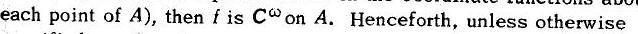
\includegraphics[max width=\textwidth]{image1.jpg}
specified, we let $r$ be $\infty, \omega$, or an integer $>0$.

A map $f$ from an open set $A \subset R^{n}$ into $R^{k}(k$ an integer $>1)$ is $C^{r}$ on $A$ if each of its slot functions $f_{i} \leq u_{i} \circ f$ is $C^{r}$ on $A$ for $i=1, \ldots, k$; thus for $p$ in $R^{n}, f(p)=\left(f_{1}(p), \ldots, f_{k}(p)\right)$ in $R^{k}$.

\includegraphics[max width=\textwidth]{2022_07_16_f4e476ee2159dc67e746g-04(4)}

Fig. 1.1 Overlapping Coordinate Domains

\section{Notes on Differential Geometry}
We now define a manifold. Let $M$ be a set. An n-coordinate pair on $M$ is a pair $(\phi, U)$ consisting of a subset $U$ of $M$ and 1 to 1 map $\phi$ of $U$ onto an open set in $R^{n}$. One $n$-coordinate pair $(\phi, U)$ is $C^{r}$ related to another $n$-coordinate pair $(\theta, V)$ if the maps $\phi \circ \theta^{-1}$ and $\theta^{\circ} \phi^{-1}$ are $C^{r}$ maps wherever they are defined (thus their domains of definition must be open). A $C^{r} n-S u b a t l a s$ on $M$ is a collection of $n$-coordinate pairs $\left(\phi_{h}, U_{h}\right)$, each of which is $C^{r}$ related to every other membor of the collection, and the union of the sets $U_{h}$ is $M .$ A maximal collection of $C^{r}$ related $n$-coordinate pairs is called a $C^{r} n$-atlas. If a $C^{r} n$-atlas contains a $C^{r} n-s u b a t l a s$, we say the subatl as induces or generates the atlas. Finally, an $n$ dimensional $C^{r}$ manifold or a $C^{r} n-m a n i f o l d$ is a set $M$ together with a $C^{r} n$-atlas. When $r=0, M$ is customarily called a locally Euclidean space or a topological manifold, and only when $r \neq 0$ is $M$ called a differentiable or smooth manifold. An atlas on a set $M$ is often called a differentiable structure or a manifold structure on $M$. Notice that one set may possess more than one differentiable structure (see example 4 below), however, a definition of "equivalent" differentiable structures is necessary before the study of different atlases on a set becomes meaningful (see Munkres ${ }^{1}$ ).

Each $n$-coordinate pair $(\phi, U)$ on a set $M$ induces a set of $n$ real valued functions on $U$ defined by $x_{i}=u_{i} \circ \phi$ for $i=1, \ldots, n$. The func tions $x_{1}, \ldots x_{n}$ are called coordinate functions or a coordinate system and $U$ is called the domain of the coordinate system.

We list some examples:

\begin{enumerate}
  \item Let $M$ be $R^{n}$ with a $C^{r} n-s u b a t l a s$ equal to the pair consisting of $\phi=$ the identity map and $U=R^{n}$.

  \item Let $M$ be any open set of $R^{n}$ and let a $C^{r} n-$ subatlas be (the identity $\operatorname{map}, M)$

  \item Let $M=G L(n, R)$, the group of non-singular $R-1$ inear transformations of $R^{n}$ into itself. Then $M$ can be mapped 1:1 onto an open set in $R^{n^{2}}$ and thus a manifold structure can be defined on $M$ via example 2. If $\left(a_{i j}\right)$ is a matrix representation of an element of $M$ with respect to the usual base of $R^{n}$, then map $\left(a_{i j}\right)$ into the $n^{2}$-tuple

\end{enumerate}
$\left(a_{11}, a_{12}, \ldots, a_{1 n}, a_{21}, a_{22}, \ldots, a_{2 n}, a_{31}, \ldots, a_{n n}\right)$

$\sqrt{ }$ The image set of this map will be open since it is the inverse image of an open set by the determinant map, which is continuous (indeed it is $C^{\omega}$ as a map on $R^{n^{2}}$ ).

\section{Chav. 1 Manifolds}
\begin{enumerate}
  \setcounter{enumi}{4}
  \item Let $M_{1}$ be the 1-dimensional $C^{1}$ manifold of example 1 , and let $M_{2}=R$ with the $C^{1}$ 1-subatlas $\left(\mathrm{x}^{3}, R\right)$, where $\mathrm{x}$ is the identity mapping on $R$. Then $M_{1} \neq M_{2}$ since $x^{1 / 3}$ is not $C^{1}$ at the origin.
\end{enumerate}
$\sqrt{ }$ 5. Let $f$ be a $C^{r}$ real valued function on $R^{n+1}$, with $r>0$ and $n>0$, and suppose the gradient of $f$ does not van ish on an $f$-constant set $M=\left[p\right.$ in $\left.R^{n+1}: f(p)=0\right]$. Then at each point in $M$, choose any partial derivative of $f$ that doesn't vanish, say the $i^{\text {th }}$ one, apply the implicit function theorem to obtain a neighborhood of $p$ (relative topology on $M$ ) which projects in a $1: 1$ way into the $u_{i}=0$ hyperplane of $R^{n+1}$, and thus define a subatlas which makes $M$ a $C^{r} n$-manifold.

This example covers many classical hypersurfaces in $R^{n+1}$, including spheres, planes, and cylinders.

$\sqrt{6}$. The process in example 5 can easily be generalized to obtain $C^{r}(n-k)$-manifolds from "constant sets" of a $C^{r} \operatorname{map} f: R^{n} \rightarrow R^{k}$ whose Jacobian matrix is of rank $k$ on the constant set.

\begin{enumerate}
  \setcounter{enumi}{7}
  \item Let $F$ be a univalent map from an open set in $R^{n}$ into $R^{m}$, with $0<n<m$, and let $M$ be the image of $F$. Then the $n$-coordinate pair $\left(F^{-1}, M\right)$ defines a $C^{r} n-$ subatlas on $M$.
\end{enumerate}
For further definitions, let $M$ be a fixed $C^{r} n$-manifold. An open set in $M$ is a subset $A$ of $M$ such that $\phi(A \cap U)$ is open in $R^{n}$ for every $n$-coordinate pair $(\phi, U)$. The reader can verify that $M$ becomes a topological space with this definition of the open sets. If $p$ in $M$, then a neighborhood of $p$ is any open set containing p. Notice $M$ need not be Hausdorff. The concept of Hausdorffness is irrelevant for much of local differential geometry. It becomes relevant in passing from a Riemannian metric to a distance function.

\section{Section 1.2 Smooth Functions}
In this section let $A$ be the domain of a function $f$ and assume $A$ is an open subset of the $C^{t} n$-manifold $M$. If $f$ is real valued, then $f$ is $C^{s}$ on $A$ isfo $\phi^{-1}$ is $C^{s}$ on $\phi(A \cap U)$ for every coordinate pair $(\phi, U)$ on $M .$ Note the independence of $r$ and s. If $N$ is a $C^{k} d-m a n i=$ fold and $f$ is $N$-valued, and $f$ is $C^{s}$ on $A$ if $f$ is continuous and for every real valued function $g$, that is $C^{s}$ on an open domain in $N$, the composite $g \circ f$ is $C^{s}$ on $A \cap f^{-1}$ (domain of $g$ ). Note the independence of $r, k_{\text {a d }}$ and.\\

\includegraphics[max width=\textwidth]{2022_07_16_f4e476ee2159dc67e746g-06}

Fig. 1.2 An Induced Map from $R^{2}$ into $R$

The local character of the smoothness of a function is captured in the following definition. Suppose the domain of $f$ is not necessarily open and $f$ is $N$-valued. If $p$ is in the domain of $f$, then $f$ is $C^{s}$ at $p$ if there is a neighborhood $U$ of $p$ with $f$ defined on $U$ such that $\left.f\right|_{U}$ is $C^{s}$ on $U$. As a corollary, if $f$ is $C^{s}$ at every point in its domain then its domain is open.

Let us now specialize to $C^{\infty}$ manifolds and $C^{\infty}$ functions. This is done for convenience chiefly and it allows us to define a tangent vector in a very elegant way. Our concern in these notes is not with "the least possible assumptions" but rather with those concepts that arise naturally in a general situation. The restriction is not too drastic because of the following result due to Whitney: A $C^{r}$ atlas on a set with $r>0$ contains a $C^{\infty}$ atlas (see Munkres ${ }^{1}$ ). There is an example of Kervaire which exhibits a $C^{0}$ atlas on a set which admits no $C^{1}$ atlas. For further work on the "equivalence" of differentiable structures see Milnor 1 and 2 , Munkres 1 and 2 , and Smale ${ }^{1}$.

The following list of nine problems are recommended in order to familiarize oneself with the notion of a $C^{\infty}$ map. In particular the problems are aimed at obtaining numbers 6 and 7 which are often useful. The list (remember $A$ is open in $M$, which is a $C^{\infty} n$-manifold);

\begin{enumerate}
  \item The map $f: A \rightarrow N$ is $C^{\infty}$ on $A$ iff $f$ is $C^{\infty}$ at each point $p$ in $A$.

  \item If $f: A \rightarrow N, f$ is $C^{\infty}$ on $A$, and $U$ is an open set contained in $A$, then $\left.f\right|_{U}$ is $C^{\infty}$ on $U$ 3. Let $U_{h}$ be a collection of open sets in $M$ and let $f_{h}: U_{h} \rightarrow N$ be $C^{\infty}$ on $U_{h}$ for each $h$. If $f$ is a function whose domain is the union of all $U_{h}$ and if $\left.f\right|_{U}=f_{h}$ for all $h$, then $f$ is $C^{\infty}$ on its domain.

  \item If $f: A \rightarrow R^{k}$ is $C^{\infty}$ on $A \subset R^{n}$ and $g: B \rightarrow R$ is $C^{\infty}$ on the open set $B \subset R^{k}$, then $g \circ f$ is $C^{\infty}$ on $A \cap f^{-1}(B)$.

  \item If $f: A \rightarrow N$ is $C^{\infty}$ on $A \subset M$ and $(\phi, U)$ is a coordinate pair on $M$, then $f \circ \phi^{-1}$ is $C^{\infty}$ on $\phi(A \cap U)$.

  \item Let $P$ be a $C^{\infty} s$-manifold. If $F: A \rightarrow N$ is $C^{\infty}$ on $A \subset M$ and $g: B \rightarrow P$ is $C^{\infty}$ on the open set $B \subset N$, then $g \circ f$ is $C^{\infty}$ on $A \cap f^{-1}(B)$.

  \item The map $f: A \rightarrow N$ is $C^{\infty}$ on $A \subset M$ iff for every coordinate pair $(\phi, U)$ in a subatlas on $N$ the functions $x_{i} \circ f$ are $C^{\infty}$ on $A \cap f^{-1}(U)$, for $i=1_{0}, \ldots, d$ and $x_{i}=u_{i} \circ \phi$.

  \item If $n \geq k$ and $g: R^{n} \rightarrow R^{k}$ by $g\left(a_{1}, \ldots, a_{n}\right)=\left(a_{1}, \ldots, a_{k}\right)$ then $g$ is $C^{\infty}$ on $R^{n}$. If $h: R^{k} \rightarrow R^{n}$ by $h\left(a_{1}, \ldots, a_{k}\right)=\left(a_{1}, \ldots, a_{k}, 0, \ldots, 0\right)$ then $h$ is $C^{\infty}$ on $R^{k}$.

  \item Let $f$ and $g$ be real valued functions that are $C^{\infty}$ on the subsets $A$ and $B$ of $M$, respectively. Show that $f+g$ and $f g$ are $C^{\infty}$ on $A \cap B$, where $(f+g)(p)=f(p)+g(p)$ and $(f g)(p)=f(p) g(p)$.

\end{enumerate}
For the record, we can and so do define a Lie group. A Lie group $G$ is a group $G$ whose underlying set is also a $C^{\infty}$ manifold such that the group operations are $C^{\infty}$, i.e. the map $\phi: G x G \rightarrow G$ where $\phi(g, h)=$ $g h^{-1}$ is $C^{\infty}$ (see problem 18 and 20$)$.

One last bit of notation, let $C^{\infty}(A, N)$ denote the set of $C^{\infty}$ functions mapping an open set $A$ in a manifold $M$ into a manifold $N$.



\section{Section $1.4$ The Jacobian of a map}
Let $M$ and $N$ be $C^{\infty}$ manifolds of dimensions $n$ and $k$ respectively. We defined above the concept of a $C^{\infty} \operatorname{map} f$ from $M$ into $N$. Such a map induces a linear transformation from each tangent space $M_{m}$ into the tangent space $N_{f(m)^{\circ}}$ This linear map is called the Jacobian map or the differential of $f$ and we denote it by $f_{*}$ (often it is de noted $d f$, but we reserve the symbol $d$ for the exterior derivative operator). Let $X$ be in $M_{m}$ and we define $f_{*} X$ as a vector at $f(m)$ in $N$ by taking a function $g$ which is $C^{\infty}$ in a neighborhood of $f(m)$ and setting $\left(f_{*} X\right) g=$ $X(g \circ f)$. It is trivial to check that $f * X$ is a vector at $f(m)$ and the map $f_{*}$ is linear.

By selecting a coordinate system $x_{1}, \ldots, x_{n}$ about $m$ and another $y_{1}, \ldots, y_{k}$ about $f(m)$, we can determine a matrix representation for $f_{*}$ which is called the Jacobian matrix of $f_{*}$ with respect to the chosen coordinate systems. Let $X_{i}=\partial / \partial x_{i}, Y_{j}=\partial / \partial y_{j}$, thus $X_{1}, \ldots, X_{n}$, at $m$, form a base for $M_{m}$ and we compute $f_{*}$ by computing its action on this base. Namely, $f_{*} X_{i}=\Sigma_{j}\left(f_{*} X_{i}\right) y_{j} Y_{j}$ by the representation theorem above, hence the matrix in question is the matrix $\left(\left(f_{*} X_{i}\right) y_{j}\right)=$ $\left(\partial\left(y_{j} \circ f\right) / \partial x_{i}\right)$ for $1 \leq i \leq n$ and $1 \leq j \leq k$

The implicit function theorem and the inverse function theorem can be applied and formulated in this language. The former we postpone, since we do not really need it for some time (see problem 16) but the latter is both useful and instructive. First a definition. A diffeomorphism is a map $f: M \rightarrow N$ that is $1: 1$ and onto with both $f$ and $f^{-1} C^{\infty}$,
$$
X(c)=c X(1)=c(1 X(1)+1 X(1))=2 c X(1)
$$
$$
\begin{aligned}
&=\Sigma_{i}\left[\left(X_{Y_{i}}\right) f_{i}(m)+y_{i}(m)\left(X f_{i}\right)\right. \\
&=\Sigma_{i} X\left(x_{i}-x_{i}(m)\right) f_{i}(m) \\
&=\Sigma_{i}\left(X_{X_{i}}\right)\left(\partial f / \partial x_{i}\right)(m)
\end{aligned}
$$
and if such an $f$ exists, then $M$ is diffeomorphic to $N$.

THEOREM. (Inverse function) Let $M$ and $N$ be $C^{\infty} n$-manifolds and let $f: M \rightarrow N$ be $C^{\infty}$. If for $m$ in $M$, the Jacobian $f_{*}$ at $m$ is an isomorphism of $M_{m}$ onto $N_{f(m)}$ then there is a neighborhood $U$ of $m$ and a neighborhood $V$ of $f(m)$ such that $f$ is a diffeomorphism from $U$ to $V$ (i.e., $f$ is a local diffeomorphism about $m$ ).

We leave it to the reader to choose a coordinate system on both sides and apply the theorem from advanced calculus to obtain the result. Notice the $C^{\infty}$ demand of $f$ and $f^{-1}$ implies the theorem could be stated as a necessary as well as a sufficient condition for the existence of a local inverse. If one only demands continuity of the inverse then the map $x \rightarrow x^{3}$ provides a homeomorphism of $R$ onto $R$ whose Jacobian is singular at the origin.

Now consider the behavior of the Jacobian with respect to composite maps. Let $g$ be a $C^{\infty}$ map of $N$ into the $C^{\infty}$ manifold $L$. Then at each $m$ in $M,(\xi \circ f)_{*}=g_{*} \circ f_{*}$, for if $h$ is a $C^{\infty}$ function about $g(f(m))$ and $X$ in $M_{m}$ then $\left((g \circ f)_{*} X\right) h=X(h \circ g \circ f)=\left(f_{*} X\right)(h \circ g)=$

\includegraphics[max width=\textwidth]{2022_07_16_f4e476ee2159dc67e746g-09}\\
hibits the chain rule and a multiplicative behavior of Jacobian matrices When $f$ is a diffeomorphism of $M$ into $N$, and $X$ and $Y$ are $C^{\infty}$ fields on $M$, then $f_{*} X$ and $f_{*} Y$ are $C^{\infty}$ fields on $N$ with $f_{*}[X, Y]=\left[f_{*} X, f_{*} Y\right]$



\section{Section $1.6$ Submanifolds}
A $C^{\infty} k$-manifold $M$ is a submanifold of a $C^{\infty} n$-manifold $\bar{M}$ if for every point $p$ in $M$ there is a coordinate neighborhood $\bar{U}$ of $\bar{M}$ with coordinate functions $\bar{x}_{1}, \ldots, \bar{x}_{n}$ such that the set $U=\left[m\right.$ in $\bar{U}: \bar{x}_{k+1}(m)=$ $\left.\ldots=x_{n}(m)=0\right]$ is a coordinate neighborhood of $p$ in $M$ with coordinate functions $x_{1}=\left.\bar{x}_{1}\right|_{U}, \ldots, x_{k}=\left.\bar{x}_{k}\right|_{U}$. These coordinate systems are called special or adapted coordinate systems.

Notice it is not required that $M \cap \bar{U}=U$ so "slices" of $M$ may approach other "slices ${ }^{n}$ of $M$ in $\bar{M}$ (see problem 17), and hence the topology on $M$ may not be the relative topology. The definition of submanifold implies $M$ is a subset of $\bar{M}$ and $k \leq n$. Letting $i: M \rightarrow \bar{M}$ be the inclusion map, then $i$ is $C^{\infty}$ since $\bar{x}_{j}, i$ are $C^{\infty}$ maps for all special coordinate functions. The inclusion map is also an imbedding (see below) since the Jacobian $i *$ is non-singular, i.e., $i_{*}\left(\partial / \partial x_{j}(p)=\right.$ $\partial / \partial \bar{x}_{j}(p)$ for $j=1, \ldots, k$. In these notes we will identify a tangent vec. tor $X$ in $M_{p}$ with its image in $\bar{M}_{p}$ unless there is a possibility of confusion (just as we identify $p$ and $i(p)$ ).

To make some more standard definitions, let $M$ and $\bar{M}$ be $C^{\infty}$ manifolds and let $f$ be a $C^{\infty}$ map of $M$ into $\bar{M}$. If $f_{*}$ is non-singular (thus $f_{*}$ has no kernel) at each point $p$ of $M$, then $f$ is called an immersion of $M$ into $M$. If in addition, $f$ is univalent, then $f$ is called an imbedding of $M$ into $\bar{M}$. A subset $M^{\prime}$ of $\bar{M}$ is called an immersed submanifold if there exists a manifold $M$ and an immersion $f: M \rightarrow \bar{M}$ such that $\dot{f}(M)=M^{\prime}$. (Thus an immersion is a "local imbedding with self-intersections.") One can verify (problem 17) that if $f: M \rightarrow \bar{M}$ is an imbedding and $M^{\prime}=f(M)$, then by defining a differentiable structure on $M^{\prime}$ so $f$ becomes a diffeomorphism, $M^{\prime}$ becomes a submanifold of $\bar{M}$ (see Helgason, p. 23).

For examples of submanifolds see the examples 5,6 , and 7 at the end of section $1.1$

It is convenient to define a base field on a set $A$ contained in an $n$-manifold to be a set of $n$ vector fields that are independent at each

\section{4}
Notes on Differential Geometry

point of $A$. When each field in a base field is $C^{\infty}$, then the base field is $C^{\infty}$. Since a set of coordinate fields is a $C^{\infty}$ base field on the coordinate domain, we know $C^{\infty}$ base fields always exist locally. A $C^{\infty}$ base field does not necessarily exist over a whole manifold (consider the 2«sphere, $S^{2}$ ); indeed, the manifold is called parallelizable if it admits a global $C^{\infty}$ base field.

We now define a concept which we will often use. Let $M$ be a submanifold of $\bar{M}$ as described above. An $\bar{M}$-vector field $Z$ that is $C^{\infty}$ on $M\left(\right.$ or $C^{\infty}$ on an open set $A$ in $M$ ) is a map that assigns to each $p$ in $M$

\includegraphics[max width=\textwidth]{2022_07_16_f4e476ee2159dc67e746g-11}\\
field on a neighborhood $\bar{U}$ of $p$ and $Z_{m}=\sum_{i}^{n_{i}} a_{i}(m)\left(X_{i}\right)_{m}$ for $m$ in $M \cap \bar{U}$ then the real valued functions $a_{i}$ are $C^{\infty}$ on $M \cap U$ for all $i$. Notice $Z$ is not necessarily tangent to $M$. Since the restriction to $M$, of a $C^{\infty} p$ function on $\bar{M}$, is a $C^{\infty}$ function on $M$, it follows if $Z$ is $C^{\infty}$ on $\bar{M}$ then $\left.Z\right|_{M}$ is an $\bar{M}$-vector field that is $C^{\infty}$ on $M$.

Problems (For problems 1 thru 9 see pages 4 and 5)

\begin{enumerate}
  \setcounter{enumi}{10}
  \item Let $W_{1}, \ldots, W_{n}$ be a $C^{\infty}$ base field on an open set $U$ in a manifold $M$ and let $X=\sum_{i=1}^{n} f_{i} W_{i}$ be a vector field on $U$. Show $X$ is $C^{\infty}$ on $U$ iff the functions $f$ are $C^{\infty}$ on $U$ for all $i$. If $Y$ and $Z$ are $C^{\infty}$ fields on $U$ show $[Y, Z]$ is $C^{\infty}$. Showi that a coordinate field $\partial / \partial x_{i}$ is $C^{\infty}$ on its domain. If $X$ is a given vector at $p$ in $M$ show there is a $C^{\infty}$ field $\bar{X}$ on a neighborhood of $p$ with $\bar{X}=X_{p}$. If $x_{1} \ldots, x$ is a coordinate system with domain $U$ and $A=\sum a_{i}\left(\partial / \partial \mathrm{x}_{i}\right)$ and $B=\sum b_{i}\left(\partial / \partial \mathrm{x}_{i}\right)$ are $C^{\infty}$ fields on $U$ then find the representation of $[A, B]$ in terms of the coordinate vector fields. Show $[f X, g Y]=f(X g) Y-g(Y f) X+f g[X, Y]$ where $X$ and $Y$ are $C^{\infty}$ fields on $U$ and $f$ and $g$ are in $C^{\infty}(U, R)$ Prove the Jacoby identity.

  \item Let $A, B$ and $C$ be in $C^{\infty}\left(R^{3}, R\right)$ with $B \neq 0$ anywhere. Let $V=A i+B j+C k, X=-B i+A j$, and $Y=-C j+B k$ (advanced calculus notation). For $p$ in $R^{3}$, let $P p=\left[Z\right.$ in $\left(R^{3}\right)_{p}$ : $\left.Z \cdot V_{p}=0\right]$. Show $P_{p}$ is a two-dimensional space of vectors at each point by showing $X_{p}$ and $Y_{p}$ are a base for $P_{p}$. Show $[X, Y]_{p}$ lies in $P_{p}$ iff $V_{p}{ }^{p}\left(\operatorname{curl} V_{p}=0\right.$. If there is a function $f$ in $C^{\infty}\left(R^{3}, R\right)$ with grad $f \neq 0$ such that $P$ is the tangent plane Chap. 1 Manifolds

\end{enumerate}
to the constant surface of $f$ thru $p$ show $V_{p^{\circ}}(\operatorname{cur} 1 V)_{p}=0$ (see section 9.1).

Instead of seeking surfaces that are orthogonal to $V$ (as above), one could seek surfaces whose tangent plane contains $V$ and then one has a "geometric quasi-linear partial differential equation of the first order." Integral curves of $V$ are called characteristics of the "equation." One generates solution surfaces by taking a non-characteristic curve (an "initial value ${ }^{n}$ curve) and considering the surface formed by characteristics thru the initial value curve. Show two solution surfaces must intersect along a characteristic. Show there are an infinite number of solution surfaces thru one characteristic. Can there there be an initial value curve with no solution thru it?

\begin{enumerate}
  \setcounter{enumi}{12}
  \item Let $f: R^{2} \rightarrow R^{2}$ by $f(a, b)=\left(a^{2}-2 b, 4 a^{3} b^{2}\right)$ and let $g: R^{2} \rightarrow$ $R^{3}$ by $g(u, v)=\left(u^{2} v+v^{2}, u-2 v^{3}, v e^{u}\right)$. Compute a matrix for $f *$ at $(1,2)$ and $g *$ at any $(u, v)$. Find $g_{*}(4 \partial / \partial x-\partial / \partial y)(0,1)^{*}$ Find integral curves for the vector field $X=y i+y j+2 k$ on $R^{3}$. Find a coordinate system $x_{1}, x_{2}, x_{3}$ on $R^{3}$ such that $\partial / \partial x_{1}=2 i+3 j-k$ at all points.

  \item Let $X$ and $Y$ be $C^{\infty}$ fields about $m$ in $M$. For small $t \geq 0$ define the curve $\sigma(t)$ as follows: go $t$ parameter units on $X$ integral curve thru $m$ to $p_{1}$, go $t$ units on $Y$ curve thru $p_{1}$ to $p_{2}$, go $t$ units on $(-X)$ curve thru $p_{2}$ to $p_{3}$ go $t$ units on $(-Y)$ curve thru $p_{3}$ to $\sigma(t)$. If $\gamma(t)=\sigma(\sqrt{ } t)$ show $T_{\gamma}(0)=[X, Y]_{m}$. (Hint: use the lemma in section $9.1$ and partial Taylor series.)

  \item Let $M$ and $N$ be manifolds with $M$ connected and let $f$ and $g$ be $C^{\infty}$ maps of $M$ into $N$. Show $f_{*} \equiv 0$ iff $f$ is a constant map. If $f(m)=g(m)$ at one $m$ in $M$ and $f_{*} \equiv g_{*}$ at all points show $f=\delta$.

  \item Let $f$ be in $C^{\infty}(M, R)$ and define the differential of $f$, df to be the linear map of $M$ into $R$ where $(d f)(X)=X$, . Show $f_{*}\left(X_{m}\right)=[(d f)(X)](\partial / \partial t)$ where $t$ is the identity coordinate $f_{*}\left(X_{m}\right)=\left[(d f)_{m}(X)\right](\partial / \partial t)$ where $t$ is the identity coordinate\\
function on $R$. It is because of this case that in a general function on $R .$ It is because of this case that in a general

  \item Prove the Inverse Function Theorem (p.10) of state and prove a version of the Implicit Function Theorem of advanced calculus in terms of the Jacobian map. 17. Prove the last sentence in the third paragraph of section 1.6. Show that the image of a regular $\left(\sigma_{*} \neq 0\right)$ univalent curve $\sigma$ mapping an open interval into a manifold $M$ is a one-dimensional submanifold of $M$. Let $X$ be a unit constant vector field on $R^{2}$ with irrational slope. Let $T$ be the set of equivalence classes on $R^{2}$ where $(a, b) \sim(c . d)$ iff $a-c=n$ and $(b-d)=m$ for integers $m$ and $n .$ Show $T$ is a two-dimensional manifold (which is called the flat torus) in a natural way. Show $X$ in duces a vector field on $T$ such that the image of one integral curve of $X$ defines a one-dimensional submanifold of $T$ that is dense in $T .$

  \item Let $M_{1}$ and $M_{2}$ be $C^{\infty}$ manifolds. Let $\pi_{i}: M_{1} \times M_{2} \rightarrow M_{i}$ by $\pi_{i}\left(m_{1}, m_{2}\right)=m_{i}$ for $i=1$,2. Define a $C^{\infty}$ structure on $M_{1} \times$ $M_{2}$ so $\pi_{i}$ are $C^{\infty} .$ Show $\left(M_{1} \times M_{2}\right)_{\left(m_{1}, m_{2}\right)}$ is naturally isomorphic to $\left(M_{1}\right)_{m,} \times\left(M_{2}\right)_{m_{2}}$.

  \item Let $M$ be a $C^{\infty} n-$ manifold. Let $T(M)=\left[(m, X): X\right.$ in $\left.M_{m}\right]$, and let $\pi: T(M) \rightarrow M$ by $\pi(m, X)=m .$ If $(\phi, U)$ is a coordinate

\end{enumerate}
\includegraphics[max width=\textwidth]{2022_07_16_f4e476ee2159dc67e746g-12}\\
$(m, X)$ in $\bar{U}$ let $x_{i}(m, X)=a_{i}$ if $X=\sum a_{i}\left(\partial / \partial x_{i}\right)$. Let $\bar{\phi}: \bar{U} \rightarrow$ subatlas of pairs ${ }^{2 n} u_{i} \circ \phi=\bar{x}_{i}$ and $u_{n+i} \circ \phi=\dot{X}_{i}$ for $i=1, \ldots, n$. Show the subatlas of pairs $(\bar{\phi}, \bar{U})$ defines a $C^{\infty}$ structure on $T(M)$ which is called the tangent bundle of $M$. If $f$ is a $C^{\infty}$ map of $M$ into $N$ show $f_{*}$ induces a $C^{\infty}$ map of $T(M)$ into $T(N)$

\begin{enumerate}
  \setcounter{enumi}{20}
  \item Let $G$ be a Lie group. If $g$ in $G$ let $L_{g}, R_{g^{\prime}}$ and $A_{g}$ denote the maps of $G$ into $G$ defined by $L_{g}(h)=g h, R_{g}^{g}(h)=h g$, and $A_{g}(h)=g h g^{-1} \cdot$ Show $L_{\theta}, R_{\theta^{\prime}}$, and $A_{G}$ are $C^{\infty}$, A vector field $X$ on $G$ is left invariant if $\left(L_{\beta}\right)_{*} X_{\theta}=X_{\beta h}$ for all $g$ and $h$. Show a left invariant field is $C^{\infty}$ and is completely determined by its value at the identity e. If $X$ and $Y$ are left invariant showy $[X, Y]$ is left invariant. The set of left invariant vector fields on $G$ forms an $n$ dimensional vector space called the $L$ ie algebra of $G$ which is denoted by g. Define a one-parameter sub group of $G$ to be the image of a $C^{\infty}$ homormorphism of $R$ into G. Show there is a 1:1 correspondence between one-parameter subgroups and integral curves of left invariant vector fields thru e. Show the map $(\xi, h) \rightarrow \rightarrow^{-1}$ is $C^{\infty} f$ tom $G \times G$ into $G$ iff the maps $(g, h) \rightarrow g h$ and $g \rightarrow g^{-1}$ are $C^{\infty}$.

  \item Let $G=G L(n, R)$ and for a matrix $g$ in $G$ let $u_{i j}(g)=g_{i j}$ (see example 3). Call $u_{i j}$ the natural coordinate functions on $G_{.}$ Write $u_{i j} \cdot L_{g}$ as a linear combination of the ratural coordinate functions. Let $X_{i j}$ be the unique left invariant field on $G$ with $X_{i j}(e)=\left(\partial / \partial u_{i j}\right)(e)$ where e is the identity element. Compute $X_{i j}$ as a field on $G$ in terms of the coordinate vector fields. Compute $\left[X_{i j}, X_{r s}\right]$. If $A(t)$ is a $C^{\infty}$ curve in $G$ with $A(0)=e$ and $A(t)$ orthogonal for all $t$ show $d A / d t=\left(d a_{i j} / d t\right)$ is a skewsymmetric matrix for $t=0$.

  \item Let $M$ be a $C^{\infty} n-m a n i f o l d .$ Let $B(M)=\left[\left(m ; e_{1}, \ldots, e_{n}\right): m\right.$ in $M$ and $e_{1}, \ldots, e_{n}$ an ordered based of $\left.M_{m}\right]$. Let $\pi: B(M) \rightarrow M$ by $\pi\left(m ; e_{1}, \ldots, e_{n}\right)=m .$ If $(\phi, U)$ a coordinate pair on $M$ with $x_{i}$ $=u_{i} \cdot \phi$, let $(\bar{\phi}, \bar{U})$ be a coordinate pair on $B(M)$ with $\bar{U}=\pi^{-1}(U)$ and $\bar{\phi}: \bar{U} \rightarrow R^{n+n^{2}}$ by the coordinate functions $\bar{x}_{1}, \ldots, \bar{x}_{n}$, $x_{11}, x_{12}, \ldots, x_{n n}$ where $\bar{x}_{i}=x_{i} \cdot \pi$ and if $b=\left(m ; e_{1, \ldots,}, e_{n}^{n}\right)$ then $e_{j}=\sum_{i=1}^{n} x_{i j}(b)\left(\partial / \partial x_{i}\right)$. Show the subatlas of pairs $(\bar{\phi}, \bar{U})$ defines a $C^{\infty}$ structure on $B(M)$ which is called the bundle of bases over M. For $g$ in $G L(n, R)$ let $R_{B}: B(M) \rightarrow B(M)$ by $R_{g}(b) \equiv b g \equiv\left(m ; \sum_{i=1}^{n} g_{i 1} e_{i}, \sum_{i} g_{12} e_{i}, \ldots, \Sigma_{i} g_{i n} e_{i}\right)$ if $b=\left(m ; e_{1}, \ldots e_{n}\right)$. Show $R_{B}$ is $C^{\infty} \cdot$ Let $_{U}: U \rightarrow B(M)$ by $s_{U}(m)=\left(m ;\left(\partial / \partial x_{1}\right)\right.$ ,..., $\left.\left(\partial / \partial x_{n}\right)_{m}\right)$ for $m$ in $U$. Show $s_{U}$ is $C^{\infty}$ and $\pi \cdot s_{U}$ is the identity on $U$. The map $s_{U}$ is called the coordinate section map over $U_{0}$ Let $\hat{\phi}: U \times G L(n, R) \rightarrow \bar{U}$ by $\hat{\phi}(m, g)=R$ $s_{U}(m)=s_{U}(m) g .$ Show $\hat{\phi}$ is a diffeo onto its image. The map $\hat{\phi}$ is called a strip map. If $(\phi, U)$ and $(\psi, V)$ are coordinate pairs on $M$ define $s_{U V}: U \cap V \rightarrow G L(n, R)$ by $s_{U V}(m)=g$ if $s_{U}(m) g=s_{V}(m)$. Show $s_{U V}$ is $C^{\infty}$; it is called a structural function for $B(M)$. Show $\left(b g_{1}\right) g_{2}=b\left(g_{1} g_{2}\right)$ which justifies the name right action for $R \ldots$ For fixed $b$ in $B(M)$ let $f_{b}: G L(n, R) \rightarrow$ $B(M)$ by $f_{b}(g)=b g .$ Show $f_{b}$ is $C^{\infty} .$ Call the set $F b^{-1}(m)$ the (vertical) fiber over $m$ in $M$. Show $F$ is an $n^{2}-$ submanifold of $B(M)$ and $f_{b}$ is a diffo of $G L(n, R)$ onto $F, \pi(b)=$ $\pi(c)$, show $f^{-1} \circ f_{b}$ is a left translation on $G L(n, R)$. vector $X$ on $B(M)$ such that $\pi_{*}(X)=0$ is called a vertical vector. For $b$ in $B(M)$, let $E_{i j}(b)=\left(f_{b}\right), X_{i j}(e)$ define a vector $E(b)$ (cee problem 21). Show $E_{i j}$ is a global $C^{\infty}$ vertical vector field on $B(M)$. Compute $\left[E_{i j}, E_{r s}\right]$.

\end{enumerate}
\section{Hypersurfaces of $R^{n}$}


Section $2.1$ The standard connexion on $R^{n}$.



Section 2.2 The sphere map and the Weingarten map.

An $(n-1)$-submanifold of an $n$-manifold is called a hypersurface. Throughout this section let $M$ be a hypersurface of $R^{n}$, let $\bar{D}$ be the natural connexion on $R^{n}$, and assume $N$ is a unit normal vector field that is $C^{\infty}$ on $M$. Thus $\left\langle N_{p}, N_{p}\right\rangle=1$ and $\left\langle N_{p}, X\right\rangle=0$ for all $p$ in $M$ and $X$ in $M_{p} .$ Such an $N$ always exists locally.

For any $p$ in $M$ and any vector $X$ in $M_{p}$, define the linear map $L: M_{p} \rightarrow M_{p}$ by

(7) $L(X)=\bar{D}_{X} N$.

The vector $L(X)$ lies in $M_{p}$, since $0=X<N, N>=2<L(X), N>$ by property (6) for $\bar{D}$. The map $L$ is linear by properties (2) and (3). The map $L$ is called the Weingarten map, and in the case of $R^{n}$, it has a geometric interpretation as the Jacobian of the sphere map (Gauss map) which we now explain. Let $N=\left(a_{1}, \ldots, a_{n}\right)$, so the $a_{i}$ are real valued $C^{\infty}$ functions on $M$ and $\Sigma(a)^{2}=1$. Then the map $\eta: M \rightarrow S^{n-1}$ defined by $\eta(p)=\left(a_{1}(p)\right.$, $\left.\cdots, a_{n}(p)\right)$ in $R^{n}$, is a $C^{\infty}$ map of $M$ into the unit $(n-1)$-sphere $S^{n-1}$, and $\eta$ is called the sphere map (or Gauss map). If $X$ in $M_{p}$ and $\sigma(t)$ is a curve fitting $X$ (so $\sigma(0)=p$ and $\left.T_{\sigma}(0)=X\right)$, then $\eta \circ \sigma^{p}(t)=\left(a_{1} \circ\right.$ $\left.\sigma(t), \ldots, a_{n} \circ \sigma(t)\right)$ and
$$
\begin{aligned}
\eta_{*}(X) &=T_{\eta_{\sigma}}(0)=\left(\frac{d\left(a_{1} \circ \sigma\right)}{d t}(0), \ldots, \frac{d\left(a_{n} \circ \sigma\right)}{d t}(0)\right) \\
&=\left(X a_{1}, \ldots, X a_{n}\right)=\bar{D}_{X} N=L(X) .
\end{aligned}
$$
The map $L$ is $C^{\infty}$ on $M$ in the sense that if $X$ is $C^{\infty}$ on the subset $A$ of $M$ then $L(X)=\left(X a_{1}, \ldots, X a_{n}\right)$ is also $C^{\infty}$ on $A$ since each $a_{1}$ is C $^{\infty}$ on $M .$

\includegraphics[max width=\textwidth]{2022_07_16_f4e476ee2159dc67e746g-15}

Fig. 2.1 The Weingarten Map (derivative of normal)

Our next objective is to show $L$ is self-adjoint or symmetric; i.e., if $X, Y$ are in $M$ then $\langle L(X), Y\rangle=\langle X, L(Y)\rangle$.

To do this, let $Z$ be a $C^{\infty}$ field defined on a special coordinate neighborhood $U$ of $p$ and let $\bar{U}$ be the associated coordinate neighborhood of $p$ in $R^{n}$ with coordinate functions $\bar{x}_{1}, \ldots, \bar{x}_{n}$. Then $Z=\sum_{i=1}^{n-1}$ $g_{i}\left(\partial / \partial x_{i}\right)$, where $g_{i}$ are $C^{\infty}$ real valued functions on $U_{.}$We want to extend $Z$ to a $C^{\infty}$ field $\bar{Z}$ on $\bar{U}$, i.e., we want $\bar{Z}$ so that $\bar{Z}=Z$ for $p$ in $U$. Let us assume the coordinate map $\phi$ maps $\bar{U}$ onto a ba11 $B$ about the origin in $R^{n}$, i.e., $\bar{x}_{i}(p)=0=u_{\dot{i}} \cdot \vec{\phi}(p)$ for all i. Then if $\left(t_{1}, \ldots, t_{n}\right)$ is in $B$, let $\pi:\left(t_{1}, \ldots, t_{n}\right) \rightarrow\left(t_{1}, \ldots, t_{n-1}, 0\right)$. This map $\pi$ (which is $C^{\infty}$ ) induces a $C^{\infty} \operatorname{map} \sigma: \bar{U} \rightarrow U$ by $\sigma=\bar{\phi}^{-1} \cdot \pi \cdot \bar{\phi}_{0}$ Letting $\bar{Z}=\sum_{1}^{n-1}\left(g_{i} \circ \sigma\right)\left(\partial / \partial \bar{x}_{i}\right)$, the field $\bar{Z}$ is a $C^{\infty}$ extension of $\bar{Z}$ to $\bar{U}$

Actually the above process allows us to extend an $R^{n}$-field $Z$ that is $C^{\infty}$ on $U$ to a $C^{\infty}$ field $\bar{Z}$ on $\bar{U}_{.}$

Having the existence of such extensions we prove a proposition.

PROPOSITION. Let $U$ and $U$ be special neighborhoods of $p$ as above and let $Z$ and $Z$ be $C^{\infty}$ fields on $\bar{U}$ and $U$, respectively. Then $\bar{Z}$ is an extension of $Z$ (i.e., $\bar{Z} p_{p}=i_{*}\left(Z_{p}\right)$ for $p$ in $\left.U\right)$ iff $\left.(\bar{Z} f)\right|_{U}=Z\left(\left.f\right|_{U}\right)$ for all $f$ in $C^{\infty}(\bar{U}, R)$. If $\bar{X}$ and $\bar{Y}$ are $C^{\infty}$ extensions to $\vec{U}$ of $C^{\infty}$ fields $X$ and $Y$ on $U$, then $[\bar{X}, \bar{Y}]$ is a $C^{\infty}$ extension of $[X, Y] .$

Proof. If $\bar{Z}_{p}=i_{*}\left(Z_{p}\right)$ for $p$ in $U$, where $i: M \rightarrow R^{n}$ is the inclusion, then for $f$ in $C^{\infty}(\bar{U}, R),\left(\bar{Z}_{f}\right)(p)=\bar{Z}_{p} f=\left(\dot{t}_{*}\left(Z_{p}\right)\right) f=Z_{p}(f \circ \dot{i})=Z\left(\left.f\right|_{U}\right)(p)$. Conversely, if the two extreme terms are equal, then the second equality follows.

For the rest of the proposition, consider for $p$ in $U$
$$
\begin{aligned}
{[\bar{X}, \bar{Y}]_{p} f } &=\bar{X}_{p}(\bar{Y} f)-\bar{Y}_{p}(\bar{X} f)=X_{p}\left(\left.(\bar{Y} f)\right|_{U}\right)-Y_{p}\left(\left.(\bar{X} f)\right|_{U}\right) \\
&=X_{p}\left(Y\left(\left.f\right|_{U}\right)-Y_{p}\left(X\left(\left.f\right|_{U}\right)=[X, Y]_{p}\left(\left.f\right|_{U}\right)\right.\right.
\end{aligned}
$$
thus $[\bar{X}, \bar{Y}]$ is an extension of $[X, Y] . / /$

THEOREM. The Weingarten map is self-adjoint.

Proof. Take $X$ and $Y$ in $M_{p}$, imbed $X$ and $Y$ in $C^{\infty}$ fields on a special neighborhood $U$ of $p$, and extend $X$ and $Y$ to $C^{\infty}$ fields $\bar{X}$ and $\bar{Y}$ on $\bar{U}$ as above. Then

$\langle L X, Y\rangle-\langle X, L Y\rangle=\left\langle\bar{D}_{X} N, Y\right\rangle-\left\langle X, \bar{D}_{y} N\right\rangle$

$=\left\langle\bar{D}_{\vec{x}}-\bar{N}, \bar{Y}\right\rangle_{p}-\left\langle\bar{X}, \bar{D}_{-\bar{Y}} \bar{N}_{p}\right.$

$=\bar{X}_{p}\langle\bar{N}, \bar{Y}\rangle-\left\langle\bar{N}, \bar{D}_{\bar{x}} \bar{Y}_{p}-\bar{Y}_{p}\langle\bar{N}, \bar{X}\rangle+\left\langle\bar{N}, \bar{D}_{\bar{y}} \bar{X}_{p}\right.\right.$

$=\left\langle\bar{D}_{\bar{y}} \bar{X}-\bar{D}_{\bar{x}} \bar{Y}, \bar{N}\right\rangle_{p}$

$=\langle[\bar{Y}, \bar{X}], \bar{N}\rangle_{p}=\left\langle[Y, X]_{p}, N_{p}\right\rangle=0$,

\section{Notes on Differential Geometry}
since $\bar{X}_{p}\langle\bar{N}, \bar{Y}\rangle=X_{p}\langle N, Y\rangle=0=Y_{p}\langle N, X\rangle . / /$

The fundamental forms on $M$ can now be defined in terms of $L$ and the inner product. If $X$ and $Y$ are in $M_{p}$, then $I(X, Y)=\langle X, Y\rangle$, $I(X, Y)=\langle L(X), Y\rangle, I I I(X, Y)=\left\langle L^{2}(X), Y\right\rangle, I V(X, Y)=\left\langle L^{3}(X), Y\right\rangle$, mental torms on $M$ rors are called the first, second, third, etc. fundatensor defined ber $M$. Notice $M$ is a Riemannian manifold with metric is symmetric and the first fundamental form. Since the inner product is symmetric and $L$ is self-adjoint, the fundamental forms are all are $C^{\infty}$ in the sense that if $X$ and $Y_{p}$ for all $p$ in $M$. These forms are $C^{\infty}$ in the sense that if $X$ and $Y$ are $C^{\infty}$ fields with domain $A$, then $\left\langle L^{k}(X), Y\right\rangle_{p}=\left\langle L^{k}\left(X_{p}\right), Y_{p}\right\rangle$ is a $C^{\infty}$ real valued function on $A$. The first three forms have a direct interpretation geometrically since represents the Jacobian of the sphere map.

The algebraic invariants of the linear map $L$ at each point now depoint. Thus the geometric invariants of the submanifold $M$ at each point. Thus the determinant of $L$ at $p$ is the total curvature (Gauss $H(p)$, etc. $H(p)$, etc. The eigenvalues of $L$ are the principal curvatures and the igenvectors of $L$ are the directions of curvature or principal vectors. Since $L$ is self-adjoint there are always $(n-1)$ independent directions of curvature. If $L$ is a multiple of the identity map on $M$, then $p$ is an umbilic point of $M$. If $L=0$ at $p$ we call $p$ a flat point of $M$. Nonzero vectors $X$ and $Y$ in $M_{p}$ are conjugate if $\langle L X, Y\rangle=0$. A vector $X($ not zero) is asymptotic if it is self-conjugate, i.e., if $<L X, X>=0$ A curve in $M$ is a line of curvature if its tangent is a principal vector at each of its points.

The following facts come immediately from these definitions. An asymptotic direction $X$ is a direction of curvature iff $L X=0$ iff $X$ is $L \boldsymbol{X} \neq 0$ then there exists in Conjugate directions always exist since if $L X \neq 0$ then there exists a $Y$ which is orthogonal to $L X$. If the second fundamental form $<L X, Y>$ is positive or negative definite no asymptotic directions exist. If $X$ and $Y$ are two directions of curvature belonging to unequal eigenvalues, then $X$ is orthogonal to $Y$. The proof of this is standard algebra, i.e.,

$0=\langle L X, Y\rangle-\langle X, L Y\rangle=\left\langle k_{1} X, Y\right\rangle-\left\langle X, k_{2} Y\right\rangle=\left(k_{1}-k_{2}\right)\langle X, Y\rangle$,

\section{Chap. 2 Hypersurfaces of $R^{n}$}
so $k_{1} \neq k_{2}$ implies $\langle X, Y\rangle=0$. If $X$ and $Y$ are non-zero independent vectors with $L X=k X$ and $L Y=-k Y$, then the vectors $X+Y$ and $X$ - $Y$ are orthogonal asymptotic directions spanning the same subspace as $X$ and $Y$. Finally one notices that $L$ must satisfy its characteristic polynomial, which will also give a relation between the fundamental forms, i.e., if $n=3$, then $L^{2}-H L+K$ (identity) $=0$ and $I I I-H I I+K I=0$

When $X$ is a principal vector, the Weingarten map says $\bar{D}_{X} N=k X$, where $k$ is a principal curvature, and this equality is clas sically called the formula of Rodrigues.

Another classical concept is the Dupin indicatrix at each $p$ in $M$ which is the subset of $M_{p}$ consisting of all vectors $X$ such that $<L(X), X>=\pm 1$

Let $n=3$ and let $X$ and $Y$ be unit orthogonal principal vectors in $M_{p}$ with $L X=k X$ and $L Y=h Y$. If $Z=a X+b Y$, then $\langle L Z, Z\rangle=k a^{2}+$ $h b^{2}$. Thus the indicatrix is the curve (or curves) in $M$ such that $k a^{2}+h b^{2}=\pm 1$. Consider the three cases:

(1) If $K(p)>0$, then $h$ and $k$ have the same $\operatorname{sign}($ for $K=h k=$ det $L)$ so suppose they are positive. The indicatrix is then an ellipse determined by $k a^{2}+h b^{2}=1$, and $p$ is an elliptic point.

(2) If $K(p)<0$, then $h$ and $k$ have opposite signs, the indicatrix is two hyperbolas, and $p$ is a hyperbolic point.

(3) If $K(p)=0$, say $k=0, h>0$, then $b=\pm 1 / \sqrt{h}$ gives two straight lines parallel to the $X$ vector, and $p$ is a parbolic point. (When $k=h=0, p$ is an umbilic and a flat point.)

There is a geometric interpretation of the indicatrix as an approxi mation to the intersection of the surface with a plane which is parallel and close to the tangent plane; for details see Struik (p. 84).

Section $2.3$ The Gauss equation.

As in the last section, let $M$ be a hypersurface of $R^{n}$, let $\bar{D}$ be the natural connexion on $R^{n}$, let $N$ be a unit normal field that is $C^{\infty}$ on $M$, and let $L(X)=\bar{D}_{X} N$ for $X$ tangent to $M .$ Let $U$ and $\bar{U}$ be special coordinate neighborhoods of a point $p$ in $M$ and $R^{n}$ respectively, and let $\bar{Z}$ be a $C^{\infty}$ extension to $\bar{U}$ of a $C^{\infty}$ field $Z$ on $U$ as usual. If $Y$ is a $C^{\infty}$ field about $p$ in $M$, and $X$ in $M_{p}$, define $D_{X} Y$ by

\includegraphics[max width=\textwidth]{2022_07_16_f4e476ee2159dc67e746g-17}

Fig. 2.2 Decomposition of $\bar{D}_{X} \boldsymbol{Y}$

Since the Gauss equation induces a connexion $D$ on $M$, one can define parallel vector fields along a curve and geodesics exactly as in section 2.1. If $\sigma$ is a $C^{\infty}$ curve in $M$ with tangent $T$ and $Y$ is a $C^{\infty}$ field along $\sigma$, then $Y$ is parallel along $\sigma$ if $D_{T} Y=0$ along $\sigma$. The curve $\sigma$ is a geodesic if $D_{T} T=0$ along $\sigma$.

Application of the Gauss equation to the tangent field along a curve gives two results immediately.

THEOREM. Let $M$ be a hypersurface in $R^{n}$. A curve in $M$ is a geodesic in $R^{n}$ iff it is an asymptotic geodesic in $M$. $A$ curve in $M$, which is not a geodesic in $R^{n}$, is a geodesic in $M$ iff $\bar{D}$ is normal to $M$ along the curve (whose tangent is $T$ ).

Proof. Let $g$ be a curve in $M$ with tangent $T_{\text {. The Gauss equation }}$ The The implies $\bar{D}_{T} T=D_{T} T-<L T, T>N_{0}$. Thus $\bar{D}_{T} T=0$ iff $D_{T} T=0$ and $\langle L T, T\rangle=0$. And $D_{T} T=0$ iff $\bar{D}_{T} T$ is normal to $M \cdot / /$

Corollary. If $M_{1}$ and $M_{2}$ are two hypersurface s of $R^{n}$ and $\xi$ is a geodesic on both hypersurfaces that is not a geodesic in $R^{n}$, on any parameter interval, then $M_{1}$ and $M_{2}$ are tangent along $g\left(i_{0} e_{.}\right.$, their tangent spaces coincide along $g$ ).

Proof. Let $T$ be the tangent to $g_{0}$ Since $\bar{D}_{T} T \neq 0$ on any parameter interval, the normals to $M_{1}$ and $M_{2}$ determine the same subspace on a dense set of the parameter domain. Hence $M_{1}$ and $M_{2}$ are tangent along g./

(8) $D_{X} Y=\bar{D}_{X} Y-\langle L X, Y\rangle N$.

This is the Gauss equation. First notice $D_{X} Y$ is in $M_{p}$ for
$$
\left\langle D_{X} Y, N\right\rangle=\left\langle\bar{D}_{X} Y, N\right\rangle+\left\langle\bar{D}_{X} N, Y\right\rangle=X\langle Y, N\rangle=0 \text {. }
$$
since $\langle Y, N\rangle=0$ in a neighborhood of $p$. Next notice if $X, Y$ are $C^{\infty}$ on $U$, then $\bar{D}_{X} Y=\left.\bar{D}_{\bar{X}} \bar{Y}\right|_{U}$ and $\left\langle L X, Y>N\right.$ are both $C^{\infty}$ on $U$, so $D_{X} Y$ is $C^{\infty}$ on $U$; because of this, we say $D$ is $C^{\infty}$.

Thus $D$ becomes a candidate to define a covariant differentiation or a connexion on the submanifold $M$ which is defined very simply from the natural connexion on $R^{n}$ by decomposing $\bar{D}_{X} Y$ into its uniqus tangent and normal components relative to the tangent space of $M .$

One must now check if the properties $(1),(2),(3)$, and (4) are satisfi for $D$, and indeed they are, since they are satisfied for $\bar{D}$ and the sec. ond fundamental form is bilinear. The properties (5) and (6) are also. valid for $D$, so $D$ is the natural Riemannian connection associated with the induced metric (first fundamental form) on $M$ (see Chapter 6). The proof of the first four properties is left to the reader, but we now t: show (5) and (6). Let $Y$ and $Z$ be fields on a neighborhood $U$ about $p$, let $\bar{Y}$ and $\bar{Z}$ be extensions to $\bar{U}$, and let $X$ be in $M_{p}$. Then
$$
\begin{aligned}
\left(D_{Y} Z-D_{Z} Y\right)_{p} &=\left(\bar{D}_{Y} Z-\bar{D}_{Z} Y\right)_{p}=(\bar{D}-\bar{Y}-\bar{D} \bar{Z} \bar{Y})_{p} \\
&=[\bar{Y}, \bar{Z}]_{p}=[Y, Z]_{p}
\end{aligned}
$$
and
$$
\begin{aligned}
X\langle Y, Z\rangle &=X<\bar{Y}, \bar{Z}\rangle=\left\langle\bar{D}_{X} \bar{Y}, \bar{Z}\right\rangle+\left\langle\bar{Y}, \bar{D}_{X} \bar{Z}^{\prime}\right.\\
&=\left\langle D_{X} Y, Z_{p}\right\rangle+\left\langle Y_{p}, D_{X} Z\right\rangle .
\end{aligned}
$$
Thus the natural metric tensor and connexion on $R^{n}$ induce a Riemannian metric and Riemannian connexion on the hypersurface M.

\section{Notes on Differential Geometry}
Section 2.4. The Gauss curvature and Codazzi-Mainardi equations.

Let $M, N, L, D$ and $\bar{D}$ be as in the previous two sections. Our current goal is the "theorema egregium" of Gauss. This will show the "curvature" is independent of the imbedding, and motivate the definition of Riemannien curvature and curvature of a general connection.

Let $X, Y$, and $Z$ be $C^{\infty}$ fields on an open set $A$ in $M$. Notice that
$$
\begin{aligned}
&\bar{D}_{X}\left(\bar{D}_{Y} Z\right)-\bar{D}_{Y}\left(\bar{D}_{X} Z\right)-\bar{D}_{[X, Y]} Z \\
&\quad=\left(X Y Z_{1}, \ldots, X Y_{Z_{n}}\right)-\left(X Y_{Z_{1}}, \ldots, Y X z_{n}\right)-\left([X, Y] z_{1}, \ldots,[X, Y]_{n}\right)=0
\end{aligned}
$$
where $Z=\left(z_{1}, \ldots, z_{n}\right)$ and $z_{i}$ are $C^{\infty}$ real valued functions on $A$. This fact will later verify that the "curvature of $R^{n}$ is zero." By applying the Gauss equation and decomposing the above expression into tangent and normal parts, one obtains the Gauss curvature (9) and CodazziMainardi (10) equations, respectively.
$

\section{Section 2.5. Examples.}
See Figure $2.3$ for sketches of (1), (2), and (3).

\begin{enumerate}
  \item Let $M$ be an $(n-1)$ dimensional hyperplane in $R^{n}$, i.e., let $N=\left(a_{1,0,0}, a_{n}\right)$ determine a constant unit normal field on $M$. Then $L(X)=D_{X} N=\left(X a_{1}, \ldots, X a_{n}\right)=0$ for all $X$ at all points of $M$, i.e., $L \equiv 0$ on all of $M$. Thus $M$ consists entirely of flat (umbilic) points, the total curvature $K$ and mean curvature $H$ (and all others) are identically zero. All the fundamental forms except the first, are completely singular. Every victor is asymptotic and a direction of curvature, and all principal curvatures are zero.

  \item Let $M$ be $S$, the unit sphere about the origin in $R^{n}$, and let $N$ be the outer normal on $S_{,}$i.e., if $p=\left(a_{1}, \ldots, a_{n}\right)$ then $N(p)=\left(a_{1},\right.$, *..g $\left.a_{n}\right)$. Thus the sphere map $\eta$ is the identity map, $\eta_{*}$ is also the identity map, and hence $L(X)=X$ for all $X$. Thus $K \equiv 1$, $H \equiv(n-1)$ on $S .$ All the fundamental forms are equal to the first fundamental form, all points are umbilic, and all principal curvatures are unity. Every vector is a direction of curvature and there are no asymptotic directions.

  \item Let $M$ be the cylinder $C=\left[\left(t_{1}, \ldots, t_{n}\right)\right.$ in $\left.R^{n}: \sum_{1}^{n-1}\left(t_{i}\right)^{2}=1\right]$ with $N=$ the "outer" normal. For $X=\mathrm{e}_{n}=(0,0, \ldots, 0,1)$ we have $L X=0$, and for $X$ orthogonal to $e_{n}$ and tangent to $C$ we have $L X=X$. Hence $K \equiv 0, H \equiv(n-2)$, all principal curvatures are unity except one which is zero, etc. the parallel curve is horizontal (i.e., orthogonal to the z-axis). If $m$ is a point on the $z$-axis, then every direction $X$ is tangent to a meridian and hence is a direction of curvature, so $m$ is umbilic and $K(m) \geq 0$.

  \item Let us apply the analysis of example 4 to a torus, i.e., let $M$ be obtained by rotating a circle $C$ in the $x, z$-plane about the $z$-axis where we assume the circle does not intersect the $z-$ axis. Then the meridians generated by $C$ are geodesic, as is\\

\includegraphics[max width=\textwidth]{2022_07_16_f4e476ee2159dc67e746g-19}

\end{enumerate}
Fig. $2.3$ Pieces of Examples (1), (2), (3)

\begin{enumerate}
  \setcounter{enumi}{4}
  \item Next let $M$ be an open piece of a surface of revolution about the $z=e_{3}$ axis in $R^{3}$ (vaguely: $M$ is obtained by revolving a $C^{\infty}$ curves is a direction of curvature. The vector field $\bar{D}_{X} X$ is desics. If the parallel curve through $m$ is a geodesic, then $\bar{D}_{Y} Y$ is normal to $M$ and not zero, since these curves are not
\end{enumerate}
the minimum length parallel $A$ and maximum length parallel $B$. Along $B, M$ has positive curvature, along $A$ the curvature is negative, and the curvature is zero on the extreme top and bottom curves $E$ and $F$ where $N$ is constant. Indeed, if $r_{1}$ is the radius of $A$ and $r_{2}$ the radius of $B$, then $a=(1 / 2)\left(r_{2}-r_{1}\right)$ is the radius of $C$ and
$$
K=\frac{1}{a r_{2}}=\frac{2}{r_{2}\left(r_{2}-r_{1}\right)} \text { on } B
$$
$K=-\frac{1}{a r_{1}}=\frac{-2}{r_{1}\left(r_{2}-r_{1}\right)}$ on $A$, plane curve about an axis in the plane). Let $P$ be a plane containing the $z$ axis and take $m$ in $M \cap P$ (and let us consider a point $m$ not on the $z$ axis at first).

Since the normal $N$ lies in $P$, the vector $\bar{D}_{X} N=L(X)$ lies in $P$ and is tangent to $M$ so $L(X)=k X$ and $X$ is a direction of curvature, where $X$ is the unit tangent to a meridian curve. From the remarks preceding the examples there is a direction of curvature orthogonal to $X$, so the unit vector $Y$ tangent to the parallel zero or orthogonal to $X$ and must lie in the plane $P$, hence $\bar{D}_{X} X=\pm \bar{k}_{1} N$, so $D_{X} X=0$, and we see the meridians are geogeodesics in $R^{3} \cdot$ But $\bar{D}_{Y} Y$ is orthogonal to $e_{3}$, the $z$ direction hence a parallel curve is a geodesic on $M$ iff the normal $N$ along These expressions can be derived as follows. Let $X$ be the unit tangent field to a circle of radius $r$ about the origin in $R^{2}$ (see Figure 2.4) so $f(t)=(r \cos (t / r), r \sin (t / r))$ parameterizes the circle to fit $X$. Then evaluating a unit outer normal $N$ on $f(t)$ gives $N \circ f(t)=(\cos (t / r), \sin (t / r)) .$ Hence, $(d / d t)(N \circ f(t))$ $(1 / r) X_{\text {, or }}$ if the circle lies on a surface then we see $\vec{D} N$

\includegraphics[max width=\textwidth]{2022_07_16_f4e476ee2159dc67e746g-20}

\begin{enumerate}
  \setcounter{enumi}{6}
  \item We discuss ruled surfaces and developable surf aces briefly
\end{enumerate}
A ruled surface is a two-dimensional submanifold $M$ of $R^{3}$ such that through each point $p$ in $M$ there passes a segment of a straight line (the generator through $p$ ) which lies in the normal field is a parallel field in $R^{3}$ along the generators, (thus the tangent plane is constant along genetators), then the ruled surface is a developable surface. Notice we only consider the $C^{\infty}$ case, although the above definitions can be generalized

Let $M$ be a ruled surface, and let $\boldsymbol{K}$ be a $C^{\infty}$ unit vector tangent to the generator at each point of $M$. The generators are $R^{3}$, so $\bar{D}, X=0$ and hence, gererators are geodesics in $\langle L X, X\rangle=0$ (so generators are asymptotic lines) ${ }^{X}, X=0$ and vector field orthogonal to $X$ in the Let $Y$ be anit $K=\left\langle L X, X><L Y, Y>-<I, Y,>^{2}=-<L, Y>2<0\right.$ in then hood. Thus a reled serface $h a s$ non-pos opable surface, $0=\bar{n}$ hod. Thus a ruled surface has nositive curvature. For a defel opable surface, $0=D_{X} N=L X$ so $K \equiv 0$. A theorem due to Massey

\includegraphics[max width=\textwidth]{2022_07_16_f4e476ee2159dc67e746g-20(1)}

We study the neighborhood of a point $p$ in a ruled surface $M$. Let $f(t)$ be the $C^{\infty}$ curve through $p$ which is parameterized by arc-length and is orthogonal to the generators at each point. Let $T$ be the tangent to $f$ (say $T=Y$ along $f$, and let $f(0)=p$. Then the map $(t, s) \rightarrow$ $f(t)+s X(t)$ gives a coordinate system from a neighborhood of $(0,0)$ Let $N$ be a local unit normal for this coordinate neighborhood. The unit fields $X, T, N$ give an orthonormal frame along $f$, and we next obtain the Frenet formulas for this frame. On $f$ we have

$1=\langle X, X\rangle=\langle T, T\rangle=\langle N, N\rangle$ so $\left.0=T\langle X, X\rangle=2<\bar{D}_{T} X, X\right\rangle$

implies $\bar{D}_{T} X$ normal to $X$. Similarly, $\bar{D}_{T} N$ normal to $N$ and $\bar{D}_{T} T$ normal to $T$. Thus we define functions $a(t), b(t), c(t)$ by
$$
\begin{aligned}
&\bar{D}_{T} T=a X+b N \\
&\bar{D}_{T} X=-a T+c N \\
&\bar{D}_{T} N=-b T-c X
\end{aligned}
$$
where $a=\left\langle\bar{D}_{T} T, X\right\rangle=T\langle T, X\rangle-\left\langle T, \bar{D}_{T} X\right\rangle=-\left\langle T, \bar{D}_{T} X\right\rangle$, etc. Holding $s$ constant, we get a curve $f_{s}(t)=f(t)+s X(t)$ on $M$ with tangent
$$
A=T+s \bar{D}_{T} X=(1-a s) T+s c N
$$
(note this $T(t)$ and $N(t)$ are vectors at $f(t)$ which are rigidly translated in $R^{3}$ to $f_{s}(t)$ to give $A(t)$. The tangent space along. a generator is spanned by $A$ and $X$ (and $A$ is orthogonal to $X$ ), hence this tangent space is constant along a generator iff $c=0$. The function $o /\left(c^{2}+a^{2}\right)$ is called the distribution parameter and it is independent of the particular orthogonal trajectory $f$ (which we show later). Thus (a) $M$ is developable, (b) $K=0$, (c) $c=0$, (d) $L X=0$, (note $\langle L X, T\rangle=\langle L T, X\rangle=$ $-c)$, and (e) $\vec{D}_{T} X$ is tangent to $M$, are all equivalent for $M$ closed and connected (assuming Massey's theorem).

Assuming $M$ is closed (and ruled with $c \neq 0$ ), on each generator there exists a distinguished point called the central point, and these points determine the curve of striction on the surface Fixing two generators, say for $t_{1}<t_{2}$, we compute the length $J(s)$ of an orthog onal trajectory between these two generators by
$$
J(s)=\int_{t_{1}}^{t_{2}}(<A, A>)^{1 / 2} d t
$$
in $R^{2}$ to a neighborhood of $p$ in $M$.

\includegraphics[max width=\textwidth]{2022_07_16_f4e476ee2159dc67e746g-20(2)}

Fig. 2.5 Ruled Surface
$$
=\int_{t_{1}}^{t_{2}}\left(1-2 a s+a^{2} s^{2}+c^{2} s^{2}\right)^{1 / 2} d t
$$
Let us find the value of $s$ which minimizes $J(s)$, and we get $J^{\prime}(s)=0$ if
$$
-2 a+2\left(a^{2}+c^{2}\right) s=0
$$
or $s=a /\left(a^{2}+c^{2}\right)$ at $t_{1}$ as $t_{2} \rightarrow t_{1}$. Hence the curve of stricture is the curve
$$
f+\left(a /\left(a^{2}+c^{2}\right) X\right.
$$
as a function of $t$. This is precisely the point on each generator where the tangent plane is normal to $\bar{D}_{T} X(t)$ since $\bar{D}_{T} X$ is orthogonal to $X$ we know, and $0=\left\langle\bar{D}_{T} X, A>=-a+a^{2} s+c^{2} s\right.$ again gives $s=a /\left(a^{2}+c^{2}\right)$. As a problem we leave the formula for the curvature,
$$
K(t, s)=-c^{2} /\left(1-2 a s+a^{2} s^{2}+c^{2} s^{2}\right)^{2}
$$
and hence the central point on each generator is also characterized as the point where $K$ is a maximum $(|K|$ a minimum). At the central point, $K=-\left(a^{2}+c^{2}\right)^{2} / c^{2}$, which shows the distribution parameter $c /\left(a^{2}+c^{2}\right)$ depends only on the generator.

If $s=0$ gives the central point on a particular generator, i.e., we take our orthogonal curve $f$ from this central point, then $\bar{D}{ }_{T} X$ is normal to $M$ at $s=0$ and $a=0$. Thus the distribution parameter $p=1 / c$ and $K(t, s)=-c^{2} /\left(1+c^{2} s^{2}\right)^{2}=-p^{2} /\left(p^{2}+s^{2}\right)^{2}$. Along thi generator $A=T+s c N$ where $T$ and $N$ are vectors at the central point, hence the normal $N(s)$ al ong the generator is given by
$$
\begin{aligned}
N(s) &=(-s c T+N) /\left(1+s^{2} c^{2}\right)^{1 / 2} \\
&=(-s T+p N) /\left(p^{2}+s^{2}\right)^{1 / 2}
\end{aligned}
$$
Thus if $\phi$ is the angle between the normal $N(s)$ and the normal $N$ at the central point, we have tan $\phi=s / p$, i.e., the tangent of $\phi$ is directly proportional to the distance from the central point. This is Chasles theorem (1839). This also shows the tangent plane turns evenly through $180^{\circ}$ along a generator (turning through $90^{\circ}$ on either side of the central point). For references, see Struik (p. 189) and Willmore (p. 107 ).

We point out we could have viewed the ruled surface discussed above as being generated by the curve $f(t)$ and the field $X(t)$ along the curve. To generate surfaces in this way $X$ need not be orthogonal to $T$. Indeed, in case $\bar{D}_{T} T \neq 0$, then we generate a surface via $(t, s) \rightarrow f(t)+s T(t)$, for small $s>0$ (or small $s<0)$; which we call the tangential developable of the curve $f$, which is the edge of regres sion of these two surfaces. It is a surface, since $A=T+s \bar{D} T$ is independent of $X=T$ (for $s \neq 0$ ), and the tangent space along a generator will be determined by $T$ and $\bar{D} T$ for all $s:$ hence the surface is developable. It is, of course, not a closed surface in general (see. Struik, p. 66).

\includegraphics[max width=\textwidth]{2022_07_16_f4e476ee2159dc67e746g-21}

Fig. 2.6 Hyperboloid of Revolution

Section $2.6$ Some applications.

Let $M$ be a hypersurface of $R^{n}$ with unit normal $N=\left(a_{1}, \ldots, a_{n}\right)$ where each $a_{i}$ is a $C^{\infty}$ function on $M$ and $\sum_{1}^{n} a_{i}^{2}=1$. For any $r$ in $R$, let $M_{r}=\left[p+r N_{p}: p\right.$ in $\left.M\right]$. Thus if $p=\left(p_{1}, \ldots, p_{n}\right)$ is in $M$, then $f(p)=$ $p+r N_{p}=\left(p_{1}+r a_{1}(p)_{n, 0.0} p_{n}+r a_{n}(p)\right)$ is in $M_{r^{*}}$ The map $f$ is called the natural map of $M$ into $M_{r}$, and if $f$ is univalent, then $M_{t}$ is a parallel hypersurface of $M$ with unit normal $N$, i.e. $_{\bullet}, N_{f(p)}=N_{p}$ for all $p$ in $M .$ Let $L_{r}$ be the Weingarten map on $N_{r} .$ THEOREM. Let $\mathrm{f}: M \rightarrow M_{t}$ as just described. Then for $X$ in $M_{p}, f_{*}(X)=X+r L(X), L_{r}\left(f_{*} X\right)=L(X)$, and $f$ preserves principal di-

rections of curvature, umbilics, and the third fundamental form. Also
$$
\left\langle f_{*} X, f_{*} Y\right\rangle=\mathrm{I}(X, Y)+2 \mathrm{r} \mathrm{II}(X, Y)+\mathrm{r}^{2} \mathrm{III}(X, Y),
$$
where I, II, II are the first, second, and third fundamental forms on M. If $k$ is a principal curvature of $M$ at $m$ in direction $X$, then $k /(1+r k)$ is the corresponding principal curvature of $M_{r}$ at $f(m)$ in direction $f_{*} X$

Proof. To compute $f_{*} X$, take a curve $o(t)=\left(b_{1}(t), \ldots, b_{n}(t)\right)$ with $X=\left(b_{1}^{1}(0), \ldots, b_{n}^{1}(0)\right)$, and compute the tangent to $f \circ \sigma$ at $t=0 .$ Let $N(\sigma(t))=\left(a_{1}(t)_{2} \ldots ., a_{n}(t)\right.$; then $f \circ \sigma(t)=\left(\ldots, b_{i}(t)+\right.$ ra $\left.i(t), \ldots\right)$, and its tangent at $t=0$ is indeed $X+r L(X) .$ Also $N(o(t))=N(f \circ o(t))$ from

\includegraphics[max width=\textwidth]{2022_07_16_f4e476ee2159dc67e746g-22}\\
$D_{f_{*}} N=L_{r}\left(f_{*} X\right)$. This shows

$\operatorname{III}_{f}\left(f_{*} X, f_{*} Y\right)=\left\langle L_{r} f_{*} X, L_{r} f_{*} Y\right\rangle=\langle L X, L Y\rangle=\operatorname{III}(X, Y)$

Now let $X$ be a unit vector at $m$ in $M$ with $L X=k X$, so $L_{r}\left(f_{*} X\right)=$ $L X=k X$ and $f_{*} X=(1+r k) X . \quad$ If $1+r k=0$, then $f_{*} X=0$ and $L_{*}\left(f_{*} X\right)=$ $k X=0$, so $k=0$ and $1=0$, thus $1+r k \neq 0$ if $M_{r}$ is a hypersurface. Hence $L_{r}\left(f_{*} X\right)=(k /(1+r k)) f_{*} X$, which shows $f$ preserves directions of curvature and umbilics. Finally, one can verify the expression for $\left\langle f_{*} X, f_{*} Y>\right.$ by direct computation using $f_{*} X=X+r L X_{.} / /$

Corollary. In the hypothesis of the above theorem let $n=3$, and let the total curvature and mean curvature of $M$ (and $M_{r}$ ) be denoted by $K\left(\right.$ and $\left.K_{r}\right)$ and $H\left(\right.$ and $H_{r}$ ). Then
$$
K_{r}=K /\left(1+r H+r^{2} K\right) \text { and } H_{r}=(H+2 r K) /\left(1+r H+r^{2} K\right)
$$
THEOREM. Let $M$ be a connected hypersurface in $R^{n}$ consisting entirely of umbilics. Then $M$ is either an open subset of a hyperplane or a sphere. If $M$ is closed, then $M$ is a hyperplane or a sphere.

Proof. Take $p$ in $M$ and $X_{p}$ in $M_{p}, X_{p} \neq 0 .$ Imbed $X_{p}$ in a $C^{\infty}$ field $X$ about $p$ and let $Y$ be any other $C^{\infty}$ field about $p$ with $X_{p}$ and $Y_{p}$ independent. Let $L=f I$ be the Weingarten map where $f$ is a $C^{\infty}$ real valued function on $M$ and, $I$ is the identity of each tangent space. By the Codazzi-Mainardi equation (10),
$$
0=D_{X}(f Y)-D_{Y}(f X)-f[X, Y]=\left(X_{p} f\right) Y_{p}-\left(Y_{p} f\right) X_{p}
$$
since $D_{X} Y-D_{Y} X=[X, Y]$. The independence of $X_{p}$ and $Y$ implies $X_{p} f=0 .$ Since $M$ is connected, $f$ must be a constant function on $M$ (problem 14).

Suppose $L=k I, k$ is constant on $M$. If $k=0$, then $L \equiv 0$ on $M$, so $N$ is constant on $M\left(D_{X} N=0\right.$ for all $X$ in $\left.M_{p}\right)$ and $M$ must be an open subset of a hyperplane.

If $k \neq 0$, then we may assume $k>0$ by changing the sign of $N$ if necessary. Let $r=-1 / k$ and let $f: M \rightarrow R^{n}$ by $f(p)=p+r N_{p^{\circ}}$ As in the preceding theorem, for all $X$ in $M_{p}, f_{*}(X)=X+r L(X)=X$ (1. $/ k) k X=0$. Thus $f_{*}=0$, and since $M$ is connected, $f$ is a constant map. Let $c=p-(1 / k) N_{p}$ for any $p$ in $M$. Then all points of $M$ are $1 / k$ units from $c$. Thus $M$ is an open subset of a sphere about $c$ of radius $1 / k_{0} /$

Problems

\begin{enumerate}
  \setcounter{enumi}{23}
  \item Let $f$ be in $C^{\infty}\left(R^{2}, R\right)$. Let $M$ be the graph of $f$; thus $M=$ $\left[(x, y, f(x, y)):(x, y)\right.$ in $\left.R^{2}\right]$. Let $W=\left[\left(f_{x}\right)^{2}+\left(f_{y}\right)^{2}+1\right]^{1 / 2}$ and let $N=W^{-1}\left(-f_{x},-f_{y}, 1\right)$. Show $X=\left(1,0, f_{x}\right)$ and $Y=$ $\left(0,1, f_{y}\right) \operatorname{span} M_{m}$ at all $m$ and $N$ is a unit normal that is $C^{\infty}$ on $M .$ Let $E=\langle X, X\rangle, F=\langle X, Y\rangle$, and $G=\langle Y, Y\rangle$. Show
\end{enumerate}
$$
L(X)=-W^{-3}\left[\left(_{x x} G-f_{x y} F\right) X+\left(f_{x y} E-f_{x x} F\right) Y\right]
$$
$$
\begin{aligned}
& L(Y)=-W^{-3}\left[\left(f_{x y} G-f_{Y y} F\right) X+\left(f_{y \boldsymbol{y}} E-f_{\mathbf{x} y} F\right) Y\right]
\end{aligned}
$$
$K=\left(f_{x x} f_{y y}-f_{x y}^{2}\right) / W^{4}$
$$
H=\left(-1 / W^{3}\right)\left(f_{x x} G+f_{y y} E-2 f_{x y} F\right) .
$$
Compute $b_{11}=\langle L X, X\rangle, b_{12}=\langle L X, Y\rangle, b_{22}=\langle L Y, Y\rangle$, $c_{11}=\langle L X, L X\rangle, c_{12}=\left\langle L X, L Y_{i}\right\rangle$, and $c_{22}=\langle L Y, L Y\rangle_{0}$

\includegraphics[max width=\textwidth]{2022_07_16_f4e476ee2159dc67e746g-23}

map. (Compare with section 3.4.)

\begin{enumerate}
  \setcounter{enumi}{24}
  \item Compute the invariants for the right helicoid (a ruled surface) which is the image of the map $\phi: R^{2} \rightarrow R^{3}$ defined by $\phi(u, v)=$ $(u \cos v, u \sin v, a v)$ for $a>0$.

  \item Show a curve on a surface is a line of curvature iff the surface normals along the curve form a developable surface (Monge.)

\end{enumerate}
\section{Surfaces in $R^{3}$}


Section 3.1. Smoothness and the neighborhood of a non-umbilic point.

The first theorm establishes the smoothness of the invariants of $M$ and the local existence of $C^{\infty}$ orthonormal principal vectors on $V$.

THEOREM 1. The set of umbilics $U$ is closed in $M$, so its complement $V$ is open in $M$. The functions $K$ and $H$ are $C^{\infty}$ on $M$. The functions $h=\left(H+\sqrt{H^{2}-4 K}\right) / 2$ and $k=\left(H-\sqrt{H^{2}-4 K}\right) / 2$ are $C^{0}$ on $M$ and $C^{\infty}$ on $V . F_{\text {or any }} p$ in $V$ there is a neighborhood $A$ of $p$ ith $A \subset V$ and an orthonormal $C^{\infty}$ base field of principal vectors on $A .$

Proof. For any $m$ in $M$, let $B$ be the domain of a local coordinate system. By applying the Gram-Schmidt process to the coordinate vector fields on $B$, we obtain an orthonormal $C^{\infty}$ base field $Z, W$ on B. Since $L$ is $C^{\infty}$, the vectors $L(Z)=a Z+b W$ and $L(W)=b Z+c W$ are $C^{\infty}$ on $B$, and hence the functions $a, b$, and $c$ are $C^{\infty}$ on $B$. Thus $K=a c-b^{2}$ and $H=a+c$ are $C^{\infty}$ on $B$, and hence, on $M$. The eigenvalues $h$ and $k$ must satisfy the algebraic equation $\lambda^{2}-$ $H \lambda+K=0$ associated with the characteristic equation of $L$. Hence we get explicit global expressions for $h$ and $k$ by the quadratic formula and they are clearly continuous, since they are the composite of continuous functions. The set $U$ is precisely the set where $h=k$ or $H^{2}-4 K=0$, so by continuity, $U$ is closed and $V$ is open. Since $H^{2}-$ $4 K>0$ on $V$, the functions $h$ and $k$ are $C^{\infty}$ on $V$.

For $p$ in $V$, let $B, Z$, and $W$ be as in the first paragraph, with $B \subset V .$ We distinguish two cases: (1) if $b(p) \neq 0$ and (2) if $b(p)=0$. In case (1), choose the neighborhood $A \subset B$ such that $b \neq 0$ on $A$ and let $Y^{\prime}=b Z+(h-a) W$ and $X^{\prime}=(a-h) Z+b W$. Then $X^{\prime}, Y^{\prime}$ are $C^{\infty}$ orthogonal non-vanishing fields on $A$ with $L Y^{\prime}=h Y^{\prime}$ and $L X^{\prime}=k^{\prime}$. Let $X$ and $Y$ be unit fields in directions $X^{\prime}$ and $Y^{\prime}$, respectively. In case (2), suppose $a(p)>c(p)$, choose $A \subset B$ so a>c on $A$, and let $Y^{1}=(h-c) Z+b W$ and $X^{\prime}=b Z+(c-h) W$, etc.II

In the next theorem we derive basic expressions for studying the neighborhood of a non-umbilic point.

THEOREM 2. Let $m$ be a non-umbilic point on $M$ and let $X$ and $Y$ be an orthonormal $C^{\infty}$ base field of principal vectors on the neighborhood $A$ of $m$ with $A \subset V$ and $L X=k X, L Y=h Y$ on $A$. Defining the $C^{\infty}$ functions $a$ and $b$ on $A$ by
$$
a=(Y k) /(h-k) \quad \text { and } \quad b=-(X h) /(h-k)
$$
then $D_{X} Y=a X, D_{Y} X=b Y, D_{X} X=-z Y, D_{Y} Y=-b X$

$[X, Y]=a X-b Y$, and
$$
K=k h=\frac{\left(X^{2} h-Y^{2} k\right)(h-k)-(X h)(2 X h-X k)+(Y k)(Y h-2 Y k)}{(h-k)^{2}}
$$
on $A$.

Proof. Since $\langle X, X\rangle=1,\langle Y, Y\rangle=1$, and $\langle X, Y\rangle=0$ on $A, 0=$ $X<Y, Y>=2<D_{X} Y, Y>$ so $D_{X} Y=a X$ for some $C^{\infty}$ function a, whìch we compute bel ow. Similarly, $D_{X} Y=b Y$ for some b. Also $0=$ $X\langle X, X\rangle=2\left\langle D_{X} X, X\right\rangle$ and $0=X\langle X, Y\rangle=\left\langle D_{X} X, Y\right\rangle+\left\langle X, D_{X} Y\right\rangle$, so $D_{X} X=-a Y$, and similarly, $D_{Y} Y=-b X_{.}$Then $[X, Y]=D_{X} Y-D_{Y} X=$ $a X-b Y$.

\section{Notes of Differential Geometry}
To compute the expressions for $a$ and $b$ in terms of $X, Y, h$ and $k$, we apply the Codazzi- Mainardi equation. Thus $D_{X} L Y-D_{Y} L X=$ $(X h) Y+h a X-(Y k) X-k b Y=L([X, Y)=a k X-b h Y$. Equating coefficients of $X$ and $Y$ leads to the expressions for $a$ and $b$.

To compute $K$, first notice $R(X, Y) Y=D_{X}(-b X)-D_{Y}(a X)-$ $D_{(a X-b Y} Y=-(X b) X-(Y a) X-a^{2} X-b^{2} X .$ By the Gauss curvature equations, $K=\left\langle R(X, Y) Y, X>=-(X b)-(Y a)-a^{2}-b^{2}\right.$, and the final expression for $K$ follows by inserting the formulas for $a$ and $b$ and computing.//

Corollary. If $m$ is a non-umbilic critical point of both principal curvatures, then $K(m)=\left(X^{2} h-Y^{2} k\right) /(h-k)$. If $H$ has no umbilics and $K$ and $H$ are constant (or the principal curvatures are constant) then $K=\boldsymbol{\theta}$

\section{Section 3.2. Strfaces of constant curvature.}
Let $M$ be a closed connected surface in $R^{3}$ with constant Gauss curvature $K .$ Then $M$ is a sphere, a developable surface, or doesn't exist, according as $K>0, K=0$, or $K<0$, respectively. The cases when $K>0$ (due to Liebmann) and $K<0$ (due to Hilbert) were solved around 1900. It is amazing that the case $K=0$ (due to Massey) was not completely solved until $1962 .$

Consider the case $K>0$. The result of Liebmann follows from a lemma due to Hilbert.

LEMMA. If $K$ is a positive constant on $M$, then $h$ cannot have a relative maximum (and $k$ cannot have a relative minimum) at any nonumbilic point.

Proof. Suppose $m$ in $V$ and $m$ is a relative maximum for $h$ and a relative minimum for $k$ (since $K=h k=$ constant). With the notation of Theorem $2, X^{2} h \leq 0$ and $Y^{2} k \geq 0$ at $m$. Thus by the above corollary, $\boldsymbol{K}(\mathrm{m}) \leq 0$, which is a contradiction. $/ /$

A theorem of Bonnet, proved in Chapter 10 , shows the "compact" assumption in the following theorem can be replaced by "cl osed."

THEOREM 3. A compact connected surface in $R^{3}$ of constant positive Gauss curvature is a sphere. Proof. At all points, the principal curvature $h \geq \sqrt{K}$, since $h^{2} \geq$ $h k=K .$ Since $M$ is compact, $h$ must have an absolute maximum $m$ in $M$, and $m$ must be umbilic by Hilbert's lemma. Thus $h(m)=k(m)=\sqrt{K}$, and hence $h \leq \sqrt{K}$ on $M$. Thus $h=\sqrt{K}$, all points are umbilic, and $M$ must be a sphere.//

The preceding theorem can be paraphrased by saying ${ }^{\alpha}$ a sphere cannot be bent. For a precise interpretation of this phrase, see Chapter 8 , where a generalization, the rigidity theorem for convex bodies, is proved.

A proof of Hilbert's theorem stating that a closed connected surface with constant $K<0$ cannot exist in $R^{3}$ is in Willmore. Here again, the compact case is easily disposed of by the first corollary of the following theorem; indeed, no compact $M$ exists with variable $\boldsymbol{K} \leq \mathbf{0}$ on $M$

THEOREM 4. On a compact surface in $R^{3}$ there is a point m with $\boldsymbol{K}(m)>0$

Proof. Let $r(p)=|p|$ give the distance from a point $p$ in $R^{3}$ to the origin. Then $r$ o $i$ is a continuous function on the compact surface $M$ so it takes on a maximum at a point $m$ in $M$. By a rotation (orthogona transformation) of $R^{3}$, we may assume $m$ lies on the zaxis (or $u_{3}$-axis) Let $N$ be a $C^{\infty}$ unit normal to $M$ on a neighborhood of $m$ with $N=$ $(0,0,1)$ Let $X$ be any unit principal vector at $m$ with $T(X)=0$

i tor $X$ at $t=0$; thus $X=\left(f^{\prime}(0), g^{\prime}(0), h^{\prime}(0)\right)$. Since $m$ is an absolute tor $X$ at $t=0$; thus $X=\left(f^{\prime}(0), g^{\circ}(0), h^{\circ}(0)\right)$. Since $m$ is an absolute maximum of $u_{3} \circ i=z \circ 1$ on $M, h^{m}(0)<0$. Letting $X$ be the tangent to $\sigma$, we have at $m, D_{X}^{X}=\left(f^{\prime \prime}(0), g^{n}(0), h^{\pm}(0)\right) .$ Decomposing this vector into tangent and normal components, we get, by the Gauss equation, $-L X, X>N=(0,0,-k)=\left(0,0, h^{n}(0)\right)$, so $k=-h^{n}(0)>0$.

Since all principal curvatures are greater than zero at $m, K(m)>0 . / /$ Notice the theorem is true for any compact hypersurface in $R^{n}$ with a trivial modification of the proof.

Corollary. There is no compact hypersurface in $R^{n}$ with non-positive. Gauss curvature at all points.

Corollary. There is no compact minimal $(H=0)$ surface in $R^{3}$.

Proof. If $H=0$, then $k=-h$ and $K=-h^{2} \leq 0 . / /$

\section{Notes of Differential Geometry}
Before considering the case $K=0$, recall that a generator on a surface $M$ is a straight line in $R^{3}$ that lies on $M$ with the normal to $M$ constant along the line. A developable surface is a ruled surface with the normal constant along the ruling lines in the surface. If a developable surface is closed, then it has a generator through each point.

THEOREM 5. Let $M$ be a closed connected surface in $R^{3}$ with $K=0$ on $M$. Then either $M$ is a plane, or through each point of $M$ passes anique generator and all generators are parallel in $R^{3}$. Moreover, the mean curvature is constant along generators, and hence the brundariy of the umbilic set is a union of these generatori:

Proot. Supposing $M$ is not a platse; then the set $V$ is non-empty. Let $A$ be a connected neighborhood in $V$ as described in theorems 1 and 2. Since $H$ does not vanish on $V$ and $A$ is connected, we may assume $H=h>0$ while $k=0$ on $A$. Theorem 1 gives an orthonormal pair of $C^{\infty}$ fields $X$ and $Y$ on $A$, with $L X=0$ and $L Y=H Y$ on . Since $Y k=0$ on $A$, referring to theorem 2 we have $a=0$ on $A$, so $D \quad Y=0$ and $D_{X} X=0$ on $A .$ By the Gauss equation, $\bar{D}_{X} X=D_{X} X-\langle L X, X>N=0$ on $A$. Thus the integral curves of $X$ in $A$ are straight line segments in $R^{3}$. Since $M$ is closed, the continuation of these line segments must lie in $M$. Hence for $p$ in $V$ there is a unique line $G$ through $p$ with $G_{p} \subset M .$ We next show $G_{p} \subset V$.

On the neighborhood $A$ of $p$, by theorem 2 ,
$$
K=0=\frac{X^{2} H}{H}-\frac{2(X H)^{2}}{H^{2}}=-H X^{2}\left(\frac{1}{H}\right)
$$
Hence, if $s$ is the arc length on $G_{p}$ in the direction $X$ with $s=0$ at $p$, then $(1 / H)=c s+d$ and $H=1 /(c s+d)$ for points in $G_{p} \hat{A}$. If there was an umbilic point at $s^{\prime}$ on $G_{p}$ then $H\left(s^{\prime}\right)=0$. At $s^{\mathbf{n}}=$ $\inf \left[s^{\prime}: s^{\prime}\right.$ is umbilic], $H\left(s^{\prime \prime}\right)=1 /\left(c s^{\prime \prime}+d\right) \neq 0$, since $H$ is continuous Hence there are no umbilics on $G_{p}, G, \subset V$, and to avoid an impossible singularity in $H$ at $s=-\mathrm{c} / d$, it follows $H$ is constant on $G_{p}$.

After extending $X$ and $Y$ along $G_{p}$ by letting $X$ be the unit tangent to $G_{p}$, an overlapping neighborhood argument will show $X$ and $Y$ remain principal vectors; hence $L(X)=0$ and $L(Y)=H Y$ on $G$. Then $\bar{D}_{X} N=L(X)=0$ implies $N$ is constant on $G_{p}$, so $G_{p}$ is a generator. 4

Chap. 3 Surfaces in $R^{3}$

In the neighborhood $A$, since $H$ is constant in the $X$ direction, by theorem 2, $D_{Y} X=0$, and so $\bar{D}_{Y} X=D_{Y} X-\angle L X, Y>N=0$. Thus $X$ is parallel in $R^{3}$ along an integral curve of $Y$, which implies all generators through points in $A$ are parallel. This implies all generators in one connected component of $V$ must be parallel by another overlapping neighborhood argument. Hence the boundary of one connected component of $V$ consists of two (or just one) lines parallel to the generators in that component. Consider now a connected component $U_{1}$ of the umbilic set. If $U_{1}$ has a non-empty interior in $M$, then this interior is an open surface of umbilics with $K=0$, and hence it is an open subset of a plane in $R^{3}$. This open plane subset is bounded by two generator lines in the boundary of $V$, and these generator lines cannot intersect (by the uniqueness of the generators through points in $V$ and its boundary), and hence they are parallel. Thus parallel generators are defined through all points of $M \cdot f$

Corollary. A closed connected surface is a developable surface iff its Gauss curvature is identically zero.

Problem 26 provides additional theorems leading to surfaces with constant $K$ and $H$, and it is hoped that by now their proofs would provide little difficulty. Another "classic" type of argument is provided by the following theorem and some of the theorems in the next section.

THEOREM 6. Let $M$ be a closed connected surface whose sphere map (Gauss map) is strictly conformal. Theri $M$ is a sphere or a minimal surface with negative curvature. If $M$ is compact, it must be a sphere.

Proof. Let $\eta: M \rightarrow S$ be the sphere map. Sincd $\eta$ is strictly conformal, there is a $C^{\infty}$ positive real valued scale function $F$ on $M$ with $\left\langle\eta_{*} X, \eta_{*} Y\right\rangle=\langle L X, L Y\rangle=F(m)<X, Y>$ for all $X, Y$ in $M$ for all $m$ in $M .$ Hence $\left\langle L^{2}(X)-F(m) X, Y\right\rangle=0$ for all $Y$ so $L^{2}(X)=F X$ for all $X$. One always has $L^{2}-H L+K I=0$, where $I$ is the identity map: hence $H L=(K+F) I$. If $H(m) \neq 0$, then $m$ is an umbilic and $K(m)=$ $H^{2}(m) / 4>0$. If $m$ is umbilic and $H(m)=0$, then $K(m)=F(m)<0$ but at an umbilic $K(m)=k^{2}(m) \geq 0$ always. Thus the umbilic set $U$ is exactly the set of $m$ where $H(m) \neq 0$, and hence $U$ is open and closed. Since $M$ is connected, either $M=U$ and $M$ is a sphere $(F>0$ rules out a plane) or $M=V, H=0$, and $K=-F<0$.

\section{Notes on Differential Geometry}
The last assertion of the theorem follows from a corollary to theorem 4./I

\section{Section 3.3. Parallel surfaces (normal maps).}
Let us state a standard hypothesis for some theorems (and problems) on "parallel surfaces ${ }^{n}: M$ is a closed connected surface in $R^{3}$ with $C^{\infty}$ unit normal $N, r$ is a non-zero real number, and $f$ is the map $f$ : $M \rightarrow R^{3}$ defined by $f(p)=p+r N_{p}($ see section $2.6)$.

THEOREM 7. With the standard hypothesis, if $f$ is strictly conformal, then $M$ is a sphere, plane, or has constant mean curvature $H=-2 / r$ with no umbilics.

Proof. From section $2.6$, if $X$ in $M_{m}$, then $f_{*}(X)=X+r L(X)_{\text {. }}$ Since $f$ is strictly conformal, there is a $C^{\infty}$ real valued function $F$ on $M$ with
$$
\left\langle f_{*} X, f_{*} Y\right\rangle=F(m)\langle X, Y\rangle=\left\langle X+2 r L X+r^{2} L^{2} X, Y\right\rangle
$$
for all $X, Y$ in $M$ for all $m$ in $M$. Hence, $r^{2} L^{2}+2 r L+(1-F) I=0$ and, as always, $L^{2}-H L+K I=0$, so
$$
(H+2 / r) L=\left[K-(1-F) / r^{2}\right]
$$
If $H(m)+2 / r \neq 0$, then $m$ is an umbilic, and, indeed, $U=[m$ in $M$ : $H(m) \neq-2 / r]$. For if $m$ umbilic and $H(m)=-2 / r=2 k$, then $k=-1 / r$, $K=1 / r^{2}, K-(1-F) / r^{2}=F / r^{2}=0$, and so $F(m)=0$, which is $\mathrm{im}-$ possible. Thus $M=U$ or $M=V$, and the only possibilities give the conclusion of the theorem.//

THEOREM 8. With the standard hypothesis, if $f$ preserves the second fundamental form, then $M$ is a plane.

Proof. From section 2.6, for all $X$ and $Y$ in $M_{m}$,
$$
\langle L X, Y\rangle=\left\langle L f_{*} X_{*}, f_{*}\right\rangle=\langle L X, Y+r L Y\rangle
$$
thus $\langle L X, r L Y\rangle=\left\langle X, r L^{2} Y\right\rangle=0$ for all $X$ and $Y$, and hence $L^{2}=0$. Thus the principal curvatures are zero, $L=0$, and $M$ is a plane.//

\section{Chap. 3 Surfaces in $R^{3}$}
Similar results are given as problems. The following theorem is due to Bonnet, and the examples in the next section show the hypothesis is not vacuous.

THEOREM 9. Let $M$ be a surface of constant positive Gauss curvature $K$ with no umbilics. Let $r_{1}=1 / \sqrt{K}$ and $r_{2}=-1 / \sqrt{K}$ define parallel sets $M_{1}$ and $M_{2}$, respectively. Then $M_{1}$ and $M_{2}$ are immersions of $M$ which have constant mean curvature $\sqrt{K}$ and $-\sqrt{K}$, respectively. If $M^{\prime}$ is a surface with constant mean curvature $H$ (non zero) and non-zero Gauss curvature, letting $r=-1 / H$ yields a parallel set that is an immersion of $M^{\prime}$ with constant positive Gauss curvature $H^{2}$.

Proof. The proof is a corollary to the formulas for $H_{r}$ and $K_{r}$ in section 2.6. The special assumptions avoid trivial cases (sphere or cylinder) and singularities.

For the first part, $f_{*}$ is non-singular, since for principal vectors $f_{*} X=(1+r k) X$ and $\mathbf{F}+r k=1 \pm k / \sqrt{K} \neq 0$, since there are no umbilics. Then $H_{1}=(H+2 \sqrt{K}) /(2+H / \sqrt{K})=\sqrt{K}$, and similarly, $H_{2}=-\sqrt{K}$.

For the second part, $f_{*}$ is non-singular, since $1+r k=1-k / H=0$ would imply $k=H$, so the other principal curvature is zero and $K=0$ contrary to the hypothesis. Then $K_{r}=K /\left(1-1+K / H^{2}\right)=H^{2}$.f/

Section 3.4. Examples (surfaces of revolution).

Some general methods for computations with "parameterized" surfaces are introduced in this section. Let $A$ be an open set in $R^{2}$ and let $\phi: A \rightarrow R^{3}$ be defined by the three real valued slot functions $f$, g, and $h$, so $\phi(u, v)=(f(u, v), g(u, v), h(u, v))$ for $(u, v)$ in A. Write $T_{u}=\left(f_{u}, g_{u}, h_{u}\right)$, where $f_{u}=\partial f / \partial u, T_{u v}=\left(f_{u v}, g_{u v}, h_{u v}\right)_{\text {, etc. Notice }}$. Noticeter $T_{u}=\phi_{*}(\partial / \partial u)$ is the tangent to the u-parameter curves on $\phi(A)$. Let us assume $\left(T_{u} \times T_{v}\right) \neq 0$, where " $\times$ " is the cross-product of advanced calculus; thus $\phi$ is an immersion of $A$ into $R^{3}$. Let $N=\left(T, T_{v}\right) / W$ with $W=\left|T_{u} \times T_{v}\right| \neq 0$ on $A$.

To compute the Weingarten map $L$ associated with $N$, notice $L\left(T_{u}\right)=\bar{D}_{T}(N)=N_{u}$. Thus,

$\left\langle L\left(T_{u}\right), T_{u}\right\rangle=\left\langle N_{u}, T_{u}\right\rangle$ $\left.=W^{-1}<T_{u u} \times T_{v}\right)+\left(T_{u} \times T_{u v}\right)-W_{u} N, T_{u}>$
$$
=-\left\langle T_{u u}, N\right\rangle .
$$
Similarly, $\left\langle L\left(T_{i}\right), T_{j}\right\rangle=-\left\langle T_{i j}, N\right\rangle$ with obvious values of $i$ and $j$. In case $T_{u}$ and $T_{v}$ are orthogonal,
$$
L\left(T_{u}\right)=-\frac{\left\langle T_{u u}, N\right\rangle}{\left\langle T_{u}, T_{u}\right\rangle} T_{u}-\frac{\left\langle T_{u v}, N\right\rangle}{\left\langle T_{v}, T_{v}\right\rangle} T_{v}
$$
and similarly for $T_{v}$; hence,
$$
H=-\frac{\left\langle T_{u u}, N\right\rangle}{\left\langle T_{u}, T_{u}\right\rangle}-\frac{\left\langle T_{v v}, N\right\rangle}{\left\langle T_{v}, T_{v}\right\rangle}
$$
and
$$
K=\frac{\left\langle T_{u u}, N\right\rangle\left\langle T_{v v}, N\right\rangle-\left\langle T_{u v}, N\right\rangle^{2}}{\left\langle T_{u}, T_{u}>\left\langle T_{v}, T_{v}\right\rangle\right.} .
$$
A little more computation is necessary to determine the matrix for $L$ in terms of $T_{u}$ and $T_{v}$ when they are not orthogonal.

Specializing further, let $f$ be a positive (at least $C^{2}$ ) function, and for $u$ i 01 et
$$
\phi(u, v)=(u \cos v, u \sin v, f(u))
$$
define a "surface of revolution." Applying the above analysis, one sees directly that $T_{u}$ and $T_{v}$ are principal vectors and $K=f^{\prime} f^{\prime \prime} / u[1+$ $\left.\left(f^{\prime}\right)^{2}\right]^{2}$ where $f^{\prime}(u)=d f / d u$. To find surfaces of constant curvature one must solve the differential equation $f^{\prime} f^{\prime \prime}=u K\left[1+\left(f^{\prime}\right)^{2}\right]^{2}$, a task that is left to reader via several problems. For more details and pictures, see Struik.

\section{Section 3.5. Lines of curvature.}
In this section we place some results involving lines of curvature, i.e., curves whose tangent vectors are principal directions of curvature. Definition. A triply orthogonal system of surfaces in a neighborhood $U$ of $R^{3}$ is a family of surfaces such that through each point of $U$ there passes exactly three members of the family whose normals are mutually perpendicular.

THEOREM 10 (Dupin). Intersecting surfaces from a triply or thogonal system intersect along a line of curvature.

Proof. Let $S_{1}, S_{2}$ and $S_{3}$ be mutually orthogonal families of surfaces with unit normals $N_{i}$, respectively. Let $L_{i} X=D_{X} N_{i}$, as usual. The field $N_{3}$ is a tangent to the intersection of $S_{1}$ and $S_{2}$, so one must show $N_{3}$ is a principal direction on $S_{1}$ and $S_{2}$ or $L_{i}\left(N_{3}\right)=a_{i} N_{3}$ for $i=1,2$. This is equivalent to showing $L_{t}\left(N_{3}\right)$ is orthogonal to $N_{1}$ and $N_{2}$ for $i=1,2$. To be specific, consider $L_{1}\left(N_{3}\right)$. Since $L_{1}\left(N_{3}\right)$ is tangent to $S_{1},<L_{1} N_{3}, N_{1}>=0$. While $<L_{1} N_{3}, N_{2}>=$ $\left\langle D_{N_{3}} N_{1}, N_{2}\right\rangle=-\left\langle N_{1}, D_{N_{3}} N_{2}\right\rangle=-\left\langle N_{1}, L_{2} N_{3}\right\rangle=-\left\langle L_{2} N_{1}, N_{3}\right\rangle$, since $L_{2}$ is self-adjoint. Thus by symmetry, as one cyclicly permutes the indices,
$$
\left\langle L_{1} N_{3}, N_{2}\right\rangle=-\left\langle L_{2} N_{1}, N_{3}\right\rangle=+\left\langle L_{3} N_{2}, N_{1}\right\rangle=-\left\langle L_{1} N_{3}, N_{2}>\right.
$$
Hence $<L_{1} N_{3}, N_{2}>=0$

Examples of triply orthogonal systems are given by the coordinate surfaces in rectangular coordinates, cylindrical coordinates, and spherical coordinates. Another example is provided by a system of confocal quadrics, i.e., the surfaces $\Sigma_{1}^{3}\left(x_{i}\right)^{2} /\left(a_{i}-\lambda\right)=1$, with $a_{1}<$ $a_{2}<a_{3}$ fixed, are othogonal for unequal values of $\lambda$ (see Struik, p. 100). The classic work in this area is by Darboux.

THEOREM 14 (Liouville). A conformal diffeomorphism of $R^{3}$ onto $R^{3}$ maps spheres into spheres.

Proof. Let $S$ be a sphere. For $p$ in $S$, take an orthogonal family of curves on $S$ and use the normal direction to $S$ to generate an orthogo nal family of surfaces. Adding in the "parallel" surfaces to $S$, one obtains a triply orthogonal system about $p$. Let $f$ be the map in question, so $f$ maps a neighborhood of $p$ into a triply orthogonal system of surfaces about $f(p)$ on $F(S)$. By Dupin's theorem, the images of our original family of curves on $S$ must be lines of curvature on $f(S)$. But we may choose an orthogonal family of curves on $S$ to pass through

\section{Notes on Differential Geometry}
any orthonormal pair of vectors $X$ and $Y$ at $p$. Hence all vectors tangent to $f(S)$ at $f(p)$ are principal, and $f(p)$ is an umbilic of $f(S)$. Thas $f(S)$ is completely umbilic $c_{n}$ and since it is compact and connected it must be a sphere.//

The differentiability hypothesis in the above theorem is much too strong. The theorem can be used to show a conformal map of $R^{3}$ onto $R^{3}$ is a combination of similarities and isometries (also due to Liouville). For more details see Guggenheimer, p. 225.

We next discuss the behavior of the normal lines (in $R^{3}$ ) to a surface $M$ along a line of curvature C. Let $k$ be the principal curvature of $M$ along $C$ with respect to unit normal field $N$, and let $X$ be anit tangent to $C$. If $k \equiv 0$ on $C$, then $\bar{D}_{X} N=L X=k X=0$ implies $N$ is a constant field (in $R^{3}$ ) along $C$, and $C$ is a plane curve (see section 6.3); thus the notmal lines form a ccylinder, a developable surface. If $k$ is a constant $(f 0)$ along $C$, let $C(t)$ be the parameterization of $C$ by arc length in the direction $X$, so $X(t)=C^{\prime}(t)=(d / d t)$ C. Then $k X=$ $k C^{\prime}=\bar{D}_{X} N=N^{\prime}$, so $(N-k C)^{\prime}=0$ and $N(t)-k C(t)=$ constant vector. By translating the base (origin) of the vector $C(t)$, we have $N(t)=$ $k C(t)$; thus all the normal lines along the curve pass through a single point (and thus form a cone ). If $k \neq 0$ and $k^{*} \neq 0$ along $C$, then let $B(t)=C(t)+f(t) N(t)$, so $B^{\prime}=X+f k X+f^{\prime} N$, and choosing $1+f k=0$ or $f(t)=-1 / k(t)$, we obtain a curve $B$ whose tangent developable gives the normal lines along $C$.

When both principal curvatures $k$ and $h$ are non-zero and non-constant in a neighborhood of $p$, then the points $p-(1 / k) N$ and $p-$ (1/h) $N$ are called the centers of principal curvature of $p$ on $M$. T loci of the centers of principal curvature are called center strfaces (see Struik, p. 95).

Problems. All surfaces are in $R^{3}$.

\begin{enumerate}
  \setcounter{enumi}{26}
  \item If $M$ is a closed connected surface with $K=0$ and $H$ constant, show $M$ is a plane or a right circular cylinder. If $M$ has no umbilics and $K$ and $H$ are constant, show $M$ is a right circular cylinder. If $I=I$ or if $I=I I$, show $M$ is a sphere of radius one, and conversely. If $I=I I$, show $M$ is a sphere of radius one, a plane, or a right circular cylinder of radius one.
\end{enumerate}
\section{Chap. 4 Tensors and Forms}
\begin{enumerate}
  \setcounter{enumi}{27}
  \item For $|u|<1 / b$ and $b>0$, let $f(u)=\int_{0}^{u} b t /\left(1-b^{2} t^{2}\right)^{1 / 2} d t$ and let $\phi:(u, v) \rightarrow(u \cos v, u \sin v, f(u))$. Show that the surface of revolution determined by $\phi$ for $0<u<1 / b$ is an open subset of of a sphere with curvature $b^{2}$.

  \item For $0<u<1 / b$ and $b>0$, let $f(u)=\int_{0}^{b-1} \log b u \sqrt{1}-e^{2 b t} d t$. Show that the surface of revolution induced by $f$ has constant curvature $-b^{2}$ and draw its graph (tractrix).

  \item Find a surface of constant positive curvature that is not an open subset of a sphere.

  \item Show a surface is minimal $(H=0)$ iff there are orthogonal asymptotic vectors at each point.

  \item Let $f(u)=\cosh ^{-1} u$ for $u>1$, and show the surface of revolution induced by $f$ (catenoid) is a minimal surface $(H=0)$.

\end{enumerate}
\section{Tensors and Forms}
The material in the first three chapters was based on a minimum amount of structure, i.e., manifolds, functions, and vector fields; moreover, there was a strong bias on hypersurfaces in Euclidean space. By this time the reader should be at home with these concepts, and before discussing general connexions on manifolds, it is convenient to define tensors and forms. They are there, and they are useful. At times in the past, one notices a strong compulsion to seek out and label tensors ad nauseum, and objects that were not tensors were eyed with suspicion. In a sense, this chapter is the "7th" section of Chapter 1 ; it is just more structure that a $C^{\infty}$ manifold has automatically, and Chapter 7 continues the theme. It is hoped by breaking the definitions up they become more digestible.

Let $M$ be a $C^{\infty} n$-manifold throughout this chapter, and let $m$ be a point in $M$. Since the tangent space $M_{m}$ at $m$ is an $n$-dimensional vector space, the theory of linear algebra can be applied to define tensors and forms. A p-covariant tensor at $m$ (for $p>0$ ) or a $p$-co tensor at $m$ is a real valued $p$-linear (i.e., linear in each slot) function on $M_{m} \times$ $M_{m} \times \ldots \times M_{m}(p$ copies). Thus $a$ is a $2-$ co tensor at $m$ if $\alpha(X+Y, Z)=\alpha(X, Z)+\alpha(Y, Z)$

$a(X, Y+Z)=a(X, Y)+\alpha(X, Z)$

$a(r X, Y)=a(X, r Y)=r a(X, Y)$

for all $X, Y$ and $Z$ in $M_{m}$ and $r$ in $R$. In a similar way, one defines a $V$-valued p-co tensor at $m$, where $V$ is any vector space over $R$; indeed, $V$ could be $M_{m}$ itself.

Let $M_{m}^{*}$ be the dual space of $M_{m}^{*}$ Thus $M_{m}^{*}$ is the set of real valued 1-cotensors at $m$, or the set of linear functionals from $M_{m}$ into $R$, and $M_{m}^{*}$ is endowed with its natural vector space structure (i.e., one adds functions by adding their values and multiplies by a constant in an obvious way). Similarly, the set of $p$-co tensors at $m$, denoted by $T^{0, p}\left(M_{m}\right)$, is a vector space over $R .$ A p-contravariant or $p$-contra tensor at $m$ (for $p>0$ ) is a real valued $p$-linear function on $\left(M_{m}^{*}\right)^{p}$, the cross product of $p$ copies of $M_{m}^{*}$, and the natural vector space formed by $p$-contra tensors at $m$ is denoted by $T^{p},{ }^{0}(M)_{m}$ Define $T^{0,0}\left(M_{m}\right)=R$. (The sets of $p$-co tensor and $p$-contra tensors on any vector space $W$ are denoted by $T^{0}, p(W)$ and $T^{p}, 0(W)_{\text {, }}$ respectively.) Again, $V$-valued p-contra tensors are defined analogously. Finally, a $p-c o$ and $q$-contra tensor at $m$ is a $(p+q)$-linear real valued function on $\left(M_{m}\right)^{p} \times\left(M_{m}^{*}\right)^{q}$, and the vector space of these tensors is denoted by $T q, p\left(M_{m}\right)$. If $p$ and $q$ are greater than zero, elements of $T^{p}, q^{\text {are called mixed tensors. Notice that a vector at } m \text { is a } 1-\text { con- }}$ tra tensor at m. Similarly, there is a special name for a 1-co tensor at $m$, for it is called a 1-form at $m$.

A \href{http://tensor.is}{tensor.is} symmetric iff its value remains the same for all possible permutations of its arguments (thus only $T p, 0$ or $T 0, p$ tensors can be symmetric). A tensor is skew-symmetric or alternating iff its value after any permutation of its arguments is the product of its value before the permutation and the sign of the permutation. For example, let $a$ be a 3-co tensor at $m$ and let $\pi$ be a permutation of the set [1, 2,3]. Then $a$ is symmetric iff $a^{\pi}\left(X_{1}, X_{2}, X_{3}\right)=a\left(X_{\pi 1}, X_{\pi 2} X_{\pi 3}\right)=$ $a\left(X_{1}, X_{2}, X_{3}\right)$ for all permutations $\pi$ and all vectors $X_{i}$ in $M_{m}$. When $a^{\pi}$ is defined by the first equality in the above line, $a$ is alternating iff $\alpha^{\pi}=(-1)^{\pi} a$, where $(-1)^{\pi}$ is the sign of the permutation $\pi .$ Then a $p$-form at $m$ (for $p>0$ ) is an alternating $p$-co tensor at $m$, and the set of $p$-forms at $m$ is denoted by $F p\left(M_{m}\right)$. A 0 -form at $m$ is a real number; thus $F^{0}(W)=R$ for any vector space $W$ over $R$. A $p$-form is said to be of degree p.

Tensor fields and $C^{\infty}$ tensor fields are now defined in a way that is analogous to the definition of a vector field, once a vector was defined. For example, a p-co tensor field on a set $U$ is a mapping that assigns to each $m$ in $U$ a $p-c o$ tensor at $m .$ A $p-c o$ tensor field $a$ on a set $U$ is $C^{\infty}$ iff $U$ is open and for all sets of $C^{\infty}$ vector fields $X_{1}, \ldots, X_{p}$ on $U$, the function $\left[\alpha\left(X_{1}, \ldots, X_{p}\right)\right](m)=a_{m}\left(X_{1}(m), \ldots, X_{p}(m)\right)$ is a $C^{\infty}$ function on $U .$ A $C^{\infty} p$-form field on an open set $U$ is called a differential p-form on $U .$

The tensor product of covariant tensors is defined as follows: if $\alpha$ in $T^{0, p}(W)$ and $\beta$ in $T^{0, q(W)}$, then $\alpha \otimes \beta$ is the element in $T^{0, p+q(W)}$ defined by

$\beta)\left(X_{1}, \ldots, X_{p+q}\right)=\alpha\left(X_{1}, \ldots, X_{p}\right) \beta\left(X_{p+1}, \ldots, X_{p+q}\right)$

for all $X_{i}$ in W. Notice that $\left(a_{1}+a_{2}\right) \otimes \beta=\left(\alpha_{1} \otimes \beta\right)+\left(a_{2} \otimes \beta\right)$, $\alpha \otimes\left(\beta_{1}+\beta_{2}\right)=\left(\alpha \otimes \beta_{1}\right)+\left(\alpha \otimes \beta_{2}\right)$, and $(r \alpha) \otimes \beta=\alpha \otimes(r \beta)=r(\alpha \otimes \beta)$ for $r$ in $R$. However, $\alpha \otimes \beta \neq \beta \otimes \alpha$ in general, but $(\alpha \otimes \beta) \otimes \gamma=$ $a \otimes(\beta \otimes \gamma)$. Thus the tensor product is bilinear and associative but not symmetric. The tensor product of contravariant tensors or mixed tensors is defined analogously, but the details are omitted since these products are rarely used in this study.

If $\alpha$ and $\beta$ are forms of degree $p$ and $q$, respectively, then the exterior, wedge, or Grassman product $\alpha \wedge \beta$ is defined to be the $(p+q)$ form $a \wedge \beta=(1 / p ! q !) \Sigma(-1)^{\pi}(\alpha \otimes \beta)^{\pi}$, where the sum is taken over all permutations $\pi$ of the set $[1,2, \ldots, p+q]$. In problem 35 there is an expression for $\alpha \wedge \beta$ that avoids division. Notice that $\alpha \wedge \beta=(-1)^{p q} \beta \hat{\alpha}$, $\alpha \wedge\left(\beta_{1}+\beta_{2}\right)=\alpha \wedge \beta_{1}+\alpha \wedge \beta_{2}$, where $\beta_{i}$ are forms of the same degree, and $(\alpha \wedge \beta) \wedge \gamma=a \wedge(\beta \wedge y)$ which is proved by using problem $35 .$

To continue the definitions in terms of the abstract vector space $W$ over $R$, the tensor algebra $T(W)$ over $W$ and the Grassman algebra (exterior algebra) $F(W)$ over $W$ are defined as the weak direct sums $T(W)=\Sigma_{p, q \geq 0} T^{p, q}(W)$ and $F(W)=\Sigma_{p}>F^{p}(W)$. By a Weak direct sum, $\Sigma_{I} M_{i}$, of modules over an index set $I$, one means the set of formal finite linear combinations of elements $m_{1}+m_{2}+\ldots+m_{k}$ where each $m_{i}$ in $M_{i}$; or more precisely, $\Sigma_{i} M_{i}=\left\{f\right.$ in $\Pi_{I_{i}}: f(i)=0$ for almost all (all but a finite number) of elements $i$ in $I\}$, and then one writes $f=m_{1}+$ $m_{2}+\ldots+m_{k}$ if $f(i)=m_{i}$ for $i=1, \ldots k$ and $f(j)=0$ for $j \neq 1, \ldots, k,($ see Chevalley ${ }^{2}$ and Jacobson for more details). The tensor multiplication and the exterior product can be extended distributively to $T(W)$ and $F(W)$, respectively, thus making them algebras over $R$.

If $U$ is an open set in the manifold $M$, let $T^{p, q}(U)$ be the set of $C^{\infty} p-c o n t r a$ and $q-c o$ tensor fields on $U$, and let $T(U)$ and $F(U)$ be defined anal ogously. On the other hand, let $\mathcal{F}$ be the ring of $C^{\infty}$ real valued functions on $U$ and let $x_{u}$ be the $g_{u}^{u}$-module of $C^{\infty}$ vector fields on $U$. Then the above definitions can be extended to define the $\mathcal{F}_{u}$-modules $T^{p}, q\left(\mathcal{X}_{u}\right)$ and $F p\left(\mathcal{X}_{u}\right)$ for $p, q \geq 0$, where $T^{0,0}\left(\mathcal{X}_{u}\right)=$ $F{ }^{o}\left(\mathcal{X}_{u}\right)=F_{u}$. The next theorem and its corollary are designed to illuminate the relation between $T(U)$ and $T\left(\mathcal{X}_{u}\right)$. To accomplish this, let us define an open set $V$ in $M$ to be framed if there exists $C^{\infty}$ base field on $V$, i.e., a set of $n C^{\infty}$ vector fields e that are independent at each point of $V$.

THEOREM (characterization of $C^{\infty}$ tensors). If $U$ is a framed open set in $M$, then $T^{p}, q(U)$ is isomorphic $T p, q\left(\mathcal{X}_{n}\right)$ in a natural way.

Proof. Let $e_{1}, \ldots, e_{n}$ be a $C^{\infty}$ base field on $U_{\text {, and }}$ let $w_{1}, \ldots, w_{n}$ be the dual $C^{\infty}$ 1-forms on $U$ (see problem 32). It is sufficient to illustrate the proof for $T^{0, p}$ where $p>0$, since the other cases are analogous. Consider $a$ in $T^{0, p}\left(\mathcal{X}_{U}\right)$, and let
$$
\bar{\alpha}=\Sigma_{1 \leq i_{i} \leq n} a\left(e_{i_{1}}, e_{i_{2}}, \ldots ., e_{i_{p}}\right)\left[w_{i_{1}} \quad w_{i_{2}} \quad \otimes_{1} . . \otimes_{w_{i_{p}}}\right]_{?}
$$
be an element in $T^{0}, p\left(x_{U}\right)$ defined by
$$
\begin{aligned}
&{\left[\bar{a}\left(X_{1}, \ldots, X_{p}\right)\right](m)} \\
&\quad=\Sigma_{1} \leq_{i_{j} \leq_{n}}\left[\alpha\left(e_{i_{1}}, \cdots, e_{i_{p}}\right)\right](m)\left[w _ { i _ { 1 } } \left(X_{1}(m) w_{i_{2}}\left(X_{2}(m)\right)_{\cdots w_{i_{p}}}\left(X_{p}(m)\right] .\right.\right.
\end{aligned}
$$
where $X_{i}$ are $C^{\infty}$ fields on $U_{0}$ Then $\alpha=\bar{a}$ as elements of $T^{0}, p\left(X_{U}\right)_{\text {, }}$, Them for if $X_{i}$ are in $X_{U^{\prime}}$, then the function
$$
\alpha\left(X_{1}, \ldots ., X_{p}\right)=a\left(\sum_{i_{1}}^{n}{ }_{1} w_{i_{1}}\left(X_{1}\right) e_{i_{1}}, \Sigma_{i_{2}} W_{i_{2}}\left(X_{2}\right) e_{i_{2}}, \ldots . \sum_{i_{p}} w_{i_{p}}\left(X_{p}\right) e_{i_{p}}\right)
$$
$$
=\sum_{1 \leq i_{j} \leq n_{1}}\left(X_{1}\right) w_{i_{2}}\left(X_{2}\right)_{\cdots \cdots W_{i}}\left(X_{p}\right) \alpha\left(e_{i_{1}}, \ldots, e_{i_{p}}\right)
$$
since $\alpha$ is multilinear over $F_{U}$ and each $w_{j}\left(X_{i}\right)$ is a function in $\boldsymbol{F}_{U}$

But $\bar{\alpha}$ is an element of $T^{0, P}(U)$, and notice $\left[\alpha\left(X_{1}, \ldots, X_{p}\right)\right](m) d e-$ pends only on the vectors $X_{1}(m), \ldots, X_{p}(m)$ and not on the fields $X_{1}$, $\cdots, X_{p} .$ Thus the map $a \rightarrow \bar{a}$ defines an isomorphism of $T^{0, p}\left(X_{U}\right)$ onto $T^{0} \cdot(U) . / 1$

One can "roughly" paraphrase the above theorem by saying that an F $_{U}$-multilinear function on vector fields on $U$ is actually a smooth piecing together of $R$-multilinear functions on $M_{m}$ for each $m$ in $U$.

Corollary. Let $U$ be open in $M$. Let $\alpha$ be a map that assigns to each framed open set $V \subset U$ an element $\alpha_{V}$ in $T q_{\theta} p\left(X_{V}\right)$ with $\bar{\alpha}_{V}=$ $\bar{\alpha}_{W}$ in $T, p(V \cap W)$ for all open framed $V$ and $W$ contained in $U$. Then there is a unique tensor $a$ in $T^{p}, q(U)$ such that $\left.a\right|_{V}=\vec{a}_{V}$ for each framed open $V \subset U_{0}$ Moreover, if $m$ in $U$ and $X_{1}, . ., X$ are in $M$ while $z_{1}, \ldots, z_{q}$ are in $M_{m}^{*}$, then

(*) $a_{m}\left(X_{1}, \ldots ., X_{p}, z_{1}, \ldots 0, z_{q}\right)=\left[\alpha_{V}\left(\bar{X}_{1}, \ldots, \bar{X}_{p}^{*} \bar{z}_{1}, \ldots, \bar{z}_{q}\right](m),\right.$,

for any $C^{\infty}$ fields $\bar{X}_{i}$ and $C^{\infty}$ forms $\bar{z}_{j}$ on any framed neighborhood $V$ of $m$ with $\bar{X}_{i}(m)=X_{i}$ and $\bar{z}_{j}(m)=z_{j}$.

Proof. Use (*) to define $\alpha_{m}$ at any $m$ in $U$. If $W$ is any othet framed open neighborhood of $m$, then $\alpha_{m}=\left(\overrightarrow{a_{V}}\right)_{m}=\left({\overrightarrow{\alpha_{W}}}^{m}\right.$, and one need only know the values of fields and forms at $m$ in order to evaluate both of the tensors on the right.//

If the reader will become familiar with tensors and computations involving their linearity via some of the probl ems, then the above theorem and corollary should become more natural.

To close this chapter we study the maps on tensors \href{http://induced.by}{induced.by} a $C^{\infty}$ map $f: M \rightarrow M^{\prime}$, where $M$ is a $C^{\infty} n$-manifold and $M^{\prime}$ is a $C^{\infty} n^{\prime}-$ manifold. Because the Jacobian $f_{*}$ maps vectors on $M$ into vectors on $M^{*}$, it induces a map $f^{*}$ of covariant tensors (and forms) on $M^{\prime}$ into covariant tensors (and forms) on $M$. If $g$ is in $T 0,0\left(U^{\prime}\right)=\mathscr{F}^{\prime}$ for open $U^{\prime}$ on $M^{\prime}$, then $f *(g)=g$ of is a $C^{\infty}$ real valued function in $F_{U}$

\section{Notes on Differential Geometry}
where $U=f^{-1}\left(U^{\prime}\right)$. If $a$ is a $p$-co tensor at $f(m)$ in $M^{\prime}$, then $\left(f^{*} a\right)_{m}$ is the $p-c o$ tensor at $m$ defined on $X_{1} \ldots, X_{p}$ in $M_{m}$ by
$$
\left(f^{*} \alpha\right)_{m}\left(X_{1}, \ldots, X_{p}\right)=a_{f(m)}\left(f_{*} X_{1}, \ldots, f_{*} X_{p}\right)
$$
If $\alpha$ is $C^{\infty}$ on the open set $U^{\prime}$ in $M^{\prime}$, then $f^{*} \alpha$ is $C^{\infty}$ on the open set $f^{-1}\left(U^{\prime}\right)$ in $M$. In the next paragraph we prove this for a 1-form $a$ and leave the other cases to the problems.

Let $a$ be a $C^{\infty} 1$-form on $U^{\prime}$, let $X$ be any $C^{\infty}$ vector field on $U$, and we show $\left(f^{*} a\right)(X)$ is a $C^{\infty}$ function on $U$. Take $m$ in $U$, let $x_{1}$ $\ldots, x_{n}$ be a coordinate system about $m$ with domain $V \subset U$, and let $y_{1}$ ... $y_{n}$, be a coordinate system about $f(m)$ with domain $V^{\prime} \subset U^{\prime}$ Define $C^{\infty}$ functions $a_{i}$ on $V$ and $b_{j}$ on $V^{\prime}$ by $X=\sum_{1}^{n} a_{i}\left(\partial / \partial x_{i}\right)$ and $\alpha=$ $\sum^{n} b_{i}\left(d y_{i}\right)$, where $d y\left(\partial / \partial y_{i}\right)=\delta_{r s}=0$ or $1_{s}$ according as $r \neq s$ or $t=s_{j}$, respectively (see problem 32 ). Then on $V$,
$$
(f * a)(X)=\sum a_{i}\left(b_{j} \circ f\right) \frac{\partial\left(y_{i} \circ f\right)}{\partial x_{i}}
$$
for $i=1, \ldots, n$ and $j=1, \ldots, n^{r}$, and since the right side is a $C^{\infty}$ func $-$ tion on $V,\left(f^{*} \alpha\right)(X)$ is $C^{\infty}$ on $V$, and hence $f^{*} \alpha$ is $C^{\infty}$ on $U_{.}$

Finally, one checks that
$$
f *\left(a_{1}+a_{2}\right)=f^{*} \alpha_{1}+f * \alpha_{2}, f *\left(\gamma_{1} \otimes \gamma_{2}\right)=\left(f^{*} \gamma_{1}\right) \otimes\left(f^{*} \gamma_{2}\right)
$$
and $f^{*}\left(\beta_{1} \wedge \beta_{2}\right)=\left(f^{*} \beta_{1}\right) \wedge\left(f^{*} \beta_{2}\right)$, where $\alpha_{i}$ are tensors of the same degree, $\gamma_{i}$ are any covariant tensors, and $\beta_{i}$ are alternating covariant tensors. Thus $f^{*}: F\left(M^{\prime}\right) \rightarrow F(M)$ is a degree preserving exterior-algebra map of the $C^{\infty}$ forms on $M^{1}$ into the $C^{\infty}$ forms on $M .$

There are certain natural tensors on every manifold called universal tensors. These are mixed tensors that let the arguments "work on each other. " For example, let $I$ be the 1, 1-tensor $I(w, X)=w(X)$ for $X$ in $M_{m}$ and $w$ in $M_{m}^{*}$. Another is the 2, 2-tensor $E\left(w_{1}, w_{2}, X_{1}, X_{2}\right)=$ $w_{1}\left(X_{1}\right) w_{2}\left(X_{2}\right)$, etc.

The 1,1-tensors, $T^{1,1}(W)$, over a vector space $W$ have a natural interpretation, for there is a natural isomorphism of $T^{1,1}(W)$ with the group, Hom ${ }_{R}(W, W)$, of linear transformation of $W$ into itself. If $B$

\section{Chap. 4 Tensors and Forms}
is in $T^{1,1}(W)$, then let $\bar{B}$ be the linear map $\bar{B}\left(Z_{i}\right)=\sum_{j=1}^{n} B\left(w_{j}, Z_{i}\right) Z_{j}$, where $Z_{1}, \ldots, Z_{n}$ is a base of $W$ with dual base $W_{1}, \ldots, w_{n}$ of $W *$ (see problem 36).

Problems. In these problems, $W$ is an $n$-dim real vector space and $M$ is a $C^{\infty} n-$ namifold.

\begin{enumerate}
  \setcounter{enumi}{32}
  \item Let e $1, \ldots, e_{n}$ be a base of $W .$ For $i=1, \ldots, n$, let $W_{i}\left(e_{j}\right)=$ $\delta_{i j}$, where $\delta_{i j}=0$ if $i \neq j$ and $\delta_{i i}=1$. Show $w_{1}, \ldots, w_{n}$ is a base of $W^{*}$, and for $\theta$ in $W^{*}, \theta=\sum_{i=1}^{n} \theta\left(e_{i}\right) W_{i}$

  \item Let $e_{1}, \ldots, e_{n}$ be a base of $W$, and let $w_{1}, \ldots, w_{n}$ be the dual base of $W\left(w_{i}\left(e_{j}\right)=\delta_{i j}\right)$. If $\alpha$ in $T^{0,2}(W)$, show $\alpha=\sum_{i, j=1}^{n} a\left(e_{i}\right.$, $\left.e_{j}\right) w_{i} \otimes W_{j}$; thus $\alpha$ is determined by its values on a basis. If $f_{1}, \ldots, f_{n}$ another base, let $\alpha\left(e_{i}, e_{j}\right)=a_{i j}, \alpha\left(f_{i}, f_{j}\right)=b_{i j}$ and $f_{j}=\sum_{i=1}^{n} c_{i j} e_{i} *$ Show $b_{i j}=\sum_{t, s=1}^{n} c_{r i} c_{s j} a_{r i} \cdot$

  \item Show $T^{1,0}(W)$ is isomorphic to $W$. Show $T^{p}, q(W)$ has dimension $(p+q) n$. Show $F p(W)$ has dimension $\left(\begin{array}{l}n \\ p\end{array}\right)=(n !) / p !(n-p) !$.

  \item Let $a$ in $F^{p}(W)$ and $\beta$ in $F q(W)$. If $X_{1}, \ldots, X_{p+q}$ in $W$, show $\alpha \wedge \beta\left(X_{1}, \ldots, X_{p+q}\right)=\Sigma(-1) \pi_{\alpha}\left(X_{\pi_{1}}, \ldots, X_{\pi_{p}}\right) \beta\left(X_{\pi_{p+1}}, \ldots, X_{\pi_{p+q}}\right)$, where the sum is over all shuffle permutations $\pi$ for $p$ and $q$, i.e., if $1 \leq i<j \leq p$ or $p+1 \leq i<j \leq p+q$, then $\pi_{i}<\pi_{j *}$

  \item Show $T^{1}, 1(W)$ is isomorphic to $\operatorname{Hom}_{R}(W, W)$, the set of all $R$ linear maps of $W$ into $W$, via the above map $B \rightarrow \bar{B}$, and show this map is independent of the base $Z .$ Show the uni= versal tensor $I$ in $T^{1,1}(W)$ corresponds to the identity map on

  \item If $e_{1}, \ldots, e_{n}$ is a $C^{\infty}$ base field on $U$ in $M$, and $W_{1}, \ldots, W_{n}$ is the set of dual 1-forms on $U$, show each $w_{i}$ is $C^{\infty}$ on $U$.

  \item Let $f$ be in $C^{\infty}(M, R)$. For $p$ in $M$ and $X$ in $M_{p}$, let $(d f)_{p} X=X f$. Show $(d f)_{p}$ is a 1-form at $p_{0}$ If $x_{1}, \ldots, x_{n}$ is a coordinate system with domain $U$, show $d x_{1}, \ldots, d x_{n}$ is the dual base to $\partial / \partial x_{1}, \ldots$ $\partial / \partial x_{n}$ and $d f=\sum_{i=1}^{n}\left(\partial f / \partial x_{i}\right) d x_{i}$ on $U .$ Show $d f$ is $C^{\infty}$ on $M_{.}$ Show $d(f+g)=d f+d g$ and $d(f g)=f d g+g d f$ for $g$ in $C^{\infty}(M, R)$ If $y_{1}, \ldots, y_{n}$ is also a coordinate system on $U$ and $w=\sum_{1}^{n} a_{i} d x_{i}=$ $\sum_{1}^{n} b_{j} d y_{j}$, show $b_{j}=\sum_{i=1}^{n} a_{i}\left(\partial x_{i} / \partial y_{j}\right)$. If $a=\sum_{i j} d x_{i} \quad d x_{j}=$\\
$\sum_{i j} d y_{i} d y_{j}$, find expressions for $a_{i j}$ in terms of $b_{i j}$. If $g$ in $C^{\infty}\left(M, M^{\prime}\right)$, show $g^{*}$ o $d=d \circ g^{*}$ on $F^{\circ}\left(M^{\prime}\right)$.

  \item If $w_{1}, \ldots, w_{n}$ is a base of $M_{p}^{*}$, show there is a coordinate system $x_{1}, \ldots, x_{n}$ about $p$ with $\left(d x_{i}\right)_{p}=w_{i}$ for all $i$.

  \item Let $M^{*}$ be the set of all ordered pairs $(m, w)$ for $m$ in $M$ and $w$ in $M_{m}^{*}$. Let $\pi: M^{*} \rightarrow M$ by $\pi(m, w)=m$. Let $x_{1}, \ldots, x_{n}$ be a coordinate system on $M$ with domain $U$, and define functions $q_{1}, \ldots, q_{n}, p_{1}, \ldots, p_{n}$ on $\pi^{-1}(U)$ by $q_{j}=x_{j} \circ \pi$ and $w=\Sigma_{p_{j}}(m$, $w) d \mathrm{x}_{j *}$ With these coordinate functions, $M^{*}$ becomes a $C^{\infty}$ $2 n$-manifold called the cotangent bundle of $M$. The fundamental 1-form $W$ on $M$ is defined by $W_{(m, w)}=\pi^{*} W_{*}$ Show $W=\sum_{i} d q_{i}$ on $\pi^{-1}(U)$. Show $d W$ is a non-degenerate 2-form; i.e., $d W(X, Y)$ 0 for all $\boldsymbol{Y}$ implies $X=0$. The forms $W$ and $d W$ are fundamental in classical mechanics (see G.W. Mackey).

  \item If $X$ is tangent to $B(M)$ at $b=\left(m: e_{1}, \ldots, e_{n}\right) .$ let $\bar{w}_{i}(X)$ be real

\end{enumerate}
\includegraphics[max width=\textwidth]{2022_07_16_f4e476ee2159dc67e746g-32}\\
$B(M)$ (see problem 22 ).

\section{Connexions}
This chapter is a study of a general connexion on a $C^{\infty}$ manifold, the concepts belonging to the connexion, and the different ways of defining the connexion. These connexions are historically called affine or linear connexions on a manifold. The generalization to connexions in principal fiber bundles is sketched in section $5.5$, but these generalizations will not be focused upon in these notes.

The approach to connexions that follows is due to Koszul and is found in Nomizu ${ }^{2}$ and the first chapter of Helgason. The definition

Let $M$ be a $C^{\infty} n$-manifold. A. connexion, infinitesimal connexion, or covariant differentiation on $M$ is an operator $D$ that assigns to each pair of $C^{\infty}$ fields $X$ and $Y$, with domain $A$, a $C^{\infty}$ field $D_{*} Y_{\text {, with do- }}$ main $A$; and if $Z$ is a $C^{\infty}$ field on $A$ while $f$ is a $C^{\infty}$ real valued func-

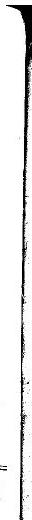
\includegraphics[max width=\textwidth]{2022_07_16_f4e476ee2159dc67e746g-32(1)}

tion on $A$, then $D$ satisfies the following four properties:

(1) $D_{x}(Y+Z)=D_{x} Y+D_{x} Z$

(2) $D_{(x+y)}(Z)=D_{x} Z+D_{y} Z$

(3) $D_{(f X)} Y=f D_{X} Y$

(4) $D_{X}(f Y)=(X f) Y+f D_{X} Y$.

These properties imply the vector $\left(D_{X} Y\right)_{m}$, at a point $m$ in $M$, depends only on $X_{m}$ and the values of $Y$ on some curve that fits $X_{m}$ For, let $e_{1}, \ldots, e_{n}$ be a $C^{\infty}$ base field about $m$, let $X{ }_{m}=\sum_{1}^{n} a_{i}(m)\left(e_{i}\right)_{m}$ and $Y=$ $\sum_{1}^{n} b_{j} e_{j}$ on the domain of the base field (intersected with domain of $Y$ ). Then
$$
\begin{aligned}
\left(D_{X} Y\right)_{m} &=\left[D_{X}\left(\Sigma b_{j} e_{j}\right)\right]_{m} \\
&=\Sigma_{j}\left[\left(X_{m} b_{j}\right)\left(e_{j}\right)_{m}+b_{j}(m) \Sigma_{i} a_{i}(m)\left(D_{e_{i}} e_{j}\right)_{m}\right] .
\end{aligned}
$$
Thus $a_{i}(m), b_{j}(m)$, and $X_{m} b_{j}$ determine $D_{X} Y$ completely if the fields $D_{e_{i}}{ }_{j}$ are known (see section 5.2).

The existence of many manifolds with connexions has been illustrated by the natural induced connexions on hypersurfaces of $R^{n}$.

Let $\sigma$ be a curve in $M$ with tangent field $T .$ A $^{\infty}$ vector field $Y$ on $\sigma$ is parallel along $\sigma$ iff $D_{T} Y=0$ on $\sigma$. The curve $\sigma$ is a geodesic iff $D_{T} T=0$ on $\sigma .$ Thus a curve is a geodesic iff its tangent field is a parallel field along the curve. The following two theorems give the existence of parallel fields and geodesics. The domain of an index of summation is always $1, \ldots, n$ unless otherwise specified.

THEOREM. Let $\sigma$ be a curve on $[a, b]$ with tansent $T$. For each vector $Y$ in $M_{\sigma(a)}$ there is a unique $C^{\infty}$ field $Y(t)$ on $\sigma$ such that $Y(a)=$ $Y$ and the field $Y(t)$ is parallel along $\sigma_{0}$ The mapping $P_{a, t} M_{\sigma(a)} \rightarrow$ $M_{\sigma(t)}$ by $P_{a, t}(Y)=Y(t)$ is a linear isomorphism which is called parallel translation along $\sigma$ from $o(a)$ to $o(t)$

\section{Section 5.1. Invariant viewpoint.}
$U$, and let $X_{1}, \ldots, X_{n}$ be the associated coordinate fields we define $C^{\infty}$ functions $\Gamma_{i}$ on $U$ by $D \quad X \quad \ldots \Gamma_{i} Y$. Wefine $\left[a, b_{1}\right]$ into $U_{0}$ If $Y(t)$ is a fietd on $\sigma$ in functions $a(t)$ on this is a field on $\sigma$ with domain $\left[a, b_{1}\right]$, then defin $x, \circ \sigma(t)$ on $[a, b]$, so $T(t)=b_{i}(t) X(\sigma(t))$, Let $g_{i}(t)=$ If $Y(t)$ is parallel along $a_{i}$, where $g_{j}^{\prime}(t)=\left(d g_{j} / d t\right)$.
$$
0=D_{T} Y=\Sigma_{i}\left[a_{i}^{\prime} X_{i}+a_{i} \Sigma_{j} g_{j}^{t} \Gamma_{i j}^{k} X_{k}\right]
$$
Thus $Y(t)$ parallel along $\sigma$ iff

(5) $\frac{d a_{k}}{d t}+\Sigma_{i, j} a_{i} \frac{d g_{j}}{d t} \Gamma_{i j}^{k}=0$

for $k=1, \ldots, n$ and for $t$ in $\left[a, b_{1}\right]$. The condition $Y(a)=Y$ defines $t$ initial values $a_{i}(a)$, and the theory of ordinary differential equation hen gives a unique set of $C^{\infty}$ functions $a_{i}(t)$, satisfying the above equations on the whole domain $\left[a, b_{1}\right]$, since the equations are line This defines the parallel field $Y(t)$.

For $t$ in $\left[a, b_{1}\right]$, the map $P_{a_{i} t}$ is linear because of the linearity of the equations $(5)$

If $t$ is any number in $[a, b]$, we obtain $P_{a, t}$ by covering the compact set $o([a, t])$ by a finite number of coordinate neighborhoods and parallel translating through each neighborhood via solutions of the systems (5)./I

THEOREM. Let $m$ be in $M, X$ in $M m^{\circ}$ Then for any real number $b$ there exists a real number $r>0$ and a unique curve $\sigma$, defined on $[b-r, b+r]$ such that $o(b)=m, T_{\sigma}(b)=X$, and $\sigma$ a geodesic.

Proof. Using the notation of the above proof, we must find $C^{\infty}$ functions $g_{i}(t)$ that satisfy the second-order differential system,

(6) $\frac{d^{2} g_{k}}{d t^{2}}+\sum_{i, j} \Gamma_{i j}^{k} \frac{d g_{i}}{d t} \frac{d g_{\mid j}}{d t}=0$ with initial conditions $g_{i}(b)=x_{i}(m)$ and $X=\Sigma g_{i}(b) X$. The theory ordinary differential equations provides us with the $r^{\prime}>0$ and the functions $g_{i}(t) . / /$

The existence and uniqueness theory of ordinary differential eq uations will actually give us much more than the conclusion of the above theorem. In particular, if we let $\sigma(t ; m, X, b)$ be the curve provided by the theorem, then the mapping $\sigma$ is actually $C^{\infty}$ with respect to all its parameters $t, m, X$ and $b$.

The torsion tensor of a connexion $D$ is a vector valued tensor Tor that assigns to each pair of $C^{\infty}$ vectors $X$ and $Y$, with domain $A$, a $C^{\infty}$ vector field $\operatorname{Tor}(X, Y)$, with domain $A$, by

(7) $\operatorname{Tor}(X, Y)=D_{X} Y-D_{Y} X-[X, Y]$

One checks easily that $\operatorname{Tor}(X, Y)=-\operatorname{Tor}(Y, X), \operatorname{Tor}(X+Y, Z)=$ $\operatorname{Tor}(X, Z)+\operatorname{Tor}(Y, Z)$, and $\operatorname{Tor}(f X, Y)=f$ Tor $(X, Y)$, where $f$ in $f$, and $Z$ in $X_{A}$. Thus the value of Tor $(X, Y)$ at a point $m$ depends only on $X_{m}$ and $Y_{m}$, and not on the fields $X$ and $Y$, by the theorem at the end of Chapter 4. If more than one connexion enters the discussion, we write Tor ${ }_{D}$ for the torsion of the connexion $D$. If Tor $_{D} \equiv 0$, then we say $D$ is symmetric, or torsion free.

As far as we know, there is no nice motivation for the word to do with the "torsion of a space curche the above tensor. In particular, it has nothing with the "torsion of a space curve".

The following definition of curvature has been motivated in secion $2.4 .$

The curvature tensor of a connexion $D$ is a linear transformation a linear transformation $R(X, Y)$ af $M$ and $Y$ at $m$ by imbedding $Y, Y_{\text {and }}$ into itself. We define $R(X, Y) Z$ inbedding $X, Y$, and $Z$ in $\mathcal{C}$ fields about $m$ and setting
$$
R(X, Y) Z=\left(D_{X} D_{Y} Z-D_{Y} D_{X} Z-D_{[X, Y} Z\right)_{m} .
$$
Again we check linearity over the ring of $C^{\infty}$ functions as coefficients on the right to determine the tensor character of $R$. Here $R(X, Y) Z=-R(Y, X) Z$, and if $f$ is $C^{\infty}$, then

\section{Notes on Differential Geometry}
$\left.R(f X, Y) Z=f D_{X} D_{Y} Z-(Y f) D_{X} Z-f D_{Y} D_{X} Z+(Y f) D_{X} Z-f D_{[x, Y}\right]^{Z}$
$$
=f R(X, Y) Z \text {. }
$$
Also
$$
\begin{aligned}
R(X, Y)(f Z)=D_{X}\left[(Y f) Z+f D_{Y} Z\right]-D_{Y}\left[(X f) Z+f D_{X} Z\right]-([X, Y] f) Z \\
&-f D_{[X, Y]} Z=(X Y f) Z+(Y f) D_{X} Z+(X f) D_{Y} Z+f D_{X} D_{Y} Z-(Y X f) \\
&-(X f) D_{Y} Z-(Y f) D_{X} Z-f D_{Y} D_{X} Z \\
&-([X, Y] f) Z-f D_{[X, Y]} Z=f R(X, Y) Z
\end{aligned}
$$
The linearity of $R(X, Y) Z$ with respect to addition (in each of its variables) is trivial to check.

The tensor nature of the torsion and curvature will again be verified in section $5.3$ with exhibition of the classical coordinate representations of these tensors.

The concept of a "connexion-preserving" map follows naturally. Let $M$ and $M^{\prime}$ be $C^{\infty}$ manifolds with connexions $D$ and $D^{\prime}$, respective A $C^{\infty}$ map $f: M \rightarrow M^{\prime}$ is connexion preserving if $f_{*}\left(D_{X} Y\right)=D_{f_{*}}\left(f_{*} Y\right)$ for all vectors $X$ and fields $Y$. Note the right side is well-defined since $f_{*} Y$ is a well-defined field on some curve that fits $f_{*} X$. A $C^{\infty}$ map $f: M \rightarrow M^{\prime}$ is geodesic preserving if $f_{\circ} g$ is a geodesic in $M^{\prime}$ for each geodesic $g$ in $M$. Trivially, a connexion-preserving map is geodesic preserving.

THEOREM. Let $f$ be a diffeomorphism of $M$ onto $M^{\prime}$, and let $D^{\prime}$ be a connexion on $M^{\prime}$. Then there is a unique connexion $D$ on $M$ for which $f$ is connexion preserving.

Proof. Take $X$ in $M_{m}$ and let $Y$ be a field about $m$. Since $f$ is a diffeo, $f_{*} Y$ is a field about $f(m)$. Define $D_{X} Y=f_{*}^{-1}\left(D_{f_{*}}^{\prime} f_{*} Y\right)$. The verification that $D$ is a connexion is left as an exercise.

If every geodesic $g(t)$ can be extended so it is a geodesic for all $t$ in $R$, then the connexion $D$ is complete.

\section{Chap. 5 Connexions}
\section{Section 5.2. Cartan viewpoint.}
For local problems concerning a connexion, one can transform the properties of $D$ to certain properties of differential forms. By using . fiber bundles associated with a manifold, one can also study global problems via differential forms. We develop the 1 ocal viewpoint here. out this section. Let $U$ be a fixed open set (perhaps a coordinate domain) in $M_{9}$ and let $e \ldots, \ldots$ be a fixed base field of independent domain) in $M_{\text {o }}$ and let e C vectors on $U$. Let $w_{1}, \ldots, w_{n}$ be the $C^{\infty}$-forms on $U$ which are the dual base to $e_{1} \ldots, e_{n}$ at each point of $U_{0}$ Define $n^{2}$ connexion if torms on $U$ which are associated with $D$ and the base field by

(9) $D_{X_{j}} e_{i=1}^{n} \sum_{i j}^{n}(X) e_{i}$

The $W_{i j}$ are linear by property (2) of the connexion $D$, and $w_{i j}$ are $C^{\infty}$, since if $X$ a $C^{\infty}$ field on $U$, then $D_{x}$ e is a $C^{\infty}$ field, so $W_{i j}(X)=$ $w_{i}\left(D_{X} e_{j}\right)$ is a $C^{\infty}$ function.

The torsion and curvature tensors may also be expressed via differential forms associated with the base field. Define 2 -forms $T$ and $R_{i j}$ on $U$ by

(10) $T(X, Y)=\sum_{i=1}^{n} T_{i}(X, Y) e_{i}$

(11) $R(X, Y) e_{j}=\sum_{i=1}^{n} R_{i j}(X, Y) e_{i}$

where the properties of an alternating tensor are checked for $T_{i}$ and $R_{i j}$ via the properties of $T$ and $R$.

The forms $W_{i}, w_{i j}, T_{i}$, and $R_{i j}$ are related by the Cartan structural equations which are equivalent to the definition of the torsion and curvature tensors. We merely express everything in terms of the base field. Let $X$ and $Y$ be $C^{\infty}$ fields on $U$. Then,
$$
T_{i}(X, Y) e_{i}=D_{X} Y-D_{Y} X-[X, Y]
$$
$$
=D_{X}\left(\Sigma_{W_{j}}(Y) e_{j}\right)-D_{Y}\left(\Sigma_{W_{j}}(X) e_{j}\right)-\Sigma_{W_{j}}([X, Y]) e_{i}
$$
Let $D$ be a connexion on an n-manifold $M$, and fix $D$ and $M$ through-
$$
\begin{aligned}
&=\Sigma\left(X_{w_{j}}(Y)-Y_{w_{j}}(X)-w_{j}[X, Y]\right) e_{j} \\
&+\Sigma\left(w_{j}(Y) w_{i j}(X)-w_{j}(X) w_{i j}(Y)\right) e_{i \cdot}
\end{aligned}
$$
Equating components,
$$
T_{i}(X, Y)-\left(\Sigma_{W_{i j}} \wedge W_{j}\right)(X, Y)=X W_{i}(Y)-Y_{W_{i}}(X)-w_{i}[X, Y] .
$$
Since the expression on the left is a 2-form, so is the expression on the right (taken as a whole), and indeed, it is the exterior derivative $d w_{i}$ of $w_{i}$ evaluated on $X$ and $Y$. With this motivation we define the exterior derivative operator $d$ on 1 -forms and functions $(0$-forms) as follows.

For a $C^{\infty}$ function $f$ with domain $A$, let $d f(X)=X f$; thus $d f$ is a $C^{\infty}$ 1-form on $A$. Let $w$ be any $C^{\infty}$ 1-form with $\operatorname{domain} A$. Then $d w$ is a $C^{\infty}$ 2-form with domain $A$, defined on $C^{\infty}$ fields $X, Y$ on $A$ by
$$
d w(X, Y)=X w(Y)-Y_{W}(X)-W[X, Y]
$$
We leave it to the reader to check that the right side is linear in each slot over the ring of $C^{\infty}$ functions on $A$, and hence that

$d w\left(X_{m}, Y_{m}\right)$ is defined for $m$ in $A$ independent of the fields $X$ and $Y$.

If $f$ is a $C^{\infty}$ function on $A$, then $d^{2} f=d(d f)=0$. To see this, let $X$ and $Y$ be $C^{\infty}$ fields on $A$; then,
$$
\begin{aligned}
d^{2} f(X, Y) &=X d f(Y)-Y d f(X)-d f[X, Y] \\
&=X Y f-Y X f-[X, Y] f=0
\end{aligned}
$$
Also note that if $x_{1}, \ldots, x_{n}$ a coordinate system on $A$, then $d x_{1}, \ldots, d x_{n}$ is the dual base to $\partial / \partial x_{1}, \ldots, \partial / \partial x_{n}$, since $d x_{i}\left(\partial / \partial x_{j}\right)=\partial x_{i} / \partial x_{j}=\delta_{i j}$ (the Kronecker delta).

Now we can write the first Cartan structural equation,

(13) $d w_{i}=-\sum_{i=1}^{n} w_{i j} \wedge w_{j}+T_{i^{*}}$

By a computation involving the definition of $R(X, Y)$, which is completely analogous to the above computation, one obtains the second

\section{Chap. 5 Connexions}
Cartan structural equation,
$$
\text { (14) } d w_{i j}=-\sum_{k=1}^{n} w_{i k} \uparrow w_{k j}+R_{i j \cdot}
$$
These equations provide an alternate proof of the tensor character of $T$ and $R$, since they show that $T_{i}$ and $R_{i j}$ are 2 -forms.


\section{Chap. 5 Connexions}


\section{Section 5.5. Bundle viewpoint.}


\begin{enumerate}
  \setcounter{enumi}{42}
  \item Let $\mathrm{x}_{1}=\mathrm{x}$ and $\mathrm{x}_{2}=y$ be the usual coordinates on $R^{2}$. Define a connexion $D$ on $R^{2}$ by letting $\Gamma_{j k}^{i} \equiv 0$ except for $\Gamma_{12}^{1}=\Gamma_{21}^{1} \equiv$ Set up and solve the differential equations for the geodesics thru any point in $R^{2}$. Find the particular geodesic $g$ with $g(0)=$ $(2,1)$ and $T_{s}(0)=(\partial / \partial x)+(\partial / \partial y)$. Is $D$ complete? Do the geodesics emanating from the origin pass thru all points of the plane? If $\sigma$ and $y$ are geodesics with $\gamma(0)=\sigma(0)$, and $T_{\gamma}(0)=b t_{\sigma}(0)$ for $b$ in $R_{\text {s }}$ show $\gamma(t)=o(b t)$ for all possible $t$ Investigate the connexion $D^{\prime}$ with all $\Gamma_{j k}^{i} \equiv 0$ except $\Gamma_{12}^{1} \equiv 1$.

  \item Let $D$ be a connexion on $M$. Let $o(t)$ be an integral curve of the $C^{\infty}$ field $X_{,}$let $e_{1}(t), \ldots$, e $(t)$ be a parallel base along $\sigma$ and let $Y(t)=\sum y_{i}(t) e_{i}(t)$ be a $C^{\infty}$ field along $\sigma .$ Show $\left(D{ }_{X} Y\right)(t)$ $\Sigma\left(d y_{i} / d t\right)_{e}(t)$ along $\sigma_{*}$ Show $\left(D_{x} Y\right)(0)=\lim (1 / t)[(P \quad Y(\sigma(t))-$ $\boldsymbol{Y}(0)]$ as $t \rightarrow 0$

  \item Let $f$ be a connexion preserving $C^{\infty}$ map of $M$ into $M^{\prime}$. Show $f_{*}($ Tor $(X, Y))=\operatorname{Tor}^{\prime}\left(f_{*} X, f_{*} Y\right)$ and $f_{*}(R(X, Y) Z)=R^{\prime}\left(f_{*} X,\right.$, $\left.f_{*} Y\right)\left(f_{*} Z\right)$

  \item A manifold $M$ is parallelizable if there is a connexion $D$ on $M$ in which parallel translation is independent of curves, and such a $D$ is called a flat connexion. Show $M$ is parallelizable iff there is a global $C^{\infty}$ base field on $M$. If $D$ is a flat connexion, show its curvature tensor is zero (see problem 85 ).

  \item Let $G$ be a Lie group. Define the left invariant connexion $D$ on $G$ by asserting all vector fields in the Lie algebra $y$ are parallel fields. Show $D$ is flat, $G$ is parallelizable, and if $X$ and $Y$ are in $S_{\text {, then }} \operatorname{Tor}(X, Y)=-[X, Y]$. Show that each geodesic $g$ on $G$ is the left translate of a one-parameter sub group $\sigma$; i.e., $g(t)=L$ s $(a)(t))$ for all $t$. Show $D$ is complete.

  \item Let $D$ be a connexion on $M$. For $m$ in $M$, let $H_{m}$ denote the set of linear maps of $M$ into itself, obtained by parallel translation of $M_{m}$ around broken $C^{\infty}$ curves starting and end ing at $m .$ Show $H$ is a group. If $M$ is connected, show $H$ is isomorphic to $H$, for $m^{\prime}$ in $M$. The group $H$ is called the holonomy group at $m$, and if $M$ is connected then the holonomy. group of $M$ is the group $H=H$, for any $m$ in $M$, Restricting group of $M$ is the group $H=H_{m}$ for any $m$ in $M .$ Restricting stricted holonomy sroup $H^{0}$ If $D$ is obtains the re$M$ is the unit sphere in $R 3^{\circ}$ If $D$ is flat, show $H_{m}=0 .$ If $M$ is the unit sphere in $R^{3}$ and $D$ is the Riemannian connexion, show that $H=S O(2, R)$, where $S O(2, R)$ is the special orthog- onal group, or rotation group, consisting of orthogonal maps with determinant one.

  \item (Continuing problem 13.) Let $X=\partial / \partial x_{1}$ and $Y=\partial / \partial x_{2}$ for $a$ coordinate system $x_{1}, \ldots, x_{n}$ on $M$ about $m$, and show $\lim _{t \rightarrow 0}(1 / t)\left[\left(P_{0, t}-I\right)\left(\partial / \partial x_{j}\right)\right]^{n}=R(Y, X)\left(\partial / \partial x_{j}\right)=\sum_{k} R_{j 2 I}^{k}\left(\partial / \partial x_{k}\right)$ where $I$ is the identity map and $P_{0, t}$ is parallel translation along $\gamma$ from $\gamma(0)$ to $\gamma(t)$. Because of this, one often says $R(X, Y)$ is "infinitesional parallel translation around an infi nitesimal parallelogram spanned by $X$ and $Y . "$

\end{enumerate}
\section{Riemannian Manifolds and Submanifolds}
The definition of a Riemannian (and a semi-Riemannian) manifold was given in section 2.1. A manifold on which one has singled qut a specific symmetric and positive definite (or non-singular) 2-covariant tensor field, called the metric tens or, is a Riemannian (or semiRiemannian) manifold. In this chapter we generalize the theory of Chapters 2 and 3 in a natural way. Much of the theory applies to semi-Riemannian manifolds and submanifolds, but, in general, we phrase things only in Riemannian terms.

\section{Section 6.1. Length and distance.}
The metric tensor allows us to define lengths, angles, and distances. Let $M$ be a Riemannian manifold with metric tensor $<$, $>$. Let $X$ and $Y$ be in $M_{m}$. Define the length of $X$ by $|X|=\sqrt{\langle X, X>}$. Define the angle $\theta$ between $X$ and $Y$ (both non-zero) by letting $\langle X, Y\rangle=|X||\boldsymbol{Y}| \cos \theta$ where $0 \leq \theta \leq \pi$, and notice the $S$ chwartz inequality $|<X, Y>| \leq$ $|X||Y|$ makes this possible.

The length of a curve is now defined by integrating the length of its tangent vector field. Let $\sigma$ be a $C^{\infty}$ curve on $[a, b]$ with tangent field $T$ (or $T_{\sigma}$ if necessary). The length of $\sigma$ from a to be, denoted by $|\sigma|_{a}^{b}$, is defined by

(1) $\quad|\sigma|_{a}^{b}=\int_{a}^{b} \sqrt{<T(t), T(t)>d t}$.

\section{Notes on Differential Geometry}
The integral exists, since the integrand is continuous. The length of a broken $C^{\infty}$ curve is defined as the (finite) sum of the lengths of its $C^{\infty}$ pieces. The number $|\sigma|_{a}^{b}$ is independeni of the parameterization of its image set in the following sense: let $g$ be a $C^{1} \operatorname{map}$ of $[c, d]$ into $[a, b]$ with end points mapping to end points (assume $g(c)=a$ and $g(d)=b) ;$ then
$$
\begin{aligned}
\int_{a}^{b}<T_{\sigma}(t)_{\nabla} T_{\sigma}(t)>^{1 / 2} d t &=\int_{c}^{d}<T_{\sigma}(g(t)), T_{\sigma}(g(t))>1 / 2 g^{\prime}(t) d t \\
&=\int_{c}^{d}<T_{\sigma_{g}}(t), T_{\sigma \circ g}(t)>^{1 / 2 d t}
\end{aligned}
$$
since $T_{\sigma \sigma_{B}}(t)=g^{\prime}(t) T_{\sigma}(g(t))$ by the chain rule. Thus we can write $|\sigma|_{\dot{q}}^{p}=|\sigma|_{a}^{b}$, where $q=\sigma(a)$ and $p=\sigma(b)$.

Classically, the metric tensor is almost always expressed by the notation "ds ${ }^{2}=g_{i j} d x_{i} d x_{j}{ }^{n}$ This means one is giving the inner product on a coordinate domain $U$ with coordinate functions $x_{1}, \ldots, x_{n}$ in terms of the coordinate bases; i.e., if $X_{i}=\partial / \partial x_{i}$, then $g_{i j}=\left\langle X_{i}, X_{j}\right\rangle$ is a $C^{\infty}$ function on $U$. If $Y=\Sigma y_{i} X_{i}$ and $Z=\sum z_{k} X_{k}$, then $\langle Y, Z>=$ $\sum_{i, k=1}^{n} y_{i} z_{k} g_{i k}$ Thus, giving the matrix of functions $g_{i j}$ on $U$ determines the inner product on $U$. The "ds" only makes sense when one is discussing a curve $\sigma$ which maps into $U$, for then let $s(t)=|\sigma|_{a}^{t}$ and
$$
\left(\frac{d s}{d t}\right)^{2}=\langle T, T\rangle=\Sigma_{i j} \frac{d\left(x_{i} \circ \sigma\right)}{d t}-\frac{d\left(x_{j} \circ \sigma\right)}{d t}
$$
If $M$ is connected, a pseudo-metric is defined on $M$ by

(2) $d(p, m)=\inf \left[|\sigma|: \sigma\right.$ a broken $C^{\infty}$ curve from $p$ to $\left.m\right] .$

Trivially, $d(p, m) \geq 0, d(p, p)=0$, and $d(p, m)=d(m, p)$. The triangle inequality is left as a problem.

THEOREM. The pseudo-metric topology on $M$ equals the manifold topology.

Proof. (After Seifert and Threlfall, p. 44). Let $m$ be any point in $M$, and let $x_{1}, \ldots, x_{n}$ be a coordinate system about $m$ with domain $U$.

\section{Chap. 6 Riemannian Manifolds and Submanifolds}
For $p$ in $U$ let $d(p)=d\left(m^{\prime}, p\right)$ defined above, and let $d^{\prime \prime}(p)=\left[\Sigma_{x_{i}}(p)^{2}\right]^{1 / 2}$ where we assume $x_{i}(m)=0$. Choose $a>0$ so $A=\left[p: d^{\prime}(p) \leq a\right]$ is contained in $U$. On the compact set $B=\left[\left(p_{1} X_{p}\right)\right.$ : $p$ in $A$ and $1=$ $\left.\Sigma d x_{i}\left(X_{p}\right)^{2}\right]$, the norm function., $\left|X_{p}\right|=\left[\Sigma_{i j} \oint_{i j}(p) d x_{i}\left(X_{p}\right) d x_{j}\left(X_{p}\right)\right]^{1 / 2}$, is a continuous function which takes on a maximum $R$ and a minimum $r>0$

Let $\sigma$ be any broken $C^{\infty}$ curve in $A$ with $\sigma(0)=m, \sigma(b)=p$ and $\left(\sigma(t), T_{\sigma}(t)\right)$ always in $B$. Then $|\sigma|=\int_{0}^{b}\left|T_{\sigma}(t)\right| d t \geq r b \geq r d^{\prime}(p)$. For a broken curve $\sigma$ from $m$ to $p$ that leaves $A$, one has $|\sigma| \geq r a \geq r d^{\prime}(p)$. Hence, $(1) d(p) \geq r d^{\prime}(p)_{\dot{d}^{\prime}}$ But if $\sigma$ curve with $x_{i} \circ \sigma(t)=\operatorname{tp}_{i} / d^{\prime}(p)$, where $x_{i}(p)=p_{i}$, then $|\sigma|=\int_{0}\left|T \sigma_{\sigma}(t)\right| d t \leq R d^{\prime}(p) .$ Hence, (2) $d(p) \leq R d^{\prime}(p)$.

The inequalities (1) and (2) prove the theorem.//

Corollary. A connected Riemannian manifold $M$ is Hausdorff iff the pseudo-metric $d$ is a metric.

In Chapter 10 we show that geodesics are the curves that locally minimize arc length, i.e., the length of a small piece of a geodesic in $M$ is precisely the distance between the end points of the piece.

Henceforth we assume all manifolds we mention are Hausdorff. A Riemannian manifold is complete if it is complete as a metric space, i. e., every Cauchy sequence must converge.

Section 6.2. Riemannian connexion and curvature.

A Riemannian connexion $D$ on a Riemannian manifold $M$ is a connexion $D$ such that

(3) $D_{X} Y-D_{Y} X=[X, Y]_{1}$ and

(4) $Z\langle X, Y\rangle=\left\langle D_{Z} X_{,} Y\right\rangle+\left\langle X, D_{Z} Y\right\rangle$

for all fields $X, Y$, and $Z$ with a common domain. The fundamental theorem of (semi-) Riemannian manifolds is the following:

THEOREM. There exists a unique Riemannian connection on a (semi-) Riemannian manifold.

Proof. We show a Riemannian connexion $D$ exists and is unique on every coordinate domain $U$. The uniqueness implies $D$ must agree on overlapping domains; hence $D$ exists and is unique on all of $M$.

Let $X_{1}, \ldots, X_{n}$ be the coordinate fields on $U$, let $g_{i j}=\left\langle X_{i}, X_{j}\right\rangle$ on $U$, and let $\left(g^{-1}\right)_{i j}$ be the $j^{\text {th }}$ entry of the inverse matrix of $g=\left(g_{i j}\right)$ (which is non-singular). If (3) and (4) hold, then
$$
X_{i}\left\langle X_{r^{\prime}}, X_{j}>+X_{j}\left\langle X_{r}, X_{i}>-X_{r}\left\langle X_{i}, X_{j}\right\rangle=2\left\langle D_{X_{i}} X_{j}, X_{r}>\right.\right.\right.
$$
since $\left[X_{k}, X_{s}\right]=0$ for all $k$, s. By section $5.2$, giving $D$ on $U$ is equivalent to giving functions $\Gamma_{i k}^{i}$ with $D_{X}\left(X_{j}\right)=\sum_{i=1}^{n} \Gamma_{i k}^{i} X_{i}$ and demanding properties (1) through (4) of section $5.1$ are valid. Thus (5) implies $2 \Sigma_{k} \Gamma_{j i}^{k} g_{k r}=X_{j} g_{r j}+X_{j} g_{t i}-X_{r} g_{i j}$; hence

(6) $\quad \Gamma_{i j}^{k}=1 / 2 \Sigma_{r}\left(g^{-1}\right)_{k f}\left(\frac{\partial g_{r j}}{\partial x_{i}}+\frac{\partial g_{r i}}{\partial x_{j}}-\frac{\partial g_{i j}}{\partial x_{r}}\right)$

This is the classical expression for the Christoffel function $\Gamma_{i j}^{k}$ in terms of the metric tensor. Use (6) to define $D$ on $U$. A direct check of (3) and (4) shows $D$ is Riemannian, and the explicit representation (6) shows $D$ is unique. I/

The above theorem is special case of a more general theorem (problem 70). For the rest of this section let $M$ be a (semi) Riemannian manifold and let $D$ be the Riemannian connexion on $M$. The Riemann-Christoffel curvature tensor (of type 0,4 ) is the 4-covariant tensor $K(X, Y, Z ; W)=\left\langle X, R(Z, W) Y>\right.$ for $X, Y, Z$, and $W$ in $M_{m}$

THEOREM. The following relations are true:

(a) $R(X, Y) Z+R(Z, X) Y+R(Y, Z) X=0$

(b) $K(X, Y, Z, W)=-K(Y, X, Z, W)$

(c) $K(X, Y, Z, W)=-K(X, Y, W, Z)$

(d) $K(X, Y, Z, W)=K(Z, W, X, Y)$

The relation (a) is called the first Biachi identity and it holds for any symmetric connexion. These relations are equivalent to the "symmetries" of the indices of the classical $R_{i j k h}$ functions.

Proof. For (a), use the Jacobi identity, property (3) above, and compute. For (c), use $R(Z, W)=-R(W, Z)$. For (b), use property (4) to shift $D$ from one slot to the other. For (d), notice (a) implies $\left(a^{\prime}\right)$ : $K(X, Y, Z, W)+K(X, W, Y, Z)+K(X, Z, W, Y)=0 .$ By writing (a') three more times, cyclicly permuting the arguments of the first term one step from one line to the next, adding all four equations, and cancelling via (b) and (c), one obtains (d).//

For $X$ and $Y$ in $M_{m}$, let

(7) $A(X, Y)=\left\langle X, X>\left\langle Y, Y>-\left\langle X, Y>^{2}\right.\right.\right.$.

If $A(X, Y) \neq 0$, let

(8) $\bar{K}(X, Y)=K(X, Y, X, Y) / A(X, Y)$

and by direct computations, using the above properties of $K_{\text {, one }}$ can show
$$
\bar{K}(X, Y)=\bar{K}(Y, X)=\bar{K}(r X, s Y)=\bar{K}(X+t Y, Y)
$$
for $r, s$, and $t$ not $z$ ero. Thus if $A(X, Y) \neq 0$ and ad $-b c \neq 0$, then $\bar{K}(X, Y)=\bar{K}(a X+b Y, c X+d Y)$, and we define $K(P)$, the Riemannian curvature of the 2-dimensional subspace $P$ of $M_{m}$ spanned by $X$ and $Y$, by $K(P)=\langle X, R(X, Y) Y>/ A(X, Y)$. In section $2.4$, we showed $\boldsymbol{K}\left(M_{m}\right)=K(m)$ is the Gauss curvature of a surface $M$ in $R^{3}$. In the Riemannian case, $[A(X, Y)]^{1 / 2}$ is the area of the parallelogram spanned by $X$ and $Y$.

Let $f: M \rightarrow M^{\prime}$ be a $C^{\infty}$ map between Riemannian manifolds. If there is a $C^{\infty}$ real valued positive function $F$ on $M$ such that for all $m$ in $M$ and all $X, Y$ in $M_{m},\left\langle f_{\dot{*}} X, f_{*} Y\right\rangle=F(m)\langle X, Y\rangle$, then $f$ is a conformal (or strictly conformal) map and $F$ is called the scale function. If $F$ exists but $F \geq 0$ only, then $f$ is weakly conformal. If $F=1$, then $f$ is an isometry. If $f$ is an isometry and a liffeomorphism, then $f$ is isometric and $M$ is isometric to $M^{\prime}$. If $F$ is constant, then $f$ is homothetic.

At this point, we explicitly call the reader's attention to problem 52, which is considered an integral part of the theory of Riemannian manifolds.

\section{Notes on Differential Geometry}
\section{Section 6.3. Curves in Riemannian manifolds.}
This section parallels the standard treatment of curves in advanced calculus. Let $M$ be a Riemannian manifold with Riemannian connexion $D$. Let $\sigma$ be a $C^{\infty}$ curve in $M$ with tangent field $V=\sigma_{*}(d / d t)$, which can legitemately be called the "velocity vector" of $\sigma$ since "length" is defined. Assuming $V$ does not vanish on the domain of $\sigma$, define the unit tangent vector $T(t)=V(t) /|V(t)|$, and define the speed function $s^{\prime}=(d s / d t)=|V(t)|$, so $V(t)=s^{\prime}(t) T(t)$ for $t$ in the domain of $\sigma$. Define the geodesic curvature vector field of $\sigma$ to be the field $D_{T} T$, and its length $k_{1}$ is the geodesic curvature of $\sigma_{0}$ Notice that $D_{T} T$ and $k_{1}$, at a particular point on the curve, do not depend on the parameterization of the "point set of the curve" but only on the orientation (choice of "direction") and the existence of a $C^{\infty}$ parameterization with non-vanishing tangent at the point.

The curve $\sigma$ is a geodesic $\left(D_{V} V=0\right)$ iff $V$ has constant length and (a) $D_{T} T=0$ or $(\mathrm{b}) k_{1}=0$. This follows $\operatorname{since} D_{V} V=s^{\prime} D_{T}\left(s^{\prime} T\right)=$ $s^{\prime} s^{\prime \prime} T+\left(s^{\prime}\right)^{2} D_{T} T$ and $s^{\prime}>0$ while $D_{T} T$ is orthogonal to $T,(<T, T>=$ 1 so $\left.0=T<T, T\rangle=2<D_{T} T, T>\right)$.

When $k_{1}(t)>0$, define the (first) normal to $\sigma$ at $\sigma(t)$ to be the unit vector $N_{1}(t)$ such that $D_{T} T=k_{1} N_{1}$ at $t$. If $N_{1}$ is defined on an interval, then, $0=T\left\langle N_{1}, T\right\rangle=\left\langle D_{T} N_{1}, T\right\rangle+\left\langle N_{1}, D_{T} T\right\rangle=\left\langle D_{T} N_{1}, T\right\rangle+k_{1}$, so $D_{T} N_{1} \neq 0$ on the interval. The vector $D_{T} N_{1}+k_{1} T$ is orthogonal to both $T$ and $N_{1}$; hence, let its length be $k_{2}$, the second curvature or torsion. If $k_{2}(t)>0$, define the second normal to $\sigma$ at $o(t)$ to be the unit vector $N_{2}(t)$ such that $D_{T_{1}} N_{1}+k_{1} T=k_{2} N_{2} .$ If $k_{2}>0$ on an interval, then the above process can be continued to define $k_{3}$, and where $k, 0$, one gets $N$ etc. The vectors $T, N, N$ are called $F$ renet vectors, and the equations that express the $D_{T} N_{i}$ in terms of the Frenet vectors are called the Frenet formulae.

When $M$ is a 2-manifold and $k_{1}>0$, then the Frenet formulae become $D_{T} T=k_{1} N$ and $D_{T_{1}} N_{1}=-_{1} T$. In this case it is possible to locally choose $N_{1}$ along $\sigma$ independently of $D_{T} T$ (on univalent pieces of $\sigma$ ), and letting $D_{T} T=k_{1} N_{1}$ would define $k_{1}$, which could take on negative values (see problem 72 ).

\section{Chap. 6 Riemannian Manifolds and Submanifolds}
\section{Section 6.4. Submanifolds.}
The theory in sections 2,3 and $2.4$ is now generalized. Throughout this section let the $k-m a n$ ifold $M$ be a (non-singular) submanifold of the (semi-) Riemannian manifold $\vec{M}$. In the semi-Riemannian case, the submanifold $M$ is non-singular if the metric tensor is non-singular when restricted to $M_{m}$ for all $m$ in $M$ (thus $M$ is a semi-Riemannian manifold under the induced metric tensor). The induced metric tenmar on $M$ is called the first fundamental form on $M$. thet $\bar{D}$ be the sor on $M$ is called the first $f t$

THEOREM, For $C^{\infty}$ fields $X$ and $Y$ with domain $A$ on $M$ (and tangent to $M$ ), define $D_{X} Y$ and $V(X, Y)$ on $A$ by decomposing $\bar{D}_{X} Y$ into its unique tangential and normal components, respectively; thus,

(9) $\bar{D}_{X} Y=D_{X} Y+V(X, Y)$

Then $D$ is the Riemannian connexion on $M$ and $V$ is a symmetric vector-valued 2-covariant $C^{\infty}$ tensor called the second fundamental tensor. The decomposition equation (9) is called the Gauss equation.

Proof. We will establish the $C^{\infty}$ nature of the decomposition. The rest of the proof will only be outlined, for it is a simple exercise. Use the properties of $\bar{D}$ (since it is a connexion) to establish the properties of $D$ (making it a connexion) and the tensor character of $V$ (its multilinearity). Zero torsion for $\bar{D}$ implies zero torsion for $D$, and $V$ is symmetric (use the proposition in section 2.2, which generalizes trivially). Since $\bar{D}$ satisfies condition (4) (section 6.2), $D$ does too. Hence $D$ is Riemannian, and by the uniqueness theorem, $D$ is the Riemannian connexion on $M .$

To show $D$ and $V$ are $C^{\infty}$ on $A$, choose $p$ in $A$. Let $\bar{U}$ and $U$ be special coordinate domains about $p$ in $\bar{M}$ and $M$, respectively, with $U \subset A_{s}$ and let $\bar{Z}_{1}, \ldots, \bar{Z}_{n}$ and $Z_{1}=\left.\bar{Z}_{1}\right|_{U}, \ldots, Z_{k}=\left.\bar{Z}_{k}\right|_{U}$ be the coordi nate vector fields on $\bar{U}^{n}$ and $U$, respectively. Apply the Gram-Schmidt process to $\bar{Z}_{1}, \ldots, \bar{Z}_{n}$ on $\bar{U}$ to obtain $C^{\infty}$ (the Gram-Schmidt process is algebraic) orthonormal fields $W_{1}, \ldots, W_{n}$ on $\bar{U}$ such that $\left.W_{1}\right|_{U} \ldots,\left.W_{k}\right|_{U}$ give a $C^{\infty}$ orthonormal base of $M_{m}$ for $m$ in $U_{,}$while $\left.W_{k+1}\right|_{U}, \ldots,\left.W_{n}\right|_{U}$ give $\bar{M}$-vector fields that are $C^{\infty}$ on $U$ and form a base of the orthogonal complement to $M$, for $m$ in $U$. Let $X=\sum_{i=1}^{k} \times W$ and $Y=$ $\sum_{i=1}^{k} y_{j} W_{j}$ define $C^{\infty}$ functions $x_{i}$ and $y_{i}$ on $U$ for $i=1, \ldots ., k$, and let

\section{Notes on Differential Geometry}
$\widetilde{D}_{W_{i}} W_{j}=\sum_{r=1}^{n} B_{j i}^{r} W_{f}$ define $C^{\infty}$ functions $B_{i j}^{r}$ on $\bar{U}$. Then
$$
\bar{D}_{X} Y=\Sigma\left(X Y_{j}\right) W_{j}+\Sigma y_{j} B_{j i}^{r} W_{r}
$$
where $i$ and $j=1, \ldots, k$ and $t=1, \ldots, n$; thus
$$
D_{X} Y=\Sigma_{r=1}^{k}\left[\left(X_{y_{r}}\right)+\sum_{i, j=1}^{k} y_{j} x_{i} B_{j i}^{r}\right] W_{r}
$$
and
$$
V(X, Y)=\sum_{t m k+1}^{n}\left[\sum_{i, j=1}^{k} y_{j} x_{i} B_{j i}^{r}\right] W_{r}
$$
are $C^{\infty}$ on $U . / /$

By decomposing the curvature $\bar{R}$ into tangent and normal parts, we obtain the Gauss curvature equation (10), and the Codazzi-Mainardi equation (11), respectively. Let $X, Y$, and $Z$ be $C^{\infty}$ fields tangent to $M$ with a common domain. Writing the decomposition of a vector $W$ as $W=\tan W+$ nor $W$,

(10) $\tan \bar{R}(X, Y) Z=R(X, Y) Z+\tan \left[\bar{D}_{X} V(Y, Z)-\bar{D}_{Y} V(X, Z)\right]$,

and

(11) nor $\bar{R}(X, Y) Z=V\left(X, D_{Y} Z\right)-V\left(Y, D_{X} Z\right)-V([X, Y], Z)$
$$
+\operatorname{nor}\left[\bar{D}_{X} V(Y, Z)-\bar{D}_{Y} V(X, Z)\right] \text {. }
$$
Since $V$ is a tensor, i.e., $V\left(X_{m}, Y_{m}\right)$ is well-defined and independent of the fields $X$ and $Y$ used to compute it in the Gauss equation, we define $X$ and $Y$ to be conjugate vectors at $m$ if $V(X, Y)=0$. A vector $X$ in $M_{m}$ is an asymptotic vector if $V(X, X)=0$, and in any case, define the asymptotic (or normal) curvature of $X, k_{X}$, by $k_{X}=$ $|V(X, X)|$. If $V_{m}=0$, then $m$ is a flat point on $M$.

If $\sigma$ is a curve in $M$ with $C^{\infty}$ unit tangent $T$, then $V(T, T)$ is the normal curvature vector field of $\sigma$ and $k_{T}=|V(T, T)|$ is the normal curvature of $\sigma$.

\section{Chap. 6 Riemannian Manifolds and Submanifolds}
THEOREM (Meusnier). All curves on $M$ with the same unit tangent $T$ at a point have the same normal curvature at that point. If $\sigma$ a curve on $M$ with $C^{\infty}$ unit tangent $T$, then $\left(\bar{k}_{1}\right)^{2}=\left(k_{1}\right)^{2}+\left(k_{T}\right)^{2}$ relates the geodesic curvatures $\bar{k}_{1}$ and $k_{1}$ of $\sigma$ in $\bar{M}$ and $M$ with its normal curvature $k_{T}$. Moreover, $k_{T}=\vec{k}_{1} \cos \phi$ determines the angle $\phi$ between the normal $\bar{N}_{1}$ of $\sigma$ in $\vec{M}$ and the normal curvature vector $V(T, T)$ if $\phi$ is defined.

Proof. The first sentence follows since $V$ is a tensor. The second sentence follows from the Gauss equation $\bar{D}_{T} T=D_{T} T+V(T, T)$ since the vectors on the right are orthogonal. For the third sentence, if $\vec{k}_{1}=0$, then $k_{1}=k_{T}=0$ and $\phi$ not defined. If $\bar{k}_{1}>0$ and $k_{T}=0$, then $V(T, T)=0, N_{1}$ is tangent to $M$, and $\phi=\pi / 2$ (if anything). If $k_{T} \neq 0$, let $N$ be the unit normal in direction of $V(T, T)$ and
$$
k_{T}=\langle V(T, T), N\rangle=\left\langle\bar{D}_{T} T, N\right\rangle=\bar{k}_{1} \cos \phi \cdot / /
$$
The theorem and corollary at the end of section $2.3$ can now be generalized by replacing $R^{n}$ by $\bar{M}$.

\section{Section 6.5. Hypersurfaces.}
In this section, let $M$ be a hypersurface in the Riemannian manifold $\vec{M}$ and let $N$ be a $C^{\infty}$ unit normal on $M$. Define the Weingarten $\operatorname{map} L(X)=\bar{D}_{X} N$ for $X$ in $M_{m}$ (as in section 2.2). The Gauss equation for $M$ now becomes
$$
\vec{D}_{X} Y=D_{X} Y-\langle L X, Y>N
$$
$\left.\operatorname{since}\left\langle V\left(X_{9} Y\right), N\right\rangle=\left\langle\vec{D}_{X} Y, N\right\rangle=X<N, Y\right\rangle-\langle Y, L(X)\rangle$ and $\langle N, Y\rangle=0$. Thus $V(X, Y)=-\langle L, Y>N$.

The fundamental forms and the imbedded geometric invariants of $M$ in $\vec{M}$ are defined in terms of $L$ exactly as in section $2.2$. Notice in this case $V$ is symmetric is equivalent to $L$ being self adjoint.

The Gauss curvature equation (10) and Codazzi-Mainardi equation (11) now become

(13) $\tan \bar{R}(X, Y) Z=R(X, Y) Z-[\langle L Y, Z\rangle L(X)-\langle L X, Z>L(Y)]$ and

(14) nor $\bar{R}(X, Y) Z=-\left\langle D_{X} L Y-D_{Y} L X-L[X, Y], Z>N\right.$

respectively.

The torsion tensor is generalized by defining for any $C^{\infty}$ linear transformation valued tensor $W_{p}: M_{p} \rightarrow M_{p}$, on a $C^{\infty}$ manifold $M$, the torsion of $W$, Tor $_{W}$, by
$$
\operatorname{Tor}_{W}(X, Y)=D_{X} W(Y)-D_{Y} W(X)-W[X, Y] .
$$
The Codazzi-Mainardi equation (14) on a hypersurface becomes nor $\bar{R}(X, Y) Z=-\operatorname{Tor}_{L}(X, Y), Z>N . \quad$ Thus Tor ${ }_{L}=0$ on $M$ iff
$$
\bar{R}(X, Y) Z=R(X, Y) Z-[\langle L Y, Z>L X-\langle L X, Z>L Y] .
$$
The following theorem generalizes the "theorema egregium" of Gauss, and actually, it may be generalized to the case where $M$ is a $k-$ Submanifold of $\bar{M}$ (see Hicks ${ }^{1}$ ).

THEOREM. Let $M$ be a hypersurface in the Riemannian $\bar{M}$, let $P$ be a 2-dimensional subspace of $M_{m}$, and let $K(P)$ and $\bar{K}(P)$ be the Riemannian curvature of $P$ in $M$ and $M$ respectively. Let $N$ be a unit $C^{\infty}$ normal on a neighborhood of $m$, and let $L(X)=\bar{D}_{X} N$ for $X$ in $M_{M^{*}}$ If $X$ and $Y$ form an orthonormal base of $P$, then
$$
\bar{K}(P)=K(P)-\left(\langle L Y, Y\rangle\langle L X, X\rangle-\langle L X, Y\rangle^{2}\right) .
$$
Proof. Combine the definition of Riemannian curvature with the Gauss curvature equation (13).//

When $\bar{M}$ is a 3-manifold, the above theorem shows the determinant of $L$ is independent of the imbedding (i.e., independent of $L$ ) but depends only on the Riemannian structure of $\bar{M}$ and $M$.

A related result is a form of the Lemma of Synge.

THEOREM. Let $k>1$, and let $M$ be a $k-s u b m a n i f o l d$ of the Riemannian n-manifold $M$. Let $g$ be a geodesic of $M$ that lies in $M$, let $T$ be the unit tangent to g, let $X$ be a unit field tangent to $M$ which is parallel in $M$ along $g$ and orthogonal to $T$, and let $P$ be the subspace spanned by $X$ and $T$. Then $\bar{K}(P) \geq K(P)$ along $g$, and $\bar{K}(P)=K(P)$ iff $X$ is parallel along $g$ in $\bar{M}$.

Proof. We prove the theorem for $k=n-1$, leaving the other cases to problem 55. Let $N$ be a $C^{\infty}$ unit normal on a neighborhood of a point on $g$ and let $L(Z)=\bar{D}_{Z} N$. Here $\bar{D}_{T} T=0$ so $D_{T} T=0$ and $\left\langle L T, T>=0\right.$. By the previous theorem, $\left.K(P)=K(P)+\langle L X, T\rangle^{2}\right\rangle$ $K(P)$. If equality holds, then $\langle L X, T\rangle=0$ so $\bar{D}_{T} X=D_{T} X=0$, and conversely.//

There is a basic "rigidity" theorem for hypersurfaces of $R^{n}$ which is our next goal. This theorem is a uniqueness theorem, and there is a corresponding existence theorem that is proved in Chapter $9 .$ When $n=3$, the theorem was first proved by 0 . Bonnet (1867).

Intuitively, this theorem states if two hypersurfaces in $R^{n}$ are isometric and their normal $\mathrm{s}$ are "bending the same", then by a "rigid motion" one can superimpose the two manifolds.

THEOREM. Let $M$ and $M^{\prime}$ be connected hypersurfaces in $R^{n}$ for $n \geq 3$. Let $N$ and $N^{\prime}$ be $C^{\infty}$ unit normal fields on $M$ and $M^{\prime}$, respectively. Let $F$ be a diffeomorphism of $M$ onto $M^{\prime}$ that preserves the first and second fundamental forms. Then there is an isometry $G$ of $R^{n}$ with $F=\left.G\right|_{M}$

Proof. During this proof let us use "primes" to denote concepts belonging $M^{1}$ which correspond to familiar concepts for $M ;$ i.e., 1 et $L(X)=\bar{D}_{x} N$ for $X$ in $M$ and $L^{\prime}(Y)=\bar{D}_{Y} N^{\prime}$ for $Y$ in $M_{p}^{1}$. The hypothesis states if $X$ and $Z$ are in $M$, then
$$
\left\langle F_{*} X, F_{*} Z\right\rangle=\langle X, Z\rangle \text { and }\left\langle L^{\prime}\left(F_{*} X\right), F_{*} Z\right\rangle=\langle L X, Z\rangle .
$$
Combining these statements,
$$
\left\langle L^{\prime}\left(F_{*} X\right), F_{*} Z\right\rangle=\left\langle L X, Z>=\left\langle F_{*} L X, F_{*} Z\right\rangle\right.
$$
for all $Z$ which implies $L^{\prime} \circ F_{*}=F_{*} \circ L_{*}$ Thus the hypothesis could be rephrased as a demand that $F$ be an isometry of $M$ onto $M^{\prime}$ whose Jacobian commutes with the Weingarten maps. Since an isometry is

\section{Notes on Differential Geometry}
connexion preserving, $F_{*}\left(D_{X} Z\right)=D_{F}^{\prime}{ }_{*} F_{*} Z$ for vectors $X$ and fields $Z$ tangent to $M$.

If $p$ in $M$, we extend the Jacobian of $F$ to be a linear map of $\left(R^{n}\right)_{p}$ onto $\left(R^{n}\right)_{p^{\prime}}$ where $p^{\prime}=F(p)$. Let $W$ be in $\left(R^{n}\right)$, then $W=W,+a N$ where $W_{t}$ is tangent to $M$, so define
$$
F_{*}(W)=F_{*}\left(W_{t}\right)+a N_{p}^{\prime}
$$
If $X$ is in $M_{p}$ and $W$ is a $C^{\infty}$ field of $R^{n}$-vectors on $M$, then
$$
F_{*}\left(\bar{D}_{X} W\right)=\bar{D}_{F_{*}}\left(F_{*} W\right)
$$
where $\bar{D}$ is a natural covariant differentiation on $R^{n}$. This follows\\
since since
$$
\begin{aligned}
\bar{D}_{X} W &=\bar{D}_{X} W_{t}+\bar{D}_{X}(a N) \\
&=D_{X} W_{t}-<L X, W_{t}>N+(X a) N+a L X
\end{aligned}
$$
and
$$
\begin{aligned}
F_{*}\left(\bar{D}_{X} W\right) &=D_{F}^{\prime}{ }_{*} F_{*}{ }_{*}{ }_{t}-\left\langle F_{*} L X, F_{*} W_{t}>N^{\prime}+F_{*} X\left(a \circ F^{-1}\right) N^{\prime}+\left(a \circ F^{-1}\right) L^{\prime} F_{*}\right.\\
&=\bar{D}_{F *} F_{*} W_{t}+\bar{D}_{F}\left(\left(a \circ F^{-1}\right) N^{\prime}\right)=\bar{D} F_{*} F_{*}
\end{aligned}
$$
$$
\begin{aligned}
& =\bar{D}_{F_{*}} F_{*} W_{t}+\bar{D}_{F * X}\left(\left(a \circ F^{-1}\right) N^{\prime}\right)=\bar{D}_{F}, F_{*} W \text {. }
\end{aligned}
$$
Now let $e_{1}, \ldots, e_{n}$ be the usual orthonormal fields on $R^{n}$ and define $C^{\infty}$ functions $b_{r s}$ on $M$ by $F_{*}\left(e_{s}\right)_{p}=\sum_{t=1}^{n} b_{t s}(p)\left(e_{r}\right)_{p}$. The functions ${ }_{r s}$ are $C^{\infty} \operatorname{since} F, M$, and $M^{\prime}$ are $C^{\infty}$, and the $n$ by $n$ matrix $b$ (p) is orthogonal since $F$ is an isometry. Then for any tangent vector $X$ to $M$ at any point $p$ in $M$, we know $D_{X} e_{s}=0$, since $e_{s}$ are parallel fields on $R^{n}$. Thus,
$$
0=F_{*}\left(\bar{D}_{X} e_{s}\right)=\bar{D}_{F_{*} X}\left(F_{*} e_{s}\right)
$$
$=\Sigma_{r=1}^{n}\left[\left(X b_{r s}\right) e_{r}+b_{r s} \bar{D}_{F}{ }_{*} \mathrm{e}_{r}\right]=\Sigma_{r}\left(X b_{r s}\right) e_{r^{\prime}}$

\section{Chap. 6 Riemannian Manifolds and Submanifolds}
so $X b_{s_{s}}=0$ for all $r$ and s. Since $X$ and $p$ were arbitrary and $M$ is connected, the functions $b_{r s}$ are constant on $M$ and thus the Jacobian of $F$ is a constant orthogonal transformation relative to the natural base $e_{1}, \ldots, e_{n}$ of $R^{n}$

Next define a map $G$ of $R^{n}$ onto itself which is a translation followed by an orthogonal map by letting $G(p)=p^{\prime}=F(p)$ for one $p$ in $M$ and requiring $\left(G_{*}\right)_{p}=\left(F_{*}\right)_{p}$. This completely determines $G$ and the Jacobian of $G$ is constant and hence equal to the Jacobian of $F$ at all points. Since $M$ is connected, $F=\left.G\right|_{M^{*}} / /$

Section 6.6. Cartan viewpoint and coordinate viewpoint.

In this section let $M$ be a hypersurface of a Riemannian $n$-manifold $\vec{M}$. Let $p$ be in $M$, let $\bar{U}$ be a special coordinate neighborhood of $p$ in

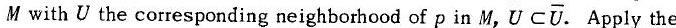
\includegraphics[max width=\textwidth]{2022_07_16_f4e476ee2159dc67e746g-44}\\
Gram-Schmidt process to the coordinate vector fields on $\bar{U}$ to obtain an orthonormal base field $e_{1}, \ldots, e_{n}$ on $\vec{U}$ with $e_{1}(m), \ldots, e_{n-1}(m)$ a base of $M_{m}$ for $m$ in $U$ and $e_{n}(m)$ normal to $M_{m}$ (thus $e_{n}$ provides a local normal for the neighborhood $U)$. Let $f: U \rightarrow \bar{U}$ be the inclusion map.

Applying the results of section $5.2$, let $\bar{w}_{1}, \ldots, \bar{w}_{n}$ be the dual 1forms associated with $e \ldots, e_{1}$ and let $\bar{W}_{i j}$ for $1 \leq i_{g} j \leq n$ be the con nexion 1-forms associated with the Riemannian connexion $\bar{D}$ on $\bar{U}$, so
$$
\bar{D}_{x} e_{j}=\sum_{i=1}^{n} \bar{w}_{i j}(X) e_{i}
$$
for $j=1, \ldots, n$.

Let $w_{i j}=\left.\bar{W}_{i j}\right|_{U}$ and $w_{i}=\left.\vec{W}_{i}\right|_{U}$ for $1 \leq i, j \leq n$, i.e., $W_{i j}=f * \bar{W}_{i j}$ $w_{i}=f^{*} \bar{w}_{i}$. Then, if $X$ is tangent to $M$ at $m$ in $U$, by the Gauss equation,

(19) $D_{X} \mathrm{e}_{j}=\sum_{i=1}^{n-1} \bar{w}_{i j}(X) e_{i}$

(20) $V\left(X, e_{j}\right)=\bar{w}_{n j}(X) e_{n}$

for $j=1, \ldots, n-1$. Thus $w_{i j}$ for $i, j \leq n$ are the connexion forms for the induced Riemannian connection $D$ on $M$. Moreover,

\section{Notes on Differential Geometry}
$$
L(X)=\vec{D}_{X} e_{n}=\sum_{i=1}^{n-1} w_{i n}(X) e_{i}
$$
since $L(X)$ in $M_{m}$, so $w_{n n}=0$ on $U$. Also $w_{n}=0$ on $U$, since $e_{n}$ is normal to $M$. Equation (18) is the Gauss equation and equation (21) is the Weingarten equation.

Let I, II, III be the first, second, and third fundamental forms, respectively. Then for $X$ and $Y$ in $M_{m}, m$ in $U$,
$$
I(X, Y)=\sum_{1}^{n-1} W_{i}(X) W_{i}(Y)
$$
$$
\begin{aligned}
& I I(K, Y)=\langle L X, Y\rangle=\sum_{1}^{n-1} W_{i n}(X) W_{i}(Y)
\end{aligned}
$$
$$
I I(X, Y)=\langle L X, L Y\rangle=\sum_{1}^{n-1} W_{i n}(X) W_{i n}(Y)
$$
Notice $0=X\left\langle e_{i}, e_{j}\right\rangle=\left\langle D_{X} e_{i}, e_{j}\right\rangle+\left\langle e_{i}, D_{X} e_{j}\right\rangle=w_{i i}(X)+w_{i j}(X)$ for all $X$ tangent to $M$, i.e. $w_{j i}=-_{i j}$ for connexion forms belonging to an orthonormal base (and this again shows $w_{n n}=0$ ). Thus we can write II and III in terms of $w_{n i}$ if we wish.

Certain relations are implied by the Cartan structural equations The equation $d \bar{W}_{n}=-\sum_{j=1}^{n} \bar{W}_{n j} \wedge \bar{W}_{j}=0$ (on $M_{m}$ ) implies II is symmetric. The equation $d \bar{w}_{n n}=-\sum_{j=1}^{n} \bar{W}_{n j} \wedge \bar{W}_{j n}=0$ (on $M_{m}$ ) implies III is symmetric, For $\dot{i}^{\prime} j \leq n_{,} d_{i j}=-\sum_{s * 1}^{n} \bar{W}_{i s} \wedge \bar{W}_{s j}+\bar{R}_{i j}$ when restricted to vectors on $M_{m}$, gives $f * d W_{i j}=d w_{i j}=-\sum_{s=1}^{n-1} W_{i s} \wedge W_{s j}+R_{i j}=$ $-\sum_{s=1}^{n} W_{i s} \wedge W_{s j}+\bar{R}_{i j}$. Thus
$$
R_{i j}=-W_{i n} \wedge W_{n j}+\bar{R}_{i j}
$$
which is the Gauss curvature equation from this point of view. For $i \leq n$
$$
f^{*} d \bar{w}_{i n}=d w_{i n}=-\sum_{s=1}^{n-1} w_{i s} \wedge W_{s n}+\bar{R}_{i n}
$$
is the Codazzi-Mainardi equation.

For the coordinate viewpoint, let $x_{1}, \ldots, x_{n}$ be the special coordinate system on $\vec{U}$ such that $x_{1}, \ldots, x_{n-1}$ give coordinates on $U$. Let $X_{i}=$ $\partial / \partial x_{i}$ for $i=1, \ldots, n-1$ and let $X_{n}=e_{n}$ the unit normal (on $U$ ). Now apply the above analysis to the base field $X_{1}, \ldots, X_{n}$ (and this time

\section{Chap. 6 Riemannian Manifolds and Submanifolds}
$W_{i j} \neq-W_{j i}$ necessarily, since the base $X_{1}, \ldots, X_{n}$ is not necessarily orthonormal).

Section 6.7. Canonical spaces of constant curvature.

We exhibit the three classical examples of $n$-dimensional $(n \geq 2)$ simply connected complete spaces with constant Riemannian curvature $K=0, K>0$, and $K<0$; i.e., the Riemannian curvature $K(P)$ of all plane sections is a constant.

For $K=0$, let $M=R^{n}$ with the usual Riemannian metric. This is usually called Euclidean space or flat space.

For $K>0$, let $M=\left[a\right.$ in $\left.R^{n+1}: \quad \sum_{1}^{n+1} a_{i}^{2}=1 / K\right]$, i. e., $M$ is the $n$ dim sphere of radius $1 / \sqrt{K}$ about the origin in $R^{n+1}$. It is a Riemannian manifold via the induced metric from $R^{n-1}$. This is called spherical space or Riemann space. Letting $N$ be the unit outer normal on $M$, then $L(X)=\sqrt{ } K X$ for all vectors tangent to $M$ and all points are umbilic. By equation (17) above, $K(P)=\langle L X, X\rangle\langle L Y, Y\rangle=K$ where $X$ and $Y$ are unit orthogonal vectors spanning $P$. Since $M$ is compact, it is complete. An alternate proof that $M$ has constant curvature is provided by the group of orthogonal tranformations on $R^{n+1}$, which provides isometries that will map any point $m$, and plane section $P$ at $m$, into any other point $m^{\prime}$ and plane section $P^{\prime}$. Since an isometry preserves the curvature, this would show $M$ has constant Riemannian curvature but would not evaluate this constant.

For $K<0$, let $M=\left[a\right.$ in $\left.R^{n}: \quad \sum_{1}^{n} a_{i}^{2}<-4 / K\right]$. Let $x_{1}, \ldots, x_{n}$ be the usual coordinate functions on $R^{n}$, i.e., $x_{i}(a)=a_{i}$, let $X_{i}=\partial / \partial \mathrm{x}_{i}$ for $i=1, \ldots, n$, and define a metric on $M$ by the functions $g_{i j}=\left\langle X_{j}, X_{j}\right\rangle=$ $\delta_{i j} / A^{2}$ where $A=1+(K / 4) \sum_{1}^{n_{x}^{2}}$. Then $M$ with this metric is called hyperbolic space, or Poincare space. Thus $M$ is obtained by a conformal change of the usual metric tensor on an open ball in $R^{n}$, and $M$ is simply connected, since it is contractible.

One proves $M$ has constant negative Riemannian curvature $K$ by a direct computation which we outline. Let $K_{i j}$ be the Riemannian curvature of the plane section spanned by $X_{i}, X_{j}$ at any point in $M$. Let $R\left(X_{i} X_{j}\right) X_{r}=\sum_{k} R_{r}^{k}\left(X_{i}, X_{j}\right) X_{k}=\sum_{k} R_{r i j}^{k} X_{k}$ define functions $R_{r i j}^{k}$ Then $K_{i j}=A^{2} R_{j i j}^{i}$, and compute via the classical formulae for $R_{r i j}^{k}$ in terms of $\Gamma_{j k}^{i}$, and $\Gamma_{j k}^{i}$ in terms of $g_{i j^{*}}$ These formulae show $\Gamma_{i k}^{i}=0$ unless two indices are equal and $\Gamma_{i j}^{i}=\Gamma_{j i}^{j}=\Gamma_{i i}^{i}=-K x_{i} / 2 A$ while $\Gamma_{i i}^{j}=K x_{j} / 2 A . \quad$ Then $R_{j i j}^{i}=(K / A)-K^{2}\left(\sum_{1}^{n i} x_{t}^{2}\right) / 4 A^{2}$ and $K_{i j}=K$ Also by direct computation one shows $R_{j k t}^{i}=0$ unless $k=i, r=j$, or $k=j, r=i_{0}$. Then letting $e_{i}=A X_{i}$ gives an orthonormal base $e_{1}$, $\ldots, e_{n}$ at each point of $M$. Let $P$ be any plane section at $m$ in $M$ and let $f_{1}, f_{2}$ be an orthonormal base of $P$ which we extend to an ortho. normal base of $M_{m}$. Then the base $e_{i}$ is related to the base $f_{j}$ via an orthogonal matrix, and one uses this fact to show $K\left(f_{1}, f_{2}\right)=K$. Thus $M$ has constant negative curvature.

To show $M$ is complete, let $K=-B^{2}$, and one shows the curve $g$ : $t \rightarrow\left[2 \sinh \frac{B}{2} t /\left(B \cosh \frac{B}{2} t\right), 0, \ldots, 0\right]$ is a geodesic defined for all $t$ and parameterized by arc length. Such a geodesic is obtained on every ray emanating from the origin 0 by symmetry. Thus
$$
\bar{B}_{M}(0, t)=\bar{B}_{R^{n}}\left(0,2 \sinh \frac{B}{2} t / B \cosh \frac{B}{2} t\right)
$$
which is a compact set, so $M$ is complete. (Here $\bar{B}_{m}(p, r)=[m$ in $M$ : $d_{M}(m, p) \leq r$, where $d_{M}$ is the distance function in $\left.\left.M\right] .\right)$ Note that the mapping $g$, when generalized to all rays in $R^{n}$, exhibits explicity the exponential map of $M_{0}$ onto $M$ (see section 9.3).

For $K>0$, let $M=R^{n}$, and let $g_{i j}=\delta_{i j} / A^{2}$ define a Riemannian metric on $M$ as above. The above computations show $M$ has constant Riemannian curvature $K$ and $M$ is trivially simply connected. But $M$ is not complete $\operatorname{since} \bar{B}_{M}(0,2 \pi / \sqrt{K})=R^{\text {n }}$ is not compact. Thus we have an example of a conformal change of metric which changes a complete Riemannian manifold into a non-complete Riemannian manifold.

\section{Section 6.8. Existence.}
The objective of this section is to show a paracompact connected Hausdorff $C^{\infty}$ manifold admits a Riemannian metric. This is accomplished by constructing a "partition of the unit function." The function $e^{-\left(1 / x^{2}\right)}$ is the principal tool which is used to show there are "many $n C^{\infty}$ functions on a $C^{\infty}$ manifold.

LEMMA 1. If $b$ and $c$ are real numbers with $0<b<c$. then there exists a $C^{\infty}$ function $f: R \rightarrow R$ with $f(t)=0$ for $t \leq b, 0 \leq f(t) \leq 1$ for all $t$, and $f(t)=1$ for $t \geq \mathrm{c}$. Proof. Consider the $C^{\infty}$ function $g$ which is identically zero for $x \leq 0$ and $e^{-\left(1 / x^{2}\right)}$ for $x>0$. We outline a sequence of operations which leads to the desired functions, and we illustrate (and number) the graphs of these intermediate functions in Fig. 6.1. Translate $\xi$ so its graph moves $(c-b) / 2$ units to the left (this is no. (1)). Reflect the graph of (1) about the $y$-axis to obtain (2). Multiply (1) and (2) to obtain (3). Integrate (3) to obtain (4). Multiply (4) by a scale factor to obtain (5). Translate the graph of (5) to the right to obtain the desired function $f_{.} / /$

LEMMA 2. If $b$ and $c$ are real numbers with $0<b<c$, then there exists a $C^{\infty}$ function $F: R^{n} \rightarrow R$ with $F(p)=0$ for $|p| \leq b, 0 \leq F(p) \leq 1$ for all $p$, and $F(p)=1$ for $|p| \geq c$.

Proof. Let $F(p)=f(|p|)$ where $f$ is obtained from lemma 1. $/ /$

LEMMA 3. If $M$ is a Hausdorff $C^{\infty}$ manifold and $m$ in $M$, then there is a coordinate neighborhood $U$ of $m$ and a $C^{\infty}$ function $f:, M \rightarrow R$ such that $f(p)>0$ for $p$ in $U$ and $f(p)=0$ for $p$ not in $U$.

Proof. Let $V$ be any coordinate neighborhood of $m$ with coordinate map $\phi: V \rightarrow R^{n}$ such that $\phi(m)$ is the origin 0 . Choose real numbers $b$ and $c$ with $0<b<c$ such that $B(0, c) \subset \phi(V)$. Apply lemma 2 to obtain $F$ and let $G=1-F$. Then let $U=\phi^{-1}(B(0, c))$ and let $f=G \circ \phi$ on $U$ while $f(p)=0$ for $p$ not in $U . / /$

LEMMA 4. If $M$ is a paracompact Hausdorff $C^{\infty}$ manifold then there exists a locally finite covering $\left[U_{\alpha}\right]$, where $U_{\alpha}$ are open coordinate neighborhoods, and a collection of non-negative real valued $C^{\infty}$ functions $\left[g_{\alpha}\right]$ such that $g_{\alpha}(p)=0$ for p not in $U_{\alpha}$ and $\Sigma_{\alpha} g_{\alpha}=1$. The collection $\left[g_{\alpha}\right]$ is called a partition of unity for the covering $\left[U_{\alpha}\right]$

Proof. Combining lemma 3 and the definition of paracompactness, one obtains the desired covering $\left[U_{\alpha}\right]$ with $C^{\infty}$ functions $f_{\alpha}: M \rightarrow R$ such that $f_{\alpha}>0$ on $U_{\alpha}$ and $f_{\alpha}=0$ on $M-U_{\alpha^{*}}$ The function $F=\Sigma_{\alpha^{\prime}}$ is a well-defined non-vanishing $C^{\infty}$ function on $M$ since the covering $\left[U_{\alpha}\right]$ is locally finite. Finally let $g_{\alpha}=f_{\alpha} / F_{\cdot} / /$

THEOREM. If $M$ is a connected Hausdorff $C^{\infty}$ manifold then each of the following three properties implies the other two: raph of $g$ :

\begin{enumerate}
  \item 
\end{enumerate}
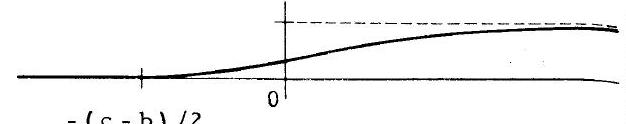
\includegraphics[max width=\textwidth]{2022_07_16_f4e476ee2159dc67e746g-47}

\begin{enumerate}
  \setcounter{enumi}{2}
  \item 
\end{enumerate}
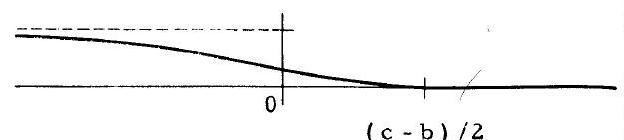
\includegraphics[max width=\textwidth]{2022_07_16_f4e476ee2159dc67e746g-47(1)}

\begin{enumerate}
  \setcounter{enumi}{3}
  \item 
\end{enumerate}
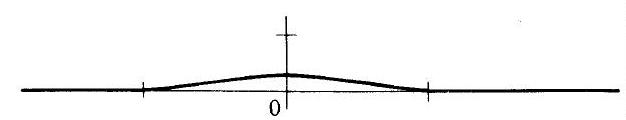
\includegraphics[max width=\textwidth]{2022_07_16_f4e476ee2159dc67e746g-47(2)}

\begin{enumerate}
  \setcounter{enumi}{4}
  \item 
\end{enumerate}
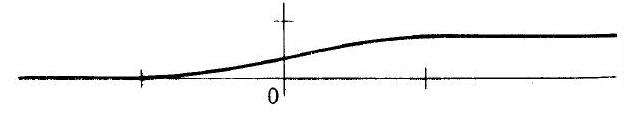
\includegraphics[max width=\textwidth]{2022_07_16_f4e476ee2159dc67e746g-47(3)}

\begin{enumerate}
  \setcounter{enumi}{5}
  \item 
\end{enumerate}
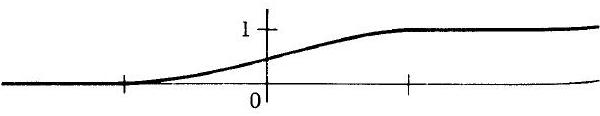
\includegraphics[max width=\textwidth]{2022_07_16_f4e476ee2159dc67e746g-47(4)}

iraph of $\mathrm{f}$ :

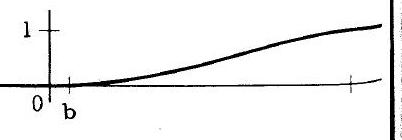
\includegraphics[max width=\textwidth]{2022_07_16_f4e476ee2159dc67e746g-47(5)}

Chap. 6 Riemannian Manifolds and Submanifolds

(a) $M$ is paracompact,

(b) Madmits a Riemannian metric,

(c) $M$ is second-countable (completely separable).

Proof. We show (a) implies (b) and give references for the other implications whose proofs are purely topological.

Assuming (a), apply lemma 4 to obtain a locally finite cover $\left[U_{\alpha}\right]$ with the partition of unity $\left[g_{\alpha}\right]$. On each coordinate neighborhood $U_{\alpha}$, define a local Riemannian metric tensor $<,>_{\alpha}$ by demanding the coordinate map be an isometry. Then the tensor $g_{\alpha}<,>_{\alpha}$ is a global $C^{\infty}$ tensor on $M$ that vanishes outside $U_{a^{*}}$ At any point $m$ in $M$, for $X$ and $Y$ in $M_{m}$, let $\left\langle X, Y>=\Sigma_{\alpha} \hat{s}_{\alpha}(m)\langle X, Y\rangle_{\alpha}\right.$. This defines a $C^{\infty}$ Riemannian metric tensor on $M$ which shows (a) implies (b).

Assuming (b), then from section $2.6$ we know $M$ is a metric space and hence must be paracompact (see Kelley, p. 160). "Thus (b) implies (a). That (c) implies (a) follows from Hocking and Young, p. 79. To show (b) implies (c), we refer the reader to Chapter 6 in Kelley. The metric can be used to define a uniform structure on $M$ which must admit a countable base (see Kelley, p. 186).// For theorems concerning the imbedding of manifolds in other manifolds see Sternberg, Auslander and Mackenzie, or Smale ${ }^{2}$.

Problems. All manifolds will be Riemannian unless otherwise stated.

\begin{enumerate}
  \setcounter{enumi}{49}
  \item If $M$ is semi-Riemannian and $D$ satisfies (4), then $D$ is metric preserving. Show that $D$ is metric preserving iff for parallel fields $Y$ and $Z$ along a curve o for function $\langle\boldsymbol{Y}, Z\rangle$ is constant On $\sigma_{0}$

  \item Let $R$ and $R^{\prime}$ be two linear map valued skew-symmetric 2covariant tensors whose corresponding $K$ and $K^{\prime}$ satisfy properties (a) thru (d) on p. 124. Show $K=K^{\prime}$ iff $R=R^{\prime}$.

  \item If $f$ is a $C^{\infty}$ strictly conformal map, show $f_{*}$ has no kernel and preserves angles. If $f$ is a complex analytic map, show $\left\langle f_{*} X_{p}, f_{*} Y_{p}>=\left|f^{\prime}(p)\right|^{2}<X_{p}, X_{p}>\right.$, where $f: C \rightarrow C$.

  \item Let $f: M \rightarrow M^{\prime}$ be a strictly conformal map with scale function $F$. Show $f$ is (Riemannian) connexion preserving iff $F$ is

\end{enumerate}
Fio. 6.1 Constructino a $c^{\infty}$ Sten Function constant and $f(M)$ is flat. If $f$ is an isometry, show $f$ preserves the curvature tensor and the Riemannian curvature.

\begin{enumerate}
  \setcounter{enumi}{53}
  \item With the standard hypothesis of section 3.3, show if $f$ is connexion preserving, then $M$ is a sphere, a plane, or a right circular cylinder (see Hicks ${ }^{2}$ ).

  \item Let $M$ be a hypersurface in $R^{n}$, let $N$ be a $C^{\infty}$ unit normal, let $g$ be in $C^{\infty}(M, R)$, and let $f_{t}: M \rightarrow R^{n}$ by $f_{t}(p)=p+t g(p) N$ Show that $\left(f_{t}\right)_{*} X=X+t(X g) N+\operatorname{tg} L(X)$ for $X$ tangent to $M$. If ${ }^{p}$ $f_{t}$ is an isometry for $t>0$, show that $M$ is flat.

  \item Generalize the first two theorems in section $6.5$ to the case of a $k-s u b m a n i f o l d$ that is framed in an $n$-manifold for $1<k<n$ (see Hicks ${ }^{1}$ ). In the second theorem, if $k=2$ and $n=3$, show $\bar{K}(P)=K(P)$ iff $g$ is a line of curvature on $M$.

  \item If $u$ and $v$ are orthonormal coordinates with $\operatorname{domain} A$ on a 2 manifold (thus $\partial / \partial u$ and $\partial / \partial v$ are orthonormal), show the coordinate curves are geodesics and $K \equiv 0$ on $A$.

  \item (K. Leisenring) Show that $f(u, v)=(\cos u \cos v, \cos u \sin v$, $\sin u \cos v, \sin u \sin v)$ is an isometric imbedding of the flat torus $T$ into the unit sphere $S^{3}$ in $R^{4}$. Show the total (imbedded) curvature of $f(T)$ in $S^{3}$ is a constant negative one.

  \item Let $M$ be connected with symmetric connexion $D$ and let $L_{p}$ : $M_{p} \rightarrow M_{p}$ be a $C^{\infty}$ linear map valued function on $M .$ If Tor ${ }_{p} \equiv 0$ and all points are $L$-umbilic, show $L$ is a constant multiple of the identity map.

  \item Show that every isometry of $R^{n}$ can be factored uniquely into an orthogonal map followed by a translation. If $f_{i}: R^{n} \rightarrow R^{n}$ is orthogonal, show $f_{*}=f$ in a natural way.

  \item If $e_{1}, \ldots, e_{n}$ is an orthonormal base field with dual base $w_{1}$, $\ldots, W_{n}$ and $M$ has constant Riemannian curvature $K$ show the associated curvature forms $R_{i j}=K W_{i} \wedge w_{j}$

  \item If $M$ has constant Riemannian curvature $K$ and one defines a metric on $M \times M$ by $\left\langle\left(X_{1} ; Y_{1}\right),\left(X_{2} ; Y_{2}\right)\right\rangle=\left\langle X_{1}, X_{2}\right\rangle+\left\langle V_{1}\right.$ $\boldsymbol{Y}_{2}>$, does $M \times M$ have constant curvature? 62. If $x_{1}, \ldots, x_{n}$ are coordinates on a hypersurface $U$ in $R^{n+1}$, let $x_{i}=\partial / \partial x_{i}, g_{i j}=\left\langle X_{i}, X_{j}>b_{i j}=\left\langle L X_{i}, X_{j}\right\rangle\right.$, and $L X_{i}=\Sigma_{i} a_{i j} X_{i}$. Show that $a_{i j}=\Sigma_{r}\left(g^{-1}\right)_{i r} b_{r j}$ (Weingarten equation), $R_{j k h}^{i}=$ $\Sigma_{r}\left(g^{-1}\right)_{i r}\left(b_{h j} b_{r k}-b_{k j} b_{r h}\right)$ (Gauss-curvature equation), and

\end{enumerate}
$$
\frac{\partial b_{i r}}{\partial x_{s}}-\frac{\partial b_{i s}}{\partial x_{r}}=\Sigma_{r}\left(b_{k r} \Gamma_{i s}^{k}-b_{k s} \Gamma_{i r}^{k}\right)
$$
(Codazzi-Maniardi equation).

\begin{enumerate}
  \setcounter{enumi}{63}
  \item If $M$ is a Hausdorff $C^{\infty}$ manifold, $A$ is a compact subset of $M, B$ is open in $M$, and $A \subset B$, show there is an $f$ in $C^{\infty}(M, R)$ with $f(A)=0, f(M-B)=1$, and $0 \leq f(M) \leq 1$.
\end{enumerate}
\section{Operators on Forms and Integration}
This chapter develops more structure on a manifold. To conserve space, the treatment is fairly blunt and many computational details are omitted. In the first four sections $M$ is a $C^{\infty} n$-manifold and $A$ is an open set in $M$.

Section 7.1. Exterior derivative.

For $p \geq 0$ we define the exterior differentiation map $d: F p(A) \rightarrow$ $F^{p+1}(A)$ where $F p(A)$ is the set of $C^{\infty} p$-forms on $A$. If $f$ in $F^{0}(A)$ and $X$ is a $C^{\infty}$ field on $A_{\text {p }}$ then $d f(X)=X f$. For $p>1$, letting $w$ be a $(p-1)$ form on $A$ and $X_{1 p . .,} X_{p}$ be $C^{\infty}$ fields on $A$, then
$$
\begin{gathered}
d w\left(X_{1}, \ldots, X_{p}\right)=\Sigma_{j=1}^{p}(-1)^{j+1} X_{j} W\left(X_{1}, \ldots, \hat{X}_{j}, \ldots, X_{p}\right)+ \\
\Sigma_{i<j}(-1)^{i+j} w\left(\left[X_{i}, X_{j}\right], X_{1}, \ldots, \hat{X}_{i}, \ldots, \hat{\hat{X}}_{j}, \ldots, X_{p}\right),
\end{gathered}
$$
where $\hat{X}$ indicates that the field $X$ is omitted as an argument.

Notice that the definition is consistent with the partial definition in section 5.2. One proves that $d w$ is in $F^{p}(A)$ by using the characterization theorem in Chapter 4. We outline the argument. That $d w$ is linear with respect to addition is trivial. That $d w$ is alternating can be shown by switching two arguments and examining the terms that don't immediately change signs (this must be done carefully). That $d w$ is linear over the ring $F^{0}(A)$ then need only be checked in one slot.

Proposition. The operator $d$ has the following properties:

(1) $d(w+v)=d w+d v$, where $w$ and $v$ are in $\mathrm{F}^{p}(A)$.

(2) $d(w \wedge v)=((d w) \wedge v)+(-1)^{p}(w \wedge d v)$, for $W$ in $F^{p}(A)$ and $v$ any form on $A$. (Any operator with this property is called an anti. derivation.)

(3) $d^{2}=d \circ d=0$.

Proof. Property (1) follows trivially from the definitions of $d$ and addition of functionals. For the other two properties we first obtain a local representation of $d .$ Let $x_{1}, \ldots, x_{n}$ be a coordinate system on an open set $U$, and let $X_{i}=\partial / \partial \mathrm{x}_{i^{*}}$ Then on $U$, a $(p-1)$-form $w$ may by represented by $w=\sum a_{i_{1} \ldots i_{p-1}} d x_{i_{1}} \wedge_{\ldots} \ldots d x_{i}$, where the sum is over all indices such that $1 \leq i_{j} \leq n$ and $i_{1}<i_{2}^{p-1}<_{0}<i_{p-1}$, and $a_{i}$ $i_{p-1}=w\left(X_{i_{1}}, \ldots, X_{i_{p-1}}\right) . d w=\sum d a_{i_{1}} \ldots i_{p-1} \wedge d x_{i_{1}} \wedge_{\ldots}, \wedge d W_{i_{p-1}}$, which is proved by applying both sides to $\left(X_{k}, \ldots, X_{k}\right)$ for $k_{1}<k_{2} \ldots<k_{p}$ $\operatorname{Since}\left[X_{r}, X_{s}\right]=0, d w\left(X_{k}, \ldots, X_{k_{p}}\right)=\sum_{i=1}^{p}(-1)^{f^{p}+1} X_{k_{j}} a_{k_{1} \ldots k_{j} \ldots k_{p}}$, while $\left[\sum d a_{i_{1}} \ldots i_{p-1} \wedge d x_{i_{1}} \wedge \ldots \wedge d x_{i}{ }_{p-1}\right]\left(X_{k_{1}}, \ldots, X_{k}\right)=d a_{k}{ }_{2} \ldots k_{p}\left(X_{k}\right)-$ $d a_{k_{1} \hat{k}_{2} \ldots k_{p}}\left(X_{k_{2}}\right)+\ldots=d w\left(X_{k_{1}}, \ldots, X_{k}\right)$

To prove property (2), first let $f$ and $g$ be functions in $F^{0}(A)$ and note $d(f g)=(d f) g+f(d g)$ follows from the derivation property of vectors. Next observe that because of (1) and the local representation above, one need only verify (2) for forms of the type $w=f d x_{1} \wedge \ldots, \wedge$ $d x_{p}$ and $v=g d y_{1} \wedge \ldots \wedge d y_{t}$, where $x_{i}$ and $y_{i}$ are functions chosen from the members of a coordinate system. Then $W \wedge V=f g d x_{1} \wedge \ldots$ $d x_{p} \wedge d y_{1} \wedge \ldots \wedge d y_{r}$, and $d(w \wedge v)=d(f g) \wedge d x_{1} \wedge_{\ldots} . . \wedge d y_{t}=(g d f+f d g) \wedge$ $d x_{1} \wedge \ldots \wedge d y_{r}=d w \wedge v+(-1)^{p_{W}} \wedge d v$.

For property (3) we first show $d^{2} f=0$ for a $C^{\infty}$ function $f$ in $F(A)$. Locally, $d f=\sum_{i=1}^{n}\left(\partial f / \partial x_{j}\right) d x$, so $d^{2} f=\sum^{n},\left(\partial^{2} f / \partial x_{i} \partial x_{j}\right) d x_{i} \wedge d x_{j}=$

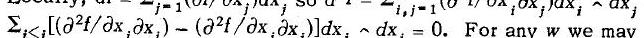
\includegraphics[max width=\textwidth]{2022_07_16_f4e476ee2159dc67e746g-49}\\
represent dw locally as a sum of products of $d f^{\prime}$ s for functions $f$; hence by (2) each term in $d^{2} w$ has a factor $d^{2} f=0$, so $d^{2} W=0 . / /$

Letting $F(M)=\sum_{k=0}^{n} F^{k}(M)$ be the direct sum of the modules of forms of homogenevus type, endowed with its exterior multiplication

\section{Chap. 7 Operators on Forms and Integration}
structure and exterior derivative operator $d$, one obtains a graded differential algebra which is called the Cartan differential algebra of $M$. If $f: M \rightarrow N$ is $C^{\infty}$, then $d \circ f^{*}=f^{*} \circ d$ on $F(N)$, and it is sufficient to check this only on 0 -forms and 1 -forms.

There are other ways to define $d$, indeed one natural way is to define $d$ via a local representation, get the desired properties, and then show it is independent of the local representation (see Chevalley ${ }^{1}$, p. 146). Then the invariant formula we took as definition must be verified. Our treatment in this and the following sections is similar to that of Palais ${ }^{1}$

\section{Section 7.2. Contraction.}
Let $X$ be a $C^{\infty}$ vector field on the open set $A .$ An operator $C_{X}$, called contraction by $X$, which maps $F p(A)$ into $F p-1(A)$ is defined as follows: (a) if $f$ in $F^{0}(A)$, let $C_{X} f=0$, and (b) if $w$ in $F p(A)$ for $p>0$, let $\left(C_{X} w\right)\left(X_{1}, \ldots, X_{p-1}\right)=w\left(X_{1}, X_{1}, \ldots, X_{p-1}\right)$

Proposition. The operator $C$ has the following properties:

(1) $\left(C_{X}\right)^{2}=0$

(2) $C_{x}(w+v)=C_{x} w+C_{x}$

(3) $C_{X+Y}=C_{X}+C_{Y}$

(4) $C_{f X}=f C_{X}$,

(5) $C_{X}(w \wedge z)=\left(C_{X} w\right) \wedge z+(-1)^{P}\left(w \wedge C_{X} z\right)$,

for $f$ in $F^{0}(A), X$ and $Y$ in $T^{1,0}(A), W$ and $v$ in $F p(A)$, and $z$ in $F q(A)$.

Proof. Properties (1) through (4) are trivial. Property (5) follows by induction on $p$, and it is sufficient to prove it when $w$ is a product of $p$ 1-forms by the local representation of forms.//

The operator $C_{X}$ can be defined on covariant tensors and mixed tensors in an obvious way (with only (2), (3), and (4) valid in general), and one can let $C_{X}$ be zero on pure contravariant tensors. Properties (3) and (4) indicate $C$ is a tensor map (an anti-derivation valued Iform of degree $-1$ on $F(A))$, There is another form of "contraction" induced by the natural identification of tensors of type 1,1 and linear maps. Let $W$ be an $n$-dim vector space over $R$. For $r>0, s>0,1 \leq i \leq r, 1 \leq j \leq s$ define $t r^{i, j}$ : $T^{r}, s(W) \rightarrow T^{t-1}, s-1(W)$ by taking $\theta$ in $T^{r}, s(W), W_{1}, \ldots, W_{r-1}$ in $W^{*}$, and $X_{1, \ldots, X_{s-1}}$ in $W$ and letting

(2) $\left(t^{i, i \theta)}\left(w_{1}, \ldots, w_{r-1}, X_{1}, \ldots, X_{s-1}\right)=\right.$
$$
\sum_{k=1}^{n} \theta\left(w_{1}, \ldots, w_{i-1}, Z_{k}, w_{i}, \ldots, w_{t-1}, X_{1}, \ldots, X_{j-1}, Z_{k}, X_{j}, \ldots, X\right.
$$
where $Z_{1}, \ldots, Z_{n}$ is a base of $W$ and $z_{1}, \ldots, z_{n}$ the dual base of $W^{*}$. One checks easily that $t^{i}, i \theta$ is well-defined independently of the particular base used. If $\theta$ in $T^{1,1}(W)$, let $t^{1}, 1 \theta=t r \theta$. The above operator induces an operator $t r^{i, j}: T^{r}, s(A) \rightarrow T^{r-1}, s-1(A)$ for an open set $A$ in

\section{Section 7.3. Lie derivative.}
Let $X$ be a $C^{\infty}$ vector field on the open set $A .$ An operator $L_{X}$, called the Lie derivative via $X$, which maps $T^{r}, s(A)$ into itself, is defined as follows: (a) if $f$ in $F^{0}(A), L_{X} f=X f ;$ (b) if $Y$ in $T^{1,0}(A)$, $L_{X} Y=[X, Y] ;(\mathrm{c})$ if $W$ in $T^{0,1}(A),\left(L_{X} W\right)(Y)=X W(Y)-W([X, Y]) ;$ and (d) if $\theta$ in $T^{r}, s(A), w_{1}, \ldots, w_{t}$ in $T^{0,1}(A)$, and $Y_{1}, \ldots, Y_{s}$ in $T{ }^{1,0}(A)$, then $L_{x} \theta$ is defined by solving for it in the equation

(3)
$$
\begin{aligned}
&L_{X}\left[\theta\left(w_{1}, \ldots, w_{r}, Y_{1}, \ldots, Y_{s}\right)\right]=\left(L_{X} \theta\right)\left(w_{1}, \ldots, Y_{s}\right) \\
&\quad+\theta\left(L_{X_{1}}, w_{2}, \ldots, Y_{s}\right)+\ldots+\theta\left(w_{1}, \ldots, Y_{s-1}, L_{X} Y_{s}\right)
\end{aligned}
$$
We call $L_{x}$ a complete derivation because of the property $(d)_{\text {, }}$ and note all terms in (3) are well-defined by (a), (b), and (c) except the $L_{X} \theta$ term (indeed, (c) is "defined" by (d)). One shows $L_{X} \theta$ is a tensor by checking the linearity over $F^{0}(A)$.

Proposition. The operator $L_{x}$ has the following properties:

(1) $L_{X}$ preserves forms,

(2) $L_{x}(w+z)=L_{x} w+L_{x} z$ (3) $L_{x}(w \otimes v)=\left(L_{X} w\right) \otimes v+w \otimes L_{x} v$

(4) $L_{x}(\alpha \wedge \beta)=\left(L_{x} \alpha\right) \wedge \beta+a \wedge L_{x} \beta$

where $w$ and $z$ are tensors of the same type, $v$ is any tensor, and $a$ and $\beta$ are forms.

Proof. An exercise (for (4) use $\left.L_{X}\left[(\alpha \otimes \beta)^{\pi}\right]=\left[L_{X}(\alpha \otimes \beta)\right]^{\pi}\right)$.

There is a more geometric definition of the Lie derivative $L_{X}$ on covariant tensors which we now discuss. Suppose the vector field $X$ is defined and $C^{\infty}$ on all of $M$. For each $m$ in $M$ let $f_{m}(t)$ be the integral curve of $X$ (section 1.5) through $m$ with $f_{m}(0)=m$. we know $f_{m}$ defined for $t$ in a neighborhood of zero, but suppose each $f_{m}$ is defined for all $t$ and $R$. Then for each $t$ in $R$ we could define a map $F_{t}: M \rightarrow M$ by $F_{t}(m)=f_{m}(t)$, with the properties $F_{t} \circ F_{s}=F_{t+s}$ and $F: M \times R \rightarrow M$ by $F(m, t)=F_{t}(m)$ would be $C^{\infty}$ (from the fact that $X$ was $C^{\infty}$ and the $C^{\infty}$ dependence of solutions of ordinary differential equations upon initial conditions). Each $F$, would be a diffeo, since $\left(F_{t}\right)^{-1}=F_{-t}$ and $F_{0}$ is the identity map. A map $F$ with the above properties is called a 1-parameter group of differentiable transforma tions of $M$, and $X$ is called its infinitesimal generator.

In general $f_{m}$ is not defined for all $t$, but one does obtain a local 1-parameter group of local transformations in a neighborhood of each $m$ in $M$; i.e., for each $m$ in $M$ there is a neighborhood $U$ of $m$, a real number $b>0$, and a map $F: U \times(-b, b) \rightarrow M$ such that (1) $F$ is $C^{\infty}$, (2) for $t$ in $(-b, b), F_{t}: U \rightarrow F_{t}(U)$ is a diffeo, (3) for $t, s$, and $t+s$ in $(-b, b), F_{t} \circ F_{s}=F_{t+s}$, and (4) for fixed $p$ in $U_{,} f_{p}(t)=F_{t}(p)$ is an integral curve of $X$. For more details see Palais 1 and 2 and Nomizu 1 (p. 5).

LEMMA 1. Let $Y$ be a $C^{\infty}$ field in a neighborhood of $m$ in $M$. $W e$ choose $U$ and $b$ in the preceding paragraph to be sufficiently small so the image of $F$ is contained in the domain of $Y$. Then
$$
[X, Y]_{m}=\lim _{t \rightarrow 0}\left[\left(F_{-t}\right)_{*} Y_{F(m, t)}-Y_{m}\right] / t .
$$
Proof. See Nomizu 1 (p, 8).

\section{Notes on Differential Geometry}
Assuming lemma 1, which gives us another geometric interpretation of the bracket, it is trivial to show the following lemma.

LEMMA 2. Let $w$ be a $C^{\infty} p$-form at $m .$ Then
$$
\left(L_{X} w\right)_{m}=\lim _{t \rightarrow 0}\left[\left(F_{t}^{*} w\right)_{m}-w_{m}\right] / t
$$
where
$$
\left(F_{t}^{*} W\right)_{m}\left(Y_{1}, \ldots, Y_{p}\right)=W_{F(m, t)}\left(\left(F_{t}\right)_{*} Y_{1}, \ldots,\left(F_{t}\right)_{*} Y_{p}\right)
$$
The following is a useful relation between $d, L_{X}$, and $C_{X}$

Proposition. If $X$ is a $C^{\infty}$ field on $A$, then $L_{X}=d \circ C_{X}+C_{X} \circ d$ when applied to $C^{\infty}$ forms on $A$.

Proof. We verify this equality on function (0-forms) and 1-forms. This is sufficient to prove the proposition, since locally a form is a sum of products of functions and 1-forms, and the operators which we equate above are both derivations; hence their value on any form is determined by the values on functions and 1-forms.

For $f$ in $F^{0}(A), d C_{X}(f)+C_{X} d(f)=0+d f(X)=X f=L_{X} f .$ For $W$ in $F^{1}(A),\left(d C_{X}+C_{X} d w\right)(Y)=Y W(X)+d w(X, Y)=Y w(X)+X W(Y)-$ $Y w(X)-w([X, Y])=\left(L_{X} w\right)(Y) . / /$

Section 7.4. General covariant derivative.

Let $D$ be a connexion on $M$, and let $X$ be a $C^{\infty}$ field on the open set $A$. An operator $D_{X}$, called the covariant derivative via $X$, which maps $T^{r}, s(A)$ into itself, is defined by using the recipe for defining $L_{X}$. The definition of $D_{X}$ proceeds exactly as the definition for $L_{x}$ except for (b), and if $Y$ in $T^{1,0}(A), D_{X} Y$ is given by the connexion $D$ (see section $5.1$ ).

When $D_{X}$ is substituted for $L_{X}$ in the first proposition of the previous section, one obtains valid properties for $D_{X}$.

An operator $\Delta$, called the general covariant derivative operator, which maps $T^{r, s}(A)$ into $T^{r, s+1}(A)$ is induced by $D$. If $\theta$ is in $T^{r}, s(A)$, $w_{1}, \ldots, w_{r}$ are in $T^{0,1}(A)$, and $Y_{1}, \ldots, Y_{s+1}$ are in $T^{1}, 0(A)$, then

\section{Chap. 7 Operators on Forms and Integration}
$(4)(\Delta \theta)\left(w_{1}, \ldots, w_{P}, Y_{1}, \ldots, Y_{s-1}\right)=\left(D_{Y}, \theta\right)\left(w_{1}, \ldots, w_{s}, Y_{19 \ldots,} Y_{s}\right)$

That $(\Delta \theta)$ is a tensor is left as a problem. If $\theta$ and $\phi$ are tensors of the same type, then $\Delta(\theta+\phi)=\Delta \theta+\Delta \phi$, but $\Delta$ is not a tensor (see problem 64).

If $1 \leq i \leq p$ and $1 \leq j \leq q$, then

(5) $\Delta \circ t r^{i, j}=t r^{i, j} \circ \Delta$

on $T^{p, q}(A)$

An operator div, called the divergence, which maps $T^{t, s}(A)$ into $T^{r-1}, s(A)$, for $r>0$ and $s \geq 0$, is defined by div $=t r^{r}, s+1 \circ \Delta$. We write div $\theta=\operatorname{tr}(\Delta \theta)$, where we assume the trace is taken on the last covariant slot and the last contravariant slot. A tensor $\theta$ is conservative if div $\theta=0$

The Riemann-Christoffel curvature tensor of type 1,3 is the tensor $K$ in $T^{1,3}(A)$ defined by

(6) $K(w, X, Y, Z)=w(R(Y, Z) X)$

for $w$ in $T^{0,1}(A)$ and $X, Y$, and $Z$ in $T^{1,0}(A)$. The second Bianchi identity is the equation

(7) $(\Delta K)(w, X, Y, Z, W)+(\Delta K)(w, X, W, Y, Z,)+(\Delta K)(w, X,$,$Z ,$ $W, Y,)=$,

which is valid if $D$ is symmetric, and it is proved by noting the expression

(8) $D_{W}(R(Y, Z) X)-R(Z,[Y, W]) X-R(Y, Z)\left(D_{W} X\right)$

when written on three lines, permuting $W, Y, Z$ cyclically from line to line, and then adding the three lines, yields zero.

The Ricci tensor is the 2-covariant tensor

(9) $\operatorname{Ric}(X, Y)=\left(t r^{1,2} K\right)(X, Y)=-\left(\operatorname{tr}^{1},{ }^{3} K\right)(X, Y)$ (and this is the negative of the "classical" Ricci tensor). Notice $\left(t r^{1}, K\right)(X, Y)=\operatorname{tr} R(X, Y)$, The Ricci curvature of a vector $X$ is the number $\operatorname{Ric}(X, X)$ (and this agrees with the "classical" Ricci curvature). If $D$ is symmetric, the first Bianchi identity implies

(10) $\operatorname{Ric}(X, Y)=\operatorname{Ric}(Y, X)+\operatorname{tr} R(X, Y)$

If $D$ is Riemannian, then $R(X, Y)$ is skew-symmetric by (c) in section 6.2, so Ric is symmetric. Hence there exists a self-adjoint linear map $R^{*}$, called the Ricci map, defined on each $M_{\mathrm{m}}$ with $\operatorname{Ric}(X, Y)=\langle R *(X), Y>;$ indeed
$$
R^{*}(X)=\sum_{j=1}^{n} R\left(X, Z_{j}\right) Z_{j}
$$
for an orthonormal base $Z_{1}, \ldots, Z_{n^{*}}$ By $(11), R^{*}$ is $C^{\infty}$. The scalar curvature $S(m)$ at each $m$ in $M$ is defined by $S(m)=t r\left(R^{*}\right)_{m}$.

A (semi-) Riemannian metric induces many operations called "raising" and "lowering" of indices which we now explain. The non-singular metric tensor induces a non-singular linear map $G$ of $M_{m}$ onto $M_{m}^{*}$ for each $m$, i.e., if $X$ in $M_{m}$, then $G(X)(Y)=\left\langle X, Y>\right.$. We let $G_{*}$ denote the inverse map of $M_{m}^{*}$ onto $M_{m}$. If $w$ in $M_{m}^{*}$, then $\left\langle G_{*} W_{0} X\right\rangle=W(X)$. If $1 \leq i \leq r, 1 \leq j \leq s+1$, and $\theta$ is in $T^{r}, s$ define $G^{i, j} \theta$ in $T^{r-1, s+1}$ by
$$
\left(G^{i, j} \theta\right)\left(w_{1}, \ldots, W_{r-1}, X_{1}, \ldots, X_{s+1}\right)
$$
$$
\begin{aligned}
& =\theta\left(w_{1}, \ldots, w_{i-1}, G\left(X_{j}\right), w_{i}, \ldots, w_{t-1}, X_{1}, \ldots, \widehat{X}_{j}, \ldots, X_{s+1}\right)
\end{aligned}
$$
Similarly, define $G_{*}^{i, j}: T T^{r}, s \rightarrow T^{r}+1, s-1$ for $1 \leq i \leq r+1$ and $1 \leq j \leq s$ by taking the form in the $i$ th covariant slot (of the new tensor), applying $G_{*}$, and inserting it into the $j^{t h}$ contravariant slot (of the old tensor), Thus $G^{1,1}=G$ on $T^{1}, 0$, and the 1,1 -tensor $\bar{R}$ associated with $R^{*}$ is given by $R=G_{*}{ }^{1}, 1$ Ric (where $\bar{R}(w, X)=w(R * X)$ ). If $f$ is in $C^{\infty}(M, R)$, the gradient field of $f$ is the field grad $f=G_{*}(d f)$ and the Laplacian of $f$ is the function del $f=\operatorname{div}(\operatorname{grad} f)$; (sometimes the notation del $f=$ $\Delta f$ is used).

The operators $G^{i_{1} j}$ and $G_{*}^{i_{0} j}$ commute with $\Delta$ when possible, i.e., $\Delta \circ G^{i, j}=G^{i, j} \circ \Delta$ on $T^{r}, s$ if $j \leq s+1$ and
$$
\Delta \circ G_{*}^{i, j}=G_{*}^{i, j} \circ \Delta \text { on } T^{r, s} \text { if } i \leq t+1 .
$$
As an example of the use of these oper ations we prove that

(15) $\Delta S=2 \operatorname{div} \bar{R}$

which is used in general relativity. Let $Z_{1}, \ldots, Z_{n}$ be an orthonormal base of $M_{m}$ and $W_{1}, \ldots, W_{n}$ the dual base. The second Bianchi identity implies

$\left.\left.\Sigma_{i, j}\left[\Delta K_{j}, Z_{i}, Z_{j}, Z_{i}, X\right)+\Delta W_{i}, Z_{i}, X, Z_{j}, Z_{i}\right)+K\left(w_{j}, Z_{i}, Z_{i}, X, Z_{j}\right)\right]=$ The first term of the sum gives $(\Delta S)(X)$, while the other two each give $-(\operatorname{div} R)(X)$. For
$$
\begin{aligned}
(\Delta S)(X) &=\left(\Delta t r^{1,1} G_{*}{ }^{1,1} t r^{1,2} K\right)(X) \\
&=\left(t r^{1},{ }^{1} G_{*}{ }^{1,1} t^{1}{ }^{1,2} \Delta K\right)(X) \\
&=\sum_{i j} \Delta K^{K}\left(w_{j}, Z_{i}, Z_{j}, Z_{i}, X\right)
\end{aligned}
$$
$(\operatorname{div} \bar{R})(X)=\left(t r^{1,2} \Delta G_{*}{ }^{1,1} t_{t r}, 2, K\right)(X)$
$$
=-\Sigma_{i, j} \Delta K\left(w_{j}, Z_{i}, X, Z_{j}, Z_{i}\right), \text { and }
$$
$(\Delta K)\left(w_{j}, Z_{i}, Z_{i}, X, Z_{j}\right)=\left(\Delta G^{1}, K\right)\left(Z_{j}, Z_{i}, Z_{i}, X, Z_{j}\right)$
$$
\begin{aligned}
&=\left(\Delta G^{1}, 1 K\right)\left(Z_{i}, X, Z_{j}, Z_{i}, Z_{j}\right) \\
&=-\left(\Delta G^{1,1} K\right)\left(Z_{i}, Z_{i}, X, Z_{j}, Z_{j}\right)-\left(\Delta G^{1}, 1 K\right)\left(Z_{i}, Z_{j}, Z_{i}, X_{,} Z_{j}\right) \\
&=-(\operatorname{div} \bar{R})(X)
\end{aligned}
$$
by (c) and $\left(a^{\prime}\right)$ in section 6.2.

\section{Notes on Differential Geometry}
Section 7.5. Integration of forms and Stokes' theorem.

One integrates $p$-forms over $p$-chains, or singular $p$-chains, which we now define. Let $I^{p}=\left[a\right.$ in $\left.R^{p}: 0 \leq a_{i} \leq 1\right]$ denote the unit $p$-square for $p>0$, and $I^{\circ}=[0$ in $R] . \quad$ A $C^{\infty} p-c u b e ~ o$ on $M$ is an $M-$ valued $C^{\infty}$

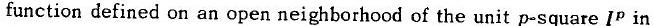
\includegraphics[max width=\textwidth]{2022_07_16_f4e476ee2159dc67e746g-53}\\
$R^{p}$. A real $C^{\infty} p$-chain $\mathrm{c}$ is a finite formal linear combination of $C^{\infty}$ $p$-cubes with real coefficients, thus $c=r_{1} \sigma_{1}+r_{2} \sigma_{2}+\ldots+r_{k} \sigma_{k}$ where $r_{j}$ in $R$ and $\sigma_{j}$ are $C^{\infty} p$-cubes. The set $C_{p}(M, R)$ of all real $C^{\infty} p-$ chains is an abelian group (actually an $R$-module) where one defines addition by adding the coefficients of corresponding $p$-cubes.

There are fancier ways of defining $C_{p}(M, R)$. Let $Q_{p}$ be the set of $C^{\infty} p$-cubes on $M$. Then $C_{p}(M, R)$ is isomorphic to set of all functions mapping $Q_{p}$ into $R$ which are zero except on a finite number of elements, and the addition and scalar multiplication structure on this function space is obvious. Similarly, one could define $C(M, Z)$, the set of integral $C^{\infty} p$-chains or $C^{\infty} p$-chains over the integers. Then $C_{p}(M, R)=R \quad{ }_{Z} C_{p}(M . Z)$. More generally one could define $C^{\infty} p^{-}$ chains over any ring $A$ with an identity element, and then by using the tensor product obtain the $A$-module of $C^{\infty} p$-chains on $M$ over any $A$-module. There are corresponding groups obtained from $C^{t} p-c h a i n s$ for any integer $r \geq 0$. These groups are fundamental objects of the cubical singular homology theory for $M$ and are studied in algebraic topology, (see Eilenberg and Steenrod). Because of our differential geometry bias, we restrict ourselves to real $C^{\infty}$ p-chains, and let $\mathrm{C}_{p}=\mathrm{C}_{p}(M, R)$

The support of a p-cube $\sigma$ is the set $|\sigma|=\sigma\left(I^{p}\right)$, the image of $I^{p}$

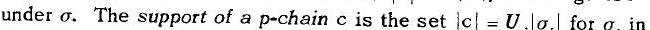
\includegraphics[max width=\textwidth]{2022_07_16_f4e476ee2159dc67e746g-53(1)}\\
$c$, where we say $\sigma_{i}$ in $c$ if the coefficient of $\sigma_{i}$ is non-zero, i.e., adopting the functional viewpoint $c\left(\sigma_{i}\right) \neq 0$ iff $\sigma_{i}$ in $c$.

To define the boundary map $\partial: C_{p} \rightarrow C_{p-1}$, define maps $\alpha_{i}^{1}$ and $a_{i}^{0}$ from $I^{p-1}$ into $I^{p}$ for $i=1, \ldots, p$ by
$$
a_{i}^{\varepsilon}\left(t_{1}, \ldots, t_{p-1}\right) \in\left(t_{1}, \ldots, t_{i-1}, \epsilon, t_{i}, \ldots, t_{p-1}\right)
$$
where $\epsilon=1$ or 0 . If $\sigma$ in $Q_{p}$, define $\partial \sigma=\sum_{1}^{p}(-1)^{i+1}\left(\sigma \circ a_{i}^{1}-\sigma \circ a_{i}^{0}\right)$, and call the $(n-1)$-cubes $\sigma \circ \alpha_{i}^{1}$ and $\sigma \circ \alpha_{i}^{0}$ faces of $\sigma .$ We extend $\partial$ to all of $C_{p}$ by demanding it be linear, i.e., $\partial\left(c_{1}+c_{2}\right)=\partial c_{1}+\partial c_{2}$ and $\partial(r \mathrm{c})=r \partial \mathrm{c}$ for $r$ in $R$. A straightforward computation shows $\partial^{2}=0$. For $p>0$, let $\sigma$ be a $C^{\infty} p$-cube, let $w$ be a $p$-form, and let $u_{1}, \ldots$, $u_{p}$ be the natural coordinate function on $R^{p}$. Since $\sigma^{*} w$ is a $p$-form on a neighborhood of $I^{p}$, we may define a $C^{\infty}$ function $f$ on $I^{p}$ by $\sigma^{*} W=f d u_{1} \wedge d u_{2} \wedge \ldots \wedge d u_{p}$. Then
$$
\int_{\sigma} W \equiv \int_{I} p^{*} W \equiv \int_{I} p
$$
where the integral on the right is the standard Riemann integral of $f$ over $I^{p}$ developed in advanced calculus. If $c=\sum_{1}^{k_{i}} \sigma_{i}$ is a $p$-chain, then $\int_{c} w=\sum_{1}^{k_{r_{i}}} \int_{\sigma_{i}} w$; thus for fixed $w$, the integral over $w$ is an $R$ -

homomorphism of $C_{p}$ into $R$. Since $\sigma^{*}$ is linear, it is trivial that $\int_{c}\left(w_{1}+w_{2}\right)=\int w_{1}+\int_{c} w_{2}$ for $p$-forms $W_{i}$ and a p-chain c.

For $p=0$, let $f$ be a function on $M$ and $\sigma_{m}$ the 0 -cube with $\sigma_{m}(0)=m$, then $\int_{\sigma} f=f(m)=\sigma_{m}^{*} f(0)$, and we extend the integral of $f$ over any

real 0-chain to be linear (as extended above).

Let $C^{p}=$ Hom $_{R}\left(C_{p}, R\right)$, which is the $R$-module of all $R$-linear homomorphisms of $C_{p}$ into $R$. The set $C^{p}$ is called the module of real $C^{\infty} p$-cochains of $M$. The adjoint $\delta$ of the boundary operator $\partial$ is called the coboundary operator and is defined by $\delta f(c)=f(\partial c)$ for $p$-cochain $f$ and a $(p+1)$-chain c. Thus $\delta: C^{p} \rightarrow C^{p+1}$ and $\delta^{2}=0$.

We define the Stokes'map $S: F p(M) \rightarrow C p$ which maps $p$-forms on $M$ into $C^{\infty} p$-cochains on $M$ by $[S(w)](c)=\int w$, for $c$ in $C_{p}$ The fol-

lowing theorem shows the Stokes' map commutes with the differential coboundary operator, i.e., $S \circ d=\delta \circ S$.

STOKES' THEOREM. Let $w$ be a $C^{\infty} p-$ form and $\sigma$ be a $C^{\infty}(p+$ 1)-cube, then

(18) $\int_{\sigma} d w=\int_{\partial \sigma} w$

Proof. Define $C^{\infty}$ functions $a_{1}, \ldots, a_{p+1}$ on $I^{p+1}$ by $\sigma^{*} W=\sum p^{+1} a_{i} d u_{1}{ }^{*}$ $d u_{2} \wedge \ldots \wedge \hat{d u}_{i} \wedge_{\ldots} \wedge d u_{p+1}$. Then

\section{Notes on Differential Geometry}
$$
\begin{aligned}
d\left(\sigma^{*} w\right) &=\sum_{i=1}^{p+1}\left(\sum_{i=1}^{p+1} \frac{\partial a_{i}}{\partial u_{j}} d u_{j}\right) \wedge d u_{1} \curvearrowright \ldots \wedge d u_{i} \cap \cdots \wedge d u_{p+1} \\
&=\left[\sum_{i=1}^{p+1}(-1)^{i+1} \frac{\partial a_{i}}{\partial u_{i}}\right] d u_{1} \wedge \cdots \wedge d u_{p+1} \cdot \\
c e \int_{\sigma} d w &=\int_{I^{p+1}} \sigma^{*} d w=\int_{I^{p+1}} d \sigma^{*} w=\int_{I^{p+1}}\left[\sum_{1}^{\left.p^{+1}(-1)\right)^{i+1}} \frac{\partial a_{i}}{\partial u_{i}}\right] \\
&=\sum_{1}^{p+1}(-1)^{i+1}\left[\int_{0}^{1} \int_{0}^{1} \cdots \int_{0}^{1} \frac{\partial a_{i}}{\partial u_{i}} d u_{1} d u_{2} \ldots d u_{p+1}\right] \\
&=\sum_{1}^{p+1}(-1)^{i+1} \int_{I^{p}}\left(a_{i} \circ \alpha_{i}^{1}-a_{i} \circ a_{i}^{0}\right)
\end{aligned}
$$
where we use Fubini's theorem and integrate first with respect to $i$ th coordinate to obtain the last equality.

For the other side we must compute $\int_{\sigma \circ \alpha_{i}^{\varepsilon}}=\int_{I^{p}}\left(\alpha_{i}^{\varepsilon}\right)^{*} \circ \sigma(w)$ for $\epsilon=0$ or 1. Notice $\left(\alpha_{i}^{\varepsilon}\right) * d u_{j}=d\left(\left(\alpha_{i}^{\varepsilon}\right)^{*} u_{j}\right)=d\left(u_{j} \circ a_{i}^{\varepsilon}\right)=d u_{j}, 0$, or $d u_{j \rightarrow 1}$ according as $j<i, j=i$, or $j>i$, respectively. Thus $\left(a_{i}^{\varepsilon}\right)^{*} \sigma^{*} W={ }^{*}$ $\left(a_{i} \circ \alpha_{i}^{\varepsilon}\right) d u_{1} \wedge_{\ldots} \wedge d u_{p}$ and
$$
\begin{aligned}
\int_{\partial \sigma} w &=\sum_{i=1}^{p+1}(-1)^{i+1}\left[\int_{\sigma \circ \alpha_{i}^{1}} w-\int_{\sigma \circ \alpha_{i}^{0}} w\right] \\
&=\sum_{i=1}^{p+1}(-1)^{i+1} \int_{I^{p}}\left(a_{i} \circ \alpha_{i}^{1}-a_{i} \circ a_{i}^{0}\right)
\end{aligned}
$$
which proves the desired equality.//

We remark that Stokes' theorem is simply a generalized "fundamental theorem of calculus." Let $f: M \rightarrow M^{\prime}$ be a $C^{\infty}$ map, let $w$ be a pform on $M^{\prime}$ and $\sigma$ a $p$-cube in $M$, then it is trivial to show $\int_{f o \sigma} w=$ $\int_{\sigma} f *$, which is essentially the classical substitution rule that deals with the behavior of integrals with respect to mappings.

The Stokes' map induces a map at the cohomology level that yields an algebra-isomorphism of the differential cohomology groups of a manifold with the real singular cohomology groups. This fact is called the de Rham theorem (see A. Weil, and problem 71).

\section{Chap. 7 Operators on Forms and Integration}
Section 7.6. Integration in a Riemannian manifold.

Let $M$ be a Riemannian manifold, let $\sigma$ be a $C^{\infty}$ curve in $M$, and let $f$ be a real valued $C^{\infty}$ function on the image of $\sigma$, i. e., let $f \circ \sigma$ be $C^{\infty}$. Consider a "piece" of $\sigma$, which we assume to be parameterized by arc length on the interval $[a, b]$, and define
$$
\int_{\sigma \mid[a, b]} f=\int_{a}^{b} f \circ \sigma(s) d s
$$
where $\sigma \mid[a, b]$ denotes the restriction of $\sigma$ to the interval $[a, b]$. Call the integral just defined the integral of $f$ over $\sigma$ restricted to $[a, b]$ and when the interval is understood, we write simply $\int f .$ If $f$ is a $C^{\infty}$ real valued function $f$ defined on a broken $C^{\infty}$ curve $\sigma$, we define $\int_{\sigma} f$ to be the sum of the integrals of $f$ over the finite number of $C^{\infty}$

sub-curves determining $\sigma$. Notice that by assuming $\sigma$ parametrized by arc length we are integrating over oriented or $d$ irected curves.

We wish to integrate real valued $C^{\infty}$ functions over other subsets of $M$, and in some cases over $M$ itself. This could be accomplished by using the Riemannian metric to define a measure on $M$, but for our purposes we need not be so general. First we define orientable manifolds and then utilize the theory developed above for integrate ing forms over chains.

An $n$-dimensional manifold $M$ is orientable if there is a non-vanish ing $C^{\infty} n$-form $w$ on $M$. When $M$ is orientable and we have selected $w$, we say $M$ is oriented (by $w$ ) and $w$ is an orientation of $M$. If $M$ is oriented by $w$, then an ordered base $e_{1}, \ldots, e_{n}$ of $M_{m}$ is positively oriented if $w_{m}=b w_{1} \wedge \ldots \wedge W_{n}$ where $b>0$ and $w_{i}$ are the l-forms dua to $e_{j} .$ We say $M$ is non-orientable when $M$ is not orientable. If $M$ is oriented and $e_{1}, \ldots, e_{n}$ a positively oriented base of $M$, then one verifies easily that a base $f \ldots, f$ of $M$ is positively oriented if and only if $\operatorname{det}\left(b_{i j}\right)>0$ where $f_{j}=\Sigma_{f} b_{i j} e_{i \cdot}$

For example, $R^{n}$ is orientable, and we orient it by choosing $W=d u_{1} \wedge \ldots \wedge d u_{n}$ where $u_{i}$ are the natural coordinate functions. It is is orientable. is orientable.

Let $M$ and $M^{\prime}$ be oriented n-manifolds. A non-singular $C^{\infty}$ map $f$ of $M$ into $M^{\prime}$ is orientation preserving if $f_{*}$ maps a positively oriented base onto a positively oriented base.

Let $M$ be an oriented Riemannian $n-\operatorname{manifold.~For} m$ in $M$ let $e_{1 g . . .}, e_{n}$ be a positively oriented orthonormal base of $M_{m}$ with dual base $w_{1} \ldots . . W_{n}$. Define the $n$-form $v$ by $v_{m}=W_{1} \wedge_{\ldots}, W_{n}$. The form $v$ is a well-defined (independent of the particular base) $C^{\infty} n$-form on $M$ called the volume element.

A major problem now confronts us: the problem of "triangulating" or "cubulating" a manifold. This is a theory for breaking the manifold into "nice pieces" over which one can integrate functions. For this purpose we define fundamental $n$-chains. Let $\operatorname{Int}(A)$ denote the interior of a set $A$.

Let $M$ be an oriented $C^{\infty} n$-manifold. A fundamental n-chain in $M$ is a chain $c=\sigma_{1}+\ldots+\sigma_{k}$ such that: (1) each $\sigma_{i}$ is an $n$-cube that is an orientation preserving diffeo onto its image; and (2) Int $\left(\left|\sigma_{i}\right|\right) \cap$ Int $\left(\left|\sigma_{j}\right|\right)$ is empty for $i \neq j .$ Figure $7.1$ gives a schematic diagram of a fundamental 2-chain (with the images of the faces of the canonical 2-cube numbered).\\

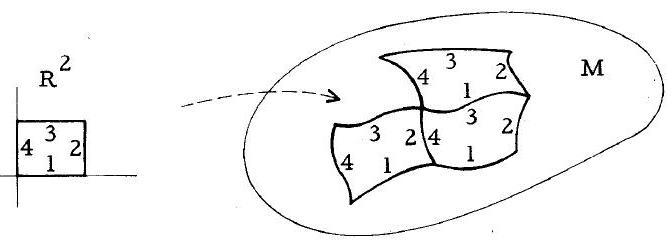
\includegraphics[max width=\textwidth]{2022_07_16_f4e476ee2159dc67e746g-55}

Fig. 7.1. A Fundamental 2-Chain

If $M$ is an oriented Riemannian $n$-manifold, $c$ is an $n$-chain, and $f$ is a $C^{\infty}$ real valued function whose domain contains $|c|$, then define

(20) $\int_{c} f=\int_{c} f v$

where $v$ is the volume element on $M$. Let a subset $A$ of $M$ be fundamental if there exists fundamental n-chain $c$ with $|c|=A$. Notice a fundamental set is compact. Proposition. If $c$ and $\tau$ are two fundamental $n$-chains with $|c|=$ $|\tau|=A$, and $f$ is a $C^{\infty}$ function whose domain contains $A$, then $\int f v=\int f v$. Thus define $\int f=\int f v$.

Proof. (King Lee). Let $c=\sigma_{1}+\ldots+\sigma_{t}$ and $\tau=\gamma_{1}+\ldots+\gamma_{s}$, and throughout this proof let $1 \leq i \leq r$ and $1 \leq j \leq$ s. If $A_{i j}=\left|\sigma_{i}\right| \cap\left|\gamma_{j}\right|$, let $B_{i j}=\left(\sigma_{i}\right)^{-1}\left(A_{i j}\right)$ and $C_{i j}=\left(\gamma_{j}\right)^{-1}\left(A_{i j}\right)^{\text {. Then } \gamma_{j}^{-1} \circ \sigma_{i}}$ is a diffeo of $B_{i j}$ onto $C_{i j}$ and

$\int_{B_{i j}}\left(\sigma_{i}\right) * * v=\int_{B_{i j}}\left(\sigma_{i}\right)^{*}\left(\gamma_{j} \circ \gamma_{j}^{-1}\right)^{* * V}=\int_{B_{i j}}\left(\gamma_{j}^{-1} \circ \sigma_{i}\right)^{*}\left(y_{j}\right)^{* f v}=\int_{C_{i j}}\left(y_{j}\right)^{* f V} .$

Hence, $\int_{c} f v=\Sigma_{i} \int_{\sigma_{i}} f v=\Sigma_{i, j} \int_{B}\left(\sigma_{i j}\right) * f v=\Sigma_{i, j} \int_{C_{i j}}\left(\gamma_{j}\right)^{*} f v=\int_{T} f v . / /$

If $M$ is a compact oriented n-manifold, then $M$ is a fundamental set (this is hard; see Cairns). Thus if $M$ is a compact oriented Riemanian manifold and $f$ is a $C^{\infty}$ real valued function on $M$, then $\int_{M} f$ is welldefined. To handle the non-compact case, define the suppor $t$ of a function $f$ to be the set $S_{f}$ that is the closure of the set $[p$ in $M$ :

$f(p) \neq 0]$. Since any compact set of $M$ is contained in a fundamental set (a non-trivial remark), if $M$ is oriented and Riemannian, $f$ is $C^{\infty}$ with compact support, and $S_{f} \subset$ fundamental set $A$, then $\int_{M} f=\int_{A} f$ is well-defined (independent of $A$ ).

The area, volume, or measure (depending on the appropriate dimension) of a fundamental set $A$ is the number $\int_{A} f$, where $f \equiv 1$ on $M$. For a deeper study of integration theory on manifolds see the book of Whitney ${ }^{2}$.

Problems. Let $M$ be a $C^{\infty} n-m a n i f o l d$ and 1 et $U$ be an open subset of $M$.

\begin{enumerate}
  \setcounter{enumi}{64}
  \item If $X$ and $Y$ are in $T^{1,},{ }^{\circ}(M), f$ and $g$ in $C^{\infty}(M, R)$, and $w$ in $T^{0,1}(M)$, show $L_{f X} w=w(X) d f+f\left(L_{X} w\right), L_{f X} Y=f\left(L_{X} Y\right)-d f(Y) X$ $L_{f X} g=f L_{X} g$, and $\Delta(f w)=f \Delta w+w \otimes d f$. Thus $L$ and $\Delta$ are not tensors.

  \item If $X$ is a $C^{\infty}$ vector field on $U, m$ in $U, Z_{1}, \ldots, Z_{n}$ a base of $M_{m}$ with dual base $w_{1}, \ldots, w_{n}$, show $(\operatorname{div} X)_{m}=\sum_{i=1}^{n} W_{i}\left(D_{i} X\right)$. Show that the divergence of a $C^{\infty}$ field on $R^{3}$ agrees with the advanced calculus definition.

  \item Let $A$ be in $T^{1,1}(U)$, let $Z_{1}, \ldots, Z_{k}$ be a $C^{\infty}$ base field on $U$, and let $w_{1}, \ldots, w_{k}$ be the dual base on $U$. Show $D_{X} w_{j}=$ $-\Sigma_{k} w_{j}\left(D_{X} Z_{k}\right) w_{k}$ and $\Sigma_{j}\left[A\left(D_{X} w_{j}, Z_{j}\right)+A\left(w_{j}, D_{X} Z_{j}\right)\right]=0$.

  \item Let $M$ be Riemannian, let $X_{1}, \ldots, X_{n-1}, T$ be an orthonormal base, and let $P_{i}$ be the plane section spanned by $X_{i}$ and $T$. Show Ric $(T, T)=\sum_{i=1}^{n-1} K\left(P_{i}\right)$.

  \item Prove formulas (5), (7), (13), and (14).

  \item If $D$ has zero torsion, show $d w(X, Y)=\left(D_{X} w\right)(Y)-\left(D_{Y} w\right)(X)$,

  \item If $M$ is Riemannian and $G(X, Y)=\langle X, Y\rangle$, show that a connexion $D$ is metric preserving iff $\Delta G=0$. Given arbitrary $A$ in $T^{0,3}(M)$ and $B$ in $T^{1,2}(M)$ with $A(X, Y, Z)=A(Y, X, Z)$ and $B(w, X, Y)=-B(w, Y, X)$ for all $w, X, Y, Z$, show there exists a unique connexion $D$ on $M$ with $\Delta G=A$ and $B(w, X, Y)=$ $w\left(\operatorname{Tor}_{D}(X, Y)\right)$

  \item (Poincare lemma) Show every closed $p$-form on $R^{n}$ is exact for $p>0$ as follows: for $b$ in $R$ let $g_{b}: R^{n} \rightarrow R^{n+1}$ by $g_{b}\left(t_{1}, \ldots, t_{n}\right)=\left(t_{1}, \ldots, t_{n}, b\right)$, let $f: R^{n+1} \rightarrow R$ by $f\left(t_{1}, \ldots, t_{n+1}\right)=$ $\left(t_{n+1} t_{1}, t_{n+1} t_{2}, \ldots, t_{n+1} t_{n}\right)$, let $T=\partial / \partial u_{n+1}$, and for $p>0$, define the linear map $K: F^{p}\left(R^{n}\right) \rightarrow F^{p-1}\left(R^{n}\right)$ by $K(w)=$ $\int_{0}^{1}\left(g_{b}\right) * \circ C_{T} \circ f^{*}(w) d b$, and show $d K+K d$ equals the identity map on $F^{p}\left(R^{n}\right)$.

  \item Let $M$ be an oriented Riemannian 2-manifold. If $\sigma$ is an oriented $C^{\infty}$ curve in $M$ with unit tangent $T$, let $T, N$ be an orthonormal oriented base along $\sigma$ and define the signed geodesic curvature of $\sigma$ to be the $C^{\infty}$ function $b$ with $D_{T} T=b N$ on $\sigma$. If $Z$, $W$ is an oriented orthonormal parallel base field along $\sigma$ and $T=(\cos \theta) Z+(\sin \theta) W$, show $b=d \theta / d s=T \theta$ on $\sigma .$ If $x, y$ is an oriented orthogonal coordinate system on $U$ in $M$, let $E=$ $\langle X, X\rangle$ and $G=\langle Y, Y\rangle_{0}$. If $b$, and $b_{2}$ denote the geodesic curvature along the $x$-coordinate and $y$-coordinate curves, re spectively, show $b_{1}=-(1 / 2 E \sqrt{G})(\partial E / \partial y), b_{2}=(1 / 2 G \sqrt{E})$ $(\partial G / \partial x)$ and $K=(E G)^{-1 / 2}\left[\partial(b, \sqrt{E}) / \partial y-\partial\left(b_{2} \sqrt{G}\right) / \partial x\right]$. Show the y-curve are geodesics (with $y$ as parameter) iff $G$ is constant. 73. If $M$ is Riemannian, $(\phi, U)$ is a coordinate pair, $x_{i}=u_{i} \circ \phi_{\text {, }}$ $\hat{g}_{i j}=\left\langle X_{i}, X_{j}\right\rangle$ where $X_{i}=\partial / \partial \mathrm{x}_{i}, g=\operatorname{det}\left(g_{i j}\right), f$ is in $C^{\infty}(M, R)$, and $A$ is a fundamental set with $A \subset U$, show $\int_{A} f=\int_{\Phi(A)}(f \circ$ $\left.\phi^{-1}\right) \sqrt{g \circ \phi^{-1}} d u_{1} d u_{2} \ldots d u_{n}$

  \item Let $M$ be a surface in $R^{3}$ with sphere map $\eta$. For $m$ in $M$ let $A(r)$ be the area of $B(m, r)$, the ball about $m$ of radius $r$ and let $A_{\eta}(r)$ be the area of $\eta(B(m, r))$. Show $K(m)=\lim \left[A_{\eta}(r) / A(r)\right]$ as $r \rightarrow 0$

\end{enumerate}
\section{Gauss-Bonnet Theory and Rigidity}
In this chapter, $M$ will denote a connected oriented Riemannian $n$-manifold.

\section{Section 8.1. Gauss-Bonnet formula.}
In this section, let $n=2$, let $A$ be a fundamental set in $M$, and let $c$ be a fundamental 2 -chain with $|c|=A$. The oriented curve $y=\partial c$ is called the bounding curve of $A$. A vertex of $c$ is a point in $M$ that is the image of a vertex in $I^{2}$ under a 2-cube in $c .$ A face of $c$ is the support of a 2-cube in c. An edge of $\mathrm{c}$ is the face of a l-cube in $\partial \sigma$ for some 2-cube $\sigma$ in c. A boundary edge of $c$ is an edge that is in $\gamma$. A corner point of $\gamma$ is a vertex of $c$ belonging to exactly two boundary edges. At a corner point $p$ of $\gamma$, let $T_{i}(p)$ (the "tangent in") and $T_{0}(p)$ (the "tangent out") be the unit tangents at $p$ of the 1 -cubes in $\gamma$, defined by the orientation, going "into" and "out from" $p$, respectively. The exterior corner angle $\alpha(p)$ is the angle such that cos $\alpha(p)=$ $<T_{i}(p), T_{0}(p)>$ and $0<\alpha<\pi$ or $-\pi<\alpha<0$ according as $T_{i}, T_{0}$ is a positively or negatively oriented base. If $T_{0}=T_{i}$ then $a=0$, and if $T=-T_{0}$ then $\alpha=-\pi$ (see Fig. 8.1).\\

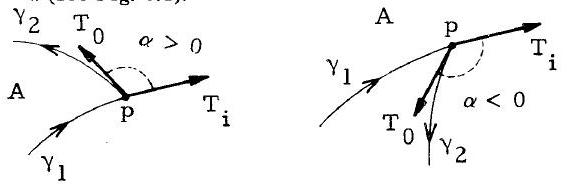
\includegraphics[max width=\textwidth]{2022_07_16_f4e476ee2159dc67e746g-56}

Fig. 8.1 Corner Angles In the proof of the Gauss-Bonnet formula that follows, the differential geometry involved is simple. The crux of the theorem is the Hopf Umlaufsatz (see discussion after proof). As usual, a simple closed curve is a homeomorphic image of the circle $S^{1}$ in $R^{2}$.

THEOREM (Gauss-Bonnet formula). Let $A$ be contained in a coordinate domain $U$ of $M$, let the bounding curve $\gamma$ of $A$ be a simple closed curve, and let $a_{1}, \ldots, a_{r}$ be the exterior corner angles of $\gamma$. Then

(1) $\int_{\gamma} k=2 \pi-\Sigma_{j=1}^{r} a_{j}-\int_{A} K$

where $k$ is the signed geodesic curvature function on $\gamma$ and $K$ is the Riemannian (Gaussian) curvature function on A.

Proof. Let $e_{1}, e_{2}$ be a $C^{\infty}$ positively oriented base field on $U$. Let $\gamma_{1}, \ldots, \gamma_{r}$ be the $C^{\infty}$ pieces of $y$ with each $\gamma_{j}$ paramet erized by arc length on the interval $\left[s_{j}, s_{j+1}\right], \gamma_{j}\left(s_{j+1}\right)=\gamma_{j+1}\left(s_{j+1}\right)$ for $j=1, \ldots, r-1$, while $\gamma_{f}\left(s_{r+1}\right)=\gamma_{1}\left(s_{1}\right)$, and $a_{j}$ the exterior corner angle at $\gamma\left(s_{j}\right)$. Let $T$ be the unit tangent to $\gamma$. By making a constant rotation of $e_{1}, e_{2}$ if necessary, we may assume $T\left(s_{1}+\right)=e_{1}$. Define $\zeta(s)$ on $\left[s_{1}, s_{2}\right]$ so $\zeta$ is $C^{\infty}, \zeta\left(s_{1}^{+}\right)=0$, and $T=\left(\cos \zeta e_{1}+(\sin \zeta) e_{2}\right.$. This $\zeta$ is well defined, since we have given its initial value and it is $C^{\infty}$, since locally it is given by $\zeta(s)=\cos ^{-1}<T(s), e_{1}(s)>$ for a proper branch of the inverse cosine. Thus we obtain $\zeta\left(s_{2}^{-}\right)$. Let $\zeta\left(s_{2}^{+}\right)=\zeta\left(s_{2}^{-}\right)+a$ and extend $\zeta$ to $\left[s_{2}, s_{3}\right]$ so $\zeta$ is $C^{\infty}$ and $T=\left(\cos \zeta e_{1}+(\sin \zeta) e_{2}\right.$, as before. Continuing this process, we extend $\zeta$ to $\left[s_{1}, s_{r^{+1}}\right]$ with $\zeta$ in $C^{\infty}$ at all interior points except $s_{i}$ where it has a jump precisely equal to $a_{i}$ for $i=2, \ldots, t$. Since $\gamma$ is a simple closed curve, we use the Hopf Umlaufsatz to obtain $\zeta\left(s^{-}\right)+a_{1}=\zeta\left(s_{1}^{+}\right)+2 \pi$. We include a schematic diagram (Fig. 8.2):

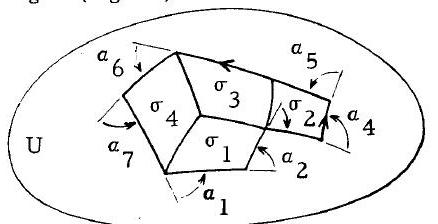
\includegraphics[max width=\textwidth]{2022_07_16_f4e476ee2159dc67e746g-57}

Fig. 8.2 Fundamental Set On each $C^{\infty}$ piece of $\gamma$ we have the positively oriented orthonormal base field, $T, N$, and the signed geodesic cirvature $k$ is defined by $D_{T} T=k N .$ In terms of $\zeta, T=(\cos \zeta) e_{1}+\left(\sin \zeta e_{2}\right.$, while $N=$ $(-\sin \zeta) e_{1}+(\cos \zeta) e_{2}$

Let $w_{1}, w_{2}$ be the dual l-forms to the base $e_{1}, e_{2}$, and let $w_{12}=$ $-W_{21}$ be the corresponding connexion 1-form on $U$ (note $w_{11}=w_{22}=0$ for the Riemannian connexion $D$ ). Thus $V=W_{1} \wedge_{2}$ is the volume element on $U$. Moreover, by the Cartan structural equations, $d w_{12}=$ $R_{12}$, and $K=\left\langle R\left(e_{1}, e_{2}\right) e_{2}, e_{1}\right\rangle=\left\langle\Sigma_{i=1}^{2} R{ }_{i 2}\left(e_{1}, e_{2}\right) e_{i}, e_{1}\right\rangle=R_{12}\left(e_{1}, e_{2}\right)$, thus $R_{12}=K W_{1} \wedge W_{2}$

Since $k=\left\langle D_{T} T, N>\right.$ and $D_{T} T=(T \zeta) N+(\cos \zeta)_{21}(T) e_{2}+$ $\left(\sin \zeta w_{12}(T) e_{1}\right.$, then

(2) $k=(T \zeta)-w_{12}(T)$

which is a Cartan formula for the geodesic curvature. Then
$$
\begin{aligned}
\int_{\gamma} k=\sum_{j=1}^{r} \int_{s} s_{j+1} \frac{d \zeta}{d s} d s-\int_{\partial c} w_{12}=& \sum_{j=1}^{r}\left[\zeta\left(s_{j+1}^{\infty}\right)-\zeta\left(s_{j}^{+}\right)\right]-\int_{c} d w_{12} \\
&=2 \pi-\sum_{j=1}^{r} \alpha_{j}-\int_{A} K,
\end{aligned}
$$
where we use Stokes' theorem for the second equality.//

The Gauss-Bonnet formula almost proves the Hopf Umlaufsatz (see Hopf ${ }^{1}$ ), which states if $y$ is a simple closed smooth $\left(C^{1}\right)$ curve in $R^{2}$, then $\int_{\gamma} k=\pm 2 \pi$, depending on the orientation of $\gamma$. We need the topological result that $y$ disconnects the plane into two components and the map $y$ may be extended to a homeomorphism of the interior of the disc $B(0,1)$, which then maps onto a set $A$, which is fundamental and has $y$ as bounding curve. Then letting $e_{1}=i_{2} e_{2}={ }^{\prime}$ (advanced calculus natation), we have $w_{12}=0, K=0$, and all $a_{i}=0$, so $\int_{\gamma} k=2 \pi$ if $y$ positively oriented. The reader may also be interested in the papers of $\mathrm{H}$. Whitney ${ }^{1}, \mathrm{~J} . \mathrm{S}$. Griffin, and $\mathrm{C}$. J. Titus.

The Gauss-Bonnet formula was first proved by Bonnet in $1848 .$ Somewhat earlier Gauss had proved the following result on geodesic triangles. THEOREM (Gauss). Let $A$ be a fundamental set of $M$ bounded by three (non-closed) geodesics, i.e., $A$ is a geodesic triangle, and let $\beta_{1}, \beta_{2}$, and $\beta_{3}$ be the interior angles at the corners. Then $\int_{A} K=$ $\beta_{1}+\beta_{2}+\beta_{3}-\pi$, and this number is called the excess of the triangle.

Proof. The Gauss-Bonnet formula is applicable. Since $k=0$ and $\alpha_{i}=\pi-\beta_{i}$, we have $0=2 \pi-\Sigma_{1}^{3}\left(\pi-\beta_{j}\right)-\int_{A} K . / /$

Corollary. Let $B$ be the sum of the interior angles of a geodesic triangle $A$ on $M$. Then $B$ is $>\pi,=\pi$, or $<\pi$, according as $K>0,=0$, or $<0$ on $A$. If $K$ is constant and not zero on $A$, then the area of $A$ equals the excess of $A$ divided by $K$.

We obtain some simple applications of the Gauss-Bonnet formula by applying it to the cases when $M$ is diffeo to the sphere or the torus. In the former case $\int_{M} K=4 \pi$, and in the latter case $\int_{M} K=0$. These are special cases of the Gauss-Bonnet theorem which we prove later in this section. We sketch the proofs of these facts.

When $M$ is diffeo to $S^{2}$, we let $y$ be the image of the equator (under the diffeo), $A_{1}$ the image of the "northern" hemisphere, and $A_{2}$ the image of the "southern" hemisphere (see Fig. 8.3). Supposing $y$ to be the bounding curve of $A_{1}$, we have
$$
\int_{\gamma} k=2 \pi-\int_{A_{1}} K \text { and } \int_{-\gamma} k=-\int_{\gamma} k=2 \pi-\int_{A_{2}} K .
$$
Hence $\quad \int_{M} K=\int_{A_{1}} K+\int_{A_{2}} K=4 \pi$.

When $M$ is diffeo to the torus, let $A_{1}$ be the image of the "top half" and $A_{2}$ the image of the "bottom half" of the torus so $A_{1}$ and $A_{2}$ are bounded and separated by the image $\gamma$ of the "inside" and "outside" curve on the torus (see Fig. 8.3). Again letting $\gamma$ be the bounding curve of $A_{1}$, connecting and closing $\gamma$ via a cut curve $\beta$ (see Fig. 8.3), and taking a limit, we obtain $\int_{\gamma} k=2 \pi-2 \pi-\int_{A} K$ and $-\int_{\gamma} k=-\int_{A} K$ so $\int_{M} K=0$.

Our next task is to free the Gauss-Bonnet formula from the special neighborhood $U$. The proof follows the notes of Samelson. Define the Euler characteristic, $X_{c}(A)$, of $A$ with respect to c by ${ }_{c}(A)=$ $V-E+F$, where $V$ is the number of vertices of $c$, $E$ the number of\\

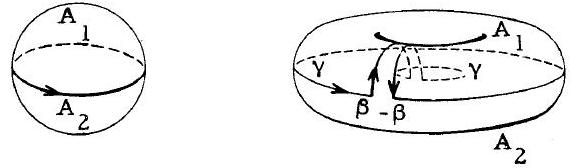
\includegraphics[max width=\textwidth]{2022_07_16_f4e476ee2159dc67e746g-58}

Fig. $8.3$ Sphere and Torus

edges, and $F$ the number of faces.

THEOREM. Let A be a fundamental set on $M$, let the bounding curve $\gamma$ of $A$ be a finite disjoint union of simple closed curves, and let $a_{1}, \ldots, a_{r}$ be the exterior corner angles of $\gamma_{0}$ Then

(3) $\int_{\gamma} k=2 \pi \mathcal{X}_{c}(A)-\Sigma_{i=1}^{r} \alpha_{i}-\int_{A} K$.

This expression proves $X_{c}(A)$ is independent of $c$, so define $\mathfrak{X}(A)=$ $X_{c}(A)$ to be the Euler characteristic of $A$ and drop the subscript c in the above formula.

Proof. Let $c=\sigma_{1}+\ldots+\sigma_{F}$ and note from the definition of a fundamental 2-chain we may apply the Gauss-Bonnet formula to each set $\left|\sigma_{j}\right|$ (for $\sigma_{j}$ defines a coordinate neighborhood of $\left|\sigma_{j}\right|$. Let $\alpha_{1}^{j}, \ldots, \alpha_{4}^{j}$ denote the four exterior angles for $\sigma_{j}$. Then
$$
\int_{\gamma} k=\Sigma_{j=1}^{F} \int \partial_{\sigma} k=\sum_{j=1}^{F}\left(2 \pi-\sum_{i=1}^{4} a_{i}^{j}\right)-\Sigma_{j=1}^{F} \int_{\sigma} K
$$
$$
\int_{\gamma} k=2 \pi F-\Sigma_{j=1}^{F} \Sigma_{i=1}^{4} a_{i}^{j}-\int_{A} K .
$$
Thus the problem is one of bookkeeping with the term $\Sigma \alpha_{i}^{j}$.

Let $\beta_{i}^{j}$ be the interior angle corresponding to each $\alpha_{i}^{j}$, thus $\beta_{i}^{j}=$ $\pi-\alpha_{i}^{j}$, and let $\beta_{s}=\pi-\alpha_{s}$ be the interior angles at the corners of $\gamma$. In the following we sum over $i=1, \ldots, 4$ and $j=1, \ldots, F$. The sum

\section{Notes on Differential Geometry}
$$
\begin{aligned}
\Sigma_{i j} \beta_{i}^{j}=2 \pi(V-r)+\Sigma_{1}^{r} \beta_{s}=2 \pi(V-r)+& \Sigma_{1}^{r}\left(\pi-a_{s}\right) \\
&=2 \pi V-\pi r-\Sigma_{1}^{r} \alpha_{s},
\end{aligned}
$$
since $r$ is the number of verticies of $c$ on $\gamma$ (as well as the number of angles and edges on $\gamma)$ so $(V-r)$ is the number of vertices interior to $A$, each of which contributes $2 \pi$ to the total sum.

We now show $r F=(2 E-r)$, which is the number of terms in the sum $\Sigma_{i j} \beta_{i^{*}}^{j}$ This is done by assigning to each $\beta_{i}^{j}$ an edge, namely, its "starting" edge, which is well-defined by the orientation. More precisely, if $T$ and $T^{\prime}$ are the unit vectors at the vertex of $\beta_{i}^{j}$ which are tangent to the edge curves of $\beta_{i}^{j}$, then $T$ and $T^{t}$ are independent, since $c$ is a fundamental chain, so $\left(\sigma_{j}\right)_{*}$ is non-singular on its domain (which is slightly larger than $I^{2}$ ). Thus $T$ is the "starting" edge of $\beta_{i}^{i}$ if and only if $T, T^{\prime}$ is a positively oriented bases (see Fig. 8.4).

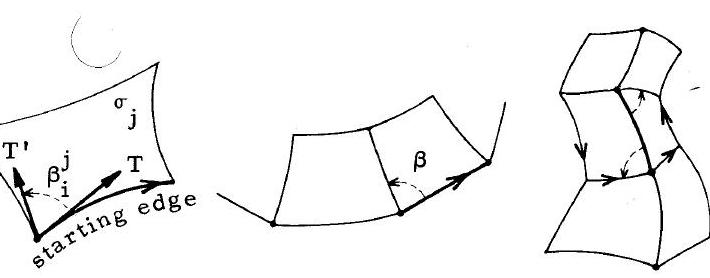
\includegraphics[max width=\textwidth]{2022_07_16_f4e476ee2159dc67e746g-59}

Fig. $8.4$ Starting Edges

Then each edge on the boundary $\gamma$ belongs to exactly one $\beta_{i}^{j}$, while each edge not on the boundary belongs to exactly two $\beta_{i}^{j}$ Thus $r F=$ $r+2(E-r)$, since $r$ is the number of edges on the boundary.

Finally,
$$
\Sigma_{i j} \alpha_{i}^{j}=\Sigma_{i j}\left(\pi-\beta_{i}^{j}\right)=\pi(2 E-r)-2 \pi V+\pi r+\sum_{1}^{r} a_{s}=2 \pi(E-V)+
$$

\section{Chap. 8 Gauss-Bonnet Theory and Rigidity}
Hence,
$$
\int_{\gamma} k=2 \pi(F-E+V)-\Sigma_{1}^{r} \alpha_{s}-\int_{A} K \cdot / /
$$
GAUSS-BONNET THEOREM. Let $M$ be a compact connected oriented Riemannian 2-manifold with Riemannian (Gaussian) curvature frinction $K$. Then $\int_{M} K=2 \pi \mathfrak{X}(M)$.

Proof. We apply the preceding theorem to a fundamental chain on $M$ which will have no boundary and no exterior angles. $/ /$

The above theorem is an important example of a theorem relating differential geometry and topology. The Euler characteristic is a topological invariant which does not depend on either the differentiable structure or the Riemannian structure on $M$. The theorem may be used to prove many "negative" statements: for example, there does not exist a Riemannian metric on the torus with $K>0$ everywhere (nor does there exist one with $K<0$ everywhere) since $\mathfrak{X}(M)=0$ (which we computed above for the induced Riemannian metric). The theorem has been generalized for dimensions greater than two and provides one of the first successes of the global theory of fiber bundles.

\section{Section $8.2$ Index theorem.}
This section is also based on the notes of Samelson. Let $n=2$ and let $W$ be a $C^{\infty}$ vector field on $M$. If $W=0$, then $m$ is a singularity of $W$. Assuming $W$ has only isolated singularities, we define the index of $W$ at $m, J(W, m)$, as follows.

Let $U$ be a coordinate domain, with coordinate radius $b>\dot{0}$, about $m$ with $W \neq 0$ on $U-[m]$. Assume the coordinate map is orientation preserving, and let $\sigma_{t}$ be the oriented coordinate circle of radius $r$ about $m$ with $0<r<b$ and $\sigma_{r}$ defined on $[0,1]$. Let $X$ be a unit vector field on $U$. Since $W$ does not vanish on $\sigma_{r}$, by using the proper inverse cosine function one obtains a $C^{\infty}$ function $\theta$ on $[0,1]$ with $\langle W(s), X(s)\rangle=|W(s)| \cos \theta(s)$ on $[0,1]$. Let

(4) $2 \pi J_{X}\left(W, m, r_{,}\right)=\theta(1)-\theta(0)$.

For $0<r<b, J_{X}(W, m, r)$ is a continuous integer-valued function, and hence ylelds a constant $J_{X}(W, m)$. If $m$ is not a singular point,

\section{2}
then for small $r>0, \theta$ is close to the constant $\cos ^{-1}\left(\left\langle W_{m}, X_{m}\right\rangle /\right.$ $\left\{W_{m} \mid\right)(\bmod 2 \pi)$; hence $\theta(1)=\theta(0)$ and $J_{X}(W, m)=0$. If $Y$ is another unit vector field on $U$, then
$$
J_{X}(W, m)=J_{Y}(W, m)+J_{X}(Y, m)=J_{Y}(W, m)
$$
since $Y$ has no singularities. Thus $J_{X}(W, m)$ is independent of $X$. An analogous argument shows $J(W, m)$ can be computed by using any simple closed $C^{\infty}$ curve $\sigma$ about in with $\sigma$ in $U$, and thus $J(W, m)$ is an integer depending only on $W$ and $m$ (see Fig. 8.5).\\

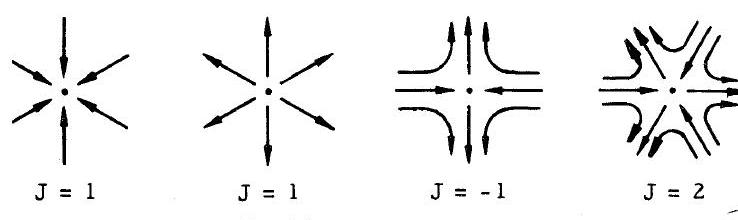
\includegraphics[max width=\textwidth]{2022_07_16_f4e476ee2159dc67e746g-60}

Fig. 8.5 Examples of $J(W, m)$

If $W$ has only a finite number of singularities, define the index of $W, J(W)$, by $J(W)=\Sigma_{m} J(W, m)$

INDEX THEOREM. If $M$ is a compact connected oriented Riemannian 2-manifold and $W$ is a $C^{\infty}$ vector field on $M$ with a finite number of singularities, then the index of $W$ equals the Euler characteristic of $M$.

Proof. Take an oriented fundamental chain $\mathrm{c}=\sigma_{1}+\cdots+\sigma_{\mathrm{r}}$ with at most one singularity $m_{i}$ of $W$ in the interior of each $\left|\sigma_{i}\right|$. Let $\gamma_{i}$ be the bounding curve of $\sigma_{i}$ and define functions $\theta_{i}, \zeta_{i}$ and $\xi_{i}$ on the domain of $\gamma_{i}$ so $\theta=\zeta_{i}+\xi_{i}, \theta_{i}$ is an angle between $W$ and $e_{i}, \zeta_{i}$ is an angle between the tangent $T_{i}$ of $\gamma_{i}$ and $e_{1}$, and $\xi_{i}$ is an angle between $W$ and $T_{i}$. The functions $\theta_{i}, \zeta_{i}$, and $\xi_{i}$ will be piece-wise $C^{\infty}$ and $\theta_{i}$ is continuous. By integrating over the pieces of $\gamma_{i}$ we obtain

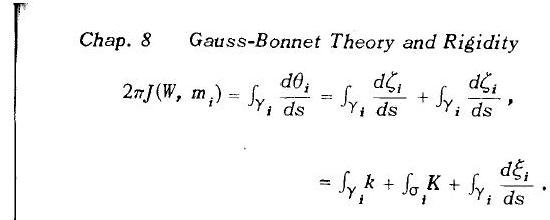
\includegraphics[max width=\textwidth]{2022_07_16_f4e476ee2159dc67e746g-60(1)}

Adding over the 2-cubes in $c$ gives

(5) $2 \pi J(W)=\int_{M} K$

since the integrals over the bounding curves cancel one another. By the Gauss-Bonnet theorem, $J(W)=X(M) . / /$

Omitting the last line of the proof, we note $2 \pi J(W)=\int_{M} K$ implies $J(W)$ is independent of $W$ as long as $W$ has only a finite number of singularities. Then for any oriented fundamental chain $\mathrm{c}$ we can define a particular $W$ which has a singularity for each face, edge, and vertex with index $1,-1$, and 1 , respectively. We indicate in Fig. $8.6$ how $W$ is defined on each 2-cube. Actually $W$ would be precisely defined by defining a field on a neighborhood of $I^{2}$ and carrying this to each $\left|\sigma_{i}\right|$ via the map $\sigma_{i}$.

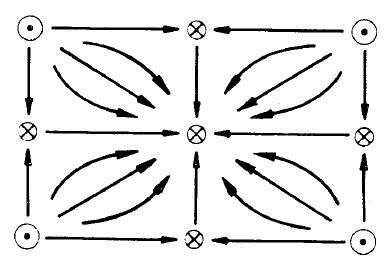
\includegraphics[max width=\textwidth]{2022_07_16_f4e476ee2159dc67e746g-60(2)}

Fig. $8.6$ The Canonical Vector Field on a 2-cube

Thus $W$ is defined by "going out from each vertex and in to the center of each face." From Fig. $8.6$ we see $J(W)=V-E+F=X_{c}(M)$. Thus we again prove $X_{c}(M)$ is independent of $c$, and $2 \pi^{\circ}(M)=2 \pi J(W)=$ $\int_{M} K$ reproves the Gauss-Bonnet theorem. Corollary. If $M$ is a manifold as described in the theorem and there exists a non-vanishing $C^{\infty}$ vector field on $M$, then $\mathscr{X}(M)=0$. Thus any surface that is diffeomorphic to the 2 -sphere has no nonvanishing $C^{\infty}$ vector fields.

Actually, a differentiable manifold (any dimension) admits a nonzero continuous vector field if and only if its Euler characteristic is zero (see Steenrod, p. 203, and Alexandroff and Hopf, p. 549).




Problems.

\begin{enumerate}
  \setcounter{enumi}{75}
  \item Prove that the volume $V_{n}$ of the unit sphere in $R^{n+1}$ is equal to $2^{n+1} \pi^{k} k ! / n !$ for even $n=2 k$ 76. If $M$ is a compact surface in $R^{3}$ with constant mean curvature and $y_{3}>0$ on $M$, show $M$ is a sphere (see section $8.5$ ).

  \item If $f$ is an isometry between two oriented surfaces in $R^{3}$ of positive Gaussian curvature which preserves the third fundamental form, show the surfaces are congruent or symmetric.

  \item Use an integral argument to show there exists no compact minimal surface in $R^{3}$.

\end{enumerate}
\section{Existence Theory}
Section 9.1. Involutive distributions and the Frobenius theorem.

We prove the standard theorem on the existence of “integral manifolds ${ }^{n}$ of a distribution following Chevally (p.88). The theorem also appears in Auslander and Mackenzie (p. 147) with the terminology altered slightly.

In this section let $M$ be a $C^{\infty} n$-manifold. A $k$-dimensional distribution on a set $A$ in $M$ is a function $P$ that assigns to each point $p$ in $A$ a $k$-dimensional subspace $P$ of the tangent space $M$. We say $P$ is $C^{\infty}$ on $A$ if $A$ is open, and for each $p$ in $A$ there are $k$ independent $C^{\infty}$ vector fields $X_{1}, \ldots, X_{k}$ which span $P_{m}$ for all $m$ in some neighborhood of $p$. A vector field $X$ with domain $B$ lies in $P$ or is in $P$ if $B \subset A$, and $X$ is in $P$ for all $p$ in $B$. A $C^{\infty}$ distribution $P$ is integrable (involutive or closed) when it is closed under the bracket operation, i.e., if $X$ and $Y$ are any $C^{\infty}$ fields with common domain that lie in $P$, then $[X, Y]$ lies in $P . A$ submanifold $V$ of $M$ is an integral submanifold or integral manifold of $P$ if $V$ is contained in the domain of $P$, and $V=P$ for all $p$ in $V ;$ thus the subspace of the tangent space $M_{p}$ which belongs to $V_{p}$ is exactly the subspace $P_{p}$.

The theorem proved below implies a $C^{\infty}$ distribution has integral manifolds if and only if it is involutive. A slightly stronger statement is made involving the existence of a special coordinate system. First some terminology: if $x_{1}, \ldots, x_{n}$ is a coordinate system on $M$ with domain $U$, then define a slice of $U$ to be any subset of $U$ on which $t$ of the functions $x_{1}, \ldots, x$ are constant, where $1 \leqslant r<n$. Obviously, each slice of $U$ is a submanifold of $U$ (or $M$ ). THEOREM. Let $P$ be a $k$-dimensional involutive $C^{\infty}$ distribution on $M$. For any $m$ in $M$ there exists a coordinate system $x_{1}, \ldots, x_{n}$ with domain $U$ including $m$ such that the coordinate fields $\partial / \partial x_{j}$ for

$j=1, \ldots, k$ span $P$ at each point of $U$. Thus the slices of $U$ of which $x_{k+1}, \ldots, x_{n}$ are constant are integral manifolds of $P$.

The theorem is proved by induction on $k$. The case $k=1$ is covered by the following lemma, and note in this case any distribution is automatically involutive.

LEMMA. If $X$ be a $C^{\infty}$ vector field on $M, p$ in $M$, and $X, 0$, then there exists a coordinate system $y_{1}, \ldots, y_{n}$ on a neighborhood $U$ of $p$ with $X=\partial / \partial y_{1}$ on $U$.

Proof (of lemma). Let $x_{i}=u_{i}$ o $\phi$ be a coordinate system on the neighborhood $V$ of $p$ with $x_{i}(p)=0$ and $\partial / \partial x_{1}(p)=X_{p}$. Let $X=$ $\sum_{1}^{n} a_{i}\left(\partial / \partial x_{i}\right)$ where $a_{i}$ are $C^{\infty}$ real valued functions on $V$ and $a_{1}(p) \neq 0$, and restrict $V$ if necessary so $a_{1} \neq 0$ on $V$. Setting up the system of differential equations for the integral curves $\sigma$ of $X$ on $V$, we have
$$
\frac{d\left(x_{i} \circ \sigma\right)}{d t}=a_{i}^{\circ} \sigma \quad \text { or } \quad \frac{d f_{i}}{d t}=a_{i}\left(f_{1}(t), \ldots, f_{n}(t)\right)
$$
where $f_{i}(t)=x_{i} \circ \sigma(t)$. Applying an existence theorem from the theory of differential equations (Coddington and Levinson, Chapter 1) we obtain an $r>0$ and $n$ functions $F_{i}\left(t, a_{1}, a_{2}, \ldots, a_{n}\right)$ which are $C^{\infty}$ on the neighborhood $W$ of the origin in $R^{n+1}$ where $|t|<r$ and $\left|a_{i}\right|<r$ such that for $i=1, \ldots, n$ :

(1) $F_{i}\left(0, a_{1}, a_{2}, \ldots, a_{n}\right)=a_{i}$

(2) $\left(F_{1}(b), \ldots, F_{n}(b)\right)$ in $\phi(V)$ for $b$ in $W$,

(3) Letting $F\left(t, a_{2}, \ldots, a_{n}\right)=\phi^{-1}\left[F_{1}\left(t, 0, a_{2}, \ldots, a_{n}\right), \ldots, F_{n}\left(t, 0, a_{2, \ldots,}, a_{n}\right.\right.$ define a map $F$ of $B(0, r)$ in $R^{n}$ into $V$; then for fixed a ${ }_{2}, \ldots, a_{n}$ the curves
$$
\sigma_{\left(a_{2}, \ldots, a_{n}\right)}(t)=F\left(t, a_{2}, \ldots, a_{n}\right)
$$
are integral curves of $X, i_{*} e_{*}, F_{*}\left(\partial / \partial u_{1}\right)=X$. For points $\left(0, a_{2}, \ldots, a_{n}\right)$ in $B(0, r)$ we notice that $F\left(0, a_{2}, \ldots, a_{n}\right)=$ $\phi^{-1}\left(0, a_{2}, \ldots, a_{n}\right) ;$ hence $F_{*}\left(\partial / \partial u_{i}\right)_{\text {origin }}=\partial / \partial x_{i}(p)$ for $i=2, \ldots, n$. Since $F_{*}\left(\partial / \partial u_{1}\right)_{b}=X_{F(b)}$ for all $b$ in $B(0, r)$ we have $\left.F_{*}=(\phi-1)\right)_{*}$ the origin in $R^{n}$. Hence $F$ is non-singular at the origin and by the Inverse Function Theorem $F$ is a diffeo between a neighborhood of the origin and a neighborhood $U$ of $p$ with $U \subset V$. Finally, let $y_{i}=u_{i} \circ F^{-1}$ on $U_{.} /$

Intuitively, in the above proof we have changed the $x_{1}, \ldots, x_{n}$ coordinates about $p$ by leaving the slice where $x_{1}=0$ fixed, and replacing the " $x_{1}$-coordinate curves" by integral curves of $X$ emanating from this slice

Proof (of theorem). Take the point $m$ and take $C^{\infty}$ fields $X_{1}, \ldots, X_{k}$ that span $P$ on a neighborhood $U_{1}$ on $m$. Apply the previous lemma to get a coordinate system $y_{1}, \ldots, y_{n}$ about $m$ with domain $U_{2} \subset U_{3}$ such that $\partial / \partial y_{1}=X_{1}$ on $U_{2}$, and assume $y_{i}(m)=0$.

If $k=1$, then the coordinate system $y_{1}, \ldots, y_{n}$ satisfies the conclusion of the theorem. If $k>1$, we assume the theorem is true for distributions of dimension less than $k$, and we define the $(k-1)$ dimensional distribution $\bar{P}$ on $U_{2}$ by $\bar{P}=\left[X\right.$ in $\left.P: X y_{1}=0\right]$ for in $U_{2} .$ This is a $(k-1)$-dimensional $C^{\infty}$ distribution for it is spanned by the $(k-1)$ independent $C^{\infty}$ fields $Y_{i}=X_{i}-\left(X_{i} y_{1}\right) X_{1}$ for $i=2, \ldots, k$. It is involutive since if $Y$ and $Z$ are in $\bar{P}$, then $[Y, Z]$ is in $P$ and $[Y, Z]_{1}=Y\left(Z y_{1}\right)-Z\left(Y y_{1}\right)=0$ on $U_{2}$, so $[Y, Z]$ is in $\bar{P}$.

Let $V_{0}$ be the slice of $U_{2}$ defined by $y_{1}=0$. Then for $p$ in $V_{0}$, $\frac{P}{p} \subset\left(V_{0}\right)_{p}$, so we apply the induction hypothesis to the distribution $P$ on the manifold $V_{0}$ to obtain a coordinate system $z_{2}, \ldots, z_{n}$ on the neighborhood $U_{3}$ about $m$ in $V_{0}$ such that $\partial / \partial z_{2}, \ldots, \partial / \partial z_{k}$ span $\bar{P}$ on $U_{3} \cdot$ We define the map $\pi: U_{2} \rightarrow V_{0}$ by $\pi(p)=\phi^{-1}\left(0, y_{2}(p), \ldots, y_{n}(p)\right)$ where $\phi$ is the coordinate map so $y_{i}=u_{i} \circ \phi .$ Let $U_{4}=\pi^{-1}\left(U_{3}\right)$ and define functions $x_{1}, \ldots, x_{n}$ on $U_{4}$ by $x_{1}=y_{1}, x_{2}=z_{2} \circ \pi, \ldots, x_{n}=z_{n} \circ \pi$. Then the functions $x_{1}, x_{2}, \ldots, x_{n}$ define a coordinate system in a neighborhood $U$ of $m$ with $U \subset U_{4}$; indeed, $\partial / \partial \mathrm{x}_{1}(m)=\partial / \partial y_{1}(m)$, while $\partial / \partial x_{2}, \ldots, \partial / \partial x_{n} \operatorname{span}\left(V_{0}\right)_{m}$ at $m_{0}$

We show $\partial / \partial x_{1}, \ldots, \partial / \partial x_{k}$ span $P$ on $U$ by showing they span the same subspace as $X_{1}, Y_{2}, \ldots, Y_{k^{*}}$ Let $Y_{1}=X_{1}$, then we show $Y_{i}=0$ for $i=1, \ldots, k$ and $j=k+1, \ldots n$. Since $Y_{1}=X_{1}=\partial / \partial x_{i}$, we immediately

\section{Notes on Differential Geometry}
see $Y_{1} x_{j}=0$ for $j \neq 1$. Since $P$ is involutive, there are $C^{\infty}$ functions $g_{i r s}$ on $U$ such that for $i \leq k$ and $r \leq k$ we have $\left[Y_{i}, Y_{t}\right]=\sum_{s=1}^{k} \varepsilon_{i r s} Y_{s}$. Thus for $i=2, \ldots, k$ and $j>k, Y_{1}\left(Y_{i} x_{j}\right)=\left[Y_{1}, Y_{i}\right] x_{j}=\sum_{s=1}^{k} g_{1 i s}\left(Y_{s} x_{j}\right)$. This implies the functions $Y_{i} X_{j}$ satisfy a linear homogeneous system of ordinary differential equations along any $x_{1}$-curve. But on $V_{0}$, $x_{j}=z_{j}$ for $j>1$ and $Y_{i} x_{j}=Y_{i} z_{j}=0$ on $V_{0}$ for $j>k$ because of the choice of the coordinates $z_{2}, \ldots, z_{n}$. Hence, by the uniqueness of solu tions to systems of the above type, $Y_{i} x_{j}=0$ for $i \leq k$ and $j>k . / /$


Section 9.2. The fundamental existence theorem for hypersurfaces.

Let $U$ be an open set in $R^{n}$ on which is defined real valued $C^{\infty}$ functions $g_{i j}$ and $b_{i j}$ for $1 \leq i, j \leq n$ such that the matrices $\left(g_{i j}\right)$ and $\left(b_{i j}\right)$ are symmetric and $\left(g_{i j}\right)$ is positive definite. Roughly speaking, we prescribe conditions which imply the existence of a coordinate system on a hypersurface of $R^{n+1}$ such that the matrices $\left(g_{i j}\right)$ and $\left(b_{i j}\right)$ are the coordinate representations of the first and second fundamental forms, respectively. We demand that $\left(\xi_{i j}\right)$ and $\left(b_{i j}\right)$ satisfy the Gauss curvature and Codazzi-Mainardi equations, and explain this demand. On $U$, define functions $\Gamma_{j k}^{i}$ in terms of the $g_{i j}$ by the classical formula (see section 6.2), and define functions $w_{i j}\left(e_{k}\right)=\Gamma_{j k^{s}}^{i}$ $W_{n+1 j}\left(e_{k}\right)=-b_{i k}, W_{j n+1}\left(e_{k}\right)=\sum_{r=1}^{n}\left(g^{-1}\right)_{i r} b_{r k}$, and $W_{n+1 n+1}\left(e_{k}\right)=0$, for all $i, j, k \leq n$. Then if there was a coordinate system with coordinate fields e $e_{1} \ldots e_{i 2}$ whose image set was $U$, the Gauss curvature equations and Codazzi-Mainardi equations imply (see section 6.6)

(1) $d w_{i j}\left(e_{r}, e_{s}\right)=-\sum_{k=1}^{n+1} w_{i k} \wedge w_{k s}\left(e_{r^{2}} e_{s}\right)$

and

(2) $d W_{j n+1}\left(e_{r^{\prime}} e_{s}\right)=-\sum_{k=1}^{n} W_{j k} \wedge W_{k n+1}\left(e_{r}, e_{s}\right)$ respectively. Thus we say $\left(\xi_{i j}\right)$ and $\left(b_{i j}\right)$ satisfy the Gauss curvature and Codazzi-Mainardi equations if (1) and (2) hold for the functions defined on $U$ where the left sides are computed by $d w(e, e)=$ $\left.1 \partial / \partial u_{t}\right) w_{i j}\left(e_{s}\right)-\left(\partial / \partial u_{s}\right) w_{i j}\left(e^{2}\right)$, etc.

THEOREM. Let $\left(g_{i j}\right)$ and $\left(b_{i j}\right)$ be defined on $U$ as described above and suppose they satisfy the Gauss curvature and CodazziMainardi equations. Then for any point $p$ in $U$, there is a neighbor hood $V \subset U$ and a $C^{\infty} \operatorname{mapping} F: V \rightarrow R^{n+1}$ such that $F(V)$ is an $n=d i m e n$ sional submanifold of $R^{n+1}, F-1$ is a coordinate map on $F(V)$, and $(g$, and $\left(b_{i j}\right)$ are the coordinate representation matrices of the first and second forms on $F(V)$, respectively.

Proof. Let $u_{1}, \ldots, u_{n}$ be the natural coordinate functions on $U$. We seek $(n+1) R^{n+1}$-valued functions $e_{1} \ldots, e_{n+1}$ defined on $U$ that satisfy the Gauss equations and Weingarten equations, i.e.,


\section{Chap. $9 \quad$ Existence Theory}
\section{Section 9.3. The exponential map.}
Let $D$ be a connexion on $M^{n}$. From section $5.1$ we know for each vector $X$, tangent to $M$ at $m$, there is unique geodesic $g_{X}(t)$ of the connexion $D$, which is defined on a neighborhood of zero in $R$ with $g_{X}(0)=m$ and tangent $X$ at $t=0$. Furthermore, for appropriate $s$ in $R, g_{s X}(t)=g_{X}(s t)$ by the nature of the differential equations defining the geodesics. This implies that $\mathscr{g}_{a X}(1)$ is defined if $g_{X}(a)$ is defined, thus $g_{Y}(1)$ is a well-defined point of $M$ for $Y$ near zero in $M_{m}$

Definifion. For $Y$ in $M_{m}$, we define $\exp _{m} Y=g_{Y}$ (1) when the latter is defined. The map exp $\mathrm{ex}_{m}$ is called the exponential map.

The name "exponential map" is used because in a special case for the general linear group $G L(n, R)$ it becomes the classical map, $A \rightarrow e^{A}=I+A+\left(A^{2} / 2 !\right)+\ldots$, from the set of all $n$ by $n$ real matrices into the set of non-singular matrices (problem 81).

Our current objective is to obtain some important properties of the exponential map and to state these precisely we must use the tangent bundle $T(M)$ of $M$

Proposition 1. Let $N$ be the subset of $T(M)$ such that if $(m, Y)$ in $N$ then $\exp _{m}(Y)$ is defined and define the map exp: $N \rightarrow M$ by $\exp (m, Y)=\exp _{m}(Y) .$ Then $N$ is an open set and $\exp$ is $C^{\infty}$ on $N .$ In particular let $\hat{M}=[(m, 0)$ in $T(M): m$ in $M]$, then there is an open set $\widehat{N}$ in $T(M)$ such that $\hat{M} \subset \widehat{N} \subset N$

Proof. We do not completely prove the above proposition. Applying the local theory of differential equations we prove the last statement of the theorem and we prove exp: $N \rightarrow M$ is $C^{\infty}$. Then we

sketch the proof that exp is $C^{\infty}$ on $N$ and refer the reader to Lang.

Using the above notation, if $g(t)$ is a geodesic in the neighborhood $U$, then
$$
\frac{d^{2}\left(x_{k} \circ g\right)}{d t^{2}}+\sum_{i, j=1}^{n} \Gamma_{i j}^{k} \frac{d\left(x_{i} \circ g\right)}{d t} \frac{d\left(x_{j} \circ g\right)}{d t}=0
$$
for $t$ such that $g(t)$ in $U$. For each point $(m, 0)$ in $T(M)$ take a coordinate neighborhood $U_{m}$ of $m$ in $M$ and apply the existence and uniqueness the orem to the above differential equation to obtain a real number $b>0$, a neighborhood $V_{m}$ of $(m, 0)$ in $T(M)$ with $V_{m} \subset \pi^{-1}\left(U_{m}\right), a^{\infty}$ map $g:(-b, b) \times V_{m} \rightarrow M_{\text {。 }}$ such that for fixed $(p, Y)$ in $V_{m}$, the curve $g_{Y}(t)=g(t ; p, Y)$ is the unique geodesic defined on $(\ldots b, b)$ which passes through $p$ with tangent $Y$ at $t=0$. Morenver, for $(p, Y)$ in $V$ m and $a>0$, we have $g_{a Y}$ defined on $(-b / a, b / a)$, since $g_{a Y}(t)=$

$g_{Y}(a t)=g(a t ; p, Y) .$ Choose $a>0$ so $a<b$ and let $W_{m}=\left[(p, X)\right.$ in $V_{m}$ : $(p, X / a)$ in $\left.V_{m}\right]$. Then for $(p, X)$ in $W_{m}, \exp (p, X)=g(1 ; p, X)=$

$g(a ; p, X / a)$ is defined and exp is $C^{\infty}$ on $W m^{\circ}$

Let $N=U_{m} W_{m}$, and the last sentence of the theorem is proved.

For each $(p, Y)$ in $T(M)$, choose $a>0$ so $(p, a Y)$ in $\hat{N}$, and thus $g_{Y}(t)$ is defined in some neighborhood of $t=0$. As usual, for any curve $g$ let $T_{g}$ be its tangent vector and define the natural lifting of a curve $g$ in $M$ to a curve $\bar{g}$ in $T(M)$ by $\bar{g}(t)=\left(g(t), T_{g}(t)\right)$. Now define a global vector field $Z$ on $T(M)$ by $Z(p, Y)=T_{\bar{g}}(0)$. Then $Z$ is a

$C^{\infty}$ field on $T(M)$ by the above analysis, and if $\frac{Y}{\sigma}$ is an integral curve of $Z$, then $\pi \circ \sigma$ is a geodesic in $M$. The field $Z$ is called the geodesic flow field associated with the connexion. The fact that exp is $C^{\infty}$ on all of $N$ now follows from Theorem 5 on p. 66 in Lang. $/ /$

Corollary 1. For fixed $p$ in $M$, the map exp$p_{p}$ is a diffeo of a neighborhood of 0 in $M_{p}$ onto a neighborhood of $p$. Furthermore, if $\eta_{0}$ : $M_{p} \rightarrow\left(M_{p}\right)_{0}$ is the natural map of the tangent space at $p$ onto its tangent space at 0 , then $\left.(\exp )_{p}\right)_{*} \circ \eta_{0}$ is the identity $\operatorname{map}$ on $M_{p}$.

Proof. The map $\eta_{0}$ is defined by choosing any base $e_{1}, \ldots, e_{n}$ of $M_{p}$ and letting $z_{1}, \ldots, z_{n}$ be its dual base. Then $z_{1}, \ldots, z_{n}$ are a global coordinate system on the vector space viewed as a $C^{\infty}$ manifold. Let $\eta_{0}\left(e_{i}\right)=\left(\partial / \partial z_{i}\right)_{0}$ for all $i$. This map $\eta$ is independent of the particular base $e_{1}, \ldots, e_{n}$; furthermore, by evaluating the global fields $\partial / \partial z_{i}$ at any point $Y$ in $M_{m}$, we obtain a natural isomorphism $\eta_{Y}: M \rightarrow\left(M_{p}\right)$ In these notes, for any $X$ in $M_{p}$ we let $\bar{X}$ be the natural constant vector fiela on $M_{p}$ associated with $X$, where $\vec{X}_{\boldsymbol{Y}}=\eta_{Y}(X)$.

Take $X$ in $M_{p}$, then $\eta_{0}(X)=\bar{X}_{0^{\circ}}$ To compute $\left(\text { exp} p_{p}\right)_{*} \bar{X}_{0}$ we note $\bar{X}_{0}$ is the tangent vector at $t=0$ to the ray $\gamma(t)=t X$ in $M_{p}$ The curve $\exp _{p} \circ \gamma(t)=\exp _{p} t X$ is by definition the geodesic through $p$ with tangent $X$ at $t=0$. Thus $\left(\exp _{p}\right)_{*} \bar{X}_{0}=X$. Thus $\left(\exp p_{p}\right)_{*}$ is non-singular and onto at the origin in $M_{p^{*}}$ The corollary now follows by applying the Inverse Function theorem.//

\section{Chap. 9 Existence Theory}
Corollary 2. Let $G: \widehat{N} \rightarrow M \times M$ by $G(p, Y)=\left(p, \exp _{p} Y\right)$. Then $G$ is $C^{\infty}$ and $G_{*}$ is non-singular and onto at all points $(p, 0)$ in $T(M)$.

Proof. Let $\pi_{i}: M \times M \rightarrow M$ by $\pi_{i}\left(m_{1}, m_{2}\right)=m_{i}$ for $i=1,2$. Each $\pi_{i}$ is $C^{\infty}$. Since $\pi_{1} \circ G=\pi_{1}$ and $\pi_{2} \circ G=\exp$, the map $G$ is $C^{\infty}$ on $\hat{N}$.

The tangent space $\hat{N}_{(p, 0)}$ is naturally isomorphic to $M_{p} \times\left(M_{p}\right)_{0}$, while the tangent space to $M \times M$ at $G(p, 0)=(p, p)$ is naturally isomorphic to $M_{p} \times M_{p^{*}}$. In terms of these natural isomorphic spaces, $G_{*}$ is the identity on the first factor and $\left(e x p_{p}\right)_{*}$ on the second factor Hence, by Corollary $1, G_{*}$ is non-singular at $(p, 0) . / 1$

We apply Corollary 1 to obtain normal coordinate systems. For any $m$ in $M$ let $e_{1}, \ldots, e_{n}$ be a base of $M_{m}$, let $z_{1}, \ldots, z_{n}$ be its dual base, and let $\bar{U}$ and $U$ be neighborhoods of $O$ in $M_{m}$ and $m$ in $M$, respectively, such that exp $\operatorname{ex}_{m}$ is a diffeo of $\bar{U}$ onto $U$ whose inverse we denote by exp ${ }^{-1}$. Then define $C^{\infty}$ functions $z_{i}$ exp ${ }^{-1}$ for alli. These functions $x_{1}$ in $x_{n}$ define a $x_{i}=$ ordinate system (of the connexion $D$ ) on $U .$ ordinate system (of the connexion $D$ ) on $U$. The curves $\sigma$ in $U$ such that $x_{i} \circ \sigma(t)=a_{i} t$ for constants $a_{1}, \ldots, a_{n}$, are geodesics emanating from $m($ at $t=0)$, and if $\Gamma_{j k}^{i k}$ are the connexion functions on $U$ for this coordinate system, then $\Gamma_{j k}^{i}(m)=0$, provided the connexion has zero

One verifies this last statement by letting $X_{i}=\partial / \partial x_{i}$ and then $D_{X}\left(X_{j}\right)=\sum_{k=1}^{n} \Gamma_{j i}^{k} X_{k}$ by definition of $\Gamma_{j i}^{k}$. Since the curve $\sigma$ with $x_{i} \circ \sigma(t)=t, x_{j} \circ \sigma(t)=t$, and $x_{k} \circ \sigma(t)=0$ for $k \neq i$ or $j$, is a geodesic, its tangent $X_{i}+X_{j}$ satisfies the condition $0=D_{\left(X_{i}+X_{j}\right)}\left(X_{i}+X_{j}\right)=$ $D_{X_{i}} X_{i}+D_{X_{i}} X_{j}+D_{X_{j}} X_{i}+D_{X_{j}} X_{j^{*}}$ Thus at $m_{p} D_{X_{i}} X_{i}=0$ for all $i_{2}$ since each coordinate curve emanating from $m$ is a geodesic, and if $D$ has zero torsion, then $0=2\left(D_{X_{i}} X_{j}\right)_{m}=2 \sum_{k} \Gamma_{j i}^{k}(m) X_{k}$ so $\Gamma_{j i}^{k}(m)=0$ for all $i, j$, and $k$.

We apply Corollary 2 to obtain Fermi coordinates along a curve. Let $\sigma$ be a $C^{\infty}$ curve in $M$ that is univalent on the open interval $I \subset R .$ Let e $e_{1}, \ldots, e_{n}$ be $C^{\infty}$ fields on $\sigma$ that are independent at each $\sigma(t)$ and $e_{n}(t)=T_{\sigma}(t)$ for all $t$ in $l$. Let $z_{1} \ldots, z_{n}$ be the dual base to $e_{1}, \ldots, e_{n}$ for each $t .$ By Corollary 2, there is a neighborhood $V$ of $\hat{M} \subset T(M)$ such that $G$ is a diffeo of $V$ onto a neighborhood $N_{M}$ of the diagonal in $M \times M$. Let $U=\left[(m, Y)\right.$ in $V: m=\sigma(t)$ and $z_{n}(Y)=0$ for some $t$ in $I]$. Then $F=\left.G\right|_{U}$ is a 1 to $1 C^{\infty}$ map of the submanifold $U$ into $M \times M$. Moreover $F_{*}$ is non-singular at each point of $U_{,}$so $F$ is an imbedding of $U$ into $M \times M$. The map $H=\pi_{2} \circ F$ then gives a 1 to $1 C^{\infty}$ map of $U$ onto an open neighborhood $W$ of the image set $\sigma(I)$. Define Fermi coordinate $y_{1}, \ldots, y_{n}$ on $p$ in $W$ by letting $H^{-1}(p)=$ $(o(t), Y)$ in $W$ and $y_{i}(p)=z_{i}(Y)$ for $i=1, \ldots, n-1$ and $y_{n}(p)=t$.

More special types of Fermi coordinates can be defined by taking $e_{1}, \ldots, e_{n}$ to be a parallel base along a geodesic $\sigma$, and in the Riemannian case, one can take an orthonormal parallel base along a geodesic.

Section 9.4. Convex neighborhoods.

This section is devoted to proving the following theorem, due to J. H. C. Whitehead.

THEOREM. Let $M$ be a $C^{\infty}$ manifold and $D$ be a $C^{\infty}$ connexion on $M$. Then for any point $m$ in $M$ there is a neighborhood $U$ of $m$ which is convex; i.e., for any two points in $U$ there is a unique geodesic of $D$ which joins the two points and lies in $U$.

Proof. We may assume $D$ has zero torsion, since by section $5.4$ there is a unique torsion-free connexion with the same geodesics. The theorem is local, and we work completely in one coordinate neighborhood of $m$. From the previous section we choose a normal coordinate system $x_{1}, \ldots . x_{n}$ about $m$ with domain $A$, thus $x_{i}(m)=0$ and $\Gamma_{j k}^{i}(m)=0$ for all $i, j$, and $k$. Let $d(p, q)$ be a local metric on $A$ defined by $d(p, q)=\left[\Sigma_{t}\left(x_{i}(p)=x_{i}(q)\right)^{2}\right]^{1 / 2}, f(p)=d(p, m)$, and let $B(p, c)=[q$ in $A: d(p, q)<c]$ for $p$ in $A .$ Also for $p$ in $A$ and $X$ in $M_{p}$, let $|X|=$ $\left[\sum_{i} d x_{i}(X)^{2}\right]^{1 / 2}$

By Corollary 2 in section 3 , for each $p$ in $A$ there is a real number $r_{p}>0$ so that $G$ is a diffeo on the set $(q, X)$ where $q$ in $B\left(p, r_{p}\right)$ and $d\left(q, \exp _{p} X\right)<r_{p}$, Take $c>0$ so $\bar{B}=\bar{B}(m, c) \subset A .$ For each $p$ in $\bar{B}$ we obtain an integer $r_{p}>0$, The family of neighborhoods $B\left(p, r_{p}\right)$ for $p$ in $\bar{B}$ is a covering of the compact set $\bar{B}$, hence we may select a finite subcovering of neighborhoods belonging to $p_{1}, \ldots, p_{k}$. Let $s=\min \left[r_{1}, \ldots, r_{k}\right]$. Then for any $p$ in $\bar{B}^{\prime}$ exp maps a neighborhood $\bar{U}_{p}$ of the origin in $M_{p}$ diffeo onto $B(p, s)$. This follows since $p$ in $B\left(p_{j}, r_{i}\right)$ for some $j$ and hence $G$ is a diffeo on the set $(q, X)$ for $q$ in $B\left(p_{j}, r_{j}\right)$ and $d\left(q, \exp _{p} X\right)<r_{j \bullet}$ We fix $q=p$, and exp is a diffeo of

\section{Chap. 9 Existence Theory}
a neighborhood $\bar{V}_{p}$ of 0 in $M_{p}$ onto $B\left(p, r_{j}\right)$ and $s \leq r_{j *}$ We have proved the following:

LEMMA 1. For any $c>0$ with $\bar{B}(m, c) \subset A$, there exists an $s>0$ such that for $p$ in $\bar{B}(m, c)$ the map exp $p_{p}$ is a diffeo from a neighborhood $U_{p}$ of 0 in $\mathrm{M}_{p}$ onto $B(p, s) \subset A$.

We now prove two lemmas that complete the proof of the theorem.

LEMMA 2. There exists a real number $a, 0<a<1$ and $\bar{B}(m, a) \subset$ $A$, such that if $0<b<a$ and $g$ is a geodesic with tangent $T$ and $f \circ g(0)=b, T \& g(0)=0$, then $f \circ g$ has a strict relative minimum at $g(0)$. Thus if $g$ is tangent to the "sphere about m of radius $b^{\prime}$ at $g(0)$, then glies outside of $B(m, b)$ near $g(0)$.

Proof. We may assume $\left|T_{\varepsilon(0)}\right|=1$. Let $T=\sum_{j} a_{j} X_{j}$ where $X_{f}=$ $\partial / \partial x_{j}$ and $a_{j} \circ g=(d / d t)\left(x_{j} \circ g\right)$, and we assume 7 is extended to a $C^{\infty}$ field in a neighborhood of $g(0)$. Since $f=\left[\Sigma_{i} x_{i}^{2}\right]^{1 / 2}$ we have $T f=$ $\sum_{j} a_{j}\left(X_{j} f\right)=(1 / f) \Sigma_{j} a_{j} x_{j}$ and $T^{2} f=\sum_{k} a_{k}\left[\left(-x_{k} / f^{3}\right)\left(\sum_{j} a_{j} x_{j}\right)+(1 / f)\left(\Sigma_{j}\left(X_{k} a_{j}\right) x_{j}+\right.\right.$ $\left.a_{k}\right)$. At $t=0$, or at $g(0), T f=0 ;$ hence $T^{2} f=(1 / b)\left[\Sigma_{k} a_{k}^{2}+\sum_{k, j} a_{k} x_{j}\left(X_{k} a_{j}\right)\right]$ But at $g(0), \Sigma_{k} a_{k}^{2}=|T|^{2}=1$ and $\sum_{k} a_{k}\left(X_{k} a_{j}\right)+\sum_{r, s} \Gamma_{r s}^{j} a_{t} a_{s}=0$, since $g$ is a geodesic. Thus $T^{2} f=(1 / b)\left[1-\sum_{j, s} x_{j} \Gamma_{r}^{j} a_{s} a_{s}\right]$. Choose $a>0$ and $a<1$ so for points $p$ with $f(p) \leq a,\left|\Gamma_{j k}^{i}(p)\right|<1 / 2 n^{3}$ for all $i$, $j$, and $k$, which is possible since $\Gamma_{i k}^{i}$ continuous and $\Gamma_{j k}^{i}(m)=0$. Then at $g(0)$,
$$
\left|\Sigma_{j, r, s^{x_{j}}} \Gamma_{t s}^{j} a_{r} a_{s}\right| \leq\left(1 / 2 n^{3}\right)\left(\Sigma_{j, r, s}, 1\right) \leq 1 / 2,
$$
hence $T^{2} f(g(0))>0$, which implies $f \circ g$ has a strict relative minimum at $0.1 /$

LEMMA 3. Let a be given by Lemma 2 and apply Lemma l with $\mathrm{c}=\mathrm{a} / 2$ to obtain $\mathrm{s}>0$ with $s<(2 / 3) a .$ Then $B(m, s / 2)$ is convex.

Proof. Cloose any $p$ and $q$ in $B(m, s / 2)$. By lemma 1 there is a geodesic $g$ defined on some interval $[0, u]$ with $g(0)=p, \phi(u)=q$, and $g(t)$ in $B(p, s)$ for all $t$ in $[0, u]$. We show $f \circ g(t)<s / 2$ for all $t$ in $[0, u]$. Let $v$ be a number in $[0, v]$ where $f \circ g$ attains its maxim $t$ in value. Then $f \circ g(v)<a$ since $f \circ g(v)=d(m, g(v)) \leq d(m, p)+$ $d(p, g(v))<(s / 2)+s<g(v)=d(m, g(v)) \leq d(m, p)$ $d(p, g(v))<(s / 2)+s<a .$ Suppose $f \circ g(v) \geq s / 2 .$ Then $(f \circ g)^{\prime}(v)=0$ and $f \circ g(v)<a$ which implies by Lemma 2 that $f \circ g$ has a strict re- lative minimum at $v$ which gives a contradiction. Thus $B(m, s / 2)$ is convex.//

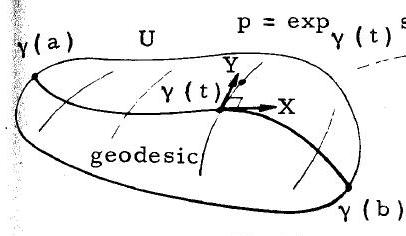
\includegraphics[max width=\textwidth]{2022_07_16_f4e476ee2159dc67e746g-72}

Fig. 9.1 Fermi Cordinates

Then for $(t, s)$ in $V, \phi^{-1}(t, s)=\exp _{\gamma(t)} s Y$. We let $X$ and $Y$ be the coordinate fields on $U$ which extend $X$ and $Y$ along $\gamma$. Since the $y$ curves are geodesics parameterized by arc length, $D_{\boldsymbol{Y}} \boldsymbol{Y}=0$ and $\langle Y, Y\rangle=1$, where $D$ is the Riemannian connexion. We compute $Y<X, Y\rangle=\left\langle D_{Y} X, Y\right\rangle+\left\langle X_{1} D_{Y} Y\right\rangle=\left\langle D_{Y} X, Y\right\rangle=1 / 2 X\langle Y, Y\rangle=0$, since the torsion is zero, so $D_{Y} X-D_{X} Y=[Y, X]=0$. Thus $\langle X, Y\rangle$ is constant along the $y$-curves and $\operatorname{since}\langle X, Y\rangle=0$ on $\gamma$ we have $\langle X, Y\rangle=0$ on $U .1 /$

One way to paraphrase the above situation is to say ${ }^{\text {if }}$ segments of equal length (lying in $U$ ) are laid off along geodesics that are orthogonal to a univalent curve $\gamma$, then their endpoints determine an orthogonal trajectory to the family of geodesics."

THEOREM. If $m$ is a non-umbilical point on a surface $M$ in $R^{3}$, then there exists a set of principal coordinates in a neighborhood $U$ of $m .$

Proof. Since $m$ is non-umbilic, there is a neighborhood $V$ of $m$ which contains no umbilics. Assume $V$ is oriented via a unit field $N$, and let $L(X)=\bar{D}_{X} N$ as usual, where $\bar{D}$ is the Riemannian connexion on $R^{3}$. Let $X$ and $Y$ be $C^{\infty}$ orthonormal principal vector fields on $V$ with $L(X)=k X, L(Y)=h Y$, and $k<h$, which corresponds to the notation of Chapter 3. We seek non-vanishing $C^{\infty}$ functions $f$ and $g$ defined on a neighborhood of $m$ such that the fields $Z=f X$ and $W=g Y$ satisfy the condition $[Z, W]=0 .$ Finding $f$ and $g$, we can apply the theorem of section 1 ; to obtain the desired principal coordinates.

Section 9.5. Special coordinate systems.

Let $M$ be a Riemannian $n$-manifold, let $\phi$ be a coordinate map on $M$ with domain $U$ and $x_{i}=u_{i} \circ \phi$, and let $X_{i}=\partial / \partial x_{i *}$ The coordinate system $x_{1}, \ldots, x_{n}$ is orthogonal if $\left\langle X_{i}, X_{j}\right\rangle=0$ for $i \neq j$. If the map $\phi$ is a conformal map of $U$ into $R^{n}$ (with respect to the canonical Riemannian metric on $R^{n}$ ) then the coordinate system is isothermal or conformal (and hence also orthogonal). When $M^{n}$ is a hypersurface in some $\bar{M}^{n+1}$, the coordinate system is principal if each $X_{i}$ is a principal vector, and it is asymptotic if each $X_{i}$ is an asymptotic vector.

In this section we study the existence of such special coordinate systems when $n=2$. Orthogonal systems and conformal systems exist about any point, and the latter may be used to define a Riemann surface structure on $M$. Principal coordinates exist of necessity about any non-umbilical point on a surface, while they may or may not exist about an umbilic. We show asymptotic coordinates exist in some special cases, e.g., about a point of a surface which has a neighborhood on which the curvature is a negative constant, and about a non umbilical point on a negative constant, and about a non-umbilical point on a minimal surface (problem 88 ).

THEOREM (Gauss 1827). Let $y$ be an arbitrary univalent curve in $M^{2}$ parameterized by arc length on $(a, b)$, let $X$ be the (unit) tangent to $y$, and let $Y$ be a unit $C^{\infty}$ field along $y$ such that $\langle X, Y\rangle=0$. Then the Fermi coordinate system induced by $Y$ on a neighborhood of $y$ is an orthogonal coordinate system about $y$ which is called a set of "geodesic parallel coordinates." This proves the existence of orthogonal coordinates about any point on a two-dimensional Rieman= nian manifold.

Proof. Let $\phi$ be the Fermi coordinate map from the neighborhood $U$ of $y$ onto the set $V$ in $R^{2}$. We compute $[f X, g Y]=f(X g) Y-\xi(Y f) X+f g(a X-b Y)$, where $a=(Y k) /(h-k)$ and $b=-(X h) /(h-k)$ by theorem 3.2. Hence $[Z, W]=0$ if $(X g)-b g=0$ and $(Y f)-a f=0$. Thus we may prescribe $g=1$ on the integral curve of $Y$ through $m$, and then on each integral curve $\gamma(t)$ of $X$ we have the differential equation
$$
\frac{d g \circ \gamma(t)}{d t}-(b \circ \gamma)(t)(g \circ \gamma)(t)=0 .
$$
From the existence theory of ordinary differential equations we get $g$ defined and $C^{\infty}$ on a neighborhood of $m$ with $g>0$. Similarly, we obtain $f_{0} / /$

One can write the differential equations $X g=b g$ and $Y f=a f$ as first-order linear partial differential equations io terms of a coordinate system $u, v$ about $m$. This follows, since $X=b_{1}(\partial / \partial u)+b_{2}(\partial / \partial v)$ and $Y=a_{1}(\partial / \partial u)+a_{2}(\partial / \partial v)$ defines $C^{\infty}$ functions $a_{i}$ and $b_{i}$, and then one must solve,
$$
b_{1} \frac{\partial g}{\partial u}+b_{2} \frac{\partial g}{\partial v}=b \xi \quad \text { and } \quad a_{1} \frac{\partial f}{\partial u}+a_{2} \frac{\partial f}{\partial v}=a f
$$
THEOREM. If $m$ is contained in the neighborhood $U$ on a surface with constant $K=-a^{2}<0$ on $U$, then there exists a set of asymptotic coordinatés about $m$.

Proof. Let $X$ and $Y$ be orthonormal principal fields on $U$ with $L X=k X$ and $L \boldsymbol{Y}=h Y, k<0<h$. Set $b=\left(a^{2}+k^{2}\right)^{-1 / 2}, Z=b(a X-k Y)$, and $W=b(-a X-k Y)$. Then $\langle L Z, Z\rangle=\langle L W, W\rangle=0$, and $Z$ and $W$ are clearly independent. Using theorem $3.2$, one computes $[Z, W]=0$. Hence, the desired coordinates exists.//

Section 9.6. Isothermal coordinates and Riemann surfaces.

The principal reference for this section is Samelson. Let $M$ be a Riemannian 2-manifold.

Let $x, y$ be an arbitrary coordinate system on a neighborhood $U$ of M. We seek functions $f$ and $g$ so the map $p \rightarrow(f(p), g(p))$ will define a conformal coordinate system about $m$ in $U$. If $f$ and $g$ exist, let $E=$. $\langle\partial / \partial f, \partial / \partial f\rangle, F=\langle\partial / \partial f, \partial / \partial \dot{g}\rangle$, and $G=\langle\partial / \partial g, \partial / \partial \xi\rangle$. Then grad $f$ $=\left(1 / W^{2}\right)(G \partial / \partial f-F \partial / \partial g)$ where $W=\left(E G-F^{2}\right)^{1 / 2} .$ If $f$ and $g$ are orthogonal coordinates, then $F=0$. If they are also conformal coordinates, then $E=G$ and $|\operatorname{grad} f|^{2}=(1 / E)=|\operatorname{grad} g|^{2}$. Thus coordinates $f$ and $g$ are conformal iff $<$ grad $f$, grad $g>=0$ and $\mid$ grad $\left.f\right|^{2}=$ $\mid$ grad $\left.g\right|^{2} .$

In terms of the $x, y$ coordinate system, $\langle$ grad $f$, grad $g\rangle=$

$g_{x}\left(G f_{x}-F f_{y}\right)-g_{y}\left(F f_{x}-E f_{y}\right)$ where $g_{x}=\partial g / \partial x$, etc., and $E, F$, and $G$ now belong to $x$ and $y$, i.e. $, E \ldots \angle \partial / \partial x, \partial / \partial x>$, etc. Thus $\langle$ grad $f$, grad $g\rangle=0$ if there is a function $\rho$ on $U$ with

(1) $\quad g_{x}=\rho\left(F f_{x}-E f_{y}\right) \quad$ and $\quad g_{y}=\rho\left(G f_{x}-F f_{y}\right)$

Then $\mid$ grad $\left.g\right|^{2}=\rho^{2} W^{2} \mid$ grad $\left.f\right|^{2}$, so let $\rho=1 / W .$ The equations (1) become a generalization of the Cauchy-Riemann equations. For a particular $f$, one can solve the system (1) for $g$ iff $g_{x y}=g_{y x}$ or

(2) $\frac{\partial}{\partial x}\left[\frac{G f_{x}-F f_{y}}{\sqrt{E G-F^{2}}}\right]+\frac{\partial}{\partial y}\left[\frac{E f_{y}-F f_{x}}{\sqrt{E G-F^{2}}}\right]=0$.

Equation (2) is the classical Beltrami equation, a generalized form of the Laplace equation. Indeed, the left side of (2) is $W \Delta f$. Classically, <grad $f$, grad $g>$ is called the first Beltrami operator on $f$ and $g$ and the Laplacian $\Delta$ is called the second Beltrami operator.

The theory of elliptic partial differential equations gives the existence of non-trivial solutions of (2) about a point in $U$ which proves the following theorem.

THEOREM. There exists a system of isothormal (conformal) coordinates about any point of Riemannian 2-manifold.

On manifolds $M$ as described in this theorem, if we restrict ourselves to conformal coordinate systems then, when the domains of these coordinate systems intersect, they induce a conformal map from one open set of $R^{2}$ onto another. Since $R^{2}$ is the underlying set for the space of complex numbers, these conformal maps must be given by analytic functions from one open set of $C$ onto another. Thus at each point $m$ of $M$ we have diffeos of a neighborhood of $m$ onto an open set in $C$ which are related by analytic functions on the intersection of their domains. When $M$ is covered by neighborhoods

\section{Notes on Differential Geometry}
such that the analytic functions induced by overlapping neighborhoods are orientation preserving, then $M$ is called a Riemann surface and the study of these objects leads io a rich theory (see Ahlfors and Sario).

\section{Problems.}
\begin{enumerate}
  \setcounter{enumi}{79}
  \item Let $T$ be a $C^{\infty}$ vector field on the Riemannian manifold $M$ and define $A_{T}: M_{m} \rightarrow M_{m}$ by $A_{T}(X)=D_{X} T$, where $D$ is the Riemannian connexion. Show that div $T=$ trace $A_{T} \cdot$ Show $A_{T}$ is self-adjoint iff $d \circ G(T)=0\left(T\right.$ is closed). Let $\left(T^{\perp}\right)_{m}=[X$ in $\left.M_{m}:<X, T_{m}>=0\right]$. If $T$ is closed, show $T^{\perp}$ is an integrable $(n-1)$-dim distribution on the subset of $M$ where $T \neq 0$.

  \item (Frobenius) Let $w_{1}, \ldots, w_{k}$ be a set of independent $C^{\infty} 1$-forms on a $C^{\infty} n$-manifold $M$ with $k<n$. Define an $(n-k)$-dim distribution $P$ on $M$ by $P_{m}=\left[X\right.$ in $M_{m}: w_{i}(X)=0$ for $\left.i=1, \ldots, k\right]$. Show that $P$ is integrable iff $d w_{i}=\Sigma_{1}, a_{i}, w_{i}, w$ for all i. (For generalizations of this result, $\rightarrow \infty$ e Kuranishi or Johnson.)

  \item If $G=G L(n, R), I$ is the identity in $G, A$ in $G_{I}$, and $\sigma: t \rightarrow e^{t A} \equiv$ $I+t A+(t A)^{2} / 2 !+\ldots+(t A)^{n} / n !+\ldots$, show $\sigma(t)$ is a 1-parameter subgroup of $G$ with tangent $A$ at $t=0$. Thus show exp $t A$ for all $t$ (see problem 46).

  \item Show the map $(m, X) \rightarrow|X|$ is $C^{\infty}$ on the set $N=[(m, X)$ in $\boldsymbol{T}(M): \quad X \neq 0]$

  \item If $M$ is a Riemannian manifold and $A$ is a compact set in $M$, show there exists a real number $r>0$ such that the ball $B(m, r)$ is convex for all $m$ in $A$.

  \item If $G$ is a Lie group, $g$ in $G, X$ in the Lie algebra, and $g=\exp X$, show that $h^{2}=g$ where $h=\exp (X / 2)$. if $h$ in $S L(2, R)=[g$ in $G L(2, R)$ : det $g=1]$, show the trace $\left(h^{2}\right) \geq-2$. Use this to prove the exp map is not always onto even when the connexion is complete.

  \item Let $D$ be a connexion on $M$. Show the curvature $R \equiv 0$ iff the horizontal distribution $H$ on $B(M)$ is integrable (section $5.5$ ). Show that $R \equiv 0$ implies parallel translation is independent of the path (problem 45).

\end{enumerate}
\section{Chap. 9 Existence Theory}
\begin{enumerate}
  \setcounter{enumi}{86}
  \item Show there exists at least one umbilic on any compact convex $C^{\infty}$ surface in $R^{3}$. (It was conjectured by Caratheodory, and proven by Bol and Hamburger independently, that a compact convex surface has at least two umbilics.)

  \item If $M$ is a surface in $R^{3}, U$ a coordinate domain on $M$ with coordinate fields $X$ and $Y$, show the area of $U$ is equal to $\int_{U}\left(<X, X><Y, Y>-\left\langle X, Y>^{2}\right)^{1 / 2}\right.$. Let $f$ be in $C^{\infty}(U, R)$ and define a normal deformation belonging to $f$ by $\phi_{t}(p)=p+t f(p) N_{p}$ for $p$ in $U$ and $N$ a $C^{\infty}$ unit normal on $U$. Let $J(t)$ be the area of $\phi_{t}(U)$. Show $J^{\prime}(0)=0$ for all $f$ iff $U$ is a minimal surface $(H \equiv 0):$

  \item Show that about any non-umbilic point on a minimal surface there exists an isothermal coordinate system $x, y$ whose coordinate curves are lines of curvature. Show the functions $z=(x+y) / 2$ and $w=(x-y) / 2$ define an isothermal coordinate system whose coordinate curves are asymptotic curves which bisect the $x, y$ coordinate curves.

  \item Using the notation of section 3.4, let $u, v$ be conformal coordinates on domain $B$ with $E=G=\left\langle T_{u}, T_{u}\right\rangle$. Show $T_{u t}+T_{v v}=$ $-H G N .$ If $f$ is $C^{\infty}$ on $B$, show $\Delta f=(1 / G)\left(f_{u u}+f_{v v}\right)$. Let $I:$ $M \rightarrow R^{3}$ be the inclusion map of a surface $M$ into $R^{3}$, and let $x_{i}=u_{i} \circ I$ on $M$ for $i=1,2,3$. Defining $\Delta I=\left(\Delta x_{1}, \Delta x_{2}, \Delta x_{3}\right)$, show $\Delta I=-H N$ on $B$. Thus if $M$ is minimal, then the functions $\mathrm{x}_{i}$ are harmonic on $M$.

  \item Let $f_{1}, f_{2}$, and $f_{3}$ be three analytic functions defined on an open set $B$ in the complex numbers $C$. Let $Z: B \rightarrow C^{3}$ by $Z(w)=$ $\left(f_{1}(w), f_{2}(w), f_{3}(w)\right)$ and define $X$ and $Y$ mapping $B$ into $R^{3}$ by $X=\operatorname{Re} Z$ and $Y=\operatorname{Im} Z$ so $Z=X+i Y$. If $Z^{\prime} \cdot Z^{\prime}=0$ and $X_{u} \cdot X_{u}>0$ on $B$, show the maps $X$ and $Y$ each define an immersion of $B$ into $R^{3}$ whose image locally is a minimal surface. Conversely, if $M$ a minimal surface in $R^{3}$ and $m$ in $M$, show there is an open set $B$ in $C$ and analytic functions $f_{1}, f_{2}$, and $f_{3}$ defined on $B$ such that $X(B)$ is a neighborhood of $m$ in $M .$

  \item A Weingarten surface $M$ in $R^{3}$ is a surface whose principal curvatures are functionally dependent. Let $W: M \rightarrow R^{2}$ by $W(m)=(k(m), h(m))$, where $k \leq h$, and call the image of $W$ the W-diagram. Show there exists no compact Weingarten surface of positive Gauss curvature whose $W$-diagram has negative slope (see section 3.1). Show a compact surface with $K>0$ and $H$ constant is a sphere. Hopf ${ }^{3}$ has shown a compact surface with (a) constant mean curvature and (b) Euler characteristic zero, is a sphere. It is an open question whether the assumption (b) can be dropped.

  \item Let $X$ and $Y$ be the coordinate fields for a set of orthogona1 coordinates on a surface. Show there exist conformal coordinate with the same coordinate curves (as images) iff $Y X[\log (E / G)]=0$

\end{enumerate}
\section{Topics in Riemannian Geometry}
Section 10.1. Jacobi fields and conjugate points.

In order to study the minimizing properties of geodesics, we study one and two parameter families of curves and the vector fields which they induce. Our main tools are developed in the following three

Let $Q$ and $M$ be $C^{\infty}$ manifolds, and let $f$ be a $C^{\infty} \operatorname{map}$ of $Q$ into $M$. A $T(M)$-valued vector field on $Q$ associated with $f$, or a $T(M)_{f}$ field on $Q$, is a $C^{\infty}$ function $A$ from $Q$ into $T(M)$, the tangent bundle to $M$, such that $A(p)$ lies in $M_{f(p)}$ for all $p$ in $Q$. The field $A$ is a tangent $T(M)_{f}$ field on $Q$ if $A=f_{*} A^{\prime}$ for some $C^{\infty}$ field $A^{\prime}$ on $Q$.

For the remainder of this section, let $Q, M$, and $f$ be as just decribed, and let $D$ denote a connexion on $M$.

If $A$ and $Z$ are $T(M)_{f}$ fields on $Q$ and $A=f_{*} A^{\prime}$ is tangent, then we can define $D_{A} Z$ to be a $T(M)_{f}$ field on $Q$. This is possible, since for a particular $p$ in $Q$ the field $Z$ gives a well-defined $C^{\infty}$ field along a curve through $f(p)$ with tangent $A_{p}$. More explicitly, let $y_{1}, \ldots, y_{n}$ be a coordinate system on $M$ about $f(p)$ and let $Y_{i}=\partial / \partial y_{i \cdot}$ Let $U$ be an open set about $p$ such that $f(U)$ is contained in the domain of the $y_{i *}$ Then $Z=\operatorname{\sum in}_{i} Y_{i}$ defines real valued $C^{\infty}$ functions $z_{i}$ on $U$ and

(1) $D_{A} Z=\Sigma_{1}^{n}\left[\left(A^{\prime} z_{i}\right) Y_{i}+z_{i}\left(D_{A} Y_{i}\right]\right.$ on $U$. Letting equation (1) define $D_{A} Z$ on $U$, we leave it to the reader to show this definition is independent of the coordinate system. Notice that $D_{A} Z$ is not necessarily a tangent $T(M)_{f}$ field even when both $A$ and $Z$ are tangent.

If $A$ and $B$ are tangent $T(M)_{f}$ fields on $Q$, then we define the tangent $T(M)_{f}$ f ield $[A, B]$ by $[A, B](p)=f_{*}\left(\left[A^{\prime}, B^{\prime}\right]\right)$ where $A=f_{*} A^{\dagger}, B=$ $f_{+} B^{\prime}$ and $p$ in $Q$

Proposition 1. Let $A, B, X, Z$ be $T(M)_{f}$ fields on $Q$, let $A$ and $B$ be tangent, and let $g$ be a real-valued $C^{\infty}$ function on $Q$. Then the following equations are valid:

(2) $D_{(g A)} X=g\left(D_{A} X\right)$

(3) $D_{A}(g X)=\left(A^{\prime} g\right) X+g\left(D_{A} X\right)$

(4) $D_{(A+B} X=D_{A} X+D_{B} X$

(5) $D_{A}(X+Z)=D_{A} X+D_{A}$.

Proof. All four equations follow in a straightforward way from the definition (1) and the standard properties for $D . / /$

Observe now for $T(M)_{f}$ fields $X$ and $Z$ we can define the $T(M)_{f}$ field Tor $(X, Z)$ by [Tor $(X, Z)](p)=$ Tor $\left(X, Z_{p}\right)$ since Tor is a tensor; moreover, the linear transformation-valued tensor $[R(X, Z)](p)=$ $R\left(X_{p}, Z_{p}\right)$ is defined by $p$ in $Q .$

Proposition 2. With the hypothesis of proposition 1 , the following equations are valid:

(6) $\operatorname{Tor}(A, B)=D_{A} B-D_{B} A-[A, B]$

(7) $\left.R(A, B) X=D_{A} D_{B} X-D_{B} D_{A} X-D_{A, B}\right]^{X}$

Proof. Using the notation developed above for equation (1), let $A=\sum_{1}^{n} a_{i} Y_{i}$ and $B=\sum_{1}^{n} b_{j} Y_{j^{*}}$. Then on $U$, Tor $(A, B)=\sum_{i, j} a_{i} b_{j}$ Tor $\left(Y_{i}\right.$, $\left.Y_{j}\right)=\Sigma_{i, j} a_{i} b_{j}\left(D_{Y_{i}} Y_{j}-D_{Y_{j}} Y_{i}\right)$, but $[A, B]=\Sigma_{j}\left(A b_{j}\right) Y_{j}-\Sigma_{i}\left(B^{\prime} a_{i}\right) Y_{i}$ propositions.

\section{Notes on Differential Geometry}
and $D_{A} B-D_{B} A=\Sigma_{j}\left(A^{\prime} b_{j}\right) Y_{j}+\Sigma_{i, j} b_{j} a_{i} D_{Y} Y_{j}-\Sigma_{i}\left(B^{\prime} a_{i}\right) Y_{i}-$ $\Sigma_{i, j} a_{i} b_{j} D_{Y_{j}} Y_{i}$; hence, equation (6) follows.

A similar computation gives (7).//

Proposition 3. If $M$ is a Riemannian manifold and $D$ is the Riemannian connexion, then with the hypothesis of proposition 1 , the following equations are valid:

(8) $\left.A^{1}<X, Z\right\rangle=\left\langle D_{A} X, Z\right\rangle+\left\langle X, D_{A} Z\right\rangle$

(9) $\operatorname{Tor}(X, Z)=0$

Proof. Since Tor $=0$ in this case, equation (9) is trivial.

To verify (8), let $Y_{1}, \ldots, Y_{n}$ be an orthonormal base field with no loss of generality. Letting $X=\sum_{1}^{n_{X}} Y_{i}$ and $Z=\sum_{1}^{n_{Z}} Y_{j}$, we have $\left.A^{\prime}<X, Z\right\rangle=A^{\prime}\left(\sum_{1}^{n_{1}} Z_{i}\right)=\sum_{1} n\left[\left(A^{\prime} x_{i}\right) z_{i}+x_{i}\left(A^{\prime} Z_{i}\right)\right]$, while $\langle D, X, Z\rangle+$ $\left.<X, D_{A} Z\right\rangle=\Sigma_{i}\left(A^{\prime} x_{i}\right)_{i}+\Sigma_{i, j} x_{i} z_{j}<D_{A} Y_{i}, Y_{j}>+\Sigma_{j} x_{j}\left(A^{\prime} z_{j}\right)+\Sigma_{i, j} x_{i} z_{j}<Y_{i}$, $\left.D_{A} Y_{j}\right\rangle .$ But $\left\langle D_{A} Y_{i}, Y_{j}\right\rangle+\left\langle Y_{i}, D_{A} Y_{j}\right\rangle=A\left\langle Y_{i}, Y_{j}\right\rangle=0$; hence (8) follows.//

We specialize and let $Q$ be an open set in $R^{2}$. For convenience, let $t$ and $w$ be the first and second coordinate functions, respectively, on $R^{2}$; then $T=f_{*}(\partial / \partial t)$ and $W=f_{*}(\partial / \partial w)$ are tangent $T(M)_{t}$ fields on Q. Moreover, assume the $t$-varying curves obtained from $f$ by holding $W$ constant are geodesics with respect to a connexion $D$ on $M$; thus $D_{T} T \equiv 0$ on $Q$. When $f$ and $Q$ satisfy the conditions of the above three sentences, we call $f$ a one-parameter family of geodesics. When we only assume $Q$ is an open subset of $R^{2}$, we call $f$ a one-parameter family of curves.

THEOREM 1. If $f$ is a onemparameter family of geodesics on $Q$ and $D$ is torsion free, then $D_{T}^{2} W=R(T, W) T$ on $Q .$

Proof. Since $[T, W]=0$ and Tor $=0$, we have $D_{T} W=D_{W} T$. Hence $D_{T}^{2} W=D_{T}\left(D_{T} W\right)=D_{T}\left(D_{W} T\right)=D_{W}\left(D_{T} T\right)+R(T, W) T=R(T, W) T$ by (6) and (7) and the fact $D_{T} T=0 . / /$

Let $T$ be the tangent field along a geodesic for a torsion-free connexion $D$ on $M$. Then a $C^{\infty}$ field $Z$ along the goedesic is a Jacobi field if $D_{T}^{2} Z=R(T, Z) T$. Notice the set of Jacobi fields along a geodesic is a vector space over the real field from the linearity of the defining condition.

THEOREM 2. A Jacobi field $Z$ along a geodesic is uniquely determined by its value and the value of $D_{T} Z$ at one point on the geodesic.

Proof. Let e $e_{1} \ldots e_{n}=T$ be a parallel base along the geodesic so $Z(t)=\sum_{i=1}^{n} z_{i}(t) e_{i}$ where $t$ is the parameter on the geodesic and $z_{i}$ are $C^{\infty}$ real-valued functions. Then $D_{T} Z=\Sigma_{i} z_{i}^{0} e_{i}$ and $D_{T}^{2} Z=\Sigma_{i} z_{i}^{\prime \prime} e_{i}$ Letting $R\left(e_{i}, e_{j}\right) e_{r}=\Sigma_{k=1}^{n} R_{i j r k} e_{k}$, we have $R(T, Z) T=R\left(e_{n}, \Sigma z_{j} e_{j}\right) e_{n}=$ $\Sigma_{j, k} z_{j} R_{n i n k} e_{k}$ Hence $Z$ js a Jacobi field iff $z_{k}^{\prime \prime}=\sum_{j=1}^{n} z_{j} R_{n j n k}$ for all $k$. The conclusion of the theorem now follows from the uniqueness theorem for solutions of second-order differential equations.//

Corollary. The vector space of Jacobi fields along a geodesic has finite dimension equal to $2 n$. The subspace of Jacobi fields along a geodesic that vanish at a fixed point has dimension $n$.

The two theorems above indicate two ways of obtaining Jacobi fields, e.g., use Theorem 2 and existence theory from differential equations or use Theorem 1 by finding a one-parameter family of geodesics. We now illustrate the latter procedure.

We first fix some notation. For any vector $A$ in the tangent space $M_{m}$ we let $A^{\prime}$ be the naturally associated "constant" vector field on $M_{m}$. We use the notation of section $9.3$, for a point $X$ in $M_{m}, A_{X}^{\prime}=$ $\eta_{X}(A)$; or if $e_{1}, \ldots, e_{n}$ a base of $M_{m}$ and $w_{1}, \ldots, w_{n}$ its dual base with $A=\sum_{1}^{n} a_{i} e_{i}$, then $A^{1}=\sum_{1}^{n} a_{i}\left(\partial / \partial w_{i}\right)$

THEOREM 3. Let $X$ and $A$ be any vectors in $M_{m} . L$ Let $Q=[(t, w)$ in $R^{2}$ : exp $\mathrm{p}_{m}$ is defined on $\left.t(X+w A)\right]$, which is an open set in $R^{2}$. Let $f: Q \rightarrow M$ by $f(t, w)=\exp _{m} t(X+w A)$. Then $f$ is a one-parameter family of geodesics and $\left(\exp _{m}\right)_{*}\left(t A^{\prime}\right)$ is a Jacobi field along each geodesic.

Proof. That $f$ is a one-parameter family of geodesic follows from the definition of the exponential map, i.e., exp maps rays in $M_{m}$ into geodesics emanating from $m$. Then $W=\left(\exp _{m}\right)_{*}\left(t A^{\prime}\right)$ is a Jacobi field by Theorem 1 (see Fig. 10.1).

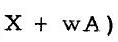
\includegraphics[max width=\textwidth]{2022_07_16_f4e476ee2159dc67e746g-77}

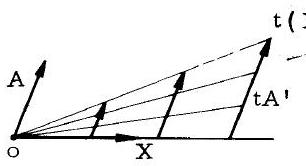
\includegraphics[max width=\textwidth]{2022_07_16_f4e476ee2159dc67e746g-77(1)}

In $\mathrm{M}_{\mathrm{m}}$ :

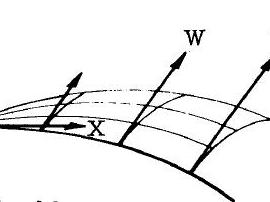
\includegraphics[max width=\textwidth]{2022_07_16_f4e476ee2159dc67e746g-77(2)}

In M:

Fig. 10.1 Jacobi Field

A point $X$ in $M_{m}$ is a conjugate point if exp $p_{m}$ is $\operatorname{singular}$ at $X .$ The point $(m, X)$ in $T(M)$ is called a conjugate point if $X$ is a conjugate point in $M_{\mathrm{m}} .$ A point $m$ in $M$ is conjugate to a point $p$ in $M$ along a geodesic $g$ if there is a conjugate point $X$ in $M_{m}$ such that $\exp _{m} X=p$ and $g$ is a reparameterization of the geodesic $g_{X}(t)=$ $\exp _{m} t X$

Notice there is alorays a neighborhood of zero in $M_{m}$ that is free of conjugate points since $\left(e x p_{m}\right)_{*}$ is non-singular at zero (section 9.3, Cor. 1). For a trivial (and too special) example of conjugate points, let $M$ be the unit sphere about the origin in $R^{3}$. Then the south pole is conjugate to the north pole al ong any geodesic (great circle); moreover, the north pole is conjugate to itself along any geodesic. To see this let $p$ be the north pole, then exp is completely singular on circles about zero in $M_{p}$ which have radius $k \pi$ for integral

THEOREM 4. A point $X$ in $M_{m}$ is a conjugate point iff there is a non-trivial Jacobi field along $g_{X}$ that vanishes at $m$ and $\exp _{m} X$. Proof. If exp $\operatorname{ex}_{m}$ is singular at $X$ let $A^{\prime} \neq 0$ be a vector such that $\left(\exp _{m}\right)_{*} A^{\prime}=0$. Then, letting $A^{\prime}$ denote the associated constant vector field on $M_{m}$, the field $\left(\exp _{m}\right)_{*} t A^{\prime}$ is a non-trivial Jacobi field along $g_{x}$ that vanishes at $m(t=0)$ and $\exp _{m} X(t=1)$

Conversely, let $Z$ be a non-trivial Jacobi field along $g_{X}$ with $Z(0)=Z(1)=0 . \quad$ Let $A=D_{x} Z$ in $M_{m}$ and let $A^{\prime}$ be the associated constant field on $M_{m} \cdot$ Let $Z^{\prime}=\left(\exp _{m}\right)_{*}\left(t A^{\prime}\right)$. Then $D_{X^{\prime}} Z^{\prime}=$ $D_{X}\left[t\left(\exp _{m}\right)_{*} A^{t}\right]=\left(\exp _{m}\right)_{*} A^{\prime}+t D_{X}\left[\left(\exp _{m}\right)_{*} A^{\prime}\right]$, and at $t=0, D_{X} Z^{\prime}=A^{\prime}$ since at zero $\left.(\exp )_{m}\right)_{*} A_{0}^{\prime}=A$. Thus by uniqueness (Theorem 2) $Z=Z^{\prime}$, and hence $Z^{\prime}(1)=\left(\exp _{m}\right)_{*} A_{X}^{\prime}=0$. Since $Z$ is non-trivial $A^{\prime} \neq 0$ and thus $\exp _{m}$ is singular at $X_{.} / /$

Corollary. A point $m$ is conjugate to a point $p$ along a geodesic $g$ iff $p$ is conjugate to $m$ along $g$.

THEOREM 5. Let $g$ be a geodesic whose parameter domain includes $[b, c]$ and suppose $g(b)$ is not conjugate to $g(c)$ along $g$. Then there is a unique Jacobi field $Z$ along $g$ with prescribed values at $g(b)$ and $g(c)$

Proof. Suppose $Z(b)$ and $Z(c)$ are given. By hypothesis, the map $\exp _{G(b)}$ is non-singular at the point $X$ in $M_{G(b)}$ where exp th $_{g(b)} X=g(c)$, i.e., $g(t)=\exp _{g(b)}\left(\frac{t-b}{c-b}\right) X$; hence there is a unique vector $A^{\prime}$ such that $\left(\exp { }_{g(b)^{\prime}}^{)_{*}} A^{\prime}=Z(c)\right.$. Let $Z_{1}=\left(\exp _{g(b)}\right)_{*}\left(t A^{\prime}\right)$ along exp $t X$ (which is along $g$ ). Similarly, we get a unique vector $B^{\prime}$ tangent to $M_{g(c)}$ such that $\left(\exp _{g(c)}\right)_{*} B^{\prime}=Z(b) . \quad$ Let $Z_{2}=\left(\exp _{B(c)}\right)_{*}\left(t B^{\prime}\right)$ along $\exp _{g(c)} t Y$ where exp $g(c) Y=g(b)_{g}$. Then $Z=Z_{1}+Z_{2}$ is a Jacobi field along $g$ with the required values at $g(b)$ and $g(c) .$ Furthermore $Z$ is unique, for if $W$ where another such field, then $Z-W$ would be a Jacobi field that vanishes at $g(b)$ and $g(c)$ and hence must be trivial, so $Z=W . /$

Section 10.2. First and second variation formulae.

Throughout this section let $M$ be a $C^{\infty}$ Riemannian $n$-manifold which is Hausdorff, and let $D$ be the Riemannian connexion. For an alternate approach to the material of this section see Ambrose. ${ }^{3}$

THEOREM.6. Let f be a one-parameter family of geodesics in $M$ which are parameterized by arc length. Then $\langle W \quad T>$ is constant along

\section{each geodesic.}
Proof. The function $\langle T, T\rangle=1$ on the domain of $f$; hence, $0=$

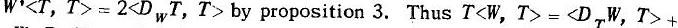
\includegraphics[max width=\textwidth]{2022_07_16_f4e476ee2159dc67e746g-78}\\
$\left\langle W, D_{T} T\right\rangle=\left\langle D_{W} T, T\right\rangle=0$, since $D_{T} T=0 . / /$

Corollary ("perpendicular lemma"). Let $X$ be a unit vector in $M_{m}$. Let $A$ be in $M_{m}$ with $\langle A, X\rangle=0$ and let $A^{\prime}$ be the associated constant vector field on $M_{m}$. Then $\left(\exp { }_{m}\right)_{*} A^{\prime}$ is perpendicular to the geodesic $g_{X}$ at all points where $g_{X}$ defined.

Proof. We may assume $A$ is a unit vector and then define $f(t, w)=$ $\exp _{m} t[(\cos w) X+(\sin w) A]$ for $t$ in the domain of $g_{X}$ and $w$ in an interval about zero. Then $f$ is a one-parameter family of geodesics which are parameterized by arc length. Applying the above theorem, we have $\langle W, T>$ constant along each geodesic. In this case, $W=$

$\left(\exp p_{m}\right)_{*} t[-(\sin w) X+(\cos w) A]$ and $w=0$ along $g_{x} ;$ hence, $<\left(\exp _{m}\right)_{*} t A_{*}$ $T>=t<\left(\exp _{m}\right)_{*} A, T>$ is constant along $g_{X}$. This vanishes at $t=0$, so $\left\langle\left(\exp _{m}\right)_{*} A, T\right\rangle=0$ along $g_{X^{*}} / /$

Let $f$ be a one-parameter family of curves with domain $Q$ and assume $Q$ contains the set $(t, 0)$ for $0 \leq t \leq b$. Let $f_{w}(t)=f(t, w)$ for $(t, w)$ in $Q$, and let $L(w)$ be the length of the curve $f_{w}$ on $[0, b]$, i.e., $L(w)=$ $\int_{0}^{b} \sqrt{\langle T, T} d t$. We define the first and second variations of $L$ in the direction $f$ to be the numbers $L^{\prime}(0)$ and $L^{\prime \prime}(0)$, respectively, where $L^{\prime}=d L / d w .$ Actually, we should call $L^{\prime}(0)$ the "first derivative of $L$ in the direction of the variation $f$ evaluated at $f$, on $[0, b], "$ and a similar statement should be made for the "second variation." Hence. forth we refer to $f_{0}$ as the base curve.

THEOREM 7. In terms of the notation just developed.
$$
L^{\prime}(0)=\langle W, T\rangle \mid \begin{aligned}
&(b, 0) \\
&(0,0)
\end{aligned}-\int_{0}^{b}\left\langle W, D_{T} T\right\rangle_{W=0} d t
$$
when $f_{0}$ is parameterized by arc length. Thus if $f_{0}$ is a geodesic, then $L^{\prime}(0)=\langle W, T\rangle \mid \begin{array}{ll}(b, 0) \\ (0,0)^{\bullet}\end{array}$

\section{Proof. We compute,}
$$
L^{\prime}(w)=\int_{0}^{b}(\partial / \partial w) \sqrt{<T, T>} d t=\int_{0}^{b}<T, T>-(1 / 2)<D{ }_{w} T, T>d t .
$$
When $w=0,\langle T, T\rangle=1$ and
$$
\left\langle D_{W} T, T\right\rangle=\left\langle D_{T} W, T\right\rangle=\frac{d}{d t}\langle W, T\rangle-\left\langle W, D_{T} T\right\rangle
$$
which we integrate to obtain the above formula.//

Notice that theorem 7 shows $L^{\prime}(0)$ only depends on the vector field $W$ along the base curve $f_{0}$ and we may use the general formula of theorem 7 to define the first variation of $L$ in the direction of the field $W$ where $W$ is any $C^{\infty}$ field on the base curve. For each such $C^{\infty}$ field $W$ on a base curve $\sigma$ we can define a one-parameter family $f$ such that $W=f_{*}(\partial / \partial w)$ by letting $f(t, w)=\exp _{\sigma(t)}\left(w W_{\sigma(t)}\right)$.

A curve $\sigma$ between points $p$ and $q$ in $M$ is called an extremal to the fixed end-point problem if $L^{\prime}(0)=0$ for every one-parameter family of curves $f$ such that $f_{0}=\sigma$ on $[0, b]$ and $f(0, w)=p$, while $f(b, w)=q$ for $w$ near $0 .$

THEOREM 8. $A$ curve $\sigma$ between points $p$ and $q$ in $M$ is an extremal iff it is a geodesic.

Proof. If $\sigma$ is a geodesic and the end-points are fixed so $W=0$ at $p$ and $q$, then $L^{\prime}(0)=0$ by theorem 7 .

Conversely, if $L^{\prime}(0)=0$ and $W=0$ at $p$ and $q$, then $\int_{0}^{b}<W, D_{T} T>d t=0$ for all $W$ belonging to admissable (fixed end-point) one-parameter vari ations $f$ of $\sigma .$ If at some point $m$ on $\sigma$ between $p$ and $q$ we suppose $\left(D_{T} T\right)_{m} \neq 0$, then let $W=h D_{T} T$ where $h$ is a $C^{\infty}$ "bump" function such that $h(m)=1, h \geq 0$, and $h=0$ outside a neighborhood of $\dot{m}$ on which $D_{T} T$ doesn't vanish. By the remarks after theorem 7 , there is a oneparameter family $f$ belonging to $W .$ In this case $\left\langle W, D_{T} T>=\left\langle D_{T} T\right.\right.$, $D_{T} T>\geq 0$ is a non-negative function which is non-zero on a neighborhood of $t^{\prime}$ where $o\left(t^{\prime}\right)=m$, hence $\int_{0}^{b}\left\langle W, D_{T} T>d t>0\right.$, which is a con-

tradiction. Thus $D_{T} T=0$, and $\sigma$ is a geodesic. $/ /$ THEOREM 9. For a point $m$ in $M$, let $t>0$ be chosen so $\exp _{m}$

If $W$ a Jacobi field and $<W, T>$ is constant along g, then maps the set $\hat{B}=\left[X\right.$ in $\left.M_{m}:|X|<r\right]$ diffeomorphically onto its image
$$
L^{\prime \prime}(0)=W<T, W>\left.\right|_{(b, 0)^{\circ}} ^{(b, 0)}
$$
Proof. First compute $\left.(\partial / \partial w) \sqrt{\langle T, T\rangle}=\langle T, T\rangle^{-1 / 2<D}, T, T\right\rangle$. Then $\left.\left(\partial^{2} / \partial w^{2}\right) \sqrt{\langle T}, T\right\rangle=-\langle T, T\rangle^{-3 / 2}\left\langle D_{W} T, T>^{2}+\langle T . T\rangle^{-1 / 2}\left(\left\langle D_{W} D_{W} T, T\right\rangle\right.\right.$ $\left\langle D_{W} T, D_{W} T>\right)$. Evaluating on $w=0$, we use $<T, T>=1, D_{T} T=0$, and $D_{T} W=D_{W} T$, to obtain $\left(\partial^{2} / \partial W^{2}\right) \sqrt{ }\langle T, T\rangle=\left\langle D_{W} D_{T}, T>+<D_{T} W\right.$, $D_{T} W>-\left\langle D_{T} W, T>^{2}=\left\langle R(W, T) W+D_{T} D_{W} W, T>+<D_{T} W, D_{T} W>-\right.\right.$ $(T<W, T>)^{2}=T<D_{W} W, T>+<R(W, T) W, T>+<D_{T} W, D_{T} W>-(T<W, T>)^{2}$, which gives the first formula for $L^{\text {" }}(0)$ by integrating.

If $\langle W, T\rangle$ is constant along $g$, then $T<W, T\rangle=0$ which gives the second formula.

If $W$ is Jacobi, then

$\left\langle R(W, T) W, T>=\left\langle R(T, W) T, W>=\left\langle D_{T}^{2} W, W>=T<D_{T} W, W>-<D_{T} W\right.\right.\right.$
$$
D_{T} W>.
$$
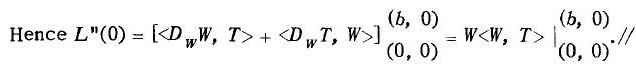
\includegraphics[max width=\textwidth]{2022_07_16_f4e476ee2159dc67e746g-79}

Notice that the first term is the only term in the above formulae that depends on something more than the vector field $W$ along $g$.

Corollary. If $W$ vanishes at the end-points of $g$, then the second variation of $L$ depends only on the field $W$ along $g$. For any vector field $W$ along $g$, let $f_{W}(t, W)=\exp _{\theta(t)} W W$ be the natural one-parameter family associated with $W$, and then $D_{W} W=0$, since the Wavarying curves are geodesics. Letting $L_{W}^{\prime \prime}(0)$ denote the second variation of $L$ in the direction $f_{W}$, then
$$
L_{W}^{\prime \prime}(0)=\int_{0}^{b}\left[<R(W, T) W, T>+<D_{T} W, D_{T} W>-\left(T<W, T>^{2}\right] d t\right.
$$
We next prove two lemmas which are used to prove that geodesics are not minimizing-distance curves past a first conjugate point, and later, to prove conjugate points are isolated along a geodesic in the Riemannian case. B. Then $B$ is the metric ball $B(m, r)=[p$ in $M: d(m, p)<r]$. Furthermore, if $X$ in $B$ and $p=\exp _{m} X$ then $d(m, p)=|X|$, and the geodesic $g_{X}(t)=\exp _{m} t X$ defined on $[0,1]$, realizes the absolute minimum possible curve-length from $m$ to $p$.

Proof. If $T$ is the tangent to $g_{X}$, then $\langle T, T\rangle$ is constant on $g_{X}$ so $\left|g_{X}\right|_{0}^{1}=|X|$. We must show any other broken $C^{\infty}$ curve $\sigma$ from $m$ to $p$ has a length which is greater than or equal to $|X|$, and the theorem will follow.

First suppose $\sigma$ is defined on $[0, b]$ and $\sigma(t)$ is in $B$ for all $t$ in $[0, b]$. Furthermore, suppose $\sigma$ never returns to $m$ after $t=0$, or we could obviously obtain a shorter curve from $m$ to $p$. Let exp $=\exp _{m}$ and let exp ${ }^{-1}$ be the inverse map of $\left.\exp \right|_{B} \cdot \operatorname{Let} f(t)=\left|\exp ^{-1} \sigma(t)\right|^{m}$ for $t$ in $[0, b]$, which defines a broken $C^{\infty}$ function $f$. Let $\vec{o}(t)=$ $\exp ^{-1} \sigma(t), \bar{\gamma}(t)=f(t) X /|X|$, and $\gamma(t)=\exp \bar{\gamma}(t)$. Thus $\gamma$ is a reparameterization of $g_{X}$ which has the same "radial velocity" as $\sigma$. Decompose the tangent to $\bar{\sigma}$ into a radial component $A$ and a vector $V$ which is orthogonal to $A$, thus $T_{\tilde{\sigma}}=A+V$ on $[0, b]$, (actually, $A(t)=$ $f^{\prime}(t) \bar{\sigma}(t) / f(t)$ for $\left.t>0\right)$. Using the perpendicular lemma proved above, we know $\exp _{*} A$ is perpendicular to $\exp _{*} V$, so $\left|T_{\sigma}\right|=\left|\exp _{*} A+\exp _{*} V\right| \geq$ $\left|\exp { }_{*} A\right|=\left|T_{\gamma}\right| \cdot$ Hence, $|\sigma|_{0}^{b} \geq \mid \gamma_{0^{*}}^{b}$ Since $\gamma$ is a reparameterization of $g_{X}$, we have $|\gamma|_{0}^{b} \geq\left|g_{X}\right|_{0}^{1}=|X|$, where the inequality is strict if $f$ is not an increasing function. Thus, $|\sigma|_{0}^{b} \geq|X|$.

If $\sigma(t)$ not in $B$ for all $t$, then $|\sigma|>r>|X|$ by the above paragraph. Hence, $|X|=d(m, p)$ for $X$ in $\hat{B}$, and the geodesic $g_{X}$ realizes this minimum.//

THEOREM 10. Let $f$ be a one-parameter family of curves such that the base curve is a geodesic g parameterized by arc length on the interval $[0, b]$. Then $L^{\prime \prime}(0)=$

$\left\langle D_{W} W, T>\left\{_{(0,0)}^{(b, 0)}+\int_{0}^{b}\left[\left\langle R(W, T) W, T>+<D_{T} W, D_{T} W>-(T<W, T>)^{2}\right] d t\right.\right.\right.$ If $\langle W, T>$ is constant along $f$, then

$L^{\prime \prime}(0)=\left\langle D_{W} W, T>\left.\right|_{(0,0)} ^{(b, 0)}+\int_{0}^{b}\left[<R(W, T) W, T>+<D_{T} W, D_{T} W>\right] d t\right.$ LEMMA 1 (Lagrange identity). If $X$ and $Y$ are Jacobi fields along a geodesic $g$ with tangent field $T$, then $\left\langle D_{T} X, Y\right\rangle-\left\langle X, D_{T} Y\right\rangle$ is constant along g.

Proof. We compute $T\left(\left\langle D_{T} X, Y\right\rangle-\left\langle X, D_{T} Y\right\rangle\right)=\left\langle D_{T}^{2} X, Y\right\rangle-$ $\left\langle X, D_{T}^{2} Y\right\rangle=\langle R(T, X) T, Y\rangle-\langle R(T, Y) T, X\rangle=0$ by the symmetry of the Riemann-Christoffel curvature tensor.//

LEMMA 2. Let $W$ be a continuous piecewise $C^{\infty}$ field along the geodesic $g$ which is parameterized on $[0, b]$, and let $W(0)=0$. If there is no point $g(t)$ that is conjugate to $g(0)$ for $t$ in $[0, b]$, then

$\int_{0}^{b}\left[\langle R(W, T) W, T\rangle+\left\langle D_{T} W, D_{T} W\right\rangle\right] d t>\int_{0}^{b}\left[\langle R(Z, T) Z, T\rangle+\left\langle D_{T} Z, D_{T} Z\right\rangle\right] d$

unless $W=Z$, where $Z$ is the unique Jacobi field along $g$ such that $Z(0)=0$ and $Z(b)=W(b)$

Proof. The field $Z$ is well-defined by theorem $5 .$ Let $Z_{1}, \ldots, Z_{n}$ be a base of $M g(b)$, and extend these vectors by theorem 5 to be Jacobi fields along $g$ that vanish at $g(0)$. Since there is no point $g(t)$ conjugate to $g(0)$, the fields $Z$,..., $Z$ are a base of $M$ for all $t$ in $(0, b]$. Using theorem 3 , write each $Z_{i}=t A_{i}$ where $A_{1}, \ldots, A_{n}$ are $C^{\infty}$ fields that are independent on $[0, b]$. Setting $W=\sum_{i=1}^{n} \oint_{i} A_{i}$, we define continuous piece wise $C^{\infty}$ functions $g_{i}$ on $[0, b]$. Since $g_{i}(0)=0$ we may write $g_{j}=t f$ and thus define continuous piece wise $C^{\infty}$ functions $f_{i}$ on $[0, b]$ such that $W=\sum f_{i} Z_{i \cdot}$ Then $Z=\sum f_{i}(b) Z_{i^{*}}$

Let $D_{T} W=A+B$ where $A=\Sigma\left(T f_{i}\right) Z_{i}$ and $B=\sum f_{i} D_{T^{*}} Z_{\text {Then }}$ The $\left\langle D_{T} W, D_{T} W\right\rangle=\langle A, A\rangle+2\langle A, B\rangle+\langle B, B\rangle$, and

$<R(T, W) T, W>=\Sigma f_{i}<R\left(T, Z_{i}\right) T, W>=\Sigma f_{i}<D_{T}^{2} Z_{i}, W>$
$$
=\sum f_{i}\left[T<D_{T} Z_{i}, W>-<D_{T} Z_{i}, D_{T} W>\right]
$$
$$
\begin{aligned}
& =T\left\langle B, W>-\Sigma\left(T f_{i}\right)\left\langle D_{T} Z_{i}, W>-\langle B, A\rangle-\langle B, B>\right.\right.
\end{aligned}
$$
Hence, $\langle R(T, W) T, W\rangle+\left\langle D{ }_{T} W, D_{T} W\right\rangle=T\langle B, W\rangle+\langle A, A\rangle+\langle A, B\rangle-$ $\sum\left(T f_{i}\right)<D_{T}, Z_{i}>_{0}$ But $\langle A, B\rangle-\Sigma\left(T f_{i}\right)\left\langle D_{T} Z_{i}, W\right\rangle=\Sigma\left(T f_{i}\right) f_{j}\left[<Z_{i} D_{T} Z_{j}>-\left\langle D_{T} Z_{i}, Z_{j}>\right]=0\right.$ by the Lagrange identity, since $Z_{k}(0)=0$ for all $k$. Thus $\int_{0}^{b}[<R(W, T) W$, $\left.T\rangle+\left\langle D_{T} W, D_{T} W\right\rangle\right] d t=\left\langle B_{b}, W_{b}\right\rangle+\int_{0}^{b}\langle A, A\rangle d t$ since $W$ is continuous and $W_{0}=0 .$ Furthermore, $\left\langle B_{b}, W_{b}>=\left\langle f_{i}(b)\left(D_{T} Z_{i}\right)_{b},_{b} W_{b}>=\left\langle\left(D_{T} Z\right)_{b}\right.\right.\right.$ $\left.Z_{b}\right\rangle=\int_{0}^{b}\left[\langle R(Z, T) Z, T\rangle+\left\langle D_{T} Z, D_{T} Z\right\rangle\right] d t . \quad$ Since $\int_{0}^{b}\langle A, A\rangle d t \geq 0$, the inequality in the conclusion follows unless $A \equiv 0$, which implies $f_{i}$ are constant so $W \equiv Z . / /$

THEOREM 11. The arc length on a geodesic $g$ does not equal the distance in $M$ beyond the first conjugate point; i. e., if $g(b)$ is the first point of $g$ that is conjugate to $g(0)$, and $g$ is parameterized by arc length, then the distance $d(g(0), g(a))<a$ for $a>b$.

Proof. Let $Z$ be a non-trivial Jacobi field along $g$ which vanishes at 0 and $b$. Then $\langle Z, T\rangle=0$ by theorem 6 and $L_{z}^{\prime \prime}(0)=0$ by theorem 10 where $L^{\prime}$ is computed from the natrual one-parameter family of curves associated with $Z$. By theorem 9 we obtain $r>0$, so that the neighborhood $B(\xi(b), r)$ is the diffeomorphic image of the r-ball about zero in $M$. Choose numbers $a$ and $c$ such that $0<c<b<a$ and $\sigma(t)$ is in $B(g(b), r)$ for all $t$ in $[c, a]$. Thus the interval $[c, a]$ has no pair of points that are conjugate to each other on $g$. Let $Y$ be the unique Jacobi field along $g$ with $Y(c)=Z(c)$ and $Y(a)=0$. Let $X$ be the field on $[0, a]$ such that $X(t)=Z(t)$ for $t$ in $[0, c]$ and $X(t)=Y(t)$ for $t$ in $[c, a]$. Let $W$ be the field on $[0, a]$ such that $W(t)=Z(t)$ for $t$ in $[0, b]$ and $W(t)=0$ for $t$ in $[b, a]$ (see Fig. 10.2).

Then $\left.L_{W}^{n}\right|_{0} ^{a}=\left.L_{Z}^{n}\right|_{0} ^{b}+\left.L_{W}^{n}\right|_{b} ^{a}=0$ while $\left.L_{X}^{n}\right|_{0} ^{a}=\left.L_{w}^{n}\right|_{0} ^{c}+\left.L_{Y}^{n}\right|_{c^{a}} ^{a} \quad B y$ Lemma 2, we have $\left.L_{W}^{n}\right|_{c} ^{a}>\left.L_{Y}^{n}\right|_{c} ^{a}$, which implies $\left.L_{X}^{n}\right|_{0} ^{a}<\left.L_{W}^{n}\right|_{0} ^{a}=0 .$ Hence there are broken $C^{\infty}$ curves in the natural one-parameter family associated with $X$ whose length from $g(0)$ to $g(a)$ is less that a.//

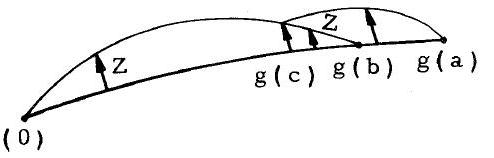
\includegraphics[max width=\textwidth]{2022_07_16_f4e476ee2159dc67e746g-80}

Fig. 10.2 Fields Along a Geodesic Actually, the arc length on a geodesic may cease to measure distance in $M$ long before a conjugate point is reached (think of a right circular cylinder). The conjugate point is where the geodesic ceases to be a minimum-length curve among nearby curves.

THEOREM 12. The conjugate points of a fixed point on a geodesic occur at isolated values of the parameter.

Proof. Let $g(b)$ be any point conjugate to $g(0)$ along the geodesic $g$ (notice it is possible that $g(b)=g(0)$ ). Let $A_{1}, \ldots, A_{t}$ be a base for the kernel of $\left(\exp _{g(0)}\right)_{*}$ at $b T_{0}$ in $M_{G(0)}$, where $T_{t}$ is the tangent to $g$ at $g(t)$, and we assume $\langle T, T\rangle=1$. Choose $A_{r+1}, \ldots, A_{n}$ so $A_{1}, \ldots$ $A_{n}$ are independent and let $Z_{i}(t)=\left(\exp { }_{\varepsilon(0)}\right)_{*} t A_{i}^{*}$ Then the fields $Z_{1}, \ldots, Z_{n}$ are Jacobi fields along $g$ that vanish at 0 and are indepen dent for all values of $t$ except 0 and conjugate values. We show there exists an $\epsilon>0$ such that $Z \ldots, Z$ are independent for $0<|t-b|<\epsilon .$ This is done by showing $D_{T} Z_{1}, \ldots, D_{T} Z, Z$ are independent at $b$ and then $Z,(t-b), \ldots, Z /(t-b), Z{ }_{t} /{ }^{t}+\ldots, Z$ are independent for $0<|t-b|<\epsilon_{0}$

Since $A_{t+1} \ldots, A_{n}$ are independent at $b T_{0}$, we know $Z_{r+1}, \ldots, Z_{n}$ are independent at $b .$ For $i \leq r,\left(D_{T} Z_{i}\right)_{b} \neq 0, \operatorname{since}\left(Z_{i}\right)_{b}=0$ and $Z_{i}$ is non-trivial. If $\sum_{i=1}^{r} c_{i}\left(D_{T_{i}}^{Z_{i}}\right)_{b}=0$, let $W=\sum_{1}^{t} c_{i} Z_{i^{*}}$ Then $W$ is a Jacobi field with $W_{b}=0$ and $\left(D_{T} W\right)_{b}=0$; hence $W \equiv 0$. For small $a>0$, we know $Z_{1}, \ldots, Z_{r}$ are independent, and $\Sigma_{1}^{r} c_{i}\left(Z_{i}\right)_{a}=0$ implies $\mathrm{c}_{i}=0$ for all $i_{.}$Thus $D_{T} Z_{1}, \ldots, D_{T} Z_{\text {r }}$ are independent at $b .$ We now show for $i \leq r$ and $j>r, D_{T_{i}}^{Z_{i}}$ is orthogonal to $Z_{j}$ at $b$. By the Lagrange identity $\left\langle D_{T} Z_{i}, Z_{i}\right\rangle-\left\langle Z_{i}, D_{T} Z_{j}\right\rangle$ is constant along $g$. Since $Z_{i}$ and $Z_{j}$ vanish at 0 , and $Z_{i}$ vanishes at $b$, we have $\angle D_{T} Z_{i}$ $Z_{j}>=0$ at $b_{.}$Thus $D_{T} Z_{1} \ldots, D_{T} Z_{,}, Z_{s+1}, \ldots, Z_{n}$ are independent at $b$ and hence in some neighborhood of $b^{r}$. Since $Z_{i}(t) /(t-b) \rightarrow$ $\left(D_{T} Z_{i}\right)_{b}$ as $t \rightarrow b$, the conclusion follows.//

Section 10.3. Geometric interpretation of Riemannian curvature.

In this section, let $M$ be a Riemannian manifold, $g$ be a geodesic in $M$ with unit tangent $T, A_{0}$ be a unit vector in $M_{g(0)}$ which is orthogonal to $T_{0}, A^{\prime}$ be the constant vector field on $M_{g(0)}$ generated by $A_{0}, \exp =\exp _{g(0)}, A=\exp _{*} A^{\prime}$, and where $A_{t} \neq 0$ let $K=\langle R(T, A) A, T$ $/\langle A, A\rangle$ as a function of $t$ al ong $g$. We study the relationship be- tween the Riemannian curvature $K(t)$ of the plane section spanned by $A_{t}$ and $T_{t}$ and the length of the vector $A_{t:}$ The field $t A$ is used in the computation since it is a Jacobi field.

LEMMA. If $t A_{t} \neq 0$, then

(1) $T|t A|=\left\langle D_{T} t A, t A>/|t A|=|A|+t<D_{T} A, A>/|A|\right.$,

(2) $T^{2}|t A|=-|t A| K(t)+H(t)$ where $H(t) \geq 0$, and

(3) $\left|A_{t}\right|=1-K(0)\left(t^{2} / 6\right)+G(t) t^{3}$ for $t$ in a neighbothood of zero where $G$ is $C^{\infty}$

Proof. We compute $T|t A| \Rightarrow T \sqrt{\langle t A, t A\rangle}=\left\langle D_{T} t A, t A\right\rangle /|t A|=$ $\left\langle A+t D_{T} A, t A>/|t A|=|A|+t<D_{T} A, A>/|A| \cdot\right.$ Thus
$$
\begin{aligned}
&T^{2}|t A|=\left[\left\langleD_{T}^{2} t A, t A>+\left\langle D_{T} t A_{T} D_{T} t A>-\left\langle D_{T} t A, t A>^{2} /\langle t A, t A>] /|t|\right.\right.\right.\right. \\
&\quad=\left[\left\langleR(T, t A) T, t A>|t A|^{2}+\left|D_{T} t A\right|^{2}|t A|^{2}-\left\langle D_{T} t A, t A>^{2}\right] /|t A|^{3}\right.\right. \\
&\quad=-|t A| K(t)+H(t)
\end{aligned}
$$
where $H(t)=\left[\left|D_{T} t A\right|^{2}|t A|^{2}-<D_{T} t A, t A>^{2}\right] /|t A|^{3} .$ The Schwartz inequality implies $H(t) \geq 0$. A straightforward computation shows as $t \rightarrow 0, H(t) \rightarrow 0$, and $H^{\prime}(t) \rightarrow 0, \operatorname{since}\left(D_{T} A\right)_{0}=0$ (use normal coord.). Hence as $t \rightarrow 0$, we have $|t A| \rightarrow 0, T|t A| \rightarrow\left|A_{0}\right|=1, T^{2}|t A| \rightarrow 0$, and $T^{3}|t A| \rightarrow-K(0)$

Since $A_{t}$ does not vanish near $t=0$, the function $\left|A_{t}\right|$ is $C^{\infty}$ at 0 , and hence $F(t)=\left|t A_{t}\right|$ admits a representation
$$
F(t)=F(0)+F^{\prime}(0) t+F^{\prime \prime}(0) t^{2} / 2+F^{\prime \prime}(0) t^{3} / 6+G(t) t^{4}
$$
for $t$ in a neighborhood of 0 where $G$ is a $C^{\infty}$ function on this neighborhood. Substituting the values for the derivatives of $F$ and cancelling a factor $t$ then gives (3).//

The following theorem derives its form essentially from some class notes of Ambrose. THEOREM 13. If $K(t) \leq 0$ for $t$ in $[0, b]$, then $\left|A_{t}\right| \geq\left|A_{0}\right|=1$ for $t$ in $[0, b] .$ Thus if $K \leq 0$ for all plane sections at all points of $M$, then $M$ has no conjugate points. If $K(0)<0$, then $\left|A_{t}\right| \geq 1$ for $t$ near zero, and if $K(0)>0$, then $\left|A_{t}\right| \leq 1$ for $t$ near zero.

Proof. Let $F(t)=\left|t A_{t}\right|-t\left|A_{0}\right|=\left|t A_{t}\right|-t$. Then $F(0)=0, F^{\prime}(0)=0$, and $F^{\prime \prime}(t)=T^{2} \mid t A t \geq 0$ if $K(t) \leq 0$. Applying the Mean Value Theorem twice, $F(t)=F^{\prime}(\bar{t}) t=F^{\prime \prime}(\bar{t}) \bar{t} t \geq 0$ where $0 \leq \bar{t} \leq \bar{t} \leq t \leq b$. Hence $A_{t} \mid \geq 1$ for $t$ in $[0, b]$.

The second sentence of the theorem follows from the first, and the last two sentences follow from (3) in the lemma.//

We obtain a geometric interpretation of Riemannian curvature from the following considerations (see Fig. 10.3). The vector $A^{\prime}$ at the point $b T_{0}$ in $M_{g(0)}$ is tangent to the circle $\sigma$ of radius $b$ about the origin which lies in the plane of $A_{0}$ and $T_{0} .$ Hence $A=\exp _{*} A^{\prime}$ is the tangent at $\exp \left(b T_{0}\right)$ to the curve $\exp \circ \sigma$ in $M$. If $b$ is sufficiently small, then exp o $\sigma$ passes through points that are exactly $b$ units distant from $g(0)$. If $\left|A_{b}\right|>\left|A^{\prime}\right|$ then the curve exp o $\sigma$ is "stretchin the curve $\sigma$ near $b T_{0}$ and the geodesics emanating from $g(0)$ that are determined by $\sigma$ are "spreading out." A corresponding statement applies to the case $\left|A_{b}\right|<\left|A^{\prime}\right|$\\

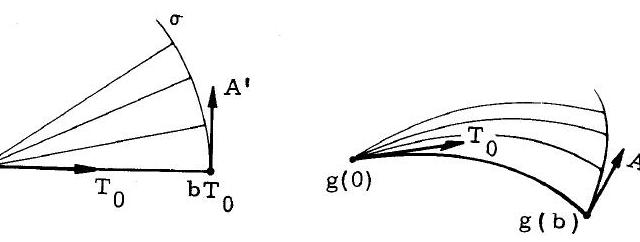
\includegraphics[max width=\textwidth]{2022_07_16_f4e476ee2159dc67e746g-82}

$\operatorname{In} M \operatorname{g}(0)$ In $M$

Fig. 10.3 Comparing Geodesics

\section{Section 10.4. The Morse Index Theorem.}
Our approach to this section is based on the notes of Bott. For further material see Milnor, ${ }^{3}$ Ambrose, ${ }^{2}$ and Morse. Let $M$ be a $C^{\infty}$ manifold and let $f$ be a real valued $C^{\infty}$ function defined on a neighborhood of a point $m$ in $M$. The point $m$ is a critical point of $f$ if $\left(f_{*}\right)_{m}$ is the zero linear transformation on $M_{m^{*}}$ If $m$ is a critical point of $f$, we define a symmetric bilinear function $H: M_{m} \times M_{m} \rightarrow R$ by $H\left(X_{m}, Y_{m}\right)=X_{m}(Y f)$, where $Y$ is any $C^{\infty}$ vector field about $m$ whose value at $m$ is $Y_{m} .$ It is a simple exercise to show $H\left(X_{m}, Y_{m}\right)$ is independent of the field $Y$ and is symmetric and bilinear (see problem 95). The function $H$ is called the Hessian of $f$ at $m$. The index of $H$ is defined to be the dimension of a maximal subspace $V$ of $M$ on which $H$ is negative definite (and $V$ is maximal if it is not properly contained in a subspace $V^{\prime}$ on which $H$ is negative definite). The null space of $H$ is the subspace $V=[X$ in $M: H(X, Y)=0$ for all in $M_{m}$. The nullity of $H$ is the dimension of its null space. We denote the index of $H$ and the nullity of $H$ by $I(f)$ and $N(f)$, respectively, and call them the index of $f$ at $m$ and the nullity of $f$ at $m$ respectively. The positivity $P(f)$ is the integer such that $P(f)$, $I(f)+N\left(f_{m}\right)$ is the dimension of $M$ The index of $H$ intuitively gives the number of dimensions of directions in $M$ in which $f$ is decreasing

Next we need the definition of the conjugate degree of points along a geodesic. Let $\&$ be a geodesic in a manifold with connexion. The conjugate degree of the point $g(t)$ (with respect to $g(0)$ ) is the dimension of the kernel of (exp the point $g(t)$ (with respect to $g(0)$ ) is the dimen to $g$ at $g(0)$ and $g$ is parameterized by arc length. Thus the conjugate degree of the point $g(t)$ is the maximum number of linearly independent Jacobi fields along $g$ that vanish at 0 and $t$.

The Morse Index Theorem relates the concepts just defined. Roughly, it says, for a particular geodesic segment in a Riemannian manifold $M$, the distance function can be used to define a $C^{\infty}$ function $L$ on a manifold $C$, and then the index of $L$ at a particular critical point is equal to the sum of the degrees of conjugate points along the geodesic segment.

For the rest of the section let $M$ be a $C^{\infty}$ Riemannian Hausdorff $n$ manifold. If $m$ in $M$, then a local geodesic submanifold of $M$ at $m$ is a submanifold $C$ defined as follows. Let $B$ be an open ball about the origin (zero) in $M_{m}$ which exp $\mathrm{e}_{m}$ maps diffeomorphically into $M$, and let $V$ be any subspace of $M_{m}$. Then the submanifold $C=\left[\exp _{m} X: X\right.$ in $B \sim V]$ is a local geodesic submanifold of $M$. Note $C$ contains geodesic segments of geodesics emanating from $m$ whose tangent vectors lie in $V$ (see Fig. 10.4).

LEMMA. Let A be a convex neighborhood of $M$, let $p_{1}$ and $p_{2}$ be in $A$, let $g$ be the unique geodesic from $p_{1}$ to $p_{2}$ which lies in $A$ and is parameterized by arc length, let $T$ be the tangent field to $g$, let $C_{1}$ and $\mathrm{C}_{2}$ be disjoint local geodesic hypersurfaces of $A$ through $p$ and $p_{2}$, respectively, that are orthogonal to $T$, and finally, let $C=$ $C_{1} \times C_{2}$ (see Fig. 10.4). If $\left(m_{1}, m_{2}\right)$ is a point of C, let $d\left(m_{1}, m_{2}\right)$ be the distance from $m_{1}$ to $m_{2}$; thus $d$ is real-valued $C^{\infty}$ function from C into $R$ (problem 96). Let $W=\left(W_{1}, W_{2}\right)$ and $U=\left(U_{1}, U_{2}\right)$ be vectors tangent to $C$ at $\left(p_{1}, p_{2}\right)$, where $W_{i}$ and $U_{i}$ are in $M_{p}$ for $i=1,2$, and let $U$ al so denote the unique Jacobi field along $g$ determined by $U$ and $U_{2}$

Then $p=\left(p_{1}, p_{2}\right)$ is a critical point of $d$ on $C$ and
$$
H_{p}(U, W)=U_{p}(W d)=\left[\left\langle W, D_{T} U>-I_{T}(U, W)\right]_{p_{1}}^{p_{2}}\right.
$$
where $I_{T}$ at $p_{i}$ is the second fundamental form of $C_{i}$ with respect to the normal in the direction of $T$.

\includegraphics[max width=\textwidth]{2022_07_16_f4e476ee2159dc67e746g-83}

Fig. 10.4 Cross Manifolds

Proof. A two-parameter family of geodesics is a $C^{\infty}$ function $f$ mapping an open set $Q$ in $R^{3}$ into $M$ such that the curves $f_{\left(u_{0}, w_{0}\right)}(t)=$ $f\left(t, u_{0}, w_{0}\right)$, obtained from $f$ by fixing the coordinates in the last two slots, are geodesics. Let $f$ be such a map and suppose $Q$ contains the set $(t, 0,0)$ for $0 \leq t \leq b$. Call the geodesic $g=f(0,0)$ the base geodesic and assume $g$ is parameterized by arc length. Let $T=$

$f_{*}(\partial / \partial t), U=f_{*}(\partial / \partial u)$, and $W=f_{*}(\partial / \partial w) ;$ then $T, U$, and $W$ are Jacobi fields along the geodesics of $f$, while $D_{T} W=D_{W} T, D_{T} U=D_{U} T$, and $D_{U} W=D_{W} U$ by section 10.1. We assume further that $\langle T, U\rangle$ and

$\langle T, W\rangle$ are constant on $g$; hence $\left\langle D_{T} U, T\right\rangle=0$ and $\left\langle D_{T} W, T\right\rangle=0$ on g. For $(u, w)$ near $(0,0)$, let $L(u, w)=\int_{0}^{b} \sqrt{\langle T, T} d d$. Notice $\langle T, T\rangle$ is a function on $Q$ which depends only on $u$ and $w$ since the $t$-curves

\includegraphics[max width=\textwidth]{2022_07_16_f4e476ee2159dc67e746g-83(1)}\\
$\left(L_{W}\right)_{(0,0)}=\int_{0}^{b}\left\langle D_{T} W, T>d t=0\right.$ since $\left.<T, T\right\rangle=1$ on $g$. Differentiating again,
$$
\begin{gathered}
\left(L_{w u}\right)=\left(\partial^{2} L / \partial u \partial w\right)=\int_{0}^{b}\left[-<T, T>^{-3 / 2<D_{U} T, T><D_{W} T, T>}\right. \\
\left.+<T, T>-1 / 2\left(<D_{U} D_{W} T, T>+<D_{W} T, D_{U} T>\right)\right] d t
\end{gathered}
$$
Evaluating on $g$, we have
$$
\begin{aligned}
&\left(L_{w u}\right)_{(0,0)}=\int_{0}^{b}\left[\left\langle D_{U} D_{T} W, T\right\rangle+\left\langle D_{T} W, D_{T} U\right\rangle\right] d t \\
&\left.\quad=\int_{0}^{b}\left[R(U, T) W+D_{T} D_{U} W, T>+T<W, D_{T} U\right\rangle-\left\langle W, D_{T}^{2} U\right\rangle\right] d t .
\end{aligned}
$$
But, since $U$ is Jacobi,

$\left\langle R(U, T) W, T>-\left\langle W, D \frac{T}{2} U\right\rangle=\langle R(U, T) W, T>-<W, R(T, U) T\rangle=0\right.$

hence,
$$
\left(L_{w u}\right)_{(0,0)}=\int_{0}^{b}\left[<D_{T} D_{U} W, T>+T<W, D_{T} U>\right] d t
$$
$=\int_{0}^{b}\left[T<D_{U} W, T>+T<W, D_{T} U>\right] d t$

$=\left\langle D_{U} W, T>+\left.\left\langle W, D_{T} U\right\rangle\right|_{(0,0,0)} ^{(b, 0,0)}\right.$ We apply the above analysis to prove the lemma. Let $f_{(u, w)}(t)=$ $f(t, u, w)$ be the unique geodesic in $A$ from $\exp _{p_{1}}\left(u U_{1}+w W_{1}\right)=$ $\gamma_{1}(u, w)$ to $\exp _{p_{2}}\left(u U_{2}+w W_{2}\right)=\gamma_{2}(u, w)$ which is parameterized on $[0, b]$. Then $f$ is a two-parameter family of geodesics satisfying the above requirements. Furthermore $d\left(\gamma_{1}(u, w), \gamma_{2}(u, w)\right)=L(u, w)$, hence $H_{p}(U, W)=\left\langle D_{U} W_{i}, T\right\rangle+\left\langle W_{i}, D_{T} U_{i}>\left.\right|_{i} ^{1}=2\right.$. But letting $D^{\prime}$ be the induced Riemannian connexion on $C$, by the Gauss equation we get
$$
D_{U_{i}} W_{i}=D_{U_{i}}^{\prime} W_{i}-I_{T}\left(U_{i}, W_{i}\right) T ;
$$
hence $H_{p}(U, W)=\left[\left\langle W, D_{T} U>-I I_{T}(U, W)\right]_{p_{1}}^{p_{2}} . / /\right.$

THEOREM 14 (Morse Index Theorem). Let $g$ be a geodesic in $M$ which is parameterized by arc length on the interval $[0, b] .$ Let $r>0$ be chosen such that the balls $B(g(t), 2 r)$ are convex neighborhoods of $g(t)$ for $0 \leq t \leq b .$ Let $\bar{m}=\left(m_{1}, \ldots, m_{k}\right)$ be a sequence of points on $g$ such that $m_{i}=g\left(t_{i}\right), 0<t_{i}<t_{i+1}<b$, and

(1) $0<d\left(m_{i}, m_{i+1}\right)<t$

for $i=0, \ldots, k$ where $m_{0}=g(0)$ and $\mathrm{m}_{k+1}=g(b) .$ Let $C_{i}$ be a local geodesic submanifold which is orthogonal to $g$ at $m_{i}$ and contained in $B\left(m_{i}, r\right)$ for $1 \leq i \leq k$, and let $C=C_{1} \times \ldots \times C_{k^{*}} \operatorname{Let} L: C \rightarrow R$ by $L(\bar{p})=\sum_{i=0}^{k} d\left(p_{i}, p_{i+1}\right)$ where $\bar{p}=\left(p_{1}, \ldots, p_{k}\right)$ in $C, p_{0}=g(0)$ and $p_{k+1}=g(b)(\operatorname{see} F i g .10 .5)$

Then $L$ is $C^{\infty}$ on $C, \bar{m}$ is a critical point of $L$, the nullity of $L$ at $\bar{m}$ equals the conjugate degree of $g(b)$ (with respect to $g(0)$ ) and $I\left(L_{\bar{m}}\right)=\sum_{0<t \leq b} \operatorname{deg} g(t)$

\includegraphics[max width=\textwidth]{2022_07_16_f4e476ee2159dc67e746g-84}

Fig. $10.5$ Cross Manifolds

Before proving the theorem we make some remarks. The fact that $N\left(L_{\bar{m}}\right)$ is the conjugate degree of $g(b)$ is often called the Nullity The\begin{CJK}{UTF8}{mj}日\end{CJK}rem. The Index Theorem shows $I\left(L_{\bar{m}}\right)$ and $N\left(L_{\bar{m}}\right)$ are independent of the position of the points $m_{i}$ and the number of points $k$, as long as condition (1) is satisfied.

Proof. Let $L_{i}: C \rightarrow R$ be defined by $L_{i}(\bar{p})=d\left(p_{i}, p_{i+1}\right)$ for $i=$ $0, \ldots, k$. Then $L$ is $C^{\infty}$ since $L=\sum_{i=0}^{k} L_{i}$ and each $L_{i}$ is $C^{\infty}$. By the lemma, the point $\bar{m}$ is a critical point of each $L_{i}$ and hence is a critical point of $L$.

To compute the nullity of $L$ at $\bar{m}$ let $U$ and $W$ be tangent to $C$ at $\vec{m}$ where $U=\left(U_{1} ; \ldots ; U_{k}\right)$ and $W=\left(W_{1} ; \ldots ; W_{k}\right)$ with $U_{i}$ and $W_{i}$ in $M_{m}$ for all $i_{.}$Let $U_{0}=W_{0}$ and $U_{k+1}=W_{k+1}$ be the zero vectors at $g(0)$ and $g(b)$, respectively. By the lemma,

$U_{-\bar{m}}(W L)=\Sigma_{0}^{k} U_{\bar{m}}\left(W L_{i}\right)$

$=\Sigma_{i=1}^{k}\left[\left\langle W_{i+1}, D_{T} U_{i+1}^{-}\right\rangle-I_{T}\left(U_{i+1}, W_{i+1}\right)-\left\langle W_{i}, D_{T} U_{i}^{+}\right\rangle+I_{T}\left(U_{i}, W_{i}\right)\right]$

$=\sum_{i=1}^{k}\left\langle W_{i}, D_{T} U_{i}^{-}-D_{T} U_{i}^{+}\right\rangle$

where $U_{i}^{-}$is the Jacobi field on $\left[t_{i-1}, t_{i}\right]$ agreeing with $U$ at the endpoints, and $U_{i}^{+}=U_{i+1 \cdot}^{-}$If $U$ is in the null space of $H_{L}$ at $\bar{m}$, then $U_{m^{-}}(W L)=0$ for all $W$; hence $D_{T} U_{i}^{-}=D_{T} U_{i}^{+}$for all $i$, which implies $U$ is a Jacobi field along $g$ that vanishes at 0 and $b$. This proves the nullity theorem. We now work on the index of $L$ at $\bar{m}$. Let us refer to a point $(\bar{m}, b)$ in $M^{k} \times R$ which satisfies the conditions stated in the third sentence of the theorem as an admissable partition. Let $N=k(n-1)$, and for each admissable partition $(y, t)$ let $C_{y}$ be the product of $k$ local geodesic submanifolds crossing $g$ at the points of $y, \operatorname{let} L_{(y, t)}: C_{y} \rightarrow R$ be the function corresponding to $L$ in the theorem, and let $F$ map $R^{N}$ into the tangent space to $C_{y}$ at $y$ by $F_{y}\left(a_{i}, \ldots, a_{N}\right)=\left(\sum_{1}^{n-1} a_{i} e_{i}\left(y_{1}\right)\right.$; $\left.\sum_{1}^{n-1} a a_{n-1}+e_{j}\left(_{2}\right), \ldots\right)$, where $e_{1}, \ldots, e_{n-1}, T$ is an orthonormal parallel base field along $g$. Then let $H_{(y, t)}, I_{(y, t)}, P_{(y, t)}$, and $N_{(y, t)}$ denote the Hessian, index, positivity, and nullity respectively, of $H_{L}$ o $F_{y^{*}}$ Thus $H_{(y, t)}$ is a symmetric bilinear form on $R^{N}$ which is continuous in $y$ and $t .$

For each admissable partition $\left(y_{0}, t_{0}\right)$ there is a neighborhood (in $M^{k} \times R$ ) such that
$$
I_{(y, t)} \geq I_{\left(y_{0}, t_{0}\right)} \quad \text { and } \quad P_{(y, t)} \geq P_{\left(y_{0}, t_{0}\right)}
$$
for $(y, t)$ in this neighborhood. This follows since $I_{\left(y_{0}, t_{0}\right)}$ is the dimension of a subspace $V$ of $R^{N}$ such that $H_{\left(y_{0}, t_{0}\right)}\left(W^{\prime}, \phi\right)<0$ for all non-zero $W$ in $V$, and by continuity the inequality must hold on a neighborhood of $\left(y_{0}, t_{0}\right)$. A similar argument handles the positivity case.

Fix y such that $\left(y, b_{1}\right)$ and $\left(y, b_{2}\right)$ are admissable partitions with $b_{1} \leq b_{2} .$ We show

(3) $I_{\left(y, b_{1}\right)} \leq I_{\left(y, b_{2}\right)}$ and $P_{\left(y, b_{1}\right)} \geq P_{\left(y, b_{2}\right)^{\circ}}$

For $x$ in the cross manifold $C_{y}$, let $A(x)=L_{\left(y, b_{2}\right)}(x)$ and $B(x)=$ $L_{\left(y, b_{1}\right)}(x)+d\left(g\left(b_{1}\right), g\left(b_{2}\right)\right)$. Then $A(x) \leq B(x)$ by the triangle inequality and $\boldsymbol{A}(\boldsymbol{y})=\boldsymbol{B}(\mathrm{y})$. On a curve $\gamma(w)$ with tangent $W$ that is tangent to $C_{y}$ at $y=\gamma(0)$, we have
$$
A^{\circ} y(w)=A(y)+H_{\left(y, b_{2}\right)}(W, W)\left(w^{2} / 2\right)+\ldots
$$
while
$$
B \circ \gamma(w)=B(y)+H_{\left(y, b_{1}\right)}(W, W)\left(w^{2} / 2\right)+\ldots
$$
Thus $H_{\left(y, b_{2}\right)}(W, W) \leq H_{(y, b, 1)}(W, W)$ for all $W$, and if $H_{(y, b, 1)}$ is negative definite on a subspace $V$ then so is $H_{\left(y, b_{2}\right)}$, which implies $I_{(y, b, 1)} \leq$ $I_{\left(y, b_{2}\right)}$, and similarly, $P_{\left(y, b_{1}\right)} \geq P_{\left(y, b_{2}\right)}$.

If $g(t)$ is not a conjugate point of $g(0)$, then $H(y, t)$ is non-singular on a neighborhood of $(y, t)$, since the conjugate points are isolated, and hence,

(4) $I_{(y, t)}$ and $P_{(y, t)}$

are constant on a neighborhood of $(y, t)$.

We now use the properties $(2),(3)$, and $(4)$ to compute $I\left(L_{y}\right)$. Let $a_{1}, \ldots, a_{s}$ be the points on $[0, b)$ that are conjugate to 0 . If $0<t<a_{1}$ we know $P_{(y, t)}=N, I_{(y, t)}=0$, and $N_{(y, t)}=0$ by theorem 9 and property (-4). At $t=a_{1}, N_{\left(y, a_{1}\right)}=\operatorname{deg} g\left(a_{1}\right), I_{\left(y_{1} a_{1}\right)}=0$ by (2) since $I_{(y, t)}=0$ for $t<a_{1}$, and hence $P_{\left(y, a_{1}\right)}=N-\operatorname{deg} g\left(a_{1}\right)$. If $a_{1}<t<a_{2}$, and $t$ near $a_{1}, P_{(y, t)} \geq P_{(y, a, 1)}$ by $(2)^{1}$ and $P_{(y, t)} \leq P_{(y, a, 1)}$ by $(3)$, hence $P_{(y, t)}=N-\operatorname{deg} g\left(a_{1}\right), N_{(y, t)}=0$, and $I_{(y, t)}=\operatorname{deg} g\left(a_{1}\right)$. The situation then remains unchanged for $a_{1}<t<a_{2}$ by (4). For $t=a_{2}$, we repeat the above reasoning to compute $N_{\left(\gamma_{0} a_{2}\right)}=\operatorname{deg} g\left(a_{2}\right), I_{\left(y, a_{2}\right)}=\operatorname{deg} g\left(a_{1}\right)$ and $P_{\left(y, a_{2}\right)}=N-\Sigma_{0 \leq t \leq a_{2}}$ deg $g(t)$. Continuing the argument, we ob$\operatorname{tain} I\left(L_{y}\right)^{2}=I_{(y, b)}=\sum_{0<t<{ }_{b}} \operatorname{deg} \delta(t) . / /$

Section 10.5. Completeness.

The theorem that follows gives useful criteria for a Riemannian manifold to be complete. The analytic case was first studied by Hopf-Rinow. The approach we give essentially follows de Rham ${ }^{2}$

THEOREM 15. If $M$ is a connected Hausdorff Riemannian manifold, then (a), (b), (c), and (d), stated below, are equivalent statements, and anyone of them implies (e).

\section{Notes on Differential Geometry}
(a) The exponential map is everywhere defined on $T(M)$.

(b) The manifold is complete with respect to its Riemannian metric.

(c) Bounded closed sets in $M$ are compact.

(d) The closed balls $\bar{B}(m, r)$ are compact for one $m$ in $M$ and all $r>0$

(e) Any two points in $M$ can be joined by a geodesic segment whose length equals the distance between the two points.

Proof. The implications $(\mathrm{d}) \Rightarrow(\mathrm{c}) \Rightarrow(\mathrm{b}) \Rightarrow$ (a) are all simple. We show (a) implies (d) and (e). Let $m$ be a fixed point of $M, 1$ et $B_{t}=B(m, r) S_{t}=\bar{B}(m, r)$, and let $E_{t}=\left[p\right.$ in $S_{t}:$ there is a geodesic

\includegraphics[max width=\textwidth]{2022_07_16_f4e476ee2159dc67e746g-86}\\
and $E_{r}=S_{t}$ for all $r$, which proves $(\mathrm{d})$ and $(\mathrm{e})$.

LEMMA 1. The set $E_{r}$ is compact for all $r$.

Proof. Fix $r$ and let $\left[m_{k}\right]$ be a sequence of points in $E_{r^{\circ}} B_{y}$ (a) there exist points $X_{k}$ in $M_{m}$ such that $\exp _{m} X_{k}=m_{k}$ for all $k_{.}$This follows since a geodesic can always be written as a composite map which is the exponential of a ray in a tangent space. Then $|X|<r$ for all $k$, hence $\left[X_{k}\right]$ is a sequence of points in the compact set $\bar{B}(0, r)$ in the Euclidean space $M$. Thus we obtain a subsequence (which we reindex if necessary) $\left[X_{k}\right]$ that converges to $X$ in $M$ with $|X| \leq r$. The corresponding subsequence $\left[m_{k}\right]$ converges to exp $X$, which lies in $E_{r}$ since $\exp _{m}$ is $C^{\infty}$.

LEMMA 2. If $E_{t}=S_{t}$ for a fixed $r$, and $d(m, p)>t$, then there is a point $\bar{m}$ such that $d(m, \bar{m})=r$ and $d(m, p)=r+d(\bar{m}, p)$.

Proof, For each integer $k>0$, let $\gamma_{k}$ be a broken $C^{\infty}$ curve from $m$ to $p$ with $\left|\gamma_{k}\right|<d(m, p)+(1 / k)$. Let $m_{k}$ be the last point on each $\gamma_{k}$ that lies in $S_{r}$, so $d\left(m, m_{k}\right)=r$. Since $S_{r}$ is compact, the sequence $\left[m_{k}\right]$ has a limit point $\bar{m}$ and $d(m, \bar{m})=r .$ But $d\left(m_{k}, p\right) \leq\left|\gamma_{k}\right|_{m}^{p}=$ $\left|\gamma_{k}\right|_{m}^{p}-\left|\gamma_{k}\right|_{m}^{m} \leq\left|\gamma_{k}\right|-r<d(m, p)+(1 / k)-$ r. Hence $d(\bar{m}, p) \leq$

$d(m, p)-r$, and the triangle inequality proves the opposite inequality. LEMMA 3. $F_{\text {or } r} \geq 0, E_{r}=S_{r^{*}}$

\section{Chap. 10 Topics in Riemannian Geometry}
Proof. The proof uses a continuous induction argument on $r .$ By definition, $E_{r} \subset S_{r}$ for all $r_{*}$ For $f=0, E_{0}=S_{0^{*}}$ If $E_{r}=S_{r}$, then trivial $E_{r^{\prime}}=S_{r^{\prime}}$ for all $r^{\prime}<r$. Conversely, if $E_{r^{\prime}}=S_{r}^{\prime}$ for all $r^{\prime}<r$, then $E_{r}=S_{r^{*}}$ This follows by taking any point $p$ in $S_{r}$ and then choosing $\left[p_{k}\right] \rightarrow p$ such that each $p_{k}$ in some $S_{r^{\prime}}$ for $r^{\prime}<r$. Hence each

$p_{k}$ in $E_{r} t \subset E_{r}$, and $E_{r}$ is compact, which implies the limit $p$ is in $E_{r^{\circ}}$ Finally, if $E_{r}=S_{r}$, then there is an $\epsilon>0$ such that $E_{r+\varepsilon}=S_{r+\varepsilon^{*}}$

Since $S_{r}$ is compact, we obtain a number $2 \epsilon>0$ such that for all $p$ in $S_{t}$ the map exp$p_{p}$ is a diffeo from $\left[X\right.$ in $\left.M_{p}:|X|<2 \epsilon\right]$ on to $B(p, 2 \epsilon)$. Take $p$ in $S_{r+\varepsilon}$. By lemma 2, there is a point $\bar{m}$ with $d(m, \bar{m})=r$ and $d(\bar{m}, p)=d(m, p)-d(m, \bar{m}) \leq r+\epsilon-r \leq \epsilon$. Hence there is a geodesic segment $\gamma_{1}$ from $m$ to $\bar{m}$ with $\left|\gamma_{1}\right|=r$, and a geodesic segment $\gamma_{2}$ from $\bar{m}$ to $p$ with $\left|\gamma_{2}\right|=d(\bar{m}, p)$ Joining $\gamma_{1}$ and $\gamma_{2}$ gives a broken $C^{\infty}$ curve $y$ from $m$ to $p$ with $|\gamma|=d(m, p)$. Parameterizing $\gamma$ by arc length, there can be no breaks in $\gamma$, so $\gamma$ is geodesic. Thus $p$ in $E_{t}+\varepsilon \cdot / /$

We can now prove a classical theorem which illustrates how assumptions about the Riemannian curvature can affect the topology of a manifold.

THEOREM 16 (Bonnet). If $M$ is a complete connected Riemannian manifold with Riemannian curvature $\geq K>0$, then $M$ is compact and its diameter is $\leq \pi / \sqrt{K}$.

Proof. We show on every geodesic $g$ there is a conjugate point of $g(0)$ on $[0, \pi / \sqrt{K}]$. If $m$ a fixed point of $M$, then by completeness every point $p$ of $M$ can be joined to $m$ by a geodesic segment whose length is $d(p, m)$. By Theorem 11 , this geodesic has no conjugate point of $m$ before $p$, hence $d(m, p) \leq \pi / \sqrt{K}$.

Let $g$ be a geodesic with unit tangent $T, g(0)=m$, and let e be a unit parallel field along $g$ which is orthogonal to $T$. Let $W_{t}=$ $(\sin \sqrt{K} t)_{e^{\circ}}$ 'Then $W$ is orthogonal to $T, W$ vanishes at 0 and $\pi / \sqrt{K}$,

$D_{T} W=(\sqrt{K} \cos \sqrt{K} t)_{t}$, and $L_{W}^{\prime \prime}(0)=\int_{0}^{\pi / \sqrt{K}}\left[\langle R(W, T) W, T\rangle+\left\langle D_{T} W, D_{T} W\right\rangle\right] d t$
$$
\begin{aligned}
&=\int_{0}^{\pi / \sqrt{K}}\left[-K(t) \sin ^{2} \sqrt{K} t+K \cos ^{2} \sqrt{K} t\right] d t \\
&\leq K \int_{0}^{\pi / \sqrt{K}}\left[\cos ^{2} \sqrt{K} t-\sin ^{2} \sqrt{K} t\right] d t=0,
\end{aligned}
$$
where $K(t)=\langle R(\mathrm{e}, T) T$, e $\rangle$. If the interval $[0, \pi / \sqrt{K}]$ was free of conjugate points, then by lemma 2 of section $10.2, L_{W}^{n \prime}(0)>L_{Z}^{\prime \prime}(0)=0$, where $Z=0$ is the unique Jacobi field along $\mathscr{g}$, which coincides with $W$ at 0 and $\pi / \sqrt{K}$. This contradiction proves the theorem.//

The following theorem, due to K. Nomizu and $\mathrm{H} .$ Ozeki, settles the question of the existence of complete Riemannian metrics on a paracompact (or Riemannian) manifold. A Riemannian metric is bounded if the manifold is bounded with respect to the induced metric function.

THEOREM 17. Let M be a connected Hausdorff $C^{\infty}$ manifold. If $G$ is any Riemannian metric on $M$, then there exist Riemannian metrics $G_{1}$ and $G_{2}$, both conformal to $G$, with $G_{1}$ complete and $G$ bounded.

Proof. Since there is more than one Riemannian metric involved, write $G_{i}(X, Y)$ rather than $\langle X, Y\rangle_{i}$ for the metric tensor applied to a pair of vectors, $d_{i}$ for the metric, and $B_{i}(m, r)$ for the corresponding r-ball neighborhoods.

Using the metric $G$, for each $p$ in $M, \operatorname{let} r(p)=\sup [r: \bar{B}(p, r)$ is compact]. If $r(p)=\infty$ for some $p$, then $G$ is complete by theorem $15 .$ Suppose $r(p)<\infty$ for all $p$, and we construct $G_{1}$

Notice $|r(p)-r(m)| \leq d(p, m)$ for all $p$ and $m$, for if $r(p)>r(m)+$ $d(p, m)$, one could increase $r(m) ;$ hence $r(p) \leq r(m)+d(p, m)$ for all

$p$ and $m$, and the inequality follows. This proves $r$ is continuous.

Since $M$ is paracompact, it is easy to show there is a real valued $C^{\infty}$ function $f$ on $M$ with $f(p)>1 / r(p)$ for all p. Let $G_{1}(X, Y)=$ $f^{2}(m) G(X, Y)$ for $X, Y$ in $M$, which defines a $C^{\infty}$ Riemannian metric $G_{1}$ On $M .$

That $G_{1}$ is complete will follow by showing $B(p, 1 / 3)$ is contained in $B(p, r(p) / 2)$, and hence $\bar{B}_{1}(p, 1 / 6)$ is compact. This implies every Cauchy sequence in the $G_{1}$ metric must converge. To show this, take $p$ in $M$ and take $m$ such that $d(p, m) \geq r(p) / 2$. Let $\gamma$ be a broken $C^{\infty}$

\section{Chap. 10 Topics in Riemannian Geometry}
curve from $p$ to $m$, which is parameterized by G-arc length, i.e., if $T$ is the tangent to $\gamma$, then $G(T, T)=1$ and $y$ defined on $[0, L]$ where $L$ is the $G_{L}-$ length of $y$, so $L \geq r(p) / 2$. Letting $L_{1}$ be the $G_{1}-$ ength of $\gamma, L_{1}=\int_{0}^{L} \sqrt{G} \overline{1}_{1}(T, T) d t=\int_{0}^{L}(f \circ \gamma) d t=f(\bar{p}) L>L / r(\bar{p})$, where $\bar{p}$ is on $\gamma$ between $p$ and $m .$ But $|r(\bar{p})-r(p)| \leq d(p, \bar{p}) \leq L ;$ hence $r(\bar{p}) \leq r(p)+L$ and $L^{\prime}>L /(r(p)+L)>L / 3 L=1 / 3$. Hence $d_{1}(p, m) \geq 1 / 3$, so $B_{1}(p, 1 / 3) \subset B(p, r(p) / 2)$

For the second part of the theorem we may assume $G=G_{1}$ is complete. Fix a point $m$ in $M$ and let $f$ be a real valued $C^{\infty}$ function on $M$ such that $f(p)>d(m, p)$ for all p. Let $G_{2}=e^{-2 f} G$, and we show $G_{2}$ is bounded. Take $p$ in $M$ and let $\gamma$ be a geodesic from $m$ to $p$ with tangent $T$ such that $G(T, T)=1, \gamma$ defined on $[0, L]$, and $L=d(m, p)$. Then $f \circ \gamma(t)>d(m, \gamma(t))=t$ for all $t$. Letting $L_{2}$ be the $G_{2}-$ length of $\gamma, L_{2}=\int_{0}^{L} \sqrt{G_{2}(T, T)} d t=\int_{0}^{L} e^{-f} d t<\int_{0}^{L} e^{-t} d t<\int_{0}^{\infty} e^{-t} d t=1$. Hence $d_{2}(m, p)<1$ for all $m$ and $p . / /$

Corollary . Every Riemannian metric on a manifold is complete iff the manifold is compact.

For further work on completeness see the papers of $\mathrm{J}$. A. Wolf 1 and and P. A. Griffiths.

Section 10.6. Manifolds with constant Riemannian curvature.

THEOREM 18. Let $M$ and $M$ ' be connected Riemannian manifolds with $M$ complete. Let $f$ be an isometry of $M$ into $M^{\prime}$. Then $f$ is onto, $f$ is a covering map, and $M^{\prime}$ is complete.

Proof. To show $f$ is onto we show $f(M)$ is open (which is trivial since $f$ is a local diffeo) and closed. Take $m^{\prime}$ in $\overline{f(M)}$, let $B^{\prime}$ be a convex neighborhood of $m^{\prime}$, let $p^{\prime}=f(p)$ be in $B^{\prime}$, and let $g^{\prime}$ be the unique geodesic in $B^{\prime}$ from $p^{\prime}$ to $m^{\prime}$ with $g^{\prime}(0)=p^{\prime}$ and $g^{\prime}(1)=m^{\prime}$. Let $g$ be the unique geodesic in $M$ with $g(0)=p$ and $f_{*} T_{g}(0)=T_{g^{1}}(0)$. Since $f$ an isometry, $f \circ g$ is a geodesic in $M^{\prime}$, and by uniqueness $f \circ g=g^{\prime}$. Since $M$ is complete, $g(1)=m$ is defined; hence $f(m)=m$ and $f$ is onto. We have also shown $M^{1}$ is complete.

It is trivial that $f$ evenly covers, since $f$ preserves locall y convex neighborhoods; thus for $m^{\prime}$ we choose a convex neighborhood $B^{\prime}$, and $f^{-1}\left(B^{\prime}\right)$ is a union of disjoint convex nieghborhoods, each of which $f$ maps diffeomorphically onto $B^{1} \cdot / /$

THEOREM 19. Let M be a connected and simple connected, complete Riemannian manifold with constant Riemannian curvature $K$.

Then $M$ is isometric to Euclidian space, spherical space, or hyperbo lic space, when $K=0, K>0$, or $K<0$, respectively.

Proof. Let $g$ be a geodesic in $M$ parameterized by arc length with $g(0)=m .$ Let e be a parallel unit field along $g$, which is orthogonal to $T$, the unit tangent to $g$. Let $Z(t)=a(t)$ e $(t)$ be a $C^{\infty}$ field along g. Then $D_{T} Z=a^{\prime} e$ and $D_{T}^{2} Z=a^{\prime \prime} e .$ Thus $Z$ is a Jacobi field if $D_{T}^{2} Z=R(T, Z) T$ or
$$
\left\langle D_{T}^{2} Z, Z\right\rangle=\langle R(T, Z) T, Z\rangle=-K\langle Z, Z\rangle, \text { i.e. }_{\bullet}, a^{n} a=-K a^{2}
$$
or $a^{n}+K a=0$. This differential equation has solutions uniquely determined by $a(0)$ and $a^{\prime}(0)$. If $a(0)=0$, then $Z(t)=(\exp )_{m} t A^{\prime}$ where $A^{\prime}$ is the constant field on $M_{m}$ with $A^{\prime}=a^{\prime}(0)$ e. This equality

\includegraphics[max width=\textwidth]{2022_07_16_f4e476ee2159dc67e746g-88}\\
$t^{2}<$ exp $A^{\prime}(t)$, exp $A^{\prime}(t)>=a^{2}\left(t^{2} Z\right.$ at one point. Hence $\langle Z, Z\rangle=$

\includegraphics[max width=\textwidth]{2022_07_16_f4e476ee2159dc67e746g-88(1)}

When $K=0$, then $a^{\prime \prime}=0$ and $a=c t$ where $c=a^{\prime}(0) .$ Thus $<\exp _{*}$ $\left.A^{\prime}(t), \exp _{*} A^{\prime}(t)\right\rangle=c^{2}=\left\langle A^{\prime}(t), A^{\prime}(t)\right\rangle_{\text {, and }} \exp _{m}$ is an isometry from ing map. Since $M$ is simply $M$. Apply the previous theorem to obtain exp ${ }_{m}$ is a covering map. Since $M$ is simply connected, exp $p_{m}$ is a diffeo, hence $M$ is

When $K<0$, let $M^{\prime}$ be trivially isometric to Euclidean space. When $K<0$, let $M^{\circ}$ be hyperbolic space for $K<0$ (section 6.7).

We know exp $\exp _{0}^{:} M_{0}^{\prime} \rightarrow M^{\prime}$ is a diffeo so let $E=\left(\exp _{0}\right)^{-1}$. Choose an Orthonormal base $e_{1}^{\prime}, \ldots, e_{n}^{\prime}$ of $M_{0}^{1}$ and an orthonormal base $e_{1}, \ldots, e_{n}$ of $M_{m}$, where $m$ an arbitrary point of $M .$ Let $F: M_{0}^{1} \rightarrow M_{m}$ by $F\left(e_{1}^{1}\right)=$ $i^{*}$ Let $f: M^{\prime} \rightarrow M$ by $t=\exp _{\mathrm{m}} \circ F \circ E, \quad$ Then $f_{*} Z^{\prime}(t)=Z(t)$ along corresponding geodesics in $M^{\prime}$ and $M$, and $\left\langle f_{*} Z^{\prime}, f_{*} Z^{\prime}\right\rangle=a^{2}(t)=$ $Z^{\prime}, Z^{\prime}{ }^{\text {. Thus }} f_{*}$ is an isometry. Now apply previous theorem to obtain $f$ a diffeo.

When $K>0$, then $Z=(\sin \sqrt{K} t)$ e is a Jacobi field along any geodesic emanating from $m$ (a fixed point in $M$ ). Thus every ray in $M$ has a conjugate point at $\pi / \sqrt{K}$ units from the origin and (exp $)_{-}$has an $(n-1)$ dimensional kernel at these points. Let $C=\left[X\right.$ in $M_{m}$ : $|X|=\pi / \sqrt{K}]$. Then exp $\left.\left.\right|_{m}\right|_{C}$ is completely singular and hence is a constant map since $C$ is connected. From the nature of the Jacobi equations in the first paragraph there are no conjugate points in $B=\left[X\right.$ in $\left.M_{m}:|X|<\pi / \sqrt{K}\right]$. Now let $M^{\prime}$ be spherical space of curva ture $K$, let $p$ be any point in $M^{\prime}$. We know exp $p_{p}$ is a diffeo on the set $B^{\prime}$ (corresponding to $B$ ) in $M^{1}$. Define $E$ and $F$ as in the above paragraph $\left(E\right.$ defined on $B(p, \pi / \sqrt{K})$, the open ball), and let $f=\exp _{\mathrm{m}}$ o $F \circ E$ on $B(p, \pi / \sqrt{K})$ while $f(-p)=\exp _{m}(C)$. As in the above paragraph, $f$ is an isometry on $B(p, \pi / \sqrt{K})$. Note what should be $f_{*}$ at $-p$ is welldefined via the tangents to incoming geodesics. Thus we may define a map $g: \quad B(-p, \pi / \sqrt{K}) \rightarrow M$ with $g(-p)=f(-p)$ and $g_{*}$ at $-p$ determined by $f_{*} .$ Then $f=g$ on their common domain and $g$ is $C^{\infty}$ and metric preserving at $-p$. Hence $f$ is an isometry of $M^{\prime}$ onto $M$, and by the previous theorem $f$ is a diffeo.//

Corollary. Let $M$ and $M^{\prime}$ be the Riemannian manifolds, let $b=$ $\left[e_{1}, \ldots, e_{n}\right]$ be an orthonormal base at $m$ in $M$, and similarly, let $b^{\prime}$ be such a base at $m^{\prime}$ in $M^{\prime}$. Let $F: M_{m} \rightarrow M_{m}^{\prime}$ by $F\left(e_{i}\right)=e_{i}^{\prime}$. The map $F$ induces a correspondence between geodesics emanating from $m$ and $m^{\prime}$, respectively, and also a correspondence between plane sections $P$ and $P^{\prime}$ along these geodesics, via parallel translation of corresponding plane sections at $m$ and $m^{\prime}$. Thus for a geodesic $g$ in $M$ with $g(0)=m$, let $g^{\prime}$ be the geodesic in $M^{\prime}$ with $g^{\prime}(0)=m^{\prime}$ and $T_{g}(0)=F\left(T_{g}(0)\right)$; and for a plane section $P$ in $M_{m}$ let $P(t)$ be the parallel translate of $P$ al ong $g$ to $g(t)$, let $P^{\prime}=F(P)$ and $P^{\prime}(t)$ is the parallel translate of $P^{\prime}$ along $g^{\prime}$. Suppose $K^{\prime}\left(P^{\prime}(t)\right)=K(P(t))$ for all geodesics and all plane sections (emanating from $m$ and $m^{\prime}$ ). Then there are neighborhoods $B$ and $B^{\prime}$ of $m$ and $m^{\prime}$, respectively, and a map $f: B \rightarrow B^{\prime}$ which is an isometry (and a diffeo). Thus $M$ and $M$ are locally isometric at $m$ and $m^{\prime}$.

Proof. Choose an $r>0$ such that exp $\operatorname{ex}_{m}$ is a diffeo from $B(0, r)$ in $M_{m}$ onto $B=B(m, r)$ in $M$ and exp $\mathrm{p}^{\prime}$ is also a diffeo from $B^{\prime}(0, r)$ in $M_{m^{\prime}}^{\prime}$ onto $B^{\prime}=B^{\prime}\left(m^{\prime}, r\right)$ in $M^{\prime} .$ Let $f=\exp _{m} \circ F \circ\left(\exp _{m}^{1}\right)^{-1}$ on $B^{\prime}$, so $f$ is a diffeo. By the method of proof in the preceding theorem, $f$ is an isometry. $/ /$

If in the above corollary we add the hypothesis that $M$ and $M^{\prime}$ be complete, connected, and simply-connected, then it is an open question whether $M$ is isometric to $M^{\prime}$. When the Riemannian curvature

\section{Notes on Differential Geometry}
is preserved for corresponding plane sections on once-broken geode. sics, then Ambrose ${ }^{1}$ has proven $M$ is isometric to $M^{\prime}$.

Section 10.7. Manifolds without conjugate points.

Most of the results of the next two sections are based on a paper by A. Preissmann and some informal notes by $W$. B. Houston, Jr.

Throughout this section let $M$ be a complete connected Hausdorff Riemannian n-manifold. If $m$ is a point of $M$ and there exists no point of $M$ that is conjugate to $m$, then $m$ is called a pole.

THEOREM 20. If $m$ is a pole in $M$, then $\exp _{m}: M_{m} \rightarrow M$ is a covering map. Thus the simply connected covering of $M$ is diffeo to $R^{n}$, and if $M$ is simply connected, then $M$ is diffeo to $R^{n}$.

Proof. Letting $E=\exp _{m}$, we know $E$ is onto since $M$ is complete, and $E$ is a local diffeo since $m$ has no conjugate points. The metric tensor $G$ of $M$ induces a Euclidean metric on $M_{m}$ whose distance function we denote by $d$. On the other hand, by requiring $E$ to be an isometry, we define a metric tensor $G_{1}$ on $M_{m}$ whose distance function we denote by $d_{1}$. The rays in $M_{m}$, emanating from the origin, are $G_{1}$ geodesics since $E$ is connexion preserving. We now show these rays are minimizing $G_{1}$-geodesics from the origin.

Take any $X$ in $M_{m}$, and let $y$ be a $C^{\infty}$ curve from 0 to $X$ with $\gamma(t)$ in $\bar{B}(0,|X|)$ for all $t(B$ is the Euclidean ball). Assume $\gamma$ parameterized so $|\gamma(t)|=t$, thus $\gamma$ defined on $[0,|X|]$. Let $T$ be the tangent to $\gamma$, then $T_{t}=R_{t}+V_{t}$ where $R$ is the unit (outward) radial vector field on $M_{m}$ (and $R_{0}=T_{0}$ ), and $V_{t}$ is orthogonal to $R_{t}$ at each point. Computing the $G_{1}$-length of $T,|T|_{1}=\left|E_{*}(R+V)\right| \geq\left|E_{*}(R)\right|=1$ by the perpendicular lemma. Hence, $|\gamma|_{1}=\int_{0}|X||T|{ }_{1} d t \geq|X|$, which implies $d_{1}(0, X)=$ $|X|$, since the ray from 0 to $X$ has $G_{1}-1$ ength equal to $|X|$. Thus $\bar{B}_{1}(0, b)=\bar{B}(0, b)$ for all $b \geq 0$, and since the latter is compact so is the former. By the completeness theorem (15), $M_{m}$ is complete with respect to the $G_{1}$-metric By theorem 18 , the map $E: M \rightarrow M$ is a covering map.//

Corollary. If $M$ has non-positive Riemannian curvature, then all points are poles and $R^{n}$ is simply connected covering space of $M$.

We now define the universal covering manifold $\bar{M}$, based at a point $m$ in $M$, in a standard way. Let $\bar{M}$ be the set of equivalence classes Chap. 10 Topics in Riemannian Geometry

of $C^{0}$-homotopic $C^{0}$-curves $f$ defined on a finite interval such that $f(0)=m$ (see Hocking-Young, p. 188). Let $[f]$ denote the equivalence class of a curve $f$, and let $\pi: \bar{M} \rightarrow M$ denote the covering map where $\pi([f])$ is the endpoint of $f_{.}$Define a $C^{\infty}$ structure on $\bar{M}$ by demanding $\pi$ to be a $C^{\infty}$ map, and if $M$ is Riemannian, define a Riemannian metric on $\bar{M}$ such that $\pi$ is an isometry. We use repeatedly the fact that a $C^{0}$ curve $f$ in $M$ has a unique lifting $\bar{f}$ in $\vec{M}$ such that $\pi \circ \bar{f}=f$ once one has prescribed $\bar{f}(0)$. Let $f \sim h$ denote the fact that $f$ is hotiotopic to $h$ under a fixed end-point homotopy, and let $\bar{m}$ by the constant path at $m .$

THEOREM 21. Let $f$ be a finite curve in $M$ and $\operatorname{let} b=\inf [|h|:$ $h$ is a broken $C^{\infty}$ curve and $\left.h-f\right]$. Then there txists a geodesic $g$ such that $g \sim f$ and $|g|=b$. Thus in every homotopy class of curves (with fixed end-points) there is a geodesic whose length is the absolute minimum for the lengths of all broken $C^{\infty}$ curves in the homotopy class.

Proof. Let $\bar{M}$ be the universal covering manifold based at $m=f(0)$. Since $M$ is complete, $\bar{M}$ is complete, and hence there exists a geodesic $\bar{g}$ from $[\bar{m}]$ to $[f]$ which gives the distance in $\bar{M}$ between these two points. Then $g=\pi \circ \bar{g}$ is a geodesic in $M$ since $\pi$ is an isometry, and $g \sim f$ since $\bar{M}$ is simply connected. If $h$ is a broken $C^{\infty}$ curve with $h \sim f$, then lift $h$ to a curve $\bar{h}$ starting at $[\bar{m}]$ and obtain a broken $C^{\infty}$ curve $\bar{h}$ from $[\bar{m}]$ to $[f]$. Since $\bar{g}$ gives the distance, $|\bar{h}| \geq|\bar{g}|=|g|$, thus $|g|=b . / /$

THEOREM 22. Let $m$ be a pole in $M$ and let $g_{1}$ and $g_{2}$ be geodesics emanating from $m$ that intersect later. If $g_{1} \sim g_{2}$, then $g_{1}=$ $g_{2}$ (when both parameterized by arc length).

Proof. Let $\bar{M}$ be the universal covering manifold based at $m$ with $\pi$ an isometry. Let $\overline{\exp }: M_{m} \rightarrow \bar{M}$ by $\overline{\exp }(X)=\left[\exp _{m} t X: 0 \leq t \leq 1\right]$. Then $\pi \circ \overline{\exp }=\exp _{m}$ and $\overline{\exp }$ is $C^{\infty}$, since locally $\overline{\exp }=\pi^{-1} \circ \exp _{m}{ }^{\circ}$ Moreover, $\overline{\text { exp }}$ is an isometry, for $m$ is a pole. Since $M_{m}$ is simply connected, $\overline{\text { exp }}$ is a diffeo by theorem 18 . If $g_{i}(t)=\exp t X_{i}$ where $g_{1}(1)=g_{2}(1)$, and $g_{1} \sim g_{2}$, then $\left[g_{1}\right]=\left[g_{2}\right]$. Since $\overline{\exp }$ is a diffeo, this implies $X_{1}=X_{2}$, which implies $g_{1}=g_{2} \cdot / /$

We remark that one can always define the $C^{\infty} \operatorname{map} \overline{\exp }: M_{m} \rightarrow \vec{M}$ (base point $m$ ) with $\pi \circ \overline{\exp }=\exp _{m} .$ The map $\overline{\exp }$ will be onto if $M$ is complete, but it will not in general be locally one-to-one.

Corollary 1. If $m$ is a pole in $M$ and $M$ is simply connected, then for any point $p$ in $M$ there is a unique geodesics through $m$ and $p$.

Corollary 2. If $M$ is simply connected and has only non-positive Riemannian curvature, then there is a unique geodesic through any two points of $M$.

Section 10.8. Manifolds with non-positive curvature.

We add to the standard hypothesis of the last section the assumption that $K(P) \leq 0$ for all plane sections $P$ of $M$.

LEMMA 1. Let $f$ be a finite curve in $M$ parameterized by arc length, and let $m$ be a point of $M$. Let $\bar{f}$ be any lifting of $f$ to the covering space $M_{m}$ (see theorem 20). Tilen $|f| \geq|\bar{f}|$, the Euclidean length of $\bar{f}$ in $M_{m^{*}}$ If $K<0$, then $|f|>|\bar{f}|$ unless $\bar{f}$ is a segment of a ray emanating from zero in $M_{\mathrm{m}^{\text {. }}}$.

Proof. By theorem 13 , if $T$ is a vector tangent to $M_{m}$, then $\left|\left(\exp m_{m}\right)_{*} T\right| \geq|T|$. If $K<0$, then $\left|\left(\exp p_{m}\right)_{*} T\right|>|T|$ unless $T$ is a radial vector tangent to a ray through zero. $/ /$

THEOREM 23. Let $p_{1}, p_{2}$, and $p_{3}$ be distinct points of $M$ which are joined by geodesics $g_{1}, g_{2}$, and $g_{3}$ where $g_{1}$ joins $p_{2}$ and $p_{3}$, etc., (see Fig. 10.6). Assume the three points are not on one geodesic and the broken loop formed by the three curves is homotopic to zero. Let $\theta_{i}$ be the unique angle at $p_{i}$ made by the intersecting geodesics with $0<\theta_{i}<\pi .$ Then
$$
\left|g_{1}\right|^{2} \geq\left|g_{2}\right|^{2}+\left|g_{3}\right|^{2}-\left|g_{2}\right|\left|g_{3}\right| \cos \theta_{1}, \quad \text { and } \theta_{1}+\theta_{2}+\theta_{3}<\pi
$$
If $K<0$ on $M$, these inequalities are strict.

Proof. Let $m=p_{1}$ and let $\bar{g}_{2}$ and $\bar{g}_{3}$ be the rays through zero in $M_{m}$ such that $\exp _{m} \circ \bar{g}_{i}=g_{i}$ for $i=2,3$. Let $X_{2}$ and $X_{3}$ be the endpoints of $\bar{g}_{3}$ and $\bar{g}_{2}$, respectively. Since the loop formed by $g_{2}, g_{1}$, and $g_{3}$ is homotopic to zero, we can lift $g_{1}$ to a curve $\bar{g}_{1}$ joining $X_{2}$ and $X_{3} .$ By the preceding lemma, $\left|\hat{g}_{1}\right| \geq\left|\bar{g}_{1}\right| \geq d\left(X_{2}, X_{3}\right)$, where $d$ is the Euclidean distance in $M_{m}$. By the law of cosines in $M_{m}$, $\left(d\left(X_{2}, X_{3}\right)\right)^{2}=\left|g_{2}\right|^{2}+\left|g_{3}\right|^{2}-\left|g_{2}\right|\left|g_{3}\right| \cos \theta_{1}$, which proves the first in equality. For the second inequality, we construct a triangle in $R^{2}$ whose sides have lengths $a_{i}=\left|g_{i}\right|$ and label the angles at the appropriate corners by $\phi_{i}$. Then $\left(a_{1}\right)^{2}=\left(a_{2}\right)^{2}+\left(a_{3}\right)^{2}-a_{2} a_{3} \cos \phi_{1}$; hence $\cos \theta_{1} \geq \cos \phi_{1}$ and $\theta_{1} \leq \phi_{1}$. Similarly, $\theta_{i} \leq \phi_{i}$ for all $i$, and $\theta_{1}+\theta_{2}+\theta_{3} \leq \phi_{1}+\phi_{2}+\phi_{3}=\pi$

If $K<0$, then $\left|g_{1}\right|>\left|\bar{g}_{1}\right|$ and the strict inequalities then follow.// Corollary 1. The sum of the interior angles $\left(0<\theta_{i}<\pi\right)$ of a geodesic quadralateral which is homotopic to zero is $\leq 2 \pi$. If $K<0$, then the sum is $<2 \pi$

\includegraphics[max width=\textwidth]{2022_07_16_f4e476ee2159dc67e746g-90}

In $\mathrm{M}_{m}:$

\includegraphics[max width=\textwidth]{2022_07_16_f4e476ee2159dc67e746g-90(1)}

In $M:$ Fig. $10.6$ Geodesic Triangle

Corollary 2. Let $m$ be in $M$, and let $g$ be a geodesic that does not pass through $m_{0}$ Then there cannot be two distinct geodesics $g_{1}$ and $g_{2}$ from $m$ to $g$ which intersect $g$ orthogonaliy such that the geodesic triangle formed is homotopic to zero.

Proof. The sum of the interior angles of the geodesic triangle would be greater than $\pi . / /$

Corollary 3. Let $M$ be simple connected, $m$ in $M$, and $g$ a geodesic that does not pass through $m$. Then there is a unique geodesic $f$ from $m$ to $g$ which is orthogonal to $g$ and $|f| \leq d(m, g(t))$ for all $t$.

Proof. Let $f_{t}$ be the unique geodesic from $m$ to $g(t)$, let $L(t)=$ $\left|f_{t}\right|=d(m, g(t))$, and let $g_{t}$ be $g$ restricted to the interval $[0, t]$ or $[t, 0]$, as the case may be. Let $\theta$ be the angle between $f_{0}$ and $g_{t}$ for $t>0 .$ We show that $L(t) \rightarrow \infty$ as $t \rightarrow+\infty$ or $-\infty$. For $t>0$,
$$
\begin{aligned}
L^{2}(t)=\left|f_{t}\right|^{2} \geq\left|f_{0}\right|^{2} &+\left|g_{t}\right|^{2}-\left|f_{0}\right|\left|g_{t}\right| \cos \theta=\\
&=\left|f_{0}\right|^{2}+\left|g_{t}\right|\left(\left|g_{t}\right|-\left|f_{0}\right| \cos \theta\right)
\end{aligned}
$$
As $t \rightarrow \infty,\left|g_{t}\right| \rightarrow \infty$, and hence $L(t) \rightarrow \infty$. Similarly, $L(t) \rightarrow \infty$ as $t \rightarrow-\infty$.

By theorem 7, a point $t^{\prime}$ is a critical point of $L$ if and only if $f_{t^{\prime}}$ is orthogonal to $g$. By corollary 2 there can be at most one critical point of $L$, and that must be an absolute minimum by the first paragraph. $/ /$

For further results see Preissman and Helgason.

Problems

\begin{enumerate}
  \setcounter{enumi}{93}
  \item Using the notation of section $3.4$, show that $T_{v}$ is a $\mathrm{Jacobi}$ field on a surface of revolution. If $G=\left\langle T_{v}, T_{v}\right\rangle$ and $S$ is arc length along the meridians, show $d^{2} \sqrt{G} / d s^{2}=-K \sqrt{G}$.

  \item If $M$ is a complete Riemannian 2-manifold, show the locus of first (those nearest the origin on each ray) conjugate points in $M_{m}$ is a $C^{\infty}$ curve (see S. B. Myers).

  \item Show the Hessian is well-defined, symmetric, and bilinear.

  \item If $d$ is the function defined in the lemma in section 10.4, show $d$ is $C^{\infty}$ on $C$.

  \item If $M=R^{3}, g$ is the x-axis from $(a, 0,0)$ to $(b, 0,0)$ with $a<b$, and $C_{1}$ and $C_{2}$ are the planes $x=a$ and $x=b$, respectively, check the lemma in section $10.4$.

  \item A submanifold $V$ of a manifold $M$ is totally geodesic with respect to a connexion $D$ if any geodesic that is tangent to $V$ at a point lies wholly in $V$. If $V$ and $W$ are compact totally geodesic submanifolds, of dimension $r$ and s, respectively, lying in a Riemannian $n$-manifold $M$ of positive Riemannian curvature and $r+s \geq n$, show $V \cap W$ is non-empty (see Frankel).

  \item Find a condition relating curvature and parallel translation that will insure the existence of complete totally geodesic submanifolds in a Riemannian manifold (see Hermann or Helgason).

  \item If $M$ is an oriented $n$-manifold and $\alpha$ is a $C^{\infty}(n-1)$-form on $M$ with compact support, show $\int_{M} d \alpha=0$ (see Nijenhuis and Richardson).

\end{enumerate}
\section{BIBLIOGRAPHY}
Abraham, R.

\includegraphics[max width=\textwidth]{2022_07_16_f4e476ee2159dc67e746g-92}

Piecewise

Piecewise differentiable manifolds and the space-time of general rela-

348-365. 1fors, L. V. and Sario, L.

"Riemann Surfaces". Princeton U. Press, $1960 .$

endoerfer, C. B.

\begin{enumerate}
  \item The Euler number of a Riemann manifold. Amer. J. Math 62 (1940), $243=248 .$

  \item Characteristic cohomology classes in a Riemann manifold. Ann. of Math. $51(1950), 551-570$.

\end{enumerate}
Allendoerfer, C. B., and Weil, A.

The Gauss-Bonnet theorem for Riemannian polyhedra. Trans. A. M. S. $53(1943), 101-129 .$

Alexandroff, $\mathrm{P}_{0}$, und Hopf, $\mathrm{H}$.

Topologie. I. Springer, Berlin, 1935. Reprinted by Edwards Brothers,

Ambrose, W.

\begin{enumerate}
  \item Paralle1 translation of Riemannian curvature. Ann. of Math. 64 (1956), $337-363$
\end{enumerate}
49.86. Ihex theorem in Riemannian geometry. Ann. of Math. 73 (1961),

\begin{enumerate}
  \setcounter{enumi}{3}
  \item The Cartan structural equations in classical Riemannian geometry. J. Ind. M. S. $24(1960), 23-76 .$
\end{enumerate}
Ambrose, W., and Singer, I. M.

A theorem on holonomy. Trans. A. M. S. 75 (1953), 428-443.

mbrose, W., Palais, R. S., and Singer, I. M.

Sprays. Anais Acad. Bras. Cincencias 32 (1960), 163-178.

lander, L., and Mackenzie, $\mathrm{R}, \mathrm{E}$.

"Introduction to Differentiable Manifolds". McGraw-Hi11, 1963.

Uber Nabelpunkte auf einer Eiflache, Math. Z. $49(1944), 389-410 .$ nesen, $T$. and Fenche1, W.

"Theorie der Kovexen Korper", Springer, Berlin, 1934 ott,

Morse theory and its application to homotopy theory. Lecture notes, U. of Bonn, $1960 .$

Buck, R. C.

"Advanced Calculus". McGraw-Hi11, $1956 .$

A simple triangulation method for smooth manifold, Bull, A. M. S. 67

Lecons sur la Geometrie des Espaces de Riemann . Gauthier-Villars, Paris, 1928, 2nd ed., $1946 .$

Cartan, $\mathrm{H}^{-}$

La transgression dans un groupe de Lie et dans un espace fibre principal.

\section{Bibliography}
Colloque de Topologie (Espaces Fibres), Bruxelles, $1950 .$

Chern, S. S.

\begin{enumerate}
  \item Topics in differential geometry. Inst. Adv, Study, Princeton, $1951 .$ 2. Differentiable manifolds. Lecture notes, U. of Chicago, $1959 .$

  \item On the curvatura integra in a Riemannian manifold. Ann. of $M$ ath. 46 $(1945), 674-684$

  \item "Theory of Lie Groups" vo1. 1, Princeton U. Press, $1946 .$

\end{enumerate}
Cocldington, $\mathrm{E}_{0} \mathrm{~A}_{1}$ and Levinson, $\mathrm{N}$.

Crittenden, $R_{\bullet}$, and Bishop, $R .$

Geometry of Manifolds", Academic Press, 1962.

DeRhım, G.

"Varietes Differentiables". Hermann, Paris, 1955

\begin{enumerate}
  \setcounter{enumi}{2}
  \item Sur la reductibilite d'un espace de Riemann. Comm. Mat: Helv. 26 $(1952), 328-344$
\end{enumerate}
Les connexions infinite simales dans un espace fibre differentiable. Colloque de Topologie (Espaces Fibres), Bruxelles, 1950

Eisenhart L. $P$

\begin{enumerate}
  \item "An Introduction to Differential Geometry " Prirceton U. Press, 1947
\end{enumerate}
Fenchel, W.

On total curvature of Riemannian manifolds. London Math. Soc. 15 (1940),

Franke1, T.\\
Manifolds with positive curvature. Pac. J. Math. $11(1961), 165-174 .$

"Curvature and Homology," Academic Press, 1962. "Curvature and

Griffin, $\mathrm{Jr}_{0}, \mathrm{~J}_{*} \mathrm{~S}_{*}$\\
On the rotation number of a normal curve, Comp, Math. $13(1958), 270-$

Guggenheimer, H

${ }^{\infty}$ Differential Geometry. McGraw-Hi11, $1963 .$

Halmos, P. R.

"Finite-Dimensional Vector Spaces". D. Van Nostrand, $1958 .$

Beweis einer Caratheodoryschen Vermutung. Acta Math. 73 (1941) Helgason, S. spaces. Bull. A. M. S. $66(1960), 59-61 .$

Hicks, N. J.

\begin{enumerate}
  \item Submanifolds of Semi-Riemannian manifolds, Ret:d. Cir. Mat. Palermo $12(1964), 1-13 .$
\end{enumerate}
2.: Connection preserving, conformal, and parallel maps. Mich. Math. J. 10 $(1963), 295-302 .$

Geometry and the Imagination." Chelsea, $1952 .$ Hirsch,

On imbedding differentiable manifolds in Euclidean space. Arn. of Math. $73(1961), 566-571$

Hocking, J. G., and Young, G. S.

Topology." Addison-Wesley, $1961 .$

Hopf, $\mathrm{H}_{\mathbf{*}}$

, Hber die Curvatura integra geschlossener Hyperflachen. Math. Ann. 95 (1925), 340-367.

\begin{enumerate}
  \setcounter{enumi}{2}
  \item Uber die Drehung der Tangenten und Sehnen ebener Kurven, Comp. Math. 2 (1935), 50-62

  \item Uber Flachen mit einer Relation zwischen den Hauptkrummungen. Math. Nachr. 4 (1951), 232-249.

\end{enumerate}
Jacobson, $\mathrm{N}$.

Johns $\mathrm{an}, \mathrm{H}_{4}, \mathrm{H}$

Terminating prolongation procedures. Pac. J. Math. $10(1960), 577-583 .$ Kaplan, W.

"Advanced Calculus." Addison-Wesley, 1952

Kervaire, M.

A manifold which does not admit any differentiable structure. Comment. Math. Helv. $34(1960), 257-270$

Math. Helve

"General Topology. D. Van Nostrand, $1955 .$

lingenberg, W.

"Riemannsche Geometrie Im Grossen." Math. Inst., U. of Bonn, $1962 .$ Ebayashi, $\mathrm{S}_{\text {of }}$, and $\mathrm{Nomizu}, \mathrm{K}$

Kobayashi, S., and Nomizu, K. Foundat

On E. Cartan's prolongation theorem of exterior differential systems. mer. J. Math. $79(1957), 1-47 .$

Lange $\mathrm{S}_{0}$

"Introduction to Differentiable Manifolds." Interscience, $1962 .$ - Thi-Civitae, $T$

"The Absolute Differential Calculus." Blackie, London, $1927 .$ key, G. W.

"Mathematical Fundations of Quantum Mechanics." W. A. Benjamin, 1963 ssey, W. S.

Surfaces of Gaussian curvature zero in Euclidean 3 space, Tohoku Math. J. $14(1962)$

Meyers, S. B. $1(1935), 376-391$

iller, K. S., and Murray, $\mathbf{F} . \mathrm{J}$.

"Existence Theorems for Ordinary Equations." New York U. Press, 1954,

\begin{enumerate}
  \item Differential Topology. Lecture notes, Princeton U., 1958
\end{enumerate}
On manifolds homeomorphic to the 7-sphere. Ann. of Math. $64(1956)$, 39-405.

\begin{enumerate}
  \setcounter{enumi}{3}
  \item Morse Theory." Princeton U. Press, 1963.
\end{enumerate}
Morse, M. 1934 Munkres, J. R.

\begin{enumerate}
  \item Elementary Differentia1 Topology. Princeton U. Press, $1963 .$ 2. Obstructions to the smoathing of piecewise-differentiable homeomor phisms. Ann. of Math., $72(1960), 521-554 .$
\end{enumerate}
Nomizu, K.

\begin{enumerate}
  \item "Lie groups and Differential Geometry." Math. Soc. of Japan, 1956, 2. Invariant affine connexions on homogeneous spaces. Amer. J. Math
\end{enumerate}
Nickerson, $\mathrm{H}, \mathrm{K} .$, Steenrod, $\mathrm{N}_{0}$ E*, and Spencer, D. C Advanced Calculus. D. Van Nostrand, $1959 .$

Nijenhuis, A., and Richardson, R. W.

theorem on maps with non-negative Jacobians. Mich. Math. J. 9 (1962) 173-176.

Palais, R. S.

\begin{enumerate}
  \item A definition of the exterior derivation in terms of Lie derivatives. Proc. A. M. S. $45(1954)_{\circ} 902-908 .$

  \item A global formulation of

\end{enumerate}
Harvard University, 1956.

\begin{enumerate}
  \setcounter{enumi}{3}
  \item Lectures on Morse theory. Lecture notes, Brandeis H. $_{*} 1963 .$ 4. Natura
\end{enumerate}
Pervin, W. J.

"Foundations of General Topology." Academic Press, $1964 .$

Poh1, W.F.

Differential geometry of higher order. Topsiogy $1(1962), 169-211$

A new proof of rigidity of convex polyhedra. Uspehi Mat. Nauk. (N. S.)

Prejssmann, A.

Quelque proprietes globables des espaces de Riemann. Comnı. Mat. Helv. $15(1943), 175-216$

Seifert, $H_{0}$, and Threfall, W.

"Variationsrechnung im Grossen, "Chelsea, $1951 .$

Smale, S.

Differential and combinatorial structures on manifolds. Ann. of Math. $74(1961), 498-502 .$

\begin{enumerate}
  \setcounter{enumi}{2}
  \item A survey of some recent developments in differential topology. Bull.
\end{enumerate}
Sternberg, S.

"Lectures on Differential Geometry." Prentice-Hal1, 1964. Struik, D.J.

"Lectures on Classical Differential Geometry." Addison-Wesley, $1950 .$ The first and second variations of length in Riemannian space. Proc.\\
London Math. Soc. $25(1926), 247-264 .$

\section{Titus, C. J.}
A theory of normal curves and some applications. Pac. J. Math. $10(1960)$ 1083-1096.

Vebien, O.

"Invariants of Quadratic Differ ential Forms." Cambridge U. Press, $1927 .$ eblen, O. and Whitehead, J. H. C.

Whe Foundations of Differential Geometry. " Cambridge U. Press, $1932 .$

Sur les theoremes de Rham. Comm. Math. Helv. $26(1952), 119-145 .$ yr,

33-42. - Manifolds with transverse fields in Euclidean space. Ann. of Math. $73(1961), 154-212$

Whitney, $\mathrm{H}_{\text {. }}$

\begin{enumerate}
  \item On regular closed curves in the plane, Comp, Maih $4(1937), 276-284 .$ 2. "Geometric Integration Theory. Princeton U. Ptess, 1957.
\end{enumerate}
\includegraphics[max width=\textwidth]{2022_07_16_f4e476ee2159dc67e746g-94}

holonomy, 68

homology, 98

homothetic 73

homothetic, 73

hyperbolic space, 83

hypersurface, 21

imbedding, 13

immersion, 13

index (function), 157

index (vector field), 111, 115

inner product, 21

inner product, 21

integrable distributi

integral curve, 11

integral manifold, 123

invariant polynomial, 117

involutive distribution, 123

isometric, 73

isothermal coordinates, 136

isothermal coordi

Jacobian map, 9

Jacobj field, 144

Jacobi identity, 9

Lagrange identity, 152

Laplacian, 96, 139

left invariant connexion, 68

left invariant fields, 16

length (curve), 69

length (curve), 69

length (vector), 69

Hie algebra, 16

Lie derivative,

Lie group, 5

line of curvature, 24,46

manifold, 2

manifold, 2

mean curvatu

metric, 71\\
metric preserving connexion, 87

metric tensor, 21,69

minimal surface, $41,43,49,141$

minimal surface, $41,43_{2}$

normal coordinates, 133

normal curvature, 76

normal (of a curve), 74

normal deformation, 141

one-parameter family of curves, 144

one parameter subgroup, 16,93

open set, 3

orientable, 101
orthogona1 coordinates, 136

parallel hypersurface, 35

parallelizable, 14, 68

parallel translation, 19, 27, 57

parallel translation,

partition of unity, 85

pole, 287

pole, 287

principal coordinates, 136

principal curvature, 24

principal vector, 24

pseudo-metric, 70

Riemann-Christoffel curvature,

Riemannian curvature, 73,155

Riemannian manifold, 20

Riemannian metric, 21

Riemann space, 83

Riem ann surface, 140

rigidity, 79

Rodrigues formula, 25

rotation group, 68

ruled surface, 32

scalar curvature, 96

scalar curvature, 96\\
second fundament al form, 24

second fundamental form, 24

second variation formula, 148

second variation formula, 148

self-adjoint (symmetric) map, 22

semi-Riemannian man ifold, 21

shuffle permutation, 55

simple closed curve, 106

skew-symmetric tensor, 50

slice, 123

special orthogonal group, 68

sphere map, 22

spherical space, 83

Stokes' map, 99

structural function, 17

subatlas, 2

ubmanifold, 13,75

submanifold, 13 ,

support, 98,103

surface of revolution, 45

symmetric tens or, 50

Ricci tensor, map, and curvature, 95

Riemann-Christoffel curvature, 72,95


\end{document}